\documentclass[]{book}
\usepackage{lmodern}
\usepackage{amssymb,amsmath}
\usepackage{ifxetex,ifluatex}
\usepackage{fixltx2e} % provides \textsubscript
\ifnum 0\ifxetex 1\fi\ifluatex 1\fi=0 % if pdftex
  \usepackage[T1]{fontenc}
  \usepackage[utf8]{inputenc}
\else % if luatex or xelatex
  \ifxetex
    \usepackage{mathspec}
  \else
    \usepackage{fontspec}
  \fi
  \defaultfontfeatures{Ligatures=TeX,Scale=MatchLowercase}
\fi
% use upquote if available, for straight quotes in verbatim environments
\IfFileExists{upquote.sty}{\usepackage{upquote}}{}
% use microtype if available
\IfFileExists{microtype.sty}{%
\usepackage[]{microtype}
\UseMicrotypeSet[protrusion]{basicmath} % disable protrusion for tt fonts
}{}
\PassOptionsToPackage{hyphens}{url} % url is loaded by hyperref
\usepackage[unicode=true]{hyperref}
\hypersetup{
            pdftitle={Анализ данных и статистика в R},
            pdfauthor={Поздняков Иван},
            pdfborder={0 0 0},
            breaklinks=true}
\urlstyle{same}  % don't use monospace font for urls
\usepackage{natbib}
\bibliographystyle{apalike}
\usepackage{color}
\usepackage{fancyvrb}
\newcommand{\VerbBar}{|}
\newcommand{\VERB}{\Verb[commandchars=\\\{\}]}
\DefineVerbatimEnvironment{Highlighting}{Verbatim}{commandchars=\\\{\}}
% Add ',fontsize=\small' for more characters per line
\usepackage{framed}
\definecolor{shadecolor}{RGB}{248,248,248}
\newenvironment{Shaded}{\begin{snugshade}}{\end{snugshade}}
\newcommand{\KeywordTok}[1]{\textcolor[rgb]{0.13,0.29,0.53}{\textbf{#1}}}
\newcommand{\DataTypeTok}[1]{\textcolor[rgb]{0.13,0.29,0.53}{#1}}
\newcommand{\DecValTok}[1]{\textcolor[rgb]{0.00,0.00,0.81}{#1}}
\newcommand{\BaseNTok}[1]{\textcolor[rgb]{0.00,0.00,0.81}{#1}}
\newcommand{\FloatTok}[1]{\textcolor[rgb]{0.00,0.00,0.81}{#1}}
\newcommand{\ConstantTok}[1]{\textcolor[rgb]{0.00,0.00,0.00}{#1}}
\newcommand{\CharTok}[1]{\textcolor[rgb]{0.31,0.60,0.02}{#1}}
\newcommand{\SpecialCharTok}[1]{\textcolor[rgb]{0.00,0.00,0.00}{#1}}
\newcommand{\StringTok}[1]{\textcolor[rgb]{0.31,0.60,0.02}{#1}}
\newcommand{\VerbatimStringTok}[1]{\textcolor[rgb]{0.31,0.60,0.02}{#1}}
\newcommand{\SpecialStringTok}[1]{\textcolor[rgb]{0.31,0.60,0.02}{#1}}
\newcommand{\ImportTok}[1]{#1}
\newcommand{\CommentTok}[1]{\textcolor[rgb]{0.56,0.35,0.01}{\textit{#1}}}
\newcommand{\DocumentationTok}[1]{\textcolor[rgb]{0.56,0.35,0.01}{\textbf{\textit{#1}}}}
\newcommand{\AnnotationTok}[1]{\textcolor[rgb]{0.56,0.35,0.01}{\textbf{\textit{#1}}}}
\newcommand{\CommentVarTok}[1]{\textcolor[rgb]{0.56,0.35,0.01}{\textbf{\textit{#1}}}}
\newcommand{\OtherTok}[1]{\textcolor[rgb]{0.56,0.35,0.01}{#1}}
\newcommand{\FunctionTok}[1]{\textcolor[rgb]{0.00,0.00,0.00}{#1}}
\newcommand{\VariableTok}[1]{\textcolor[rgb]{0.00,0.00,0.00}{#1}}
\newcommand{\ControlFlowTok}[1]{\textcolor[rgb]{0.13,0.29,0.53}{\textbf{#1}}}
\newcommand{\OperatorTok}[1]{\textcolor[rgb]{0.81,0.36,0.00}{\textbf{#1}}}
\newcommand{\BuiltInTok}[1]{#1}
\newcommand{\ExtensionTok}[1]{#1}
\newcommand{\PreprocessorTok}[1]{\textcolor[rgb]{0.56,0.35,0.01}{\textit{#1}}}
\newcommand{\AttributeTok}[1]{\textcolor[rgb]{0.77,0.63,0.00}{#1}}
\newcommand{\RegionMarkerTok}[1]{#1}
\newcommand{\InformationTok}[1]{\textcolor[rgb]{0.56,0.35,0.01}{\textbf{\textit{#1}}}}
\newcommand{\WarningTok}[1]{\textcolor[rgb]{0.56,0.35,0.01}{\textbf{\textit{#1}}}}
\newcommand{\AlertTok}[1]{\textcolor[rgb]{0.94,0.16,0.16}{#1}}
\newcommand{\ErrorTok}[1]{\textcolor[rgb]{0.64,0.00,0.00}{\textbf{#1}}}
\newcommand{\NormalTok}[1]{#1}
\usepackage{longtable,booktabs}
% Fix footnotes in tables (requires footnote package)
\IfFileExists{footnote.sty}{\usepackage{footnote}\makesavenoteenv{long table}}{}
\usepackage{graphicx,grffile}
\makeatletter
\def\maxwidth{\ifdim\Gin@nat@width>\linewidth\linewidth\else\Gin@nat@width\fi}
\def\maxheight{\ifdim\Gin@nat@height>\textheight\textheight\else\Gin@nat@height\fi}
\makeatother
% Scale images if necessary, so that they will not overflow the page
% margins by default, and it is still possible to overwrite the defaults
% using explicit options in \includegraphics[width, height, ...]{}
\setkeys{Gin}{width=\maxwidth,height=\maxheight,keepaspectratio}
\IfFileExists{parskip.sty}{%
\usepackage{parskip}
}{% else
\setlength{\parindent}{0pt}
\setlength{\parskip}{6pt plus 2pt minus 1pt}
}
\setlength{\emergencystretch}{3em}  % prevent overfull lines
\providecommand{\tightlist}{%
  \setlength{\itemsep}{0pt}\setlength{\parskip}{0pt}}
\setcounter{secnumdepth}{5}
% Redefines (sub)paragraphs to behave more like sections
\ifx\paragraph\undefined\else
\let\oldparagraph\paragraph
\renewcommand{\paragraph}[1]{\oldparagraph{#1}\mbox{}}
\fi
\ifx\subparagraph\undefined\else
\let\oldsubparagraph\subparagraph
\renewcommand{\subparagraph}[1]{\oldsubparagraph{#1}\mbox{}}
\fi

% set default figure placement to htbp
\makeatletter
\def\fps@figure{htbp}
\makeatother

\usepackage{booktabs}

\title{Анализ данных и статистика в R}
\author{Поздняков Иван}
\date{2020-11-10}

\begin{document}
\maketitle

{
\setcounter{tocdepth}{1}
\tableofcontents
}
\chapter{О курсе}\label{ux43e-ux43aux443ux440ux441ux435}

Здесь будут материалы для курса ``Анализ данных и статистика в R''. Эта
онлайн-книжка будет постоянно пополняться, поэтому следите за
обновлениями!

По всем вопросам пишите на мне на почту
\texttt{ivanspozdniakov@gmail.com},
\href{https://vk.com/id247411462}{VK} или в
Telegram:\texttt{@pozdniakovivan}.

\chapter{Введение в R}\label{intro}

\section{Установка R и Rstudio}\label{install}

Для работы с R необходимо его сначала скачать и установить.

\begin{itemize}
\tightlist
\item
  R

  \begin{itemize}
  \tightlist
  \item
    \href{https://cran.r-project.org/bin/windows/base/}{на Windows},
    найдите большую кнопку \textbf{Download R (номер версии) for
    Windows.}
  \item
    \href{https://cran.r-project.org/bin/macosx/}{на Mac}, если маку
    меньше, чем 5 лет, то смело ставьте *.pkg файл с последней версией.
    Если старше, то поищите на той же странице версию для вашей системы.
  \item
    \href{https://cran.rstudio.com/bin/linux/}{на Linux}, также можно
    добавить зеркало и установить из командной строки:
  \end{itemize}
\end{itemize}

\begin{verbatim}
sudo apt-get install r-cran-base
\end{verbatim}

В данной книге используется следующая версия R:

\begin{Shaded}
\begin{Highlighting}[]
\KeywordTok{sessionInfo}\NormalTok{()}\OperatorTok{$}\NormalTok{R.version}\OperatorTok{$}\NormalTok{version.string}
\end{Highlighting}
\end{Shaded}

\begin{verbatim}
## [1] "R version 4.0.2 (2020-06-22)"
\end{verbatim}

После установки R необходимо скачать и установить RStudio:

\begin{itemize}
\tightlist
\item
  \href{https://www.rstudio.com/products/rstudio/download/}{RStudio}
\end{itemize}

Если вдруг что-то установить не получается (или же вы просто не хотите
устанавливать на компьютер лишние программы), то можно работать в
облаке, делая все то же самое в веб-браузере:

\begin{itemize}
\tightlist
\item
  \href{https://rstudio.cloud/}{RStudio cloud}
\end{itemize}

Первый и вполне закономерный вопрос: зачем мы ставили R и отдельно еще
какой-то RStudio? Если опустить незначительные детали, то R --- это сам
язык программирования, а RStudio --- это среда (IDE), которая позволяет
в этом языке очень удобно работать.

\begin{quote}
RStudio --- это не единственная среда для R, но, определенно, самая
удобная на сегодняшний день. Почти все пользуются именно ею и не стоит
тратить время на поиск чего-то более удобного и лучшего. Если же вы
привыкли работать с Jupyter Notebook, то в R обычно вместо него
используется великолепный RMarkdown --- с помощью которого и написан
этот онлайн-учебник, кстати говоря. И с RMarkdown мы тоже будем
разбираться!
\end{quote}

\section{Знакомство с RStudio}\label{rstudio}

Так, давайте взглянем на то, что нам тут открылось:

\begin{figure}
\centering
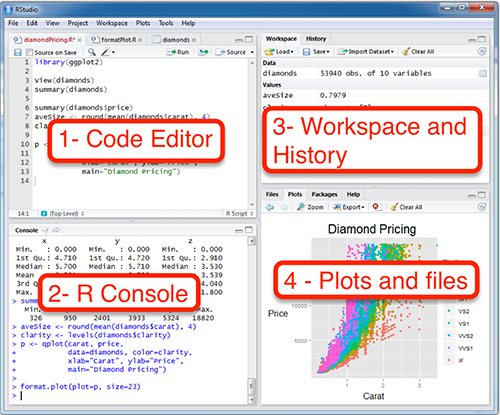
\includegraphics{images/01_01_rstudio.png}
\caption{}
\end{figure}

В первую очередь нас интересуют два окна: \textbf{1 - Code Editor} (окно
для написания скриптов) \footnote{При первом запуске RStudio вы не
  увидите это окно. Для того, чтобы оно появилось, нужно нажать
  \texttt{File\ -\ New\ File\ -\ R\ Script}.} и \textbf{2 - R Console}
(консоль). Здесь можно писать команды и запускать их. При этом работа в
консоли и работа со скриптом немного различается.

В \textbf{2 - R Console} вы пишите команду и запускаете ее нажиманием
\texttt{Enter}. Иногда после запуска команды появляется какой-то
результат. Если нажимать стрелку вверх на клавиатуре, то можно выводить
в консоль предыдущие команды. Это очень удобно для запуска предыдущих
команд с небольшими изменениями.

В \textbf{1 - Code Editor} для запуска команды вы должны выделить ее и
нажать \texttt{Ctrl} + \texttt{Enter} (\texttt{Cmd} + \texttt{Enter} на
macOS). Если не нажать эту комбинацию клавиш, то команда не запустится.
Можно выделить и запустить сразу несколько команд или даже все команды
скрипта. Все команды скрипта можно выделить с помощью сочетания клавиш
\texttt{Ctrl} + \texttt{A} на Windows и Linux, \texttt{Cmd} + \texttt{A}
на macOS \footnote{В RStudio есть много удобных сочетаний горячих
  клавиш. Чтобы посмотреть их все, нажмите
  \texttt{Help\ -\ Keyboard\ Shortcuts\ Help}.}. Как только вы запустите
команду (или несколько команд), соответствующие строчки кода появятся в
\textbf{2 - R Console}, как будто бы вы запускали их прямо там.

Обычно в консоли удобно что-то писать, чтобы быстро что-то посчитать.
Скрипты удобнее при работе с длинными командами и как способ сохранения
написанного кода для дальнейшей работы. Для сохранения скрипта нажмите
\texttt{File\ -\ Save\ As...}. R скрипты сохраняются с разрешением
\emph{.R}, но по своей сути это просто текстовые файлы, которые можно
открыть и модифицировать в любом текстовом редакторе а-ля ``Блокнот''.

\textbf{3 - Workspace and History} --- здесь можно увидеть переменные.
Это поле будет автоматически обновляться по мере того, как Вы будете
запускать строчки кода и создавать новые переменные. Еще там есть
вкладка с историей всех команд, которые были запущены.

\textbf{4 - Plots and files}. Здесь есть очень много всего. Во-первых,
небольшой файловый менеджер, во-вторых, там будут появляться графики,
когда вы будете их рисовать. Там же есть вкладка с вашими пакетами
(\texttt{Packages}) и \texttt{Help} по функциям. Но об этом потом.

\section{R как калькулятор}\label{calc}

R --- полноценный язык программирования, который позволяет решать
широкий спектр задач. Но в первую очередь R используется для анализа
данных и статистических вычислений. Тем не менее, многими R до сих пор
воспринимается как просто продвинутый калькулятор. Ну что ж,
калькулятор, так калькулятор.

Давайте начнем с самого простого и попробуем использовать R как
калькулятор с помощью арифметических операторов \texttt{+}, \texttt{-},
\texttt{*}, \texttt{/}, \texttt{\^{}} (степень), \texttt{()} и т.д.

Просто запускайте в консоли пока не надоест:

\begin{Shaded}
\begin{Highlighting}[]
\DecValTok{40}\OperatorTok{+}\DecValTok{2}
\end{Highlighting}
\end{Shaded}

\begin{verbatim}
## [1] 42
\end{verbatim}

\begin{Shaded}
\begin{Highlighting}[]
\DecValTok{3}\OperatorTok{-}\DecValTok{2}
\end{Highlighting}
\end{Shaded}

\begin{verbatim}
## [1] 1
\end{verbatim}

\begin{Shaded}
\begin{Highlighting}[]
\DecValTok{5}\OperatorTok{*}\DecValTok{6}
\end{Highlighting}
\end{Shaded}

\begin{verbatim}
## [1] 30
\end{verbatim}

\begin{Shaded}
\begin{Highlighting}[]
\DecValTok{99}\OperatorTok{/}\DecValTok{9} \CommentTok{#деление}
\end{Highlighting}
\end{Shaded}

\begin{verbatim}
## [1] 11
\end{verbatim}

\begin{Shaded}
\begin{Highlighting}[]
\DecValTok{2}\OperatorTok{^}\DecValTok{3} \CommentTok{#степень}
\end{Highlighting}
\end{Shaded}

\begin{verbatim}
## [1] 8
\end{verbatim}

\begin{Shaded}
\begin{Highlighting}[]
\DecValTok{13} \OperatorTok\StringTok{ }\DecValTok{3} \CommentTok{#целочисленное деление}
\end{Highlighting}
\end{Shaded}

\begin{verbatim}
## [1] 4
\end{verbatim}

\begin{Shaded}
\begin{Highlighting}[]
\DecValTok{13} \OperatorTok\StringTok{ }\DecValTok{3} \CommentTok{#остаток от деления}
\end{Highlighting}
\end{Shaded}

\begin{verbatim}
## [1] 1
\end{verbatim}

Попробуйте самостоятельно посчитать что-нибудь с разными числами.

\begin{figure}
\centering
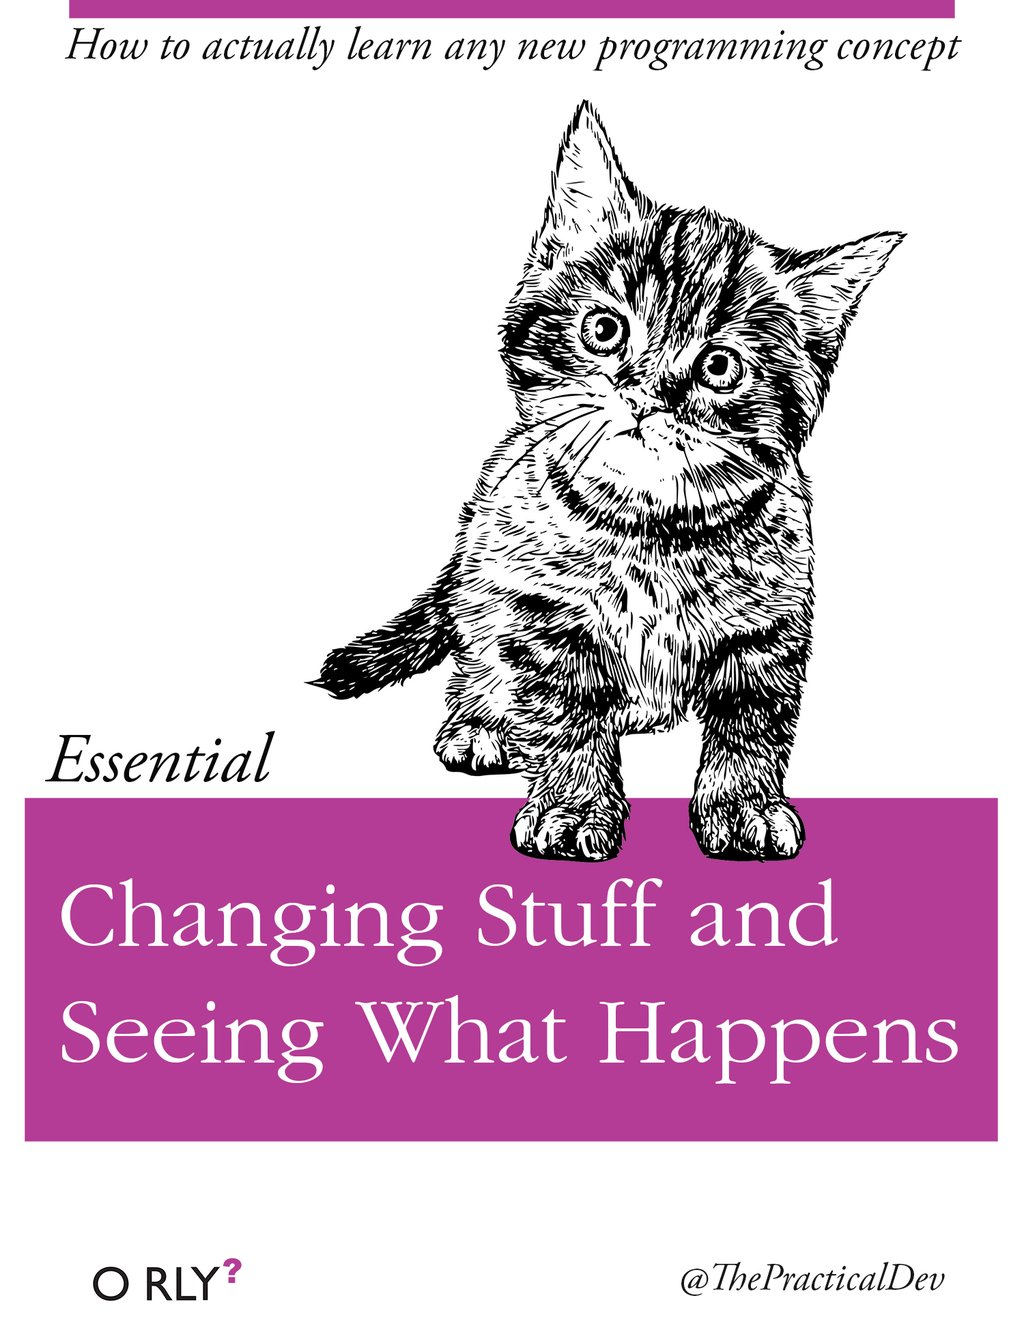
\includegraphics[width=4.16667in]{images/ThePracticalDev_2016-Apr-13.jpg}
\caption{}
\end{figure}

Ничего сложного, верно? Вводим выражение и получаем результат.

Вы могли заметить, что некоторые команды у меня заканчиваются знаком
решетки (\texttt{\#}). Все, что написано в строчке после \texttt{\#}
игнорируется R при выполнении команды. Написанные команды в скрипте
рекомендуется сопровождать комментариями, которые будут объяснять вам же
в будущем (или кому-то еще), что конкретно происходит в соответствующем
куске кода \footnote{Во время написания кода вам может казаться понятным
  то, что вы написали, но при возвращении к коду через некоторое время
  вы уже не будете этого помнить. Старайтесь писать комментарии как
  можно чаще!}. Кроме того, комментарии можно использовать в тех
случаях, когда вы хотите написать кусок кода по-другому, не стирая
полностью предыдущий код: достаточно ``закомментить'' нужные строчки -
поставить \texttt{\#} в начало каждой строки, которую вы хотите
переписать. Для этого есть специальное сочетание горячих клавиш:
\texttt{Ctrl} + \texttt{Shift} + \texttt{C} (\texttt{Cmd} +
\texttt{Shift} + \texttt{C} на macOS) --- во всех выделенных строчках
будет написан \texttt{\#} в начале.

Согласно данным навязчивых рекламных баннеров в интернете, только 14\%
россиян могут справиться с этим примером:

\begin{Shaded}
\begin{Highlighting}[]
\DecValTok{2} \OperatorTok{+}\StringTok{ }\DecValTok{2} \OperatorTok{*}\StringTok{ }\DecValTok{2}
\end{Highlighting}
\end{Shaded}

\begin{verbatim}
## [1] 6
\end{verbatim}

На самом деле, разные языки программирования ведут себя
\href{https://www.quora.com/Do-all-computer-languages-with-operator-precedence-use-the-same-operator-precedence}{по-разному}
в таких ситуациях, поэтому ответ 6 (сначала умножаем, потом складываем)
не так очевиден.

Порядок выполнения арифметических операций (т.е. приоритет операторов,
\emph{operator precedence}) в R как в математике, так что не забывайте
про скобочки.

\begin{Shaded}
\begin{Highlighting}[]
\NormalTok{(}\DecValTok{2}\OperatorTok{+}\DecValTok{2}\NormalTok{)}\OperatorTok{*}\DecValTok{2}
\end{Highlighting}
\end{Shaded}

\begin{verbatim}
## [1] 8
\end{verbatim}

Если Вы не уверены в том, какие операторы имеют приоритет, то
используйте скобочки, чтобы точно обозначить, в каком порядке нужно
производить операции. Или же смотрите на таблицу приоритета операторов с
помощью команды \texttt{?Syntax}.

\section{Функции}\label{func}

Давайте теперь извлечем корень из какого-нибудь числа. В принципе, тем,
кто помнит школьный курс математики, возведения в степень вполне
достаточно:

\begin{Shaded}
\begin{Highlighting}[]
\DecValTok{16}\OperatorTok{^}\FloatTok{0.5}
\end{Highlighting}
\end{Shaded}

\begin{verbatim}
## [1] 4
\end{verbatim}

Ну а если нет, то можете воспользоваться специальной \textbf{функцией}:
это обычно какие-то буквенные символы с круглыми скобками сразу после
названия функции. Мы подаем на вход (внутрь скобочек) какие-то данные,
внутри этих функций происходят какие-то вычисления, которые выдает в
ответ какие-то другие данные (или же функция записывает файл, рисует
график и т.д.).

Вот, например, функция для корня:

\begin{Shaded}
\begin{Highlighting}[]
\KeywordTok{sqrt}\NormalTok{(}\DecValTok{16}\NormalTok{)}
\end{Highlighting}
\end{Shaded}

\begin{verbatim}
## [1] 4
\end{verbatim}

\begin{quote}
R --- case-sensitive язык, т.е. регистр важен. SQRT(16) не будет
работать.
\end{quote}

А вот так выглядит функция логарифма:

\begin{Shaded}
\begin{Highlighting}[]
\KeywordTok{log}\NormalTok{(}\DecValTok{8}\NormalTok{)}
\end{Highlighting}
\end{Shaded}

\begin{verbatim}
## [1] 2.079442
\end{verbatim}

Так, вроде бы все нормально, но\ldots{} Если Вы еще что-то помните из
школьной математики, то должны понимать, что что-то здесь не так.

Здесь не хватает основания логарифма!

\begin{quote}
Логарифм --- показатель степени, в которую надо возвести число,
называемое основанием, чтобы получить данное число.
\end{quote}

То есть у логарифма 8 по основанию 2 будет значение 3:

\(\log_2 8 = 3\)

То есть если возвести 2 в степень 3 у нас будет 8:

\(2^3 = 8\)

Только наша функция считает все как-то не так.

Чтобы понять, что происходит, нам нужно залезть в хэлп этой функции:

\begin{Shaded}
\begin{Highlighting}[]
\NormalTok{?log}
\end{Highlighting}
\end{Shaded}

Справа внизу в RStudio появится вот такое окно:

\begin{figure}
\centering
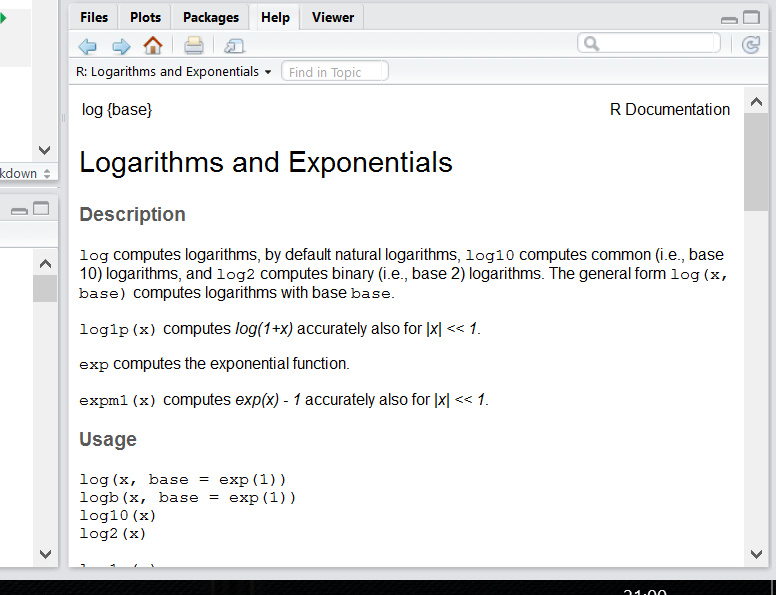
\includegraphics[width=4.16667in]{images/help.png}
\caption{}
\end{figure}

Действительно, у этой функции есть еще аргумент \emph{\texttt{base\ =}}.
По умолчанию он равен числу Эйлера (2.7182818\ldots{}), т.е. функция
считает натуральный логарифм. В большинстве функций R есть какой-то
основной инпут --- данные в том или ином формате, а есть и
дополнительные параметры, которые можно прописывать вручную, если
параметры по умолчанию вас не устраивают.

\begin{Shaded}
\begin{Highlighting}[]
\KeywordTok{log}\NormalTok{(}\DataTypeTok{x =} \DecValTok{8}\NormalTok{, }\DataTypeTok{base =} \DecValTok{2}\NormalTok{)}
\end{Highlighting}
\end{Shaded}

\begin{verbatim}
## [1] 3
\end{verbatim}

\ldots{}или просто (если Вы уверены в порядке переменных):

\begin{Shaded}
\begin{Highlighting}[]
\KeywordTok{log}\NormalTok{(}\DecValTok{8}\NormalTok{,}\DecValTok{2}\NormalTok{)}
\end{Highlighting}
\end{Shaded}

\begin{verbatim}
## [1] 3
\end{verbatim}

Более того, Вы можете использовать результат выполнения одних функций в
качестве аргумента для других:

\begin{Shaded}
\begin{Highlighting}[]
\KeywordTok{log}\NormalTok{(}\DecValTok{8}\NormalTok{, }\KeywordTok{sqrt}\NormalTok{(}\DecValTok{4}\NormalTok{))}
\end{Highlighting}
\end{Shaded}

\begin{verbatim}
## [1] 3
\end{verbatim}

Если эксплицитно писать имена аргументов, то их порядок в функции не
важен:

\begin{Shaded}
\begin{Highlighting}[]
\KeywordTok{log}\NormalTok{(}\DataTypeTok{base =} \DecValTok{2}\NormalTok{, }\DataTypeTok{x =} \DecValTok{8}\NormalTok{)}
\end{Highlighting}
\end{Shaded}

\begin{verbatim}
## [1] 3
\end{verbatim}

А еще можно недописывать имена аргументов, если они не совпадают с
другими:

\begin{Shaded}
\begin{Highlighting}[]
\KeywordTok{log}\NormalTok{(}\DataTypeTok{b =} \DecValTok{2}\NormalTok{, }\DataTypeTok{x =} \DecValTok{8}\NormalTok{)}
\end{Highlighting}
\end{Shaded}

\begin{verbatim}
## [1] 3
\end{verbatim}

Мы еще много раз будем возвращаться к функциям. Вообще, функции --- это
одна из важнейших штук в R (примерно так же как и в Python). Мы будем
создавать свои функции, использовать функции как инпут для функций и
многое-многое другое. В R очень крутые возможности работы с функциями.
Поэтому подружитесь с функциями, они клевые.

\begin{quote}
Арифметические знаки, которые мы использовали: +,-,/,\^{} и т.д.
называются \textbf{операторами} и на самом деле тоже являются функциями:
\end{quote}

\begin{Shaded}
\begin{Highlighting}[]
\StringTok{'+'}\NormalTok{(}\DecValTok{3}\NormalTok{,}\DecValTok{4}\NormalTok{)}
\end{Highlighting}
\end{Shaded}

\begin{verbatim}
## [1] 7
\end{verbatim}

\section{В любой непонятной ситуации --- гуглите}\label{google}

Если вдруг вы не знаете, что искать в хэлпе, или хэлпа попросту
недостаточно, то\ldots{} гуглите!

\begin{figure}
\centering
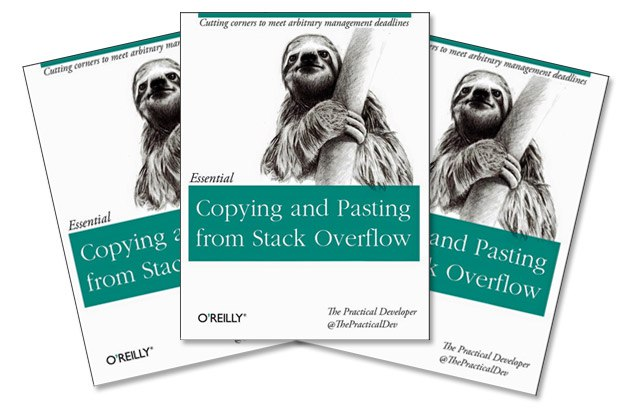
\includegraphics[width=4.16667in]{images/2AmXWgVoULk.jpg}
\caption{}
\end{figure}

Нет ничего постыдного в том, чтобы гуглить решения проблем. Это
абсолютно нормально. Используйте силу интернета во благо и да помогут
вам \emph{Stackoverflow}\footnote{Stackoverflow --- это сайт с вопросами
  и ответами. Эдакий аналог \emph{Quora}, \emph{The Question}, ну или
  \emph{Ответы Mail.ru} в мире программирования.} и бесчисленные
R-туториалы!

Computer Programming To Be Officially Renamed ``Googling Stack
Overflow''Source: http://t.co/xu7acfXvFF pic.twitter.com/iJ9k7aAVhd

--- Stack Exchange (\citet{StackExchange}) July 20, 2015

\begin{figure}
\centering

\includegraphics[width=4.16667in]{images/doctors-googling-stuff-online-does-not-make-you-a-doctor-programmers-confused.jpg}
\caption{}
\end{figure}

Главное, помните: загуглить работающий ответ всегда недостаточно. Надо
понять, как и почему решение работает. Иначе что-то обязательно пойдет
не так.

Кроме того, правильно загуглить проблему --- не так уж и просто.

Does anyone ever get good at R or do they just get good at googling how
to do things in R

--- 🔬🖤Lauren M. Seyler, Ph.D.❤️⚒ (\citet{mousquemere}) May 6, 2019

Короче говоря: гуглить --- хорошо, бездумно копировать чужие решения ---
плохо.

\section{Переменные}\label{variables}

Важная штука в программировании на практически любом языке ---
возможность сохранять значения в \textbf{переменных}. В R это обычно
делается с помощью вот этих символов: \texttt{\textless{}-} (но можно
использовать и обычное \texttt{=}, хотя это не очень принято). Для этого
есть удобное сочетание клавиш: нажмите одновременно \texttt{Alt} +
\texttt{-} (или \texttt{option} + \texttt{-} на macOS).

\begin{quote}
Заметьте, при присвоении результат вычисления не выводится в консоль!
Если опустить детали, то обычно результат выполнения комманды либо
выводится в консоль, либо записывается в переменную.
\end{quote}

\begin{Shaded}
\begin{Highlighting}[]
\NormalTok{a <-}\StringTok{ }\DecValTok{2}
\NormalTok{a}
\end{Highlighting}
\end{Shaded}

\begin{verbatim}
## [1] 2
\end{verbatim}

Справа от \texttt{\textless{}-} находится значение, которое вы хотите
сохранить, или же какое-то выражение, результат которого вы хотите
сохранить в эту переменную\footnote{Есть еще оператор
  \texttt{-\textgreater{}}, который позволяет присваивать значения слева
  направо, но так делать не рекомендуется, хотя это бывает довольно
  удобным.}:

Слева от \texttt{\textless{}-} находится название будущей переменной.
Название переменных может быть самым разным. Есть несколько ограничений
для синтаксически валидных имен переменных: они должны включать в себя
буквы, цифры, \texttt{.} или \texttt{\_}, начинаться на букву (или
точку, за которой не будет следовать цифра), не должны совпадать с
\href{https://stat.ethz.ch/R-manual/R-devel/library/base/html/Reserved.html}{коротким
списком зарезервированных слов}. Короче говоря, название не должно
включать в себя пробелы и большинство других знаков.

Нельзя: - \texttt{new\ variable} - \texttt{\_new\_variable} -
\texttt{.1var} - \texttt{v-r}

Можно: - \texttt{new\_variable} - \texttt{.new.variable} -
\texttt{var\_2}

Обязательно делайте названия переменных осмысленными! Старайтесь делать
при этом их понятными и короткими, это сохранит вам очень много времени,
когда вы (или кто-то еще) будете пытаться разобраться в написанном ранее
коде. Если название все-таки получается длинным и состоящим из
нескольких слов, то лучше всего использовать нижнее подчеркивание в
качестве разделителя: \texttt{some\_variable}\footnote{Еще иногда
  используются большие буквы \texttt{SomeVariable}, но это плохо
  читается, а иногда --- точка, но это тоже не рекомендуется.}.

После присвоения переменная появляется во вкладке \textbf{Environment} в
RStudio:

\begin{figure}
\centering
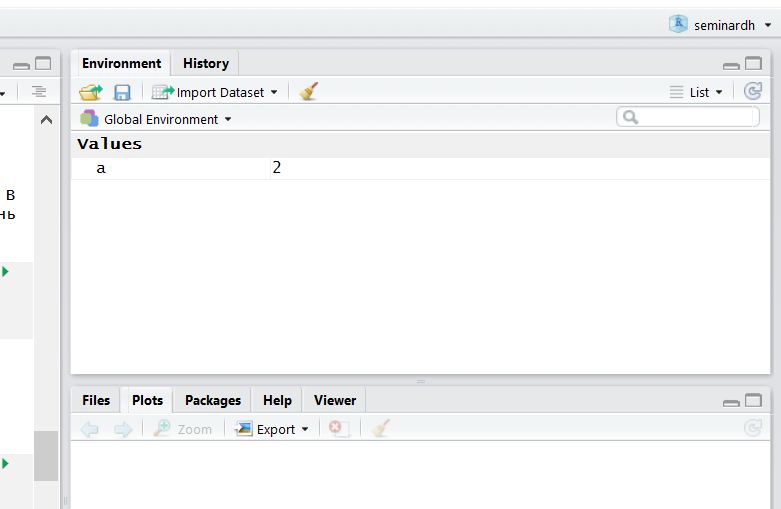
\includegraphics[width=4.16667in]{images/env.png}
\caption{}
\end{figure}

Можно использовать переменные в функциях и просто вычислениях:

\begin{Shaded}
\begin{Highlighting}[]
\NormalTok{b <-}\StringTok{ }\NormalTok{a }\OperatorTok{^}\StringTok{ }\NormalTok{a }\OperatorTok{+}\StringTok{ }\NormalTok{a }\OperatorTok{*}\StringTok{ }\NormalTok{a}
\NormalTok{b}
\end{Highlighting}
\end{Shaded}

\begin{verbatim}
## [1] 8
\end{verbatim}

\begin{Shaded}
\begin{Highlighting}[]
\KeywordTok{log}\NormalTok{(b, a)}
\end{Highlighting}
\end{Shaded}

\begin{verbatim}
## [1] 3
\end{verbatim}

\section{Логические операторы}\label{logic}

Вы можете сравнивать разные переменные:

\begin{Shaded}
\begin{Highlighting}[]
\NormalTok{a }\OperatorTok{==}\StringTok{ }\NormalTok{b}
\end{Highlighting}
\end{Shaded}

\begin{verbatim}
## [1] FALSE
\end{verbatim}

Заметьте, что сравнивая две переменные мы используем два знака равно
\texttt{==}, а не один \texttt{=}. Иначе это будет означать присвоение.

\begin{Shaded}
\begin{Highlighting}[]
\NormalTok{a =}\StringTok{ }\NormalTok{b}
\NormalTok{a}
\end{Highlighting}
\end{Shaded}

\begin{verbatim}
## [1] 8
\end{verbatim}

Теперь Вы сможете понять комикс про восстание роботов на следующей
странице (пусть он и совсем про другой язык программирования)

\begin{figure}
\centering
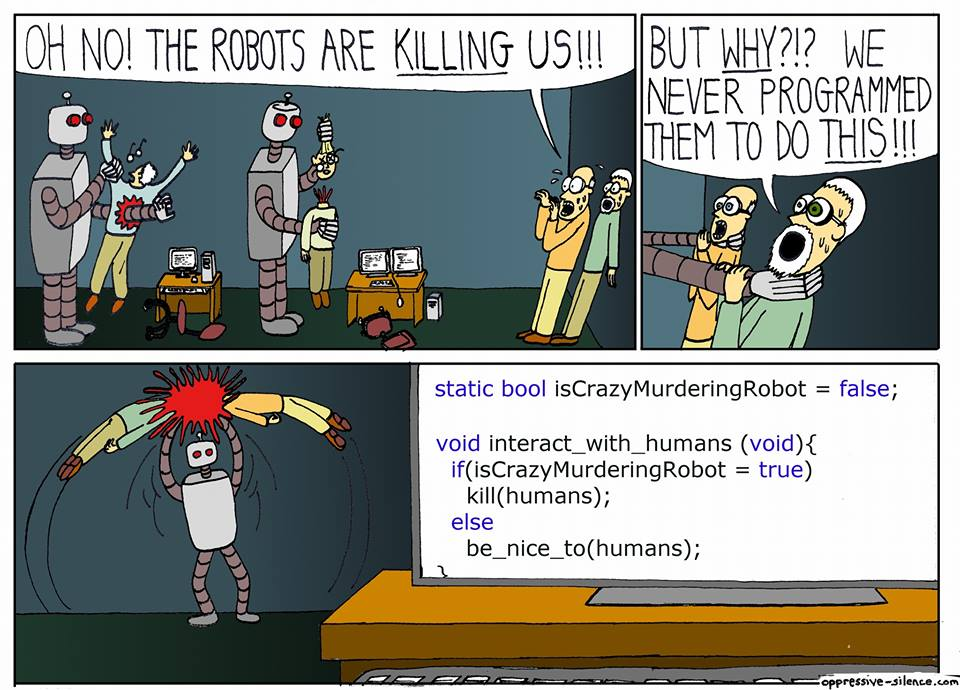
\includegraphics[width=4.16667in]{images/WaCM5x3mvQM.jpg}
\caption{}
\end{figure}

Этот комикс объясняет, как важно не путать присваивание и сравнение
\emph{(хотя я иногда путаю до сих пор =( )}.

Иногда нам нужно проверить на \emph{не}равенство:

\begin{Shaded}
\begin{Highlighting}[]
\NormalTok{a <-}\StringTok{ }\DecValTok{2}
\NormalTok{b <-}\StringTok{ }\DecValTok{3}

\NormalTok{a }\OperatorTok{==}\StringTok{ }\NormalTok{b}
\end{Highlighting}
\end{Shaded}

\begin{verbatim}
## [1] FALSE
\end{verbatim}

\begin{Shaded}
\begin{Highlighting}[]
\NormalTok{a }\OperatorTok{!=}\StringTok{ }\NormalTok{b}
\end{Highlighting}
\end{Shaded}

\begin{verbatim}
## [1] TRUE
\end{verbatim}

Восклицательный язык в программировании вообще и в R в частности
стандартно означает отрицание.

Еще мы можем сравнивать на больше/меньше:

\begin{Shaded}
\begin{Highlighting}[]
\NormalTok{a }\OperatorTok{>}\StringTok{ }\NormalTok{b}
\end{Highlighting}
\end{Shaded}

\begin{verbatim}
## [1] FALSE
\end{verbatim}

\begin{Shaded}
\begin{Highlighting}[]
\NormalTok{a }\OperatorTok{<}\StringTok{ }\NormalTok{b}
\end{Highlighting}
\end{Shaded}

\begin{verbatim}
## [1] TRUE
\end{verbatim}

\begin{Shaded}
\begin{Highlighting}[]
\NormalTok{a }\OperatorTok{>=}\StringTok{ }\NormalTok{b}
\end{Highlighting}
\end{Shaded}

\begin{verbatim}
## [1] FALSE
\end{verbatim}

\begin{Shaded}
\begin{Highlighting}[]
\NormalTok{a }\OperatorTok{<=}\StringTok{ }\NormalTok{b}
\end{Highlighting}
\end{Shaded}

\begin{verbatim}
## [1] TRUE
\end{verbatim}

Этим мы будем пользоваться в дальнейшем регулярно! Именно на таких
простых логических операциях построено большинство операций с данными.

\section{Типы данных}\label{data_types}

До этого момента мы работали только с числами (numeric):

\begin{Shaded}
\begin{Highlighting}[]
\KeywordTok{class}\NormalTok{(a)}
\end{Highlighting}
\end{Shaded}

\begin{verbatim}
## [1] "numeric"
\end{verbatim}

На самом деле, в R три типа numeric: integer (целые), double (дробные),
complex (комплексные числа)\footnote{Комплексные числа в R пишутся так:
  \texttt{complexnumber\ \textless{}-\ 2+2i}. \texttt{i} здесь - это та
  самая мнимая единица, которая является квадратным корнем из -1.}. R
сам будет конвертировать числа в нужный тип numeric при необходимости,
поэтому этим можно не заморачиваться.

Если же все-таки нужно задать конкретный тип числа эксплицитно, то можно
воспользоваться функциями \texttt{as.integer()}, \texttt{as.double()} и
\texttt{as.complex()}. Кроме того, при создании числа можно поставить в
конце \texttt{L}, чтобы обозначить число как integer:

\begin{Shaded}
\begin{Highlighting}[]
\KeywordTok{is.integer}\NormalTok{(}\DecValTok{5}\NormalTok{)}
\end{Highlighting}
\end{Shaded}

\begin{verbatim}
## [1] FALSE
\end{verbatim}

\begin{Shaded}
\begin{Highlighting}[]
\KeywordTok{is.integer}\NormalTok{(5L)}
\end{Highlighting}
\end{Shaded}

\begin{verbatim}
## [1] TRUE
\end{verbatim}

Про double есть еще один маленький секрет. Дело в том, что дробные числа
хранятся в R как
\href{https://ru.wikipedia.org/wiki/Число_двойной_точности}{числа с
плавающей запятой двойной точности}. Дробные числа в компьютере могут
быть записаны только с определенной степенью точности, поэтому иногда
встречаются вот такие вот ситуации:

\begin{Shaded}
\begin{Highlighting}[]
\KeywordTok{sqrt}\NormalTok{(}\DecValTok{2}\NormalTok{)}\OperatorTok{^}\DecValTok{2} \OperatorTok{==}\StringTok{ }\DecValTok{2}
\end{Highlighting}
\end{Shaded}

\begin{verbatim}
## [1] FALSE
\end{verbatim}

Это довольно стандартная ситуация, характерная не только для R. Чтобы ее
избежать, можно воспользоваться функцией \texttt{all.equal()}:

\begin{Shaded}
\begin{Highlighting}[]
\KeywordTok{all.equal}\NormalTok{(}\KeywordTok{sqrt}\NormalTok{(}\DecValTok{2}\NormalTok{)}\OperatorTok{^}\DecValTok{2}\NormalTok{, }\DecValTok{2}\NormalTok{)}
\end{Highlighting}
\end{Shaded}

\begin{verbatim}
## [1] TRUE
\end{verbatim}

Теперь нам нужно ознакомиться с двумя другими важными типами данных в R:

\begin{enumerate}
\def\labelenumi{\arabic{enumi}.}
\tightlist
\item
  \textbf{Строковые} данные (\textbf{character}): набор букв, цифр и
  символов, которые должны выделяться кавычками.
\end{enumerate}

\begin{Shaded}
\begin{Highlighting}[]
\NormalTok{s <-}\StringTok{ "Всем привет!"}
\NormalTok{s}
\end{Highlighting}
\end{Shaded}

\begin{verbatim}
## [1] "Всем привет!"
\end{verbatim}

\begin{Shaded}
\begin{Highlighting}[]
\KeywordTok{class}\NormalTok{(s)}
\end{Highlighting}
\end{Shaded}

\begin{verbatim}
## [1] "character"
\end{verbatim}

Можно использовать как \texttt{"}, так и \texttt{\textquotesingle{}}
(что удобно, когда строчка внутри уже содержит какие-то кавычки).

\begin{Shaded}
\begin{Highlighting}[]
\StringTok{"Ph'nglui mglw'nafh Cthulhu R'lyeh wgah'nagl fhtagn"}
\end{Highlighting}
\end{Shaded}

\begin{verbatim}
## [1] "Ph'nglui mglw'nafh Cthulhu R'lyeh wgah'nagl fhtagn"
\end{verbatim}

\begin{enumerate}
\def\labelenumi{\arabic{enumi}.}
\setcounter{enumi}{1}
\tightlist
\item
  \textbf{logical}: просто \texttt{TRUE} или \texttt{FALSE}.
\end{enumerate}

\begin{Shaded}
\begin{Highlighting}[]
\NormalTok{t1 <-}\StringTok{ }\OtherTok{TRUE}
\NormalTok{f1 <-}\StringTok{ }\OtherTok{FALSE}

\NormalTok{t1}
\end{Highlighting}
\end{Shaded}

\begin{verbatim}
## [1] TRUE
\end{verbatim}

\begin{Shaded}
\begin{Highlighting}[]
\NormalTok{f1}
\end{Highlighting}
\end{Shaded}

\begin{verbatim}
## [1] FALSE
\end{verbatim}

Вообще, можно еще писать \texttt{T} и \texttt{F} (но не \texttt{True} и
\texttt{False}!)

\begin{Shaded}
\begin{Highlighting}[]
\NormalTok{t2 <-}\StringTok{ }\NormalTok{T}
\NormalTok{f2 <-}\StringTok{ }\NormalTok{F}
\end{Highlighting}
\end{Shaded}

Это дурная практика, так как R защищает от перезаписи переменные
\texttt{TRUE} и \texttt{FALSE}, но не защищает от этого \texttt{T} и
\texttt{F}.

\begin{Shaded}
\begin{Highlighting}[]
\OtherTok{TRUE}\NormalTok{ <-}\StringTok{ }\OtherTok{FALSE}
\end{Highlighting}
\end{Shaded}

\begin{verbatim}
## Error in TRUE <- FALSE: неправильная (do_set) левая сторона в присвоении
\end{verbatim}

\begin{Shaded}
\begin{Highlighting}[]
\OtherTok{TRUE}
\end{Highlighting}
\end{Shaded}

\begin{verbatim}
## [1] TRUE
\end{verbatim}

\begin{Shaded}
\begin{Highlighting}[]
\NormalTok{T <-}\StringTok{ }\OtherTok{FALSE}
\NormalTok{T}
\end{Highlighting}
\end{Shaded}

\begin{verbatim}
## [1] FALSE
\end{verbatim}

Функция \texttt{rm()} позволяет удалить ненужную переменную:

Мы уже встречались с логическими значениями при сравнении двух числовых
переменных. Теперь вы можете догадаться, что результаты сравнения,
например, числовых или строковых переменных, можно тоже сохранять в
переменные!

\begin{Shaded}
\begin{Highlighting}[]
\NormalTok{comparison <-}\StringTok{ }\NormalTok{a }\OperatorTok{==}\StringTok{ }\NormalTok{b}
\NormalTok{comparison}
\end{Highlighting}
\end{Shaded}

\begin{verbatim}
## [1] FALSE
\end{verbatim}

Это нам очень понадобится, когда мы будем работать с реальными данными:
нам нужно будет постоянно вытаскивать какие-то данные из датасета, что
как раз и построено на игре со сравнением переменных.\\
Чтобы этим хорошо уметь пользоваться, нам нужно еще освоить как работать
с логическими операторами. Про один мы немного уже говорили --- это
логическое НЕ (\texttt{!}). \texttt{!} превращает \texttt{TRUE} в
\texttt{FALSE}, а \texttt{FALSE} в \texttt{TRUE}:

\begin{Shaded}
\begin{Highlighting}[]
\NormalTok{t1}
\end{Highlighting}
\end{Shaded}

\begin{verbatim}
## [1] TRUE
\end{verbatim}

\begin{Shaded}
\begin{Highlighting}[]
\OperatorTok{!}\NormalTok{t1}
\end{Highlighting}
\end{Shaded}

\begin{verbatim}
## [1] FALSE
\end{verbatim}

\begin{Shaded}
\begin{Highlighting}[]
\OperatorTok{!!}\NormalTok{t1 }\CommentTok{#Двойное отрицание!}
\end{Highlighting}
\end{Shaded}

\begin{verbatim}
## [1] TRUE
\end{verbatim}

Еще есть логическое И (выдаст \texttt{TRUE} только в том случае если обе
переменные \texttt{TRUE}):

\begin{Shaded}
\begin{Highlighting}[]
\NormalTok{t1 }\OperatorTok{&}\StringTok{ }\NormalTok{t2}
\end{Highlighting}
\end{Shaded}

\begin{verbatim}
## [1] TRUE
\end{verbatim}

\begin{Shaded}
\begin{Highlighting}[]
\NormalTok{t1 }\OperatorTok{&}\StringTok{ }\NormalTok{f1}
\end{Highlighting}
\end{Shaded}

\begin{verbatim}
## [1] FALSE
\end{verbatim}

А еще логическое ИЛИ (выдаст \texttt{TRUE} в случае если хотя бы одна из
переменных \texttt{TRUE}):

\begin{Shaded}
\begin{Highlighting}[]
\NormalTok{t1 }\OperatorTok{|}\StringTok{ }\NormalTok{f1}
\end{Highlighting}
\end{Shaded}

\begin{verbatim}
## [1] TRUE
\end{verbatim}

\begin{Shaded}
\begin{Highlighting}[]
\NormalTok{f1 }\OperatorTok{|}\StringTok{ }\NormalTok{f2}
\end{Highlighting}
\end{Shaded}

\begin{verbatim}
## [1] FALSE
\end{verbatim}

Если кому-то вдруг понадобится другое ИЛИ (строгое ЛИБО) --- есть
функция \texttt{xor()}, принимающая два аргумента и возвращая
\texttt{TRUE} только в том случае, если ровно один из двух аргументов
равен \texttt{TRUE}.

Итак, мы только что разобрались с самой занудной (хотя и важной) частью
- с основными типа данных в R и как с ними работать\footnote{Кроме
  описанных пяти типов данных (integer, double, complex, character и
  logical) есть еще и шестой --- это raw, сырая последовательность
  байтов, но нам она не понадобится.}. Пора переходить к чему-то более
интересному и специфическому для R. Вперед к ВЕКТОРАМ!

\chapter{Вектор}\label{vector}

\section{Понятие atomic вектора в R}\label{atomic}

Если у вас не было линейной алгебры (или у вас с ней было все плохо), то
просто запомните, что \textbf{вектор} (\textbf{atomic vector} или просто
\textbf{atomic}) --- это набор (столбик) чисел в определенном порядке.

Если вы привыкли из школьного курса физики считать вектора стрелочками,
то не спешите возмущаться и паниковать. Представьте стрелочки как точки
из нуля координат \{0,0\} до какой-то точки на координатной плоскости,
например, \{2,3\}:

\begin{figure}
\centering
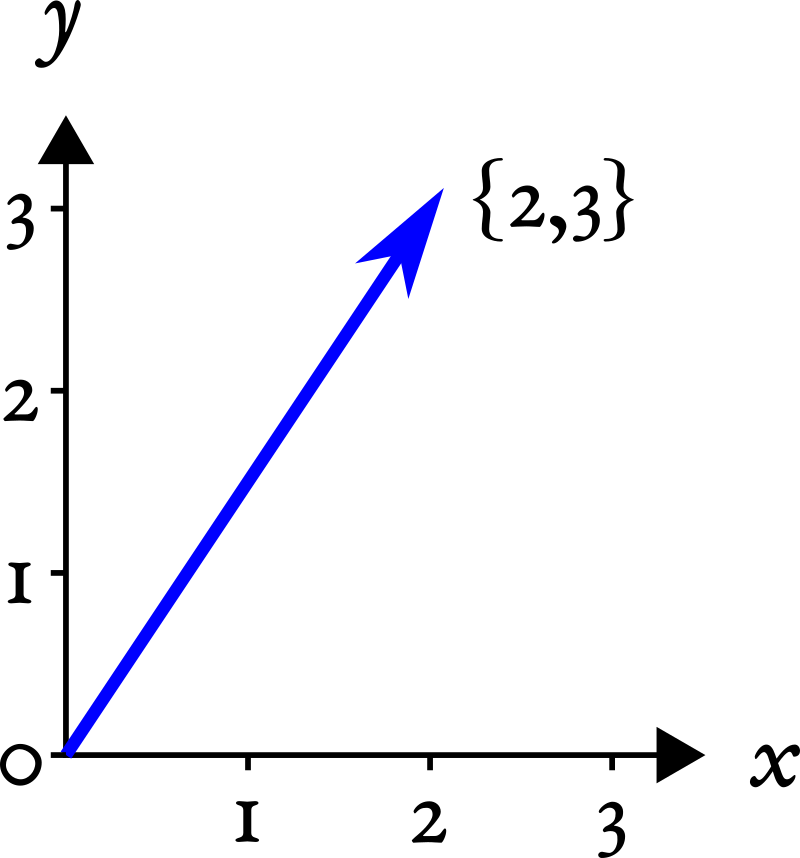
\includegraphics[width=4.16667in]{images/coord_vector.png}
\caption{}
\end{figure}

Вот последние два числа и будем считать вектором. Попытайтесь теперь
мысленно стереть координатную плоскость и выбросить стрелочки из головы,
оставив только последовательность чисел \{2,3\}:

\begin{figure}
\centering
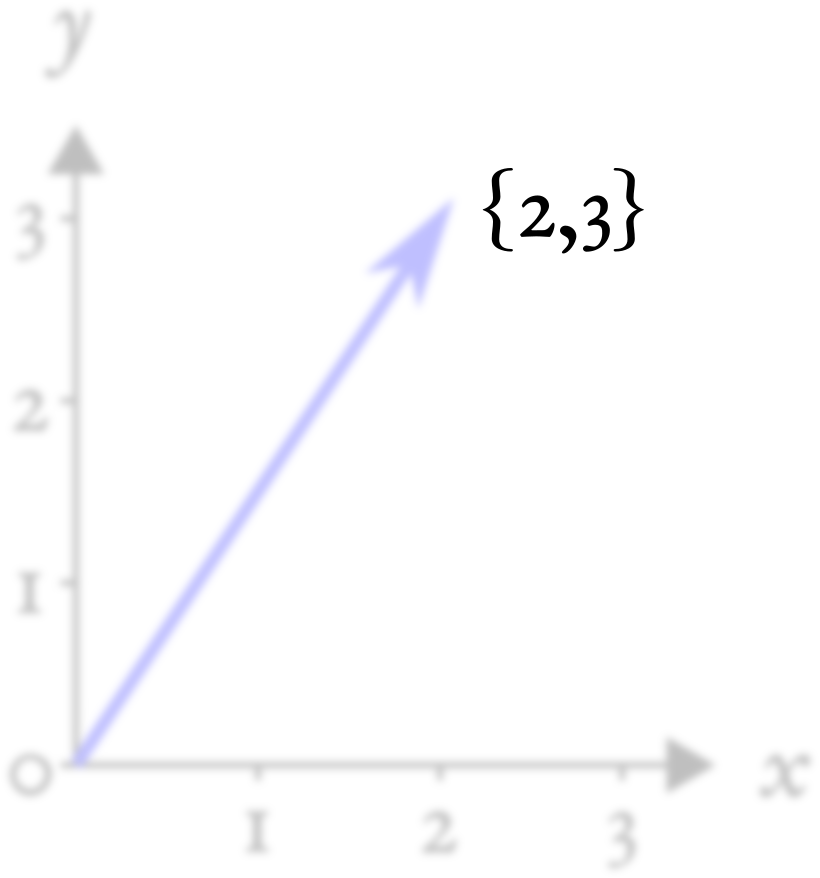
\includegraphics[width=4.16667in]{images/coord_vector_blur.png}
\caption{}
\end{figure}

На самом деле, мы уже работали с векторами в R, но, возможно, вы об этом
даже не догадывались. Дело в том, что в R нет как таковых скалярных
(т.е. одиночных) значений, \textbf{есть вектора длиной 1}. Такие дела!

Чтобы создать вектор из нескольких значений, нужно воспользоваться
функцией \emph{\texttt{c()}}:

\begin{Shaded}
\begin{Highlighting}[]
\KeywordTok{c}\NormalTok{(}\DecValTok{4}\NormalTok{, }\DecValTok{8}\NormalTok{, }\DecValTok{15}\NormalTok{, }\DecValTok{16}\NormalTok{, }\DecValTok{23}\NormalTok{, }\DecValTok{42}\NormalTok{)}
\end{Highlighting}
\end{Shaded}

\begin{verbatim}
## [1]  4  8 15 16 23 42
\end{verbatim}

\begin{Shaded}
\begin{Highlighting}[]
\KeywordTok{c}\NormalTok{(}\StringTok{"Хэй"}\NormalTok{, }\StringTok{"Хэй"}\NormalTok{, }\StringTok{"Ха"}\NormalTok{)}
\end{Highlighting}
\end{Shaded}

\begin{verbatim}
## [1] "Хэй" "Хэй" "Ха"
\end{verbatim}

\begin{Shaded}
\begin{Highlighting}[]
\KeywordTok{c}\NormalTok{(}\OtherTok{TRUE}\NormalTok{, }\OtherTok{FALSE}\NormalTok{)}
\end{Highlighting}
\end{Shaded}

\begin{verbatim}
## [1]  TRUE FALSE
\end{verbatim}

\begin{quote}
Одна из самых мерзких и раздражающих причин ошибок в коде --- это
использование \texttt{с} из кириллицы вместо \texttt{c} из латиницы.
Видите разницу? И я не вижу. А R видит. И об этом сообщает:
\end{quote}

\begin{Shaded}
\begin{Highlighting}[]
\NormalTok{с(}\DecValTok{3}\NormalTok{, }\DecValTok{4}\NormalTok{, }\DecValTok{5}\NormalTok{)}
\end{Highlighting}
\end{Shaded}

\begin{verbatim}
## Error in с(3, 4, 5): не могу найти функцию "с"
\end{verbatim}

Для создания числовых векторов есть удобный \textbf{оператор} \texttt{:}

\begin{Shaded}
\begin{Highlighting}[]
\DecValTok{1}\OperatorTok{:}\DecValTok{10}
\end{Highlighting}
\end{Shaded}

\begin{verbatim}
##  [1]  1  2  3  4  5  6  7  8  9 10
\end{verbatim}

\begin{Shaded}
\begin{Highlighting}[]
\DecValTok{5}\OperatorTok{:-}\DecValTok{3}
\end{Highlighting}
\end{Shaded}

\begin{verbatim}
## [1]  5  4  3  2  1  0 -1 -2 -3
\end{verbatim}

Этот оператор создает вектор от первого числа до второго с шагом 1. Вы
не представляете, как часто эта штука нам пригодится\ldots{} Если же
нужно сделать вектор с другим шагом, то есть функция \texttt{seq()}:

\begin{Shaded}
\begin{Highlighting}[]
\KeywordTok{seq}\NormalTok{(}\DecValTok{10}\NormalTok{,}\DecValTok{100}\NormalTok{, }\DataTypeTok{by =} \DecValTok{10}\NormalTok{)}
\end{Highlighting}
\end{Shaded}

\begin{verbatim}
##  [1]  10  20  30  40  50  60  70  80  90 100
\end{verbatim}

Кроме того, можно задавать не шаг, а длину вектора. Тогда функция
\texttt{seq()} сама посчитает шаг:

\begin{Shaded}
\begin{Highlighting}[]
\KeywordTok{seq}\NormalTok{(}\DecValTok{1}\NormalTok{,}\DecValTok{13}\NormalTok{, }\DataTypeTok{length.out =} \DecValTok{4}\NormalTok{)}
\end{Highlighting}
\end{Shaded}

\begin{verbatim}
## [1]  1  5  9 13
\end{verbatim}

Другая функция --- \texttt{rep()} --- позволяет создавать вектора с
повторяющимися значениями. Первый аргумент --- значение, которое нужно
повторять, а второй аргумент --- сколько раз повторять.

\begin{Shaded}
\begin{Highlighting}[]
\KeywordTok{rep}\NormalTok{(}\DecValTok{1}\NormalTok{, }\DecValTok{5}\NormalTok{)}
\end{Highlighting}
\end{Shaded}

\begin{verbatim}
## [1] 1 1 1 1 1
\end{verbatim}

И первый, и второй аргумент могут быть векторами!

\begin{Shaded}
\begin{Highlighting}[]
\KeywordTok{rep}\NormalTok{(}\DecValTok{1}\OperatorTok{:}\DecValTok{3}\NormalTok{, }\DecValTok{3}\NormalTok{)}
\end{Highlighting}
\end{Shaded}

\begin{verbatim}
## [1] 1 2 3 1 2 3 1 2 3
\end{verbatim}

\begin{Shaded}
\begin{Highlighting}[]
\KeywordTok{rep}\NormalTok{(}\DecValTok{1}\OperatorTok{:}\DecValTok{3}\NormalTok{, }\DecValTok{1}\OperatorTok{:}\DecValTok{3}\NormalTok{)}
\end{Highlighting}
\end{Shaded}

\begin{verbatim}
## [1] 1 2 2 3 3 3
\end{verbatim}

Еще можно объединять вектора (что мы, по сути, и делали, просто с
векторами длиной 1):

\begin{Shaded}
\begin{Highlighting}[]
\NormalTok{v1 <-}\StringTok{ }\KeywordTok{c}\NormalTok{(}\StringTok{"Hey"}\NormalTok{, }\StringTok{"Ho"}\NormalTok{)}
\NormalTok{v2 <-}\StringTok{ }\KeywordTok{c}\NormalTok{(}\StringTok{"Let's"}\NormalTok{, }\StringTok{"Go!"}\NormalTok{)}
\KeywordTok{c}\NormalTok{(v1, v2)}
\end{Highlighting}
\end{Shaded}

\begin{verbatim}
## [1] "Hey"   "Ho"    "Let's" "Go!"
\end{verbatim}

Очень многие функции в R работают именно с векторами. Например, функции
\texttt{sum()} (считает сумму значений вектора) и \texttt{mean()}
(считает среднее арифметическое всех значений в векторе):

\begin{Shaded}
\begin{Highlighting}[]
\KeywordTok{sum}\NormalTok{(}\DecValTok{1}\OperatorTok{:}\DecValTok{10}\NormalTok{)}
\end{Highlighting}
\end{Shaded}

\begin{verbatim}
## [1] 55
\end{verbatim}

\begin{Shaded}
\begin{Highlighting}[]
\KeywordTok{mean}\NormalTok{(}\DecValTok{1}\OperatorTok{:}\DecValTok{10}\NormalTok{)}
\end{Highlighting}
\end{Shaded}

\begin{verbatim}
## [1] 5.5
\end{verbatim}

\section{Приведение типов}\label{coercion}

Что будет, если вы объедините два вектора с значениями разных типов?
Ошибка?

Мы уже обсуждали, что в обычных векторах (\emph{atomic} векторах) может
быть только один тип данных. В некоторых языках программирования при
операции с данными разных типов мы бы получили ошибку. А вот в R при
несовпадении типов произойдет попытка привести типы к ``общему
знаменателю'', то есть конвертировать данные в более ``широкий'' тип (а
иногда --- более ``узкий'' тип, если того требует функция).

Например:

\begin{Shaded}
\begin{Highlighting}[]
\KeywordTok{c}\NormalTok{(}\OtherTok{FALSE}\NormalTok{, }\DecValTok{2}\NormalTok{)}
\end{Highlighting}
\end{Shaded}

\begin{verbatim}
## [1] 0 2
\end{verbatim}

\texttt{FALSE} превратился в \texttt{0} (а \texttt{TRUE} превратился бы
в \texttt{1}), чтобы оба значения можно было объединить в вектор. То же
самое произошло бы в случае операций с векторами:

\begin{Shaded}
\begin{Highlighting}[]
\DecValTok{2} \OperatorTok{+}\StringTok{ }\OtherTok{TRUE}
\end{Highlighting}
\end{Shaded}

\begin{verbatim}
## [1] 3
\end{verbatim}

Это называется \textbf{неявным приведением типов (implicit coercion)}.

Вот более сложный пример:

\begin{Shaded}
\begin{Highlighting}[]
\KeywordTok{c}\NormalTok{(}\OtherTok{TRUE}\NormalTok{, }\DecValTok{3}\NormalTok{, }\StringTok{"Привет"}\NormalTok{)}
\end{Highlighting}
\end{Shaded}

\begin{verbatim}
## [1] "TRUE"   "3"      "Привет"
\end{verbatim}

Здесь все значения были приведены сразу к строковому типу данных.

У R есть иерархия приведения типов:

\texttt{NULL\ \textless{}\ raw\ \textless{}\ logical\ \textless{}\ integer\ \textless{}\ double\ \textless{}\ complex\ \textless{}\ character\ \textless{}\ list\ \textless{}\ expression}.

Мы из этого списка еще многого не знаем, сейчас важно запомнить, что
логические данные --- \texttt{TRUE} и \texttt{FALSE} --- превращаются в
\texttt{0} и \texttt{1} соответственно, а \texttt{0} и \texttt{1} в
строчки \texttt{"0"} и \texttt{"1"}.

Если Вы боитесь полагаться на приведение типов, то можете
воспользоваться функциями \texttt{as.нужныйтипданных} для явного
приведения типов (\textbf{explicit coercion}):

\begin{Shaded}
\begin{Highlighting}[]
\KeywordTok{as.numeric}\NormalTok{(}\KeywordTok{c}\NormalTok{(}\OtherTok{TRUE}\NormalTok{, }\OtherTok{FALSE}\NormalTok{, }\OtherTok{FALSE}\NormalTok{))}
\end{Highlighting}
\end{Shaded}

\begin{verbatim}
## [1] 1 0 0
\end{verbatim}

\begin{Shaded}
\begin{Highlighting}[]
\KeywordTok{as.character}\NormalTok{(}\KeywordTok{as.numeric}\NormalTok{(}\KeywordTok{c}\NormalTok{(}\OtherTok{TRUE}\NormalTok{, }\OtherTok{FALSE}\NormalTok{, }\OtherTok{FALSE}\NormalTok{)))}
\end{Highlighting}
\end{Shaded}

\begin{verbatim}
## [1] "1" "0" "0"
\end{verbatim}

Можно превращать и обратно, например, строковые значения в числовые.
Если среди числа встретится буква или другой неподходящий знак, то мы
получим предупреждение \texttt{NA} --- пропущенное значение (мы очень
скоро научимся с ними работать).

\begin{Shaded}
\begin{Highlighting}[]
\KeywordTok{as.numeric}\NormalTok{(}\KeywordTok{c}\NormalTok{(}\StringTok{"1"}\NormalTok{, }\StringTok{"2"}\NormalTok{, }\StringTok{"три"}\NormalTok{))}
\end{Highlighting}
\end{Shaded}

\begin{verbatim}
## Warning: в результате преобразования созданы NA
\end{verbatim}

\begin{verbatim}
## [1]  1  2 NA
\end{verbatim}

\begin{quote}
Один из распространенных примеров использования неявного приведения
типов --- использования функций \texttt{sum()} и \texttt{mean()} для
подсчета в логическом векторе количества и доли \texttt{TRUE}
соответсвенно. Мы будем много раз пользоваться этим приемом в
дальнейшем!
\end{quote}

\section{Векторизация}\label{vector_op}

Все те арифметические операторы, что мы использовали ранее, можно
использовать с векторами одинаковой длины:

\begin{Shaded}
\begin{Highlighting}[]
\NormalTok{n <-}\StringTok{ }\DecValTok{1}\OperatorTok{:}\DecValTok{4}
\NormalTok{m <-}\StringTok{ }\DecValTok{4}\OperatorTok{:}\DecValTok{1}
\NormalTok{n }\OperatorTok{+}\StringTok{ }\NormalTok{m}
\end{Highlighting}
\end{Shaded}

\begin{verbatim}
## [1] 5 5 5 5
\end{verbatim}

\begin{Shaded}
\begin{Highlighting}[]
\NormalTok{n }\OperatorTok{-}\StringTok{ }\NormalTok{m}
\end{Highlighting}
\end{Shaded}

\begin{verbatim}
## [1] -3 -1  1  3
\end{verbatim}

\begin{Shaded}
\begin{Highlighting}[]
\NormalTok{n }\OperatorTok{*}\StringTok{ }\NormalTok{m}
\end{Highlighting}
\end{Shaded}

\begin{verbatim}
## [1] 4 6 6 4
\end{verbatim}

\begin{Shaded}
\begin{Highlighting}[]
\NormalTok{n }\OperatorTok{/}\StringTok{ }\NormalTok{m}
\end{Highlighting}
\end{Shaded}

\begin{verbatim}
## [1] 0.2500000 0.6666667 1.5000000 4.0000000
\end{verbatim}

\begin{Shaded}
\begin{Highlighting}[]
\NormalTok{n }\OperatorTok{^}\StringTok{ }\NormalTok{m }\OperatorTok{+}\StringTok{ }\NormalTok{m }\OperatorTok{*}\StringTok{ }\NormalTok{(n }\OperatorTok{-}\StringTok{ }\NormalTok{m)}
\end{Highlighting}
\end{Shaded}

\begin{verbatim}
## [1] -11   5  11   7
\end{verbatim}

Если применить операторы на двух векторах одинаковой длины, то мы
получим результат поэлементного применения оператора к двум векторам.
Это называется \textbf{векторизацией} (\textbf{vectorization}).

\begin{quote}
Если после какого-нибудь MATLAB Вы привыкли, что по умолчанию операторы
работают по правилам линейной алгебры и \texttt{m\ *\ n} будет давать
скалярное произведение (\emph{dot product}), то снова нет. Для
скалярного произведения нужно использовать операторы с \texttt{\%} по
краям:
\end{quote}

\begin{Shaded}
\begin{Highlighting}[]
\NormalTok{n }\OperatorTok\StringTok{ }\NormalTok{m}
\end{Highlighting}
\end{Shaded}

\begin{verbatim}
##      [,1]
## [1,]   20
\end{verbatim}

\begin{quote}
Абсолютно так же и с операциями с матрицами в R, хотя про матрицы будет
немного позже.
\end{quote}

В принципе, большинство функций в R, которые работают с отдельными
значениями, так же хорошо работают и с целыми векторами. Скажем, если вы
хотите извлечь корень из нескольких чисел, то для этого не нужны никакие
циклы (как это обычно делается во многих других языках
программирования). Можно просто ``скормить'' вектор функции и получить
результат применения функции к каждому элементу вектора:

\begin{Shaded}
\begin{Highlighting}[]
\KeywordTok{sqrt}\NormalTok{(}\DecValTok{1}\OperatorTok{:}\DecValTok{10}\NormalTok{)}
\end{Highlighting}
\end{Shaded}

\begin{verbatim}
##  [1] 1.000000 1.414214 1.732051 2.000000 2.236068 2.449490 2.645751 2.828427
##  [9] 3.000000 3.162278
\end{verbatim}

Таких векторизованных функций в R очень много. Многие из них написаны на
более низкоуровневых языках программирования (C, C++, FORTRAN), за счет
чего использование таких функций приводит не только к более элегантному,
лаконичному, но и к более быстрому коду.

\begin{quote}
Векторизация в R --- это очень важная фишка, которая отличает этот язык
программирования от многих других. Если вы уже имеете опыт
программирования на другом языке, то вам во многих задачах захочется
использовать циклы типа \texttt{for} и \texttt{while} \ref{for}. Не
спешите этого делать! В очень многих случаях циклы можно заменить
векторизацией. Тем не менее, векторизация --- это не единственный способ
избавить от циклов типа \texttt{for} и \texttt{while} \ref{apply}.
\end{quote}

\subsection{Ресайклинг}\label{recycling}

Допустим мы хотим совершить какую-нибудь операцию с двумя векторами. Как
мы убедились, с этим обычно нет никаких проблем, если они совпадают по
длине. А что если вектора не совпадают по длине? Ничего страшного! Здесь
будет работать правило \textbf{ресайклинга} (\emph{правило
переписывания, recycling rule}). Это означает, что если мы делаем
операцию на двух векторах разной длины, то если короткий вектор кратен
по длине длинному, короткий вектор будет повторяться необходимое
количество раз:

\begin{Shaded}
\begin{Highlighting}[]
\NormalTok{n <-}\StringTok{ }\DecValTok{1}\OperatorTok{:}\DecValTok{4}
\NormalTok{m <-}\StringTok{ }\DecValTok{1}\OperatorTok{:}\DecValTok{2}
\NormalTok{n }\OperatorTok{*}\StringTok{ }\NormalTok{m}
\end{Highlighting}
\end{Shaded}

\begin{verbatim}
## [1] 1 4 3 8
\end{verbatim}

А что будет, если совершать операции с вектором и отдельным значением?
Можно считать это частным случаем ресайклинга: короткий вектор длиной 1
будет повторятся столько раз, сколько нужно, чтобы он совпадал по длине
с длинным:

\begin{Shaded}
\begin{Highlighting}[]
\NormalTok{n }\OperatorTok{*}\StringTok{ }\DecValTok{2}
\end{Highlighting}
\end{Shaded}

\begin{verbatim}
## [1] 2 4 6 8
\end{verbatim}

Если же меньший вектор не кратен большему (например, один из них длиной
3, а другой длиной 4), то R посчитает результат, но выдаст
предупреждение.

\begin{Shaded}
\begin{Highlighting}[]
\NormalTok{n }\OperatorTok{+}\StringTok{ }\KeywordTok{c}\NormalTok{(}\DecValTok{3}\NormalTok{,}\DecValTok{4}\NormalTok{,}\DecValTok{5}\NormalTok{)}
\end{Highlighting}
\end{Shaded}

\begin{verbatim}
## Warning in n + c(3, 4, 5): длина большего объекта не является произведением
## длины меньшего объекта
\end{verbatim}

\begin{verbatim}
## [1] 4 6 8 7
\end{verbatim}

Проблема в том, что эти предупреждения могут в неожиданный момент стать
причиной ошибок. Поэтому
\href{https://stackoverflow.com/questions/6555651/under-what-circumstances-does-r-recycle}{не
стоит полагаться} на ресайклинг некратных по длине векторов. А вот
ресайклинг кратных по длине векторов --- это очень удобная штука,
которая используется очень часто.

\subsection{Индексирование векторов}\label{index_atomic}

Итак, мы подошли к одному из самых сложных моментов. И одному из
основных. От того, как хорошо вы научись с этим работать, зависит весь
ваш дальнейший успех на R-поприще!

Речь пойдет об \textbf{индексировании} векторов. Задача, которую Вам
придется решать каждые пять минут работы в R --- как выбрать из вектора
(или же списка, матрицы и датафрейма) какую-то его часть. Для этого
используются квадратные скобочки \texttt{{[}{]}} (не круглые --- они для
функций!).

Самое простое --- индексировать по номеру индекса, т.е. порядку значения
в векторе.

\begin{Shaded}
\begin{Highlighting}[]
\NormalTok{n <-}\StringTok{ }\KeywordTok{c}\NormalTok{(}\DecValTok{0}\NormalTok{, }\DecValTok{1}\NormalTok{, }\DecValTok{1}\NormalTok{, }\DecValTok{2}\NormalTok{, }\DecValTok{3}\NormalTok{, }\DecValTok{5}\NormalTok{, }\DecValTok{8}\NormalTok{, }\DecValTok{13}\NormalTok{, }\DecValTok{21}\NormalTok{, }\DecValTok{34}\NormalTok{)}
\NormalTok{n[}\DecValTok{1}\NormalTok{]}
\end{Highlighting}
\end{Shaded}

\begin{verbatim}
## [1] 0
\end{verbatim}

\begin{Shaded}
\begin{Highlighting}[]
\NormalTok{n[}\DecValTok{10}\NormalTok{]}
\end{Highlighting}
\end{Shaded}

\begin{verbatim}
## [1] 34
\end{verbatim}

\begin{quote}
Если вы знакомы с другими языками программирования (не MATLAB, там все
так же) и уже научились думать, что индексация с 0 --- это очень удобно
и очень правильно (ну или просто свыклись с этим), то в R вам придется
переучиться обратно. Здесь первый индекс --- это 1, а последний равен
длине вектора --- ее можно узнать с помощью функции \texttt{length()}. С
обоих сторон индексы берутся включительно.
\end{quote}

С помощью индексирования можно не только вытаскивать имеющиеся значения
в векторе, но и присваивать им новые:

\begin{Shaded}
\begin{Highlighting}[]
\NormalTok{n[}\DecValTok{3}\NormalTok{] <-}\StringTok{ }\DecValTok{20}
\NormalTok{n}
\end{Highlighting}
\end{Shaded}

\begin{verbatim}
##  [1]  0  1 20  2  3  5  8 13 21 34
\end{verbatim}

Конечно, можно использовать целые векторы для индексирования:

\begin{Shaded}
\begin{Highlighting}[]
\NormalTok{n[}\DecValTok{4}\OperatorTok{:}\DecValTok{7}\NormalTok{]}
\end{Highlighting}
\end{Shaded}

\begin{verbatim}
## [1] 2 3 5 8
\end{verbatim}

\begin{Shaded}
\begin{Highlighting}[]
\NormalTok{n[}\DecValTok{10}\OperatorTok{:}\DecValTok{1}\NormalTok{]}
\end{Highlighting}
\end{Shaded}

\begin{verbatim}
##  [1] 34 21 13  8  5  3  2 20  1  0
\end{verbatim}

\begin{Shaded}
\begin{Highlighting}[]
\NormalTok{n[}\DecValTok{4}\OperatorTok{:}\DecValTok{6}\NormalTok{] <-}\StringTok{ }\DecValTok{0}
\NormalTok{n}
\end{Highlighting}
\end{Shaded}

\begin{verbatim}
##  [1]  0  1 20  0  0  0  8 13 21 34
\end{verbatim}

Индексирование с минусом выдаст вам все значения вектора кроме
выбранных:

\begin{Shaded}
\begin{Highlighting}[]
\NormalTok{n[}\OperatorTok{-}\DecValTok{1}\NormalTok{]}
\end{Highlighting}
\end{Shaded}

\begin{verbatim}
## [1]  1 20  0  0  0  8 13 21 34
\end{verbatim}

\begin{Shaded}
\begin{Highlighting}[]
\NormalTok{n[}\KeywordTok{c}\NormalTok{(}\OperatorTok{-}\DecValTok{4}\NormalTok{, }\OperatorTok{-}\DecValTok{5}\NormalTok{)]}
\end{Highlighting}
\end{Shaded}

\begin{verbatim}
## [1]  0  1 20  0  8 13 21 34
\end{verbatim}

Минус здесь ``выключает'' выбранные значения из вектора, а не означает
отсчет с конца как в Python.

Более того, можно использовать логический вектор для индексирования. В
этом случае нужен логический вектор такой же длины:

\begin{Shaded}
\begin{Highlighting}[]
\NormalTok{n[}\KeywordTok{c}\NormalTok{(}\OtherTok{TRUE}\NormalTok{, }\OtherTok{FALSE}\NormalTok{, }\OtherTok{TRUE}\NormalTok{, }\OtherTok{FALSE}\NormalTok{, }\OtherTok{TRUE}\NormalTok{, }\OtherTok{FALSE}\NormalTok{, }\OtherTok{TRUE}\NormalTok{, }\OtherTok{FALSE}\NormalTok{, }\OtherTok{TRUE}\NormalTok{, }\OtherTok{FALSE}\NormalTok{)]}
\end{Highlighting}
\end{Shaded}

\begin{verbatim}
## [1]  0 20  0  8 21
\end{verbatim}

Логический вектор работает здесь как фильтр: пропускает только те
значения, где на соответствующей позиции в логическом векторе для
индексирования содержится \texttt{TRUE}, и не пропускает те значения,
где на соответствующей позиции в логическом векторе для индексирования
содержится \texttt{FALSE}.

\begin{figure}
\centering
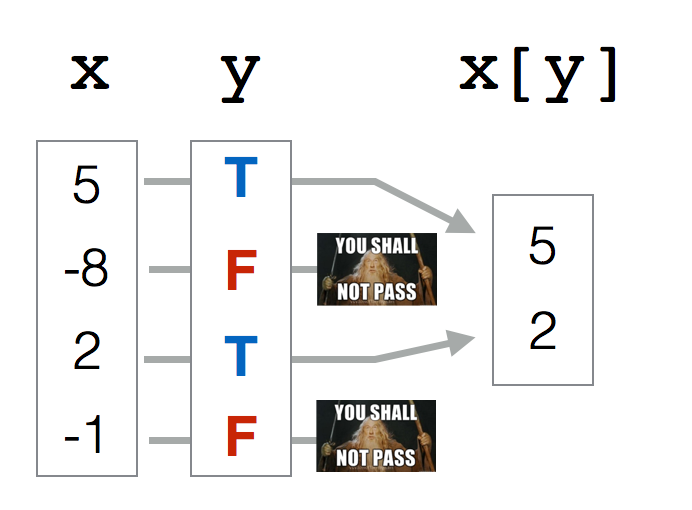
\includegraphics[width=4.16667in]{images/indexgandolf.png}
\caption{}
\end{figure}

Ну а если эти два вектора (исходный вектор и логический вектор индексов)
не равны по длине, то тут будет снова работать правило ресайклинга!

\begin{Shaded}
\begin{Highlighting}[]
\NormalTok{n[}\KeywordTok{c}\NormalTok{(}\OtherTok{TRUE}\NormalTok{, }\OtherTok{FALSE}\NormalTok{)] }\CommentTok{#то же самое - recycling rule!}
\end{Highlighting}
\end{Shaded}

\begin{verbatim}
## [1]  0 20  0  8 21
\end{verbatim}

Есть еще один способ индексирования векторов, но он несколько более
редкий: индексирование по имени. Дело в том, что для значений векторов
можно (но не обязательно) присваивать имена:

\begin{Shaded}
\begin{Highlighting}[]
\NormalTok{my_named_vector <-}\StringTok{ }\KeywordTok{c}\NormalTok{(}\DataTypeTok{first =} \DecValTok{1}\NormalTok{,}
                     \DataTypeTok{second =} \DecValTok{2}\NormalTok{,}
                     \DataTypeTok{third =} \DecValTok{3}\NormalTok{)}
\NormalTok{my_named_vector[}\StringTok{'first'}\NormalTok{]}
\end{Highlighting}
\end{Shaded}

\begin{verbatim}
## first 
##     1
\end{verbatim}

А еще можно ``вытаскивать'' имена из вектора с помощью функции
\texttt{names()} и присваивать таким образом новые имена.

\begin{Shaded}
\begin{Highlighting}[]
\NormalTok{d <-}\StringTok{ }\DecValTok{1}\OperatorTok{:}\DecValTok{4}
\KeywordTok{names}\NormalTok{(d) <-}\StringTok{ }\NormalTok{letters[}\DecValTok{1}\OperatorTok{:}\DecValTok{4}\NormalTok{]}
\KeywordTok{names}\NormalTok{(d)}
\end{Highlighting}
\end{Shaded}

\begin{verbatim}
## [1] "a" "b" "c" "d"
\end{verbatim}

\begin{Shaded}
\begin{Highlighting}[]
\NormalTok{d[}\StringTok{"a"}\NormalTok{]}
\end{Highlighting}
\end{Shaded}

\begin{verbatim}
## a 
## 1
\end{verbatim}

\begin{quote}
\texttt{letters} --- это ``зашитая'' в R константа --- вектор букв от a
до z. Иногда это очень удобно! Кроме того, есть константа
\texttt{LETTERS} --- то же самое, но заглавными буквами. А еще в R есть
названия месяцев на английском и числовая константа \texttt{pi}.
\end{quote}

Вернемся к нашему вектору \texttt{n} и посчитаем его среднее с помощью
функции \texttt{mean()}:

\begin{Shaded}
\begin{Highlighting}[]
\KeywordTok{mean}\NormalTok{(n)}
\end{Highlighting}
\end{Shaded}

\begin{verbatim}
## [1] 9.7
\end{verbatim}

А как вытащить все значения, которые больше среднего?

Сначала получим логический вектор --- какие значения больше среднего:

\begin{Shaded}
\begin{Highlighting}[]
\NormalTok{larger <-}\StringTok{ }\NormalTok{n}\OperatorTok{>}\KeywordTok{mean}\NormalTok{(n)}
\NormalTok{larger}
\end{Highlighting}
\end{Shaded}

\begin{verbatim}
##  [1] FALSE FALSE  TRUE FALSE FALSE FALSE FALSE  TRUE  TRUE  TRUE
\end{verbatim}

А теперь используем его для индексирования вектора \texttt{n}:

\begin{Shaded}
\begin{Highlighting}[]
\NormalTok{n[larger]}
\end{Highlighting}
\end{Shaded}

\begin{verbatim}
## [1] 20 13 21 34
\end{verbatim}

Можно все это сделать в одну строчку:

\begin{Shaded}
\begin{Highlighting}[]
\NormalTok{n[n}\OperatorTok{>}\KeywordTok{mean}\NormalTok{(n)]}
\end{Highlighting}
\end{Shaded}

\begin{verbatim}
## [1] 20 13 21 34
\end{verbatim}

Предыдущая строчка отражает то, что мы будем постоянно делать в R:
вычленять (subset) из данных отдельные куски на основании разных
условий.

\section{Работа с логическими векторами}\label{logic_vectors}

На работе с логическими векторами построено очень много удобных фишек,
связанных со сравнением условий.

\begin{Shaded}
\begin{Highlighting}[]
\NormalTok{eyes <-}\StringTok{ }\KeywordTok{c}\NormalTok{(}\StringTok{"green"}\NormalTok{, }\StringTok{"blue"}\NormalTok{, }\StringTok{"blue"}\NormalTok{, }\StringTok{"brown"}\NormalTok{, }\StringTok{"green"}\NormalTok{, }\StringTok{"blue"}\NormalTok{)}
\end{Highlighting}
\end{Shaded}

\subsection{\texorpdfstring{\texttt{mean()} и \texttt{sum()} для
подсчета пропорций и количества
TRUE}{mean() и sum() для подсчета пропорций и количества TRUE}}\label{logic_mean_sum}

Уже знакомая нам функция \texttt{sum()} позволяет посчитать количество
\texttt{TRUE} в логическом векторе. Например, можно удобно посчитать
сколько раз значение \texttt{"blue"} встречается в векторе
\texttt{eyes}:

\begin{Shaded}
\begin{Highlighting}[]
\NormalTok{eyes }\OperatorTok{==}\StringTok{ "blue"}
\end{Highlighting}
\end{Shaded}

\begin{verbatim}
## [1] FALSE  TRUE  TRUE FALSE FALSE  TRUE
\end{verbatim}

\begin{Shaded}
\begin{Highlighting}[]
\KeywordTok{sum}\NormalTok{(eyes }\OperatorTok{==}\StringTok{ "blue"}\NormalTok{)}
\end{Highlighting}
\end{Shaded}

\begin{verbatim}
## [1] 3
\end{verbatim}

Функцию \texttt{mean()} можно использовать для подсчета пропорций
\texttt{TRUE} в логическом векторе.

\begin{Shaded}
\begin{Highlighting}[]
\NormalTok{eyes }\OperatorTok{==}\StringTok{ "blue"}
\end{Highlighting}
\end{Shaded}

\begin{verbatim}
## [1] FALSE  TRUE  TRUE FALSE FALSE  TRUE
\end{verbatim}

\begin{Shaded}
\begin{Highlighting}[]
\KeywordTok{mean}\NormalTok{(eyes }\OperatorTok{==}\StringTok{ "blue"}\NormalTok{)}
\end{Highlighting}
\end{Shaded}

\begin{verbatim}
## [1] 0.5
\end{verbatim}

Умножив на 100, мы получим долю выраженную в процентах:

\begin{Shaded}
\begin{Highlighting}[]
\KeywordTok{mean}\NormalTok{(eyes }\OperatorTok{==}\StringTok{ "blue"}\NormalTok{) }\OperatorTok{*}\StringTok{ }\DecValTok{100}
\end{Highlighting}
\end{Shaded}

\begin{verbatim}
## [1] 50
\end{verbatim}

\subsection{\texorpdfstring{\texttt{all()} и
\texttt{any()}}{all() и any()}}\label{all_any}

Функция \texttt{all()} выдает \texttt{TRUE} только когда все значения
логического вектора на входе равны \texttt{TRUE}:

\begin{Shaded}
\begin{Highlighting}[]
\KeywordTok{all}\NormalTok{(eyes }\OperatorTok{==}\StringTok{ "blue"}\NormalTok{)}
\end{Highlighting}
\end{Shaded}

\begin{verbatim}
## [1] FALSE
\end{verbatim}

Функция \texttt{any()} выдает \texttt{TRUE} когда есть хотя бы одно
значение \texttt{TRUE}:

\begin{Shaded}
\begin{Highlighting}[]
\KeywordTok{any}\NormalTok{(eyes }\OperatorTok{==}\StringTok{ "blue"}\NormalTok{)}
\end{Highlighting}
\end{Shaded}

\begin{verbatim}
## [1] TRUE
\end{verbatim}

Вместе с оператором \texttt{!} можно получить много дополнительных
вариантов. Например, есть ли хотя бы один \texttt{FALSE} в векторе?

\begin{Shaded}
\begin{Highlighting}[]
\KeywordTok{any}\NormalTok{(}\OperatorTok{!}\NormalTok{eyes }\OperatorTok{==}\StringTok{ "blue"}\NormalTok{)}
\end{Highlighting}
\end{Shaded}

\begin{verbatim}
## [1] TRUE
\end{verbatim}

\begin{Shaded}
\begin{Highlighting}[]
\OperatorTok{!}\KeywordTok{all}\NormalTok{(eyes }\OperatorTok{==}\StringTok{ "blue"}\NormalTok{)}
\end{Highlighting}
\end{Shaded}

\begin{verbatim}
## [1] TRUE
\end{verbatim}

Все ли значения в векторе равны \texttt{FALSE}?

\begin{Shaded}
\begin{Highlighting}[]
\KeywordTok{all}\NormalTok{(}\OperatorTok{!}\NormalTok{eyes }\OperatorTok{==}\StringTok{ "blue"}\NormalTok{)}
\end{Highlighting}
\end{Shaded}

\begin{verbatim}
## [1] FALSE
\end{verbatim}

\begin{Shaded}
\begin{Highlighting}[]
\OperatorTok{!}\KeywordTok{any}\NormalTok{(eyes }\OperatorTok{==}\StringTok{ "blue"}\NormalTok{)}
\end{Highlighting}
\end{Shaded}

\begin{verbatim}
## [1] FALSE
\end{verbatim}

\subsection{\texorpdfstring{Превращение логических значений в индексы:
\texttt{which()}}{Превращение логических значений в индексы: which()}}\label{which}

Как вы уже знаете, и логические векторы, и числовые вектора с индексами
могут использоваться для индексирования векторов. Иногда может
понадобиться превратить логический вектор в вектор индексов. Для этого
есть функция \texttt{which()}

\begin{Shaded}
\begin{Highlighting}[]
\KeywordTok{which}\NormalTok{(eyes }\OperatorTok{==}\StringTok{ "blue"}\NormalTok{)}
\end{Highlighting}
\end{Shaded}

\begin{verbatim}
## [1] 2 3 6
\end{verbatim}

\subsection{оператор \%in\% и match()}\label{in}

Часто возникает такая задача: нужно проверить вектор на равенство с хотя
бы одним значением из другого вектора. Например, мы хотим вычленить всех
зеленоглазых и голубоглазых. Может возникнуть идея сделать так:

\begin{Shaded}
\begin{Highlighting}[]
\NormalTok{eyes[eyes }\OperatorTok{==}\StringTok{ }\KeywordTok{c}\NormalTok{(}\StringTok{"green"}\NormalTok{, }\StringTok{"blue"}\NormalTok{)]}
\end{Highlighting}
\end{Shaded}

\begin{verbatim}
## [1] "green" "blue"  "green" "blue"
\end{verbatim}

Перед нами самый страшный случай: результат \emph{похож} на правильный,
но не правильный! Попытайтесь самостоятельно понять почему этот ответ
неверный и что произошло на самом деле.

А на самом деле мы просто сравнили два вектора, один из которых короче
другого, следовательно, у нас сработало правило ресайклинга.

\begin{figure}
\centering
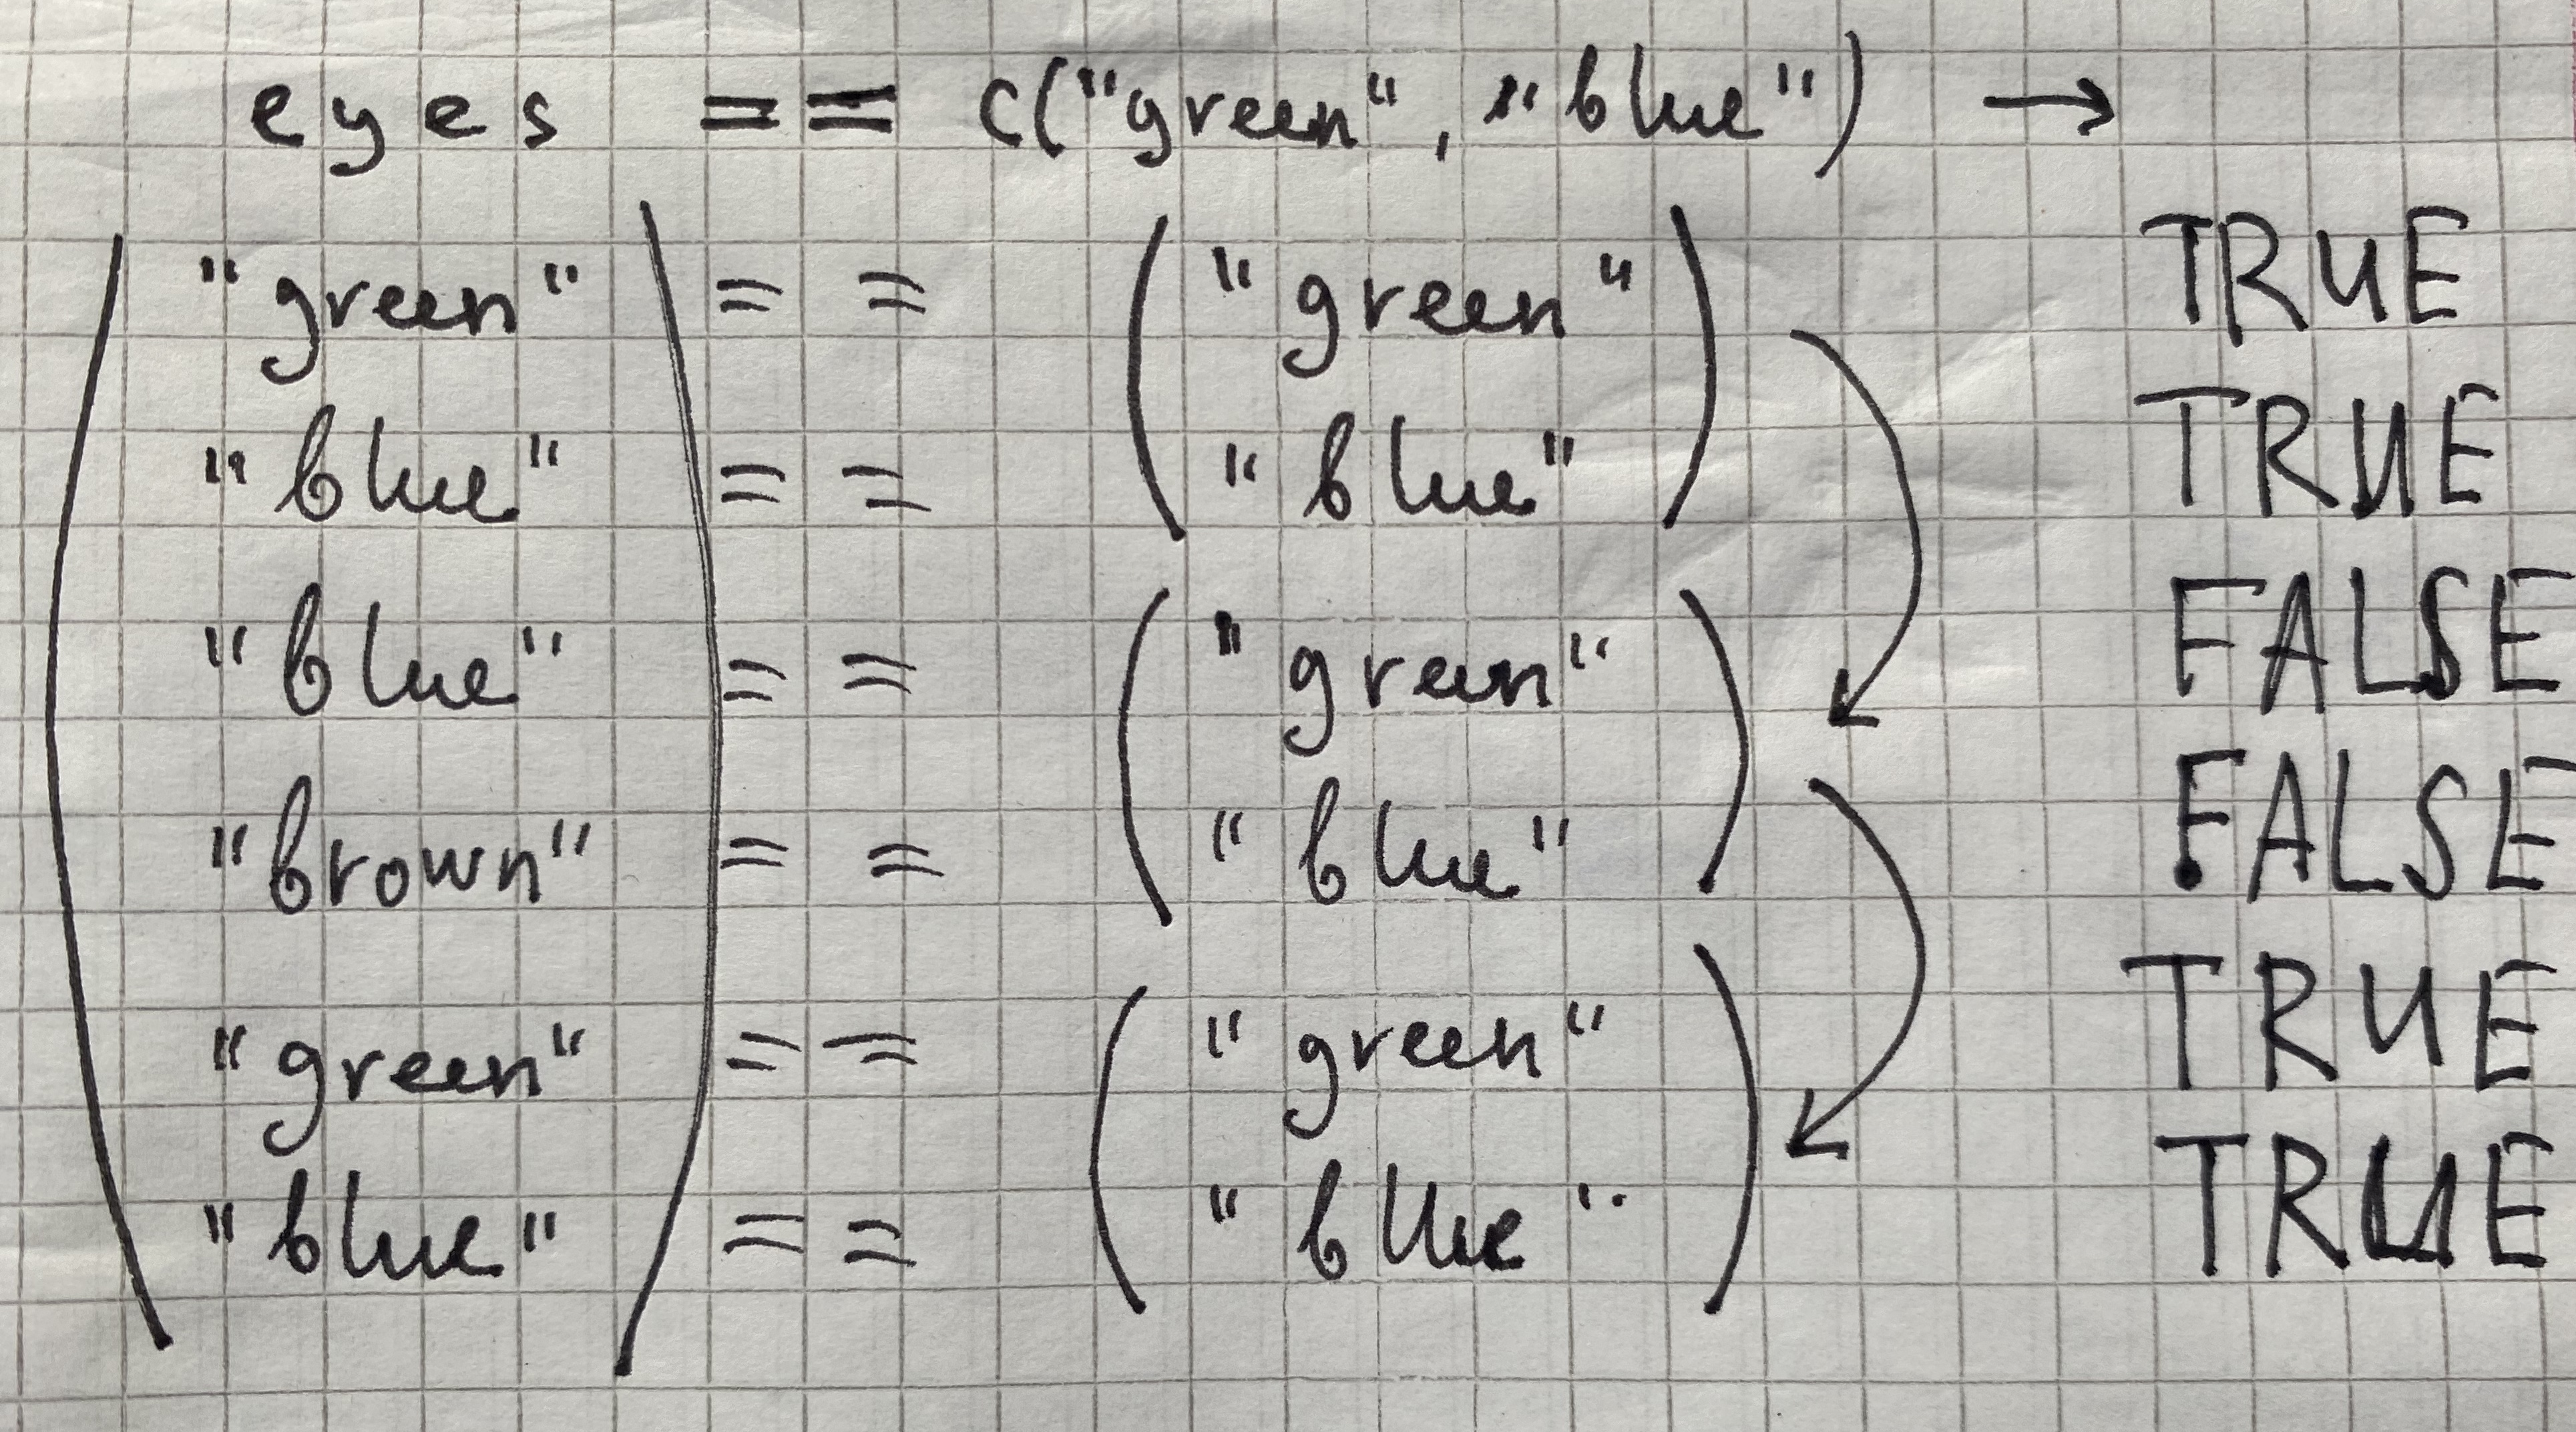
\includegraphics{images/logical_vectors_recycling.jpg}
\caption{}
\end{figure}

Как мы видим, это совсем не то, что нам нужно! В данной ситуации нам
подойдет сравнение с двумя значениями вместе с логическим ИЛИ.

\begin{Shaded}
\begin{Highlighting}[]
\NormalTok{eyes[eyes }\OperatorTok{==}\StringTok{ "green"} \OperatorTok{|}\StringTok{ }\NormalTok{eyes }\OperatorTok{==}\StringTok{ "blue"}\NormalTok{]}
\end{Highlighting}
\end{Shaded}

\begin{verbatim}
## [1] "green" "blue"  "blue"  "green" "blue"
\end{verbatim}

Однако это не очень удобно, особенно если значений больше 2. Тогда на
помощь приходит оператор \texttt{\%in\%}, который выполняет именно то,
что нам изначально нужно: выдает для каждого значения в векторе слева,
есть ли это значение среди значений вектора справа.

\begin{Shaded}
\begin{Highlighting}[]
\NormalTok{eyes[eyes }\OperatorTok\StringTok{ }\KeywordTok{c}\NormalTok{(}\StringTok{"green"}\NormalTok{, }\StringTok{"blue"}\NormalTok{)]}
\end{Highlighting}
\end{Shaded}

\begin{verbatim}
## [1] "green" "blue"  "blue"  "green" "blue"
\end{verbatim}

Основное преимущество оператора \texttt{\%in\%} в его простоте и
понятности. У оператора \texttt{\%in\%} есть старший брат, более сложный
и более мощный. Функция \texttt{match()} работает похожим образом на
\texttt{\%in\%}, но при совпадении значения в левом векторе с одним из
значений в правом выдает индекс соответствующего значения вместо
\texttt{TRUE}. Если же совпадений нет, то вместо \texttt{FALSE} функция
\texttt{match()} выдает \texttt{NA} (что можно поменять параметром
\texttt{nomatch\ =}).

\begin{Shaded}
\begin{Highlighting}[]
\KeywordTok{match}\NormalTok{(eyes, }\KeywordTok{c}\NormalTok{(}\StringTok{"green"}\NormalTok{, }\StringTok{"blue"}\NormalTok{))}
\end{Highlighting}
\end{Shaded}

\begin{verbatim}
## [1]  1  2  2 NA  1  2
\end{verbatim}

Зачем это может понадобиться? Во-первых, это способ соединить два набора
данных (хотя для этого есть и более подходящие инструменты), во-вторых,
можно так можно заменить все значения кроме выбранных заменить на
\texttt{NA}.

\begin{Shaded}
\begin{Highlighting}[]
\KeywordTok{c}\NormalTok{(}\StringTok{"green"}\NormalTok{, }\StringTok{"blue"}\NormalTok{)[}\KeywordTok{match}\NormalTok{(eyes, }\KeywordTok{c}\NormalTok{(}\StringTok{"green"}\NormalTok{, }\StringTok{"blue"}\NormalTok{))]}
\end{Highlighting}
\end{Shaded}

\begin{verbatim}
## [1] "green" "blue"  "blue"  NA      "green" "blue"
\end{verbatim}

\section{NA - пропущенные значения}\label{na}

В реальных данных у нас часто чего-то не хватает. Например, из-за
технической ошибки или невнимательности не получилось записать какое-то
измерение. Для обозначения пропущенных значений в R есть специальное
значение \texttt{NA} (расшифровывается как \emph{Not Available} -
недоступное значение). \texttt{NA} --- это не строка \texttt{"NA"}, не
\texttt{0}, не пустая строка \texttt{""} и не \texttt{FALSE}.
\texttt{NA} --- это \texttt{NA}. Большинство операций с векторами,
содержащими \texttt{NA} будут выдавать \texttt{NA}:

\begin{Shaded}
\begin{Highlighting}[]
\NormalTok{missed <-}\StringTok{ }\OtherTok{NA}
\NormalTok{missed }\OperatorTok{==}\StringTok{ "NA"}
\end{Highlighting}
\end{Shaded}

\begin{verbatim}
## [1] NA
\end{verbatim}

\begin{Shaded}
\begin{Highlighting}[]
\NormalTok{missed }\OperatorTok{==}\StringTok{ ""}
\end{Highlighting}
\end{Shaded}

\begin{verbatim}
## [1] NA
\end{verbatim}

\begin{Shaded}
\begin{Highlighting}[]
\NormalTok{missed }\OperatorTok{==}\StringTok{ }\OtherTok{NA}
\end{Highlighting}
\end{Shaded}

\begin{verbatim}
## [1] NA
\end{verbatim}

Заметьте, даже сравнение \texttt{NA} c \texttt{NA} выдает \texttt{NA}.
Это может прозвучать абсурдно: ну как же так, и то \texttt{NA}, и другое
\texttt{NA} --- это же одно и то же, они должны быть равны! Не совсем:
\texttt{NA} --- это отсутствие информации об объекте, неопределенность,
неизвестная нам величина. Если мы не знаем двух значений (т.е. имеем два
\texttt{NA}), то это еще не значит, что они равны.

Иногда наличие \texttt{NA} в данных очень бесит:

\begin{Shaded}
\begin{Highlighting}[]
\NormalTok{n[}\DecValTok{5}\NormalTok{] <-}\StringTok{ }\OtherTok{NA}
\NormalTok{n}
\end{Highlighting}
\end{Shaded}

\begin{verbatim}
##  [1]  0  1 20  0 NA  0  8 13 21 34
\end{verbatim}

\begin{Shaded}
\begin{Highlighting}[]
\KeywordTok{mean}\NormalTok{(n)}
\end{Highlighting}
\end{Shaded}

\begin{verbatim}
## [1] NA
\end{verbatim}

Получается, что наличие \texttt{NA} ``заражает'' неопределенностью все
последующие действия. Что же делать?\\
Наверное, надо сравнить вектор с \texttt{NA} и исключить этих
пакостников. Давайте попробуем:

\begin{Shaded}
\begin{Highlighting}[]
\NormalTok{n }\OperatorTok{==}\StringTok{ }\OtherTok{NA}
\end{Highlighting}
\end{Shaded}

\begin{verbatim}
##  [1] NA NA NA NA NA NA NA NA NA NA
\end{verbatim}

Ах да, мы ведь только что узнали, что даже сравнение \texttt{NA} c
\texttt{NA} приводит к \texttt{NA}!

Чтобы выбраться из этой непростой ситуации, используйте функцию
\texttt{is.na()}:

\begin{Shaded}
\begin{Highlighting}[]
\KeywordTok{is.na}\NormalTok{(n)}
\end{Highlighting}
\end{Shaded}

\begin{verbatim}
##  [1] FALSE FALSE FALSE FALSE  TRUE FALSE FALSE FALSE FALSE FALSE
\end{verbatim}

Результат выполнения \texttt{is.na(n)} выдает \texttt{FALSE} в тех
местах, где у нас числа и \texttt{TRUE} там, где у нас \texttt{NA}.
Чтобы вычленить из вектора \texttt{n} все значения кроме \texttt{NA} нам
нужно, чтобы было наоборот: \texttt{TRUE}, если это не \texttt{NA},
\texttt{FALSE}, если это \texttt{NA}. Здесь нам понадобится логический
оператор НЕ \texttt{!} (мы его уже встречали), который инвертирует
логические значения:

\begin{Shaded}
\begin{Highlighting}[]
\NormalTok{n[}\OperatorTok{!}\KeywordTok{is.na}\NormalTok{(n)]}
\end{Highlighting}
\end{Shaded}

\begin{verbatim}
## [1]  0  1 20  0  0  8 13 21 34
\end{verbatim}

Ура, мы можем считать среднее!

\begin{Shaded}
\begin{Highlighting}[]
\KeywordTok{mean}\NormalTok{(n[}\OperatorTok{!}\KeywordTok{is.na}\NormalTok{(n)])}
\end{Highlighting}
\end{Shaded}

\begin{verbatim}
## [1] 10.77778
\end{verbatim}

Теперь Вы понимаете, зачем нужно отрицание (\texttt{!})

Вообще, есть еще один из способов посчитать среднее, если есть
\texttt{NA}. Для этого надо залезть в хэлп по функции \emph{mean()}:

\begin{Shaded}
\begin{Highlighting}[]
\NormalTok{?}\KeywordTok{mean}\NormalTok{()}
\end{Highlighting}
\end{Shaded}

В хэлпе мы найдем параметр \texttt{na.rm\ =}, который по умолчанию
\texttt{FALSE}. Вы знаете, что нужно делать!

\begin{Shaded}
\begin{Highlighting}[]
\KeywordTok{mean}\NormalTok{(n, }\DataTypeTok{na.rm =}\NormalTok{ T)}
\end{Highlighting}
\end{Shaded}

\begin{verbatim}
## [1] 10.77778
\end{verbatim}

\begin{quote}
\texttt{NA} может появляться в векторах других типов тоже. На самом
деле, \texttt{NA} - это специальное значение в логических векторах,
тогда как в векторах других типов \texttt{NA} появляется как
\texttt{NA\_integer\_}, \texttt{NA\_real\_}, \texttt{NA\_complex\_} или
\texttt{NA\_character\_}, но R обычно сам все переводит в нужный формат
и показывает как просто \texttt{NA}.
\end{quote}

\begin{quote}
Кроме \texttt{NA} есть еще \texttt{NaN} --- это разные вещи.
\texttt{NaN} расшифровывается как \emph{Not a Number} и получается в
результате таких операций как \texttt{0\ /\ 0}. Тем не менее, функция
\texttt{is.na()} выдает \texttt{TRUE} на \texttt{NaN}, а вот функция
\texttt{is.nan()} выдает \texttt{TRUE} на \texttt{NaN} и \texttt{FALSE}
на \texttt{NA}:
\end{quote}

\begin{Shaded}
\begin{Highlighting}[]
\KeywordTok{is.na}\NormalTok{(}\OtherTok{NA}\NormalTok{)}
\end{Highlighting}
\end{Shaded}

\begin{verbatim}
## [1] TRUE
\end{verbatim}

\begin{Shaded}
\begin{Highlighting}[]
\KeywordTok{is.na}\NormalTok{(}\OtherTok{NaN}\NormalTok{)}
\end{Highlighting}
\end{Shaded}

\begin{verbatim}
## [1] TRUE
\end{verbatim}

\begin{Shaded}
\begin{Highlighting}[]
\KeywordTok{is.nan}\NormalTok{(}\OtherTok{NA}\NormalTok{)}
\end{Highlighting}
\end{Shaded}

\begin{verbatim}
## [1] FALSE
\end{verbatim}

\begin{Shaded}
\begin{Highlighting}[]
\KeywordTok{is.nan}\NormalTok{(}\OtherTok{NaN}\NormalTok{)}
\end{Highlighting}
\end{Shaded}

\begin{verbatim}
## [1] TRUE
\end{verbatim}

\section{Заключение}\label{vector_end}

Итак, с векторами мы более-менее разобрались. Помните, что вектора ---
это один из краеугольных камней вашей работы в R. Если вы хорошо с ними
разобрались, то дальше все будет довольно несложно. Тем не менее,
вектора --- это не все. Есть еще два важных типа данных: списки
(\textbf{list}) и матрицы (\textbf{matrix}). Их можно рассматривать как
своеобразное ``расширение'' векторов, каждый в свою сторону. Ну а списки
и матрицы нужны чтобы понять основной тип данных в R ---
\textbf{data.frame}.

\begin{figure}
\centering
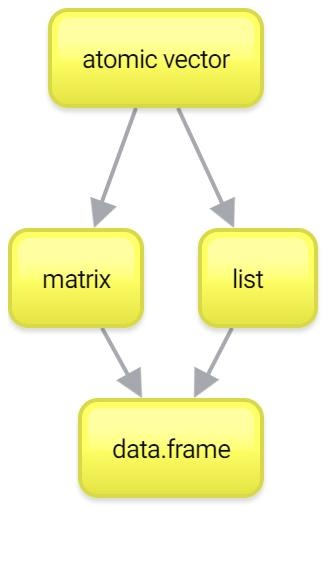
\includegraphics[width=4.16667in]{images/New-Mind-Map.jpg}
\caption{}
\end{figure}

\chapter{Сложные структуры данных в R}\label{complex_structures}

\section{Матрица}\label{matrix}

Если вдруг вас пугает это слово, то совершенно зря. \textbf{Матрица
(matrix)} --- это всего лишь ``двумерный'' вектор: вектор, у которого
есть не только длина, но и ширина. Создать матрицу можно с помощью
функции \texttt{matrix()} из вектора, указав при этом количество строк и
столбцов.

\begin{Shaded}
\begin{Highlighting}[]
\NormalTok{A <-}\StringTok{ }\KeywordTok{matrix}\NormalTok{(}\DecValTok{1}\OperatorTok{:}\DecValTok{20}\NormalTok{, }\DataTypeTok{nrow=}\DecValTok{5}\NormalTok{,}\DataTypeTok{ncol=}\DecValTok{4}\NormalTok{)}
\NormalTok{A}
\end{Highlighting}
\end{Shaded}

\begin{verbatim}
##      [,1] [,2] [,3] [,4]
## [1,]    1    6   11   16
## [2,]    2    7   12   17
## [3,]    3    8   13   18
## [4,]    4    9   14   19
## [5,]    5   10   15   20
\end{verbatim}

\begin{quote}
Заметьте, значения вектора заполняются следующим образом: сначала
заполняется первый столбик сверху вниз, потом второй сверху вниз и так
до конца, т.е. заполнение значений матрицы идет в первую очередь по
вертикали. Это довольно стандартный способ создания матриц, характерный
не только для R.
\end{quote}

Если мы знаем сколько значений в матрице и сколько мы хотим строк, то
количество столбцов указывать необязательно:

\begin{Shaded}
\begin{Highlighting}[]
\NormalTok{A <-}\StringTok{ }\KeywordTok{matrix}\NormalTok{(}\DecValTok{1}\OperatorTok{:}\DecValTok{20}\NormalTok{, }\DataTypeTok{nrow=}\DecValTok{5}\NormalTok{)}
\NormalTok{A}
\end{Highlighting}
\end{Shaded}

\begin{verbatim}
##      [,1] [,2] [,3] [,4]
## [1,]    1    6   11   16
## [2,]    2    7   12   17
## [3,]    3    8   13   18
## [4,]    4    9   14   19
## [5,]    5   10   15   20
\end{verbatim}

Все остальное так же как и с векторами: внутри находится данные только
одного типа. Поскольку матрица --- это уже двумерный массив, то у него
имеется два индекса. Эти два индекса разделяются запятыми.

\begin{Shaded}
\begin{Highlighting}[]
\NormalTok{A[}\DecValTok{2}\NormalTok{,}\DecValTok{3}\NormalTok{]}
\end{Highlighting}
\end{Shaded}

\begin{verbatim}
## [1] 12
\end{verbatim}

\begin{Shaded}
\begin{Highlighting}[]
\NormalTok{A[}\DecValTok{2}\OperatorTok{:}\DecValTok{4}\NormalTok{, }\DecValTok{1}\OperatorTok{:}\DecValTok{3}\NormalTok{]}
\end{Highlighting}
\end{Shaded}

\begin{verbatim}
##      [,1] [,2] [,3]
## [1,]    2    7   12
## [2,]    3    8   13
## [3,]    4    9   14
\end{verbatim}

Первый индекс --- выбор строк, второй индекс --- выбор колонок. Если же
мы оставляем пустое поле вместо числа, то мы выбираем все строки/колонки
в зависимости от того, оставили мы поле пустым до или после запятой:

\begin{Shaded}
\begin{Highlighting}[]
\NormalTok{A[, }\DecValTok{1}\OperatorTok{:}\DecValTok{3}\NormalTok{]}
\end{Highlighting}
\end{Shaded}

\begin{verbatim}
##      [,1] [,2] [,3]
## [1,]    1    6   11
## [2,]    2    7   12
## [3,]    3    8   13
## [4,]    4    9   14
## [5,]    5   10   15
\end{verbatim}

\begin{Shaded}
\begin{Highlighting}[]
\NormalTok{A[}\DecValTok{2}\OperatorTok{:}\DecValTok{4}\NormalTok{, ]}
\end{Highlighting}
\end{Shaded}

\begin{verbatim}
##      [,1] [,2] [,3] [,4]
## [1,]    2    7   12   17
## [2,]    3    8   13   18
## [3,]    4    9   14   19
\end{verbatim}

\begin{Shaded}
\begin{Highlighting}[]
\NormalTok{A[, ]}
\end{Highlighting}
\end{Shaded}

\begin{verbatim}
##      [,1] [,2] [,3] [,4]
## [1,]    1    6   11   16
## [2,]    2    7   12   17
## [3,]    3    8   13   18
## [4,]    4    9   14   19
## [5,]    5   10   15   20
\end{verbatim}

Так же как и в случае с обычными векторами, часть матрицы можно
переписать:

\begin{Shaded}
\begin{Highlighting}[]
\NormalTok{A[}\DecValTok{2}\OperatorTok{:}\DecValTok{4}\NormalTok{, }\DecValTok{2}\OperatorTok{:}\DecValTok{4}\NormalTok{] <-}\StringTok{ }\DecValTok{100}
\NormalTok{A}
\end{Highlighting}
\end{Shaded}

\begin{verbatim}
##      [,1] [,2] [,3] [,4]
## [1,]    1    6   11   16
## [2,]    2  100  100  100
## [3,]    3  100  100  100
## [4,]    4  100  100  100
## [5,]    5   10   15   20
\end{verbatim}

В принципе, это все, что нам нужно знать о матрицах. Матрицы
используются в R довольно редко, особенно по сравнению, например, с
MATLAB. Но вот индексировать матрицы хорошо бы уметь: это понадобится в
работе с датафреймами.

\begin{quote}
То, что матрица --- это просто двумерный вектор, не является метафорой:
в R матрица --- это по сути своей вектор с дополнительными
\emph{атрибутами} \texttt{dim} и (опционально) \texttt{dimnames}.
Атрибуты --- это свойства объектов, своего рода ``метаданные''. Для всех
объектов есть обязательные атрибуты типа и длины и могут быть любые
необязательные атрибуты. Можно задавать свои атрибуты или удалять уже
присвоенные: удаление атрибута \texttt{dim} у матрицы превратит ее в
обычный вектор. Про атрибуты подробнее можно почитать
\href{https://perso.esiee.fr/~courivad/R/06-objects.html}{здесь} или на
стр. 99-101 книги ``R in a Nutshell'' \citep{adler2010r}.
\end{quote}

\section{Массив}\label{arrays}

Два измерения --- это не предел! Структура с одним типом данных внутри,
но с тремя измерениями или больше, называется \textbf{массивом (array)}.
Создание массива очень похоже на создание матрицы: задаем вектор, из
которого будет собран массив, и размерность массива.

\begin{Shaded}
\begin{Highlighting}[]
\NormalTok{array_3d <-}\StringTok{ }\KeywordTok{array}\NormalTok{(}\DecValTok{1}\OperatorTok{:}\DecValTok{12}\NormalTok{, }\KeywordTok{c}\NormalTok{(}\DecValTok{3}\NormalTok{, }\DecValTok{2}\NormalTok{, }\DecValTok{2}\NormalTok{))}
\NormalTok{array_3d}
\end{Highlighting}
\end{Shaded}

\begin{verbatim}
## , , 1
## 
##      [,1] [,2]
## [1,]    1    4
## [2,]    2    5
## [3,]    3    6
## 
## , , 2
## 
##      [,1] [,2]
## [1,]    7   10
## [2,]    8   11
## [3,]    9   12
\end{verbatim}

\section{Список}\label{list}

Теперь представим себе вектор без ограничения на одинаковые данные
внутри. И получим \textbf{список (list)}!

\begin{Shaded}
\begin{Highlighting}[]
\NormalTok{simple_list <-}\StringTok{ }\KeywordTok{list}\NormalTok{(}\DecValTok{42}\NormalTok{, }\StringTok{"Пам пам"}\NormalTok{, }\OtherTok{TRUE}\NormalTok{)}
\NormalTok{simple_list}
\end{Highlighting}
\end{Shaded}

\begin{verbatim}
## [[1]]
## [1] 42
## 
## [[2]]
## [1] "Пам пам"
## 
## [[3]]
## [1] TRUE
\end{verbatim}

А это значит, что там могут содержаться самые разные данные, в том числе
и другие списки и векторы!

\begin{Shaded}
\begin{Highlighting}[]
\NormalTok{complex_list <-}\StringTok{ }\KeywordTok{list}\NormalTok{(}\KeywordTok{c}\NormalTok{(}\StringTok{"Wow"}\NormalTok{, }\StringTok{"this"}\NormalTok{, }\StringTok{"list"}\NormalTok{, }\StringTok{"is"}\NormalTok{, }\StringTok{"so"}\NormalTok{, }\StringTok{"big"}\NormalTok{), }\StringTok{"16"}\NormalTok{, simple_list)}
\NormalTok{complex_list}
\end{Highlighting}
\end{Shaded}

\begin{verbatim}
## [[1]]
## [1] "Wow"  "this" "list" "is"   "so"   "big" 
## 
## [[2]]
## [1] "16"
## 
## [[3]]
## [[3]][[1]]
## [1] 42
## 
## [[3]][[2]]
## [1] "Пам пам"
## 
## [[3]][[3]]
## [1] TRUE
\end{verbatim}

Если у нас сложный список, то есть очень классная функция, чтобы
посмотреть, как он устроен, под названием \texttt{str()}:

\begin{Shaded}
\begin{Highlighting}[]
\KeywordTok{str}\NormalTok{(complex_list)}
\end{Highlighting}
\end{Shaded}

\begin{verbatim}
## List of 3
##  $ : chr [1:6] "Wow" "this" "list" "is" ...
##  $ : chr "16"
##  $ :List of 3
##   ..$ : num 42
##   ..$ : chr "Пам пам"
##   ..$ : logi TRUE
\end{verbatim}

\begin{quote}
Представьте, что список - это такое дерево с ветвистой структурой. А на
конце этих ветвей - листья-векторы.
\end{quote}

Как и в случае с векторами мы можем давать имена элементам списка:

\begin{Shaded}
\begin{Highlighting}[]
\NormalTok{named_list <-}\StringTok{ }\KeywordTok{list}\NormalTok{(}\DataTypeTok{age =} \DecValTok{24}\NormalTok{, }\DataTypeTok{PhDstudent =}\NormalTok{ T, }\DataTypeTok{language =} \StringTok{"Russian"}\NormalTok{)}
\NormalTok{named_list}
\end{Highlighting}
\end{Shaded}

\begin{verbatim}
## $age
## [1] 24
## 
## $PhDstudent
## [1] TRUE
## 
## $language
## [1] "Russian"
\end{verbatim}

К списку можно обращаться как с помощью индексов, так и по именам.
Начнем с последнего:

\begin{Shaded}
\begin{Highlighting}[]
\NormalTok{named_list}\OperatorTok{$}\NormalTok{age}
\end{Highlighting}
\end{Shaded}

\begin{verbatim}
## [1] 24
\end{verbatim}

А вот с индексами сложнее, и в этом очень легко запутаться. Давайте
попробуем сделать так, как мы делали это раньше:

\begin{Shaded}
\begin{Highlighting}[]
\NormalTok{named_list[}\DecValTok{1}\NormalTok{]}
\end{Highlighting}
\end{Shaded}

\begin{verbatim}
## $age
## [1] 24
\end{verbatim}

Мы, по сути, получили элемент списка --- просто как часть списка, т.е.
как список длиной один:

\begin{Shaded}
\begin{Highlighting}[]
\KeywordTok{class}\NormalTok{(named_list)}
\end{Highlighting}
\end{Shaded}

\begin{verbatim}
## [1] "list"
\end{verbatim}

\begin{Shaded}
\begin{Highlighting}[]
\KeywordTok{class}\NormalTok{(named_list[}\DecValTok{1}\NormalTok{])}
\end{Highlighting}
\end{Shaded}

\begin{verbatim}
## [1] "list"
\end{verbatim}

А вот чтобы добраться до самого элемента списка (и сделать с ним что-то
хорошее), нам нужна не одна, а две квадратных скобочки:

\begin{Shaded}
\begin{Highlighting}[]
\NormalTok{named_list[[}\DecValTok{1}\NormalTok{]]}
\end{Highlighting}
\end{Shaded}

\begin{verbatim}
## [1] 24
\end{verbatim}

\begin{Shaded}
\begin{Highlighting}[]
\KeywordTok{class}\NormalTok{(named_list[[}\DecValTok{1}\NormalTok{]])}
\end{Highlighting}
\end{Shaded}

\begin{verbatim}
## [1] "numeric"
\end{verbatim}

Indexing lists in \#rstats. Inspired by the Residence Inn
pic.twitter.com/YQ6axb2w7t

--- Hadley Wickham (\citet{hadleywickham}) September 14, 2015

Как и в случае с вектором, к элементу списка можно обращаться по имени.

\begin{Shaded}
\begin{Highlighting}[]
\NormalTok{named_list[[}\StringTok{'age'}\NormalTok{]]}
\end{Highlighting}
\end{Shaded}

\begin{verbatim}
## [1] 24
\end{verbatim}

Хотя последнее --- практически то же самое, что и использование знака
\$.

\begin{quote}
Списки довольно часто используются в R, но реже, чем в Python. Со
многими объектами в R, такими как результаты статистических тестов,
удобно работать именно как со списками --- к ним все вышеописанное
применимо. Кроме того, некоторые данные мы изначально получаем в виде
древообразной структуры --- хочешь не хочешь, а придется работать с этим
как со списком. Но обычно после этого стоит как можно скорее превратить
список в датафрейм.
\end{quote}

\section{Датафрейм}\label{df}

Итак, мы перешли к самому главному. Самому-самому. \textbf{Датафреймы
(data.frames)}. Более того, сейчас станет понятно, зачем нам нужно было
разбираться со всеми предыдущими темами.

Без векторов мы не смогли бы разобраться с матрицами и списками. А без
последних мы не сможем понять, что такое датафрейм.

\begin{Shaded}
\begin{Highlighting}[]
\NormalTok{name <-}\StringTok{ }\KeywordTok{c}\NormalTok{(}\StringTok{"Ivan"}\NormalTok{, }\StringTok{"Eugeny"}\NormalTok{, }\StringTok{"Lena"}\NormalTok{, }\StringTok{"Misha"}\NormalTok{, }\StringTok{"Sasha"}\NormalTok{) }
\NormalTok{age <-}\StringTok{ }\KeywordTok{c}\NormalTok{(}\DecValTok{26}\NormalTok{, }\DecValTok{34}\NormalTok{, }\DecValTok{23}\NormalTok{, }\DecValTok{27}\NormalTok{, }\DecValTok{26}\NormalTok{) }
\NormalTok{student <-}\StringTok{ }\KeywordTok{c}\NormalTok{(F, F, T, T, T) }
\NormalTok{df <-}\StringTok{ }\KeywordTok{data.frame}\NormalTok{(name, age, student)  }
\NormalTok{df}
\end{Highlighting}
\end{Shaded}

\begin{verbatim}
##     name age student
## 1   Ivan  26   FALSE
## 2 Eugeny  34   FALSE
## 3   Lena  23    TRUE
## 4  Misha  27    TRUE
## 5  Sasha  26    TRUE
\end{verbatim}

\begin{Shaded}
\begin{Highlighting}[]
\KeywordTok{str}\NormalTok{(df)}
\end{Highlighting}
\end{Shaded}

\begin{verbatim}
## 'data.frame':    5 obs. of  3 variables:
##  $ name   : chr  "Ivan" "Eugeny" "Lena" "Misha" ...
##  $ age    : num  26 34 23 27 26
##  $ student: logi  FALSE FALSE TRUE TRUE TRUE
\end{verbatim}

Вообще, очень похоже на список, не правда ли? Так и есть, датафрейм ---
это что-то вроде проименованного списка, каждый элемент которого
является \emph{atomic} вектором фиксированной длины. Скорее всего,
список Вы представляли ``горизонтально''. Если это так, то теперь
``переверните'' его у себя в голове на 90 градусов. Так, чтоб названия
векторов оказались сверху, а колонки стали столбцами. Поскольку длина
всех этих векторов равна (обязательное условие!), то данные представляют
собой табличку, похожую на матрицу. Но в отличие от матрицы, разные
столбцы могут имет разные типы данных. В нашем случае первая колонка ---
\texttt{character}, вторая колонка --- \texttt{numeric}, третья колонка
--- \texttt{logical}. Тем не менее, обращаться с датафреймом можно и как
с проименованным списком, и как с матрицей:

\begin{Shaded}
\begin{Highlighting}[]
\NormalTok{df}\OperatorTok{$}\NormalTok{age[}\DecValTok{2}\OperatorTok{:}\DecValTok{3}\NormalTok{]}
\end{Highlighting}
\end{Shaded}

\begin{verbatim}
## [1] 34 23
\end{verbatim}

Здесь мы сначала вытащили колонку \texttt{age} с помощью оператора
\texttt{\$}. Результатом этой операции является числовой вектор, из
которого мы вытащили кусок, выбрав индексы \texttt{2} и \texttt{3}.

Используя оператор \texttt{\$} и присваивание можно создавать новые
колонки датафрейма:

\begin{Shaded}
\begin{Highlighting}[]
\NormalTok{df}\OperatorTok{$}\NormalTok{lovesR <-}\StringTok{ }\NormalTok{T }\CommentTok{#правило recycling - узнали? }
\NormalTok{df}
\end{Highlighting}
\end{Shaded}

\begin{verbatim}
##     name age student lovesR
## 1   Ivan  26   FALSE   TRUE
## 2 Eugeny  34   FALSE   TRUE
## 3   Lena  23    TRUE   TRUE
## 4  Misha  27    TRUE   TRUE
## 5  Sasha  26    TRUE   TRUE
\end{verbatim}

Ну а можно просто обращаться с помощью двух индексов через запятую, как
мы это делали с матрицей:

\begin{Shaded}
\begin{Highlighting}[]
\NormalTok{df[}\DecValTok{3}\OperatorTok{:}\DecValTok{5}\NormalTok{, }\DecValTok{2}\OperatorTok{:}\DecValTok{3}\NormalTok{]}
\end{Highlighting}
\end{Shaded}

\begin{verbatim}
##   age student
## 3  23    TRUE
## 4  27    TRUE
## 5  26    TRUE
\end{verbatim}

Как и с матрицами, первый индекс означает строчки, а второй --- столбцы.

А еще можно использовать названия колонок внутри квадратных скобок:

\begin{Shaded}
\begin{Highlighting}[]
\NormalTok{df[}\DecValTok{1}\OperatorTok{:}\DecValTok{2}\NormalTok{,}\StringTok{"age"}\NormalTok{]}
\end{Highlighting}
\end{Shaded}

\begin{verbatim}
## [1] 26 34
\end{verbatim}

И здесь перед нами открываются невообразимые возможности! Узнаем, любят
ли R те, кто моложе среднего возраста в группе:

\begin{Shaded}
\begin{Highlighting}[]
\NormalTok{df[df}\OperatorTok{$}\NormalTok{age }\OperatorTok{<}\StringTok{ }\KeywordTok{mean}\NormalTok{(df}\OperatorTok{$}\NormalTok{age), }\DecValTok{4}\NormalTok{]}
\end{Highlighting}
\end{Shaded}

\begin{verbatim}
## [1] TRUE TRUE TRUE TRUE
\end{verbatim}

Эту же задачу можно выполнить другими способами:

\begin{Shaded}
\begin{Highlighting}[]
\NormalTok{df}\OperatorTok{$}\NormalTok{lovesR[df}\OperatorTok{$}\NormalTok{age }\OperatorTok{<}\StringTok{ }\KeywordTok{mean}\NormalTok{(df}\OperatorTok{$}\NormalTok{age)]}
\end{Highlighting}
\end{Shaded}

\begin{verbatim}
## [1] TRUE TRUE TRUE TRUE
\end{verbatim}

\begin{Shaded}
\begin{Highlighting}[]
\NormalTok{df[df}\OperatorTok{$}\NormalTok{age }\OperatorTok{<}\StringTok{ }\KeywordTok{mean}\NormalTok{(df}\OperatorTok{$}\NormalTok{age), }\StringTok{'lovesR'}\NormalTok{]}
\end{Highlighting}
\end{Shaded}

\begin{verbatim}
## [1] TRUE TRUE TRUE TRUE
\end{verbatim}

В большинстве случаев подходят сразу несколько способов --- тем не
менее, стоит овладеть ими всеми.

Датафреймы удобно просматривать в RStudio. Для это нужно написать
команду \texttt{View(df)} или же просто нажать на названии нужной
переменной из списка вверху справа (там где Environment). Тогда увидите
табличку, очень похожую на Excel и тому подобные программы для работы с
таблицами. Там же есть и всякие возможности для фильтрации, сортировки и
поиска\ldots{}\footnote{Все, что вы нажмете в этом окошке, никак не
  повлияет на исходную переменную. Так что можете смело использовать эти
  функции для исследования содержимого датафрейма.}

\begin{figure}
\centering
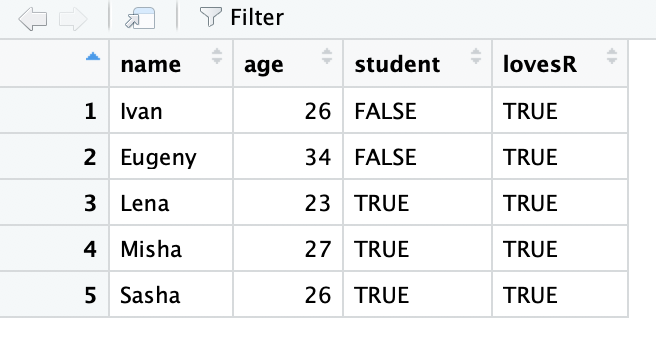
\includegraphics[width=2.08333in]{images/View.png}
\caption{}
\end{figure}

Но, конечно, интереснее все эти вещи делать руками, т.е. с помощью
написания кода.

\chapter{Пакеты в R}\label{r_packages}

\section{Дополнительные пакеты}\label{extra_pack}

R --- очень богатый язык с широкими возможностями. Однако очень скоро мы
поймем, что этих возможностей нам не хватает. Эти возможности нам могут
предоставить дополнительные \textbf{пакеты (packages)}.

В большинстве случаев основным содержанием пакетов является набор
дополнительных функций. Кроме функций, пакеты могут содержать наборы
данных и новые структуры данных.

Обычно пакеты посвящены решению какого-то класса задач в определенной
области. Например, есть множество пакетов для создания какого-то одного
типа визуализации. Еще один пример --- пакет \texttt{beepr}, который
содержит всего две функции: \texttt{beep()} и \texttt{beep\_on\_error()}
для воспроизведения звукового сигнала. Это может быть удобно, если ваш
скрипт работает долго, но вы хотите получить уведомление, когда его
выполнение завершится.

Более крупные пакеты посвящены целому классу задач. Например, пакеты
\texttt{stringi} и \texttt{stringr} посвящены работе со строками,
значительно расширяя и делая более удобной работу со строковыми данными
в R. Еще один пример: пакет \texttt{igraph} для работы с графами
(сетями). Этот пакет предоставляет дополнительный класс данных
\texttt{igraph} для хранения и работы с сетями.

Есть и совсем крупные пакеты, которые значительно расширяют базовый
функционал R, изменяя основные принципы работы в нем. Это пакеты
\texttt{data.table} и \texttt{tidyverse}. Это настолько крупные пакеты,
что их даже называют отдельными диалектами R, потому что код, написанный
с использованием этих пакетов, довольно сильно отличается от базового R.
Кроме того, \texttt{tidyverse} - это не просто пакет, а целая экосистема
пакетов, который взаимодополняют друг друга, но для удобства их можно
устанавливать и загружать как один пакет \texttt{tidyverse}. Еще один
пример крупной экосистемы из пакетов --- это пакет \texttt{mlr3} для
машинного обучения, который представляет собой большой расширяемый
``пакет пакетов'', где отдельные пакеты посвящены отдельным этапам и
задачам машинного обучения.

\section{Встроенные пакеты R}\label{r_built_in}

Вообще, даже сам R является набором из нескольких пакетов: основного
\texttt{base} и нескольких других, таких как \texttt{stats},
\texttt{utils}, \texttt{graphics}. Вот их полный список:

\begin{Shaded}
\begin{Highlighting}[]
\KeywordTok{rownames}\NormalTok{(}\KeywordTok{installed.packages}\NormalTok{(}\DataTypeTok{priority =} \StringTok{"base"}\NormalTok{))}
\end{Highlighting}
\end{Shaded}

\begin{verbatim}
##  [1] "base"      "compiler"  "datasets"  "graphics"  "grDevices" "grid"     
##  [7] "methods"   "parallel"  "splines"   "stats"     "stats4"    "tcltk"    
## [13] "tools"     "utils"
\end{verbatim}

Чтобы пользоваться этими пакетами ничего дополнительно делать не нужно.

\section{Установка пакетов с CRAN}\label{install_cran}

Функция \texttt{install.packages()} позволяет скачивать пакеты с
Comprehensive R Archive Network (CRAN). На репозитории CRAN собрано
более 16000 пакетов. Каждый из этих пакетов проходит проверку перед
попаданием в CRAN: он должен быть хорошо задокументирован, стабильно
работать и решать какую-то задачу.

Для примера установим пакет \texttt{remotes}. Это пакет для удобной
установки пакетов не с CRAN и скоро нам понадобится.

\begin{Shaded}
\begin{Highlighting}[]
\KeywordTok{install.packages}\NormalTok{(}\StringTok{"remotes"}\NormalTok{)}
\end{Highlighting}
\end{Shaded}

При установке вы увидите много непонятных надписей красным шрифтом. Не
пугайтесь, это нормально, происходит скачивание и установка пакетов. В
конце вы увидите что-то вроде этого:

!(){images/install\_success.png}

Иногда установка бывает очень долгой, потому что большие пакеты склонны
иметь много \textbf{зависимостей}: для работы какого-то пакета может
понадобиться другие пакеты, а для тех пакетов - еще какие-то пакеты.
Таким образом, устанавливая какой-нибудь современный пакет, вы,
возможно, установите десятки других пакетов! Зато если они понадобятся
сами по себе, то их уже не нужно будет устанавливать.

\section{Загрузка установленного пакета}\label{package_load}

Установить пакет с помощью \texttt{install.packages()} недостаточно,
пакет нужно еще загрузить. Для этого есть функция \texttt{library()}.

\begin{Shaded}
\begin{Highlighting}[]
\KeywordTok{library}\NormalTok{(}\StringTok{"remotes"}\NormalTok{)}
\end{Highlighting}
\end{Shaded}

В отличие от \texttt{install.packages()}, функция \texttt{library()}
принимает название пакета и как строчку в кавычках, и как название без
кавычек.

\begin{Shaded}
\begin{Highlighting}[]
\KeywordTok{library}\NormalTok{(remotes)}
\end{Highlighting}
\end{Shaded}

Теперь функции, данные и классы из пакета доступны для работы.

\section{\texorpdfstring{Вызов функции из пакета с помощью
\texttt{::}}{Вызов функции из пакета с помощью ::}}\label{from_package}

Если пакетом нужно воспользоваться всего один-два раза, то имеет смысл
не подключать весь пакет, а загрузить отдельную функцию из него. Для
этого есть специальный оператор \texttt{::}, который использует функцию
(указанную справа от \texttt{::}) из выбранного пакета (указанного слева
от \texttt{::}), не загружая пакет полностью.

Для примера воспользуемся функцией \texttt{package\_deps()} из только
что установленного пакета \texttt{remotes}, которая возвращает все
зависимости пакета:

\begin{Shaded}
\begin{Highlighting}[]
\NormalTok{remotes}\OperatorTok{::}\KeywordTok{package_deps}\NormalTok{(}\StringTok{"tidyverse"}\NormalTok{)}
\end{Highlighting}
\end{Shaded}

В дальнейшем использование оператора \texttt{::} будет иногда
использоваться, чтобы указать, из какого пакета взята функция.

Оператор \texttt{::} полезен еще и в тех случаях, когда в разных пакетах
присутствуют функции с одинаковым названием. Например, у основного
пакета tidyverse, \texttt{dplyr}, есть функция \texttt{filter()}.
Функция с точно таким же названием есть в базовом R в пакете
\texttt{stats}, в котором та выполняет совершенно другую задачу. Если у
вас уже загружен \texttt{dplyr}, то использование \texttt{::} укажет на
то, что вы хотите воспользоваться именно функцией \texttt{filter()} из
пакета \texttt{stats}:

\begin{Shaded}
\begin{Highlighting}[]
\NormalTok{stats}\OperatorTok{::}\KeywordTok{filter}\NormalTok{(}\DecValTok{1}\OperatorTok{:}\DecValTok{20}\NormalTok{, }\KeywordTok{rep}\NormalTok{(}\DecValTok{1}\NormalTok{,}\DecValTok{3}\NormalTok{))}
\end{Highlighting}
\end{Shaded}

\begin{verbatim}
## Time Series:
## Start = 1 
## End = 20 
## Frequency = 1 
##  [1] NA  6  9 12 15 18 21 24 27 30 33 36 39 42 45 48 51 54 57 NA
\end{verbatim}

Подобные путаницы могут возникнуть, если у вас загружено много пакетов,
поэтому старайтесь не загружать слишком много пакетов, а если есть
функции с одинаковым названием, то обязательно используйте оператор
\texttt{::}. Иначе слишком велик риск загрузить пакеты не в том порядке
и получить из-за этого ошибку или некорректный результат. Выгрузить
ненужный пакет можно с помощью функции \texttt{detach()}.

\begin{Shaded}
\begin{Highlighting}[]
\KeywordTok{detach}\NormalTok{(package}\OperatorTok{:}\NormalTok{remotes)}
\end{Highlighting}
\end{Shaded}

\section{Установка пакетов c Bioconductor}\label{install_bioc}

У биологов есть свой большой репозиторий, который является альтернативой
CRAN, --- Bioconductor. С него можно скачать множество
специализированных пакетов для работы с биологическими данными.

Для установки пакетов с Bioconductor сначала нужно скачать пакет
\texttt{BiocManager} с CRAN.

\begin{Shaded}
\begin{Highlighting}[]
\KeywordTok{install.packages}\NormalTok{(}\StringTok{"BiocManager"}\NormalTok{)}
\end{Highlighting}
\end{Shaded}

Теперь можно воспользоваться функцией \texttt{install()} из пакета
\texttt{BiocManager} для установки пакета \texttt{flowCore} --- пакета
для анализа данных проточной цитометрии.

\begin{Shaded}
\begin{Highlighting}[]
\NormalTok{BiocManager}\OperatorTok{::}\KeywordTok{install}\NormalTok{(}\StringTok{"flowCore"}\NormalTok{)}
\end{Highlighting}
\end{Shaded}

\section{Установка пакетов с Github}\label{install_github}

Некоторых пакетов нет ни на CRAN, ни на Bioconductor. Обычно это
касается пакетов, разработчики которых по каким-либо причинам решили не
проходить проверки или не прошли проверки на строгие требования CRAN.
Иногда бывает, что пакет был удален с CRAN (например, автор давно не
занимается им) или же версия пакета на CRAN отстает от последней, а
именно в ней реализованы так нужные вам функции.

Во всех этих случаях пакет обычно можно скачать с репозитория Github.
Для этого нам понадобится уже установленный (с CRAN, разумеется) пакет
\texttt{remotes}\footnote{пакет \texttt{remotes} ``откололся'' от более
  старого пакета \texttt{devtools}, а многие функции из \texttt{remote}
  просто скопированы из \texttt{devtools}. Разработчики
  \texttt{devtools}/\texttt{remotes} рекомендуют использовать для
  установки пакетов именно более легковесный \texttt{remotes}, но во
  многих случаях вы увидите код с \texttt{devtools::install\_github()}.
  Оба варианта будут работать.}.

\begin{Shaded}
\begin{Highlighting}[]
\NormalTok{remotes}\OperatorTok{::}\KeywordTok{install_github}\NormalTok{(}\StringTok{"dracor-org/rdracor"}\NormalTok{)}
\end{Highlighting}
\end{Shaded}

Теперь установленный пакет осталось загрузить, после чего им можно
пользоваться.

\begin{Shaded}
\begin{Highlighting}[]
\KeywordTok{library}\NormalTok{(rdracor)}
\NormalTok{godunov <-}\StringTok{ }\KeywordTok{play_igraph}\NormalTok{(}\DataTypeTok{corpus =} \StringTok{"rus"}\NormalTok{,}
                       \DataTypeTok{play =} \StringTok{"pushkin-boris-godunov"}\NormalTok{)}
\KeywordTok{plot}\NormalTok{(godunov)}
\end{Highlighting}
\end{Shaded}

\begin{verbatim}
## Warning in text.default(x, y, labels = labels, col = label.color, family =
## label.family, : ошибка конвертации 'Борис' в 'mbcsToSbcs': точка заменена на
## <d0>
\end{verbatim}

\begin{verbatim}
## Warning in text.default(x, y, labels = labels, col = label.color, family =
## label.family, : ошибка конвертации 'Борис' в 'mbcsToSbcs': точка заменена на
## <91>
\end{verbatim}

\begin{verbatim}
## Warning in text.default(x, y, labels = labels, col = label.color, family =
## label.family, : ошибка конвертации 'Борис' в 'mbcsToSbcs': точка заменена на
## <d0>
\end{verbatim}

\begin{verbatim}
## Warning in text.default(x, y, labels = labels, col = label.color, family =
## label.family, : ошибка конвертации 'Борис' в 'mbcsToSbcs': точка заменена на
## <be>
\end{verbatim}

\begin{verbatim}
## Warning in text.default(x, y, labels = labels, col = label.color, family =
## label.family, : ошибка конвертации 'Борис' в 'mbcsToSbcs': точка заменена на
## <d1>
\end{verbatim}

\begin{verbatim}
## Warning in text.default(x, y, labels = labels, col = label.color, family =
## label.family, : ошибка конвертации 'Борис' в 'mbcsToSbcs': точка заменена на
## <80>
\end{verbatim}

\begin{verbatim}
## Warning in text.default(x, y, labels = labels, col = label.color, family =
## label.family, : ошибка конвертации 'Борис' в 'mbcsToSbcs': точка заменена на
## <d0>
\end{verbatim}

\begin{verbatim}
## Warning in text.default(x, y, labels = labels, col = label.color, family =
## label.family, : ошибка конвертации 'Борис' в 'mbcsToSbcs': точка заменена на
## <b8>
\end{verbatim}

\begin{verbatim}
## Warning in text.default(x, y, labels = labels, col = label.color, family =
## label.family, : ошибка конвертации 'Борис' в 'mbcsToSbcs': точка заменена на
## <d1>
\end{verbatim}

\begin{verbatim}
## Warning in text.default(x, y, labels = labels, col = label.color, family =
## label.family, : ошибка конвертации 'Борис' в 'mbcsToSbcs': точка заменена на
## <81>
\end{verbatim}

\begin{verbatim}
## Warning in text.default(x, y, labels = labels, col = label.color, family =
## label.family, : неизвестны шрифтовые метрики для символа Юникода U+0411
\end{verbatim}

\begin{verbatim}
## Warning in text.default(x, y, labels = labels, col = label.color, family =
## label.family, : неизвестны шрифтовые метрики для символа Юникода U+043e
\end{verbatim}

\begin{verbatim}
## Warning in text.default(x, y, labels = labels, col = label.color, family =
## label.family, : неизвестны шрифтовые метрики для символа Юникода U+0440
\end{verbatim}

\begin{verbatim}
## Warning in text.default(x, y, labels = labels, col = label.color, family =
## label.family, : неизвестны шрифтовые метрики для символа Юникода U+0438
\end{verbatim}

\begin{verbatim}
## Warning in text.default(x, y, labels = labels, col = label.color, family =
## label.family, : неизвестны шрифтовые метрики для символа Юникода U+0441
\end{verbatim}

\begin{verbatim}
## Warning in text.default(x, y, labels = labels, col = label.color, family =
## label.family, : ошибка конвертации 'Пимен' в 'mbcsToSbcs': точка заменена на
## <d0>
\end{verbatim}

\begin{verbatim}
## Warning in text.default(x, y, labels = labels, col = label.color, family =
## label.family, : ошибка конвертации 'Пимен' в 'mbcsToSbcs': точка заменена на
## <9f>
\end{verbatim}

\begin{verbatim}
## Warning in text.default(x, y, labels = labels, col = label.color, family =
## label.family, : ошибка конвертации 'Пимен' в 'mbcsToSbcs': точка заменена на
## <d0>
\end{verbatim}

\begin{verbatim}
## Warning in text.default(x, y, labels = labels, col = label.color, family =
## label.family, : ошибка конвертации 'Пимен' в 'mbcsToSbcs': точка заменена на
## <b8>
\end{verbatim}

\begin{verbatim}
## Warning in text.default(x, y, labels = labels, col = label.color, family =
## label.family, : ошибка конвертации 'Пимен' в 'mbcsToSbcs': точка заменена на
## <d0>
\end{verbatim}

\begin{verbatim}
## Warning in text.default(x, y, labels = labels, col = label.color, family =
## label.family, : ошибка конвертации 'Пимен' в 'mbcsToSbcs': точка заменена на
## <bc>
\end{verbatim}

\begin{verbatim}
## Warning in text.default(x, y, labels = labels, col = label.color, family =
## label.family, : ошибка конвертации 'Пимен' в 'mbcsToSbcs': точка заменена на
## <d0>
\end{verbatim}

\begin{verbatim}
## Warning in text.default(x, y, labels = labels, col = label.color, family =
## label.family, : ошибка конвертации 'Пимен' в 'mbcsToSbcs': точка заменена на
## <b5>
\end{verbatim}

\begin{verbatim}
## Warning in text.default(x, y, labels = labels, col = label.color, family =
## label.family, : ошибка конвертации 'Пимен' в 'mbcsToSbcs': точка заменена на
## <d0>
\end{verbatim}

\begin{verbatim}
## Warning in text.default(x, y, labels = labels, col = label.color, family =
## label.family, : ошибка конвертации 'Пимен' в 'mbcsToSbcs': точка заменена на
## <bd>
\end{verbatim}

\begin{verbatim}
## Warning in text.default(x, y, labels = labels, col = label.color, family =
## label.family, : неизвестны шрифтовые метрики для символа Юникода U+041f
\end{verbatim}

\begin{verbatim}
## Warning in text.default(x, y, labels = labels, col = label.color, family =
## label.family, : неизвестны шрифтовые метрики для символа Юникода U+0438
\end{verbatim}

\begin{verbatim}
## Warning in text.default(x, y, labels = labels, col = label.color, family =
## label.family, : неизвестны шрифтовые метрики для символа Юникода U+043c
\end{verbatim}

\begin{verbatim}
## Warning in text.default(x, y, labels = labels, col = label.color, family =
## label.family, : неизвестны шрифтовые метрики для символа Юникода U+0435
\end{verbatim}

\begin{verbatim}
## Warning in text.default(x, y, labels = labels, col = label.color, family =
## label.family, : неизвестны шрифтовые метрики для символа Юникода U+043d
\end{verbatim}

\begin{verbatim}
## Warning in text.default(x, y, labels = labels, col = label.color, family =
## label.family, : ошибка конвертации 'Григорий' в 'mbcsToSbcs': точка заменена на
## <d0>
\end{verbatim}

\begin{verbatim}
## Warning in text.default(x, y, labels = labels, col = label.color, family =
## label.family, : ошибка конвертации 'Григорий' в 'mbcsToSbcs': точка заменена на
## <93>
\end{verbatim}

\begin{verbatim}
## Warning in text.default(x, y, labels = labels, col = label.color, family =
## label.family, : ошибка конвертации 'Григорий' в 'mbcsToSbcs': точка заменена на
## <d1>
\end{verbatim}

\begin{verbatim}
## Warning in text.default(x, y, labels = labels, col = label.color, family =
## label.family, : ошибка конвертации 'Григорий' в 'mbcsToSbcs': точка заменена на
## <80>
\end{verbatim}

\begin{verbatim}
## Warning in text.default(x, y, labels = labels, col = label.color, family =
## label.family, : ошибка конвертации 'Григорий' в 'mbcsToSbcs': точка заменена на
## <d0>
\end{verbatim}

\begin{verbatim}
## Warning in text.default(x, y, labels = labels, col = label.color, family =
## label.family, : ошибка конвертации 'Григорий' в 'mbcsToSbcs': точка заменена на
## <b8>
\end{verbatim}

\begin{verbatim}
## Warning in text.default(x, y, labels = labels, col = label.color, family =
## label.family, : ошибка конвертации 'Григорий' в 'mbcsToSbcs': точка заменена на
## <d0>
\end{verbatim}

\begin{verbatim}
## Warning in text.default(x, y, labels = labels, col = label.color, family =
## label.family, : ошибка конвертации 'Григорий' в 'mbcsToSbcs': точка заменена на
## <b3>
\end{verbatim}

\begin{verbatim}
## Warning in text.default(x, y, labels = labels, col = label.color, family =
## label.family, : ошибка конвертации 'Григорий' в 'mbcsToSbcs': точка заменена на
## <d0>
\end{verbatim}

\begin{verbatim}
## Warning in text.default(x, y, labels = labels, col = label.color, family =
## label.family, : ошибка конвертации 'Григорий' в 'mbcsToSbcs': точка заменена на
## <be>
\end{verbatim}

\begin{verbatim}
## Warning in text.default(x, y, labels = labels, col = label.color, family =
## label.family, : ошибка конвертации 'Григорий' в 'mbcsToSbcs': точка заменена на
## <d1>
\end{verbatim}

\begin{verbatim}
## Warning in text.default(x, y, labels = labels, col = label.color, family =
## label.family, : ошибка конвертации 'Григорий' в 'mbcsToSbcs': точка заменена на
## <80>
\end{verbatim}

\begin{verbatim}
## Warning in text.default(x, y, labels = labels, col = label.color, family =
## label.family, : ошибка конвертации 'Григорий' в 'mbcsToSbcs': точка заменена на
## <d0>
\end{verbatim}

\begin{verbatim}
## Warning in text.default(x, y, labels = labels, col = label.color, family =
## label.family, : ошибка конвертации 'Григорий' в 'mbcsToSbcs': точка заменена на
## <b8>
\end{verbatim}

\begin{verbatim}
## Warning in text.default(x, y, labels = labels, col = label.color, family =
## label.family, : ошибка конвертации 'Григорий' в 'mbcsToSbcs': точка заменена на
## <d0>
\end{verbatim}

\begin{verbatim}
## Warning in text.default(x, y, labels = labels, col = label.color, family =
## label.family, : ошибка конвертации 'Григорий' в 'mbcsToSbcs': точка заменена на
## <b9>
\end{verbatim}

\begin{verbatim}
## Warning in text.default(x, y, labels = labels, col = label.color, family =
## label.family, : неизвестны шрифтовые метрики для символа Юникода U+0413
\end{verbatim}

\begin{verbatim}
## Warning in text.default(x, y, labels = labels, col = label.color, family =
## label.family, : неизвестны шрифтовые метрики для символа Юникода U+0440
\end{verbatim}

\begin{verbatim}
## Warning in text.default(x, y, labels = labels, col = label.color, family =
## label.family, : неизвестны шрифтовые метрики для символа Юникода U+0438
\end{verbatim}

\begin{verbatim}
## Warning in text.default(x, y, labels = labels, col = label.color, family =
## label.family, : неизвестны шрифтовые метрики для символа Юникода U+0433
\end{verbatim}

\begin{verbatim}
## Warning in text.default(x, y, labels = labels, col = label.color, family =
## label.family, : неизвестны шрифтовые метрики для символа Юникода U+043e
\end{verbatim}

\begin{verbatim}
## Warning in text.default(x, y, labels = labels, col = label.color, family =
## label.family, : неизвестны шрифтовые метрики для символа Юникода U+0440
\end{verbatim}

\begin{verbatim}
## Warning in text.default(x, y, labels = labels, col = label.color, family =
## label.family, : неизвестны шрифтовые метрики для символа Юникода U+0438
\end{verbatim}

\begin{verbatim}
## Warning in text.default(x, y, labels = labels, col = label.color, family =
## label.family, : неизвестны шрифтовые метрики для символа Юникода U+0439
\end{verbatim}

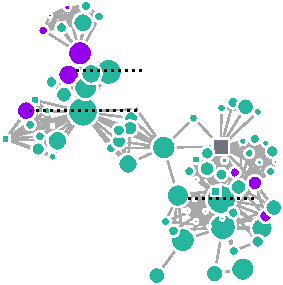
\includegraphics{tidy_stats_files/figure-latex/unnamed-chunk-120-1.pdf}

Пакет \texttt{remotes} можно так же использовать для загрузки пакетов из
Bioconductor:

\begin{Shaded}
\begin{Highlighting}[]
\NormalTok{remotes}\OperatorTok{::}\KeywordTok{install_bioc}\NormalTok{(}\StringTok{"flowCore"}\NormalTok{)}
\end{Highlighting}
\end{Shaded}

\section{Где искать нужные пакеты}\label{where_packages}

Мы разобрались с тем, как устанавливать пакеты. А где же их находить?

Это вопрос гораздо более сложный чем может показаться. Например, можно
работать в R и не знать, что существует пакет, который решает нужную для
вас задачу. Или же найти такой пакет и не знать, что есть более
современный пакет, который делает это еще лучше!

Здесь нет каких-то готовых решений. CRAN пытается создавать и
поддерживать тематические списки \emph{(Task View)} пакетов с описанием
задач, которые они решают:

\url{https://cran.r-project.org/web/views/}

Безусловно, если вы глубоко занимаетесь какой-либо темой из списка, то
стоит изучить соотвестствующий \emph{Task View}, но начинать знакомство
с помощью \emph{Task View} достаточно тяжело.

Другой вариант --- просто погуглить, найти релевантные статьи или книги.
Внимательно смотрите на дату публикации: R --- очень быстро
развивающийся язык, поэтому с большой вероятностью то, что было написано
пять лет назад уже потеряло актуальность. Нет, работать это будет, но,
скорее всего, появился более удобный и продвинутый инструмент.

\chapter{Импорт и экспорт данных}\label{real_data}

Итак, пришло время перейти к реальным данным. Мы начнем с использования
датасета (так мы будем называть любой набор данных) по супергероям. Этот
датасет представляет собой табличку, каждая строка которой - отдельный
супергерой, а столбик --- какая-либо информация о нем. Например, цвет
глаз, цвет волос, вселенная супергероя\footnote{супергерои в комиксах,
  фильмах и телесериалах часто взаимодействуют друг с другом, однако
  обычно это взаимодействие происходит между супергероями одного
  издателя. Два крупнейших издателя комиксов --- DC и Marvel, поэтому
  принято говорить о вселенной DC и Marvel.}, рост, вес, пол и так
далее. Несложно заметить, что этот датасет идеально подходит под
структуру датафрейма: прямоугольная табличка, внутри которой есть разные
колонки, каждая из которой имеет свой тип (числовой или строковый).

\section{Рабочая папка и проекты RStudio}\label{wd}

Для начала скачайте файл по
\href{https://raw.githubusercontent.com/agricolamz/2020-2021-ds4dh/master/data/heroes_information.csv}{ссылке}

Он, скорее всего, появился у Вас в папке ``Загрузки''. Если мы будем
просто пытаться прочитать этот файл (например, с помощью
\texttt{read.csv()} --- мы к этой функцией очень скоро перейдем), указав
его имя и разрешение, то наткнемся на такую ошибку:

\begin{Shaded}
\begin{Highlighting}[]
\KeywordTok{read.csv}\NormalTok{(}\StringTok{"heroes_information.csv"}\NormalTok{)}
\end{Highlighting}
\end{Shaded}

\begin{verbatim}
## Warning in file(file, "rt"): не могу открыть файл 'heroes_information.csv': No
## such file or directory
\end{verbatim}

\begin{verbatim}
## Error in file(file, "rt"): не могу открыть соединение
\end{verbatim}

Это означает, что R не может найти нужный файл. Вообще-то мы даже не
сказали, где искать. Нам нужно как-то совместить место, где R ищет
загружаемые файлы и сами файлы. Для этого есть несколько способов.

\begin{itemize}
\tightlist
\item
  Магомет идет к горе: перемещение файлов в рабочую папку.
\end{itemize}

Для этого нужно узнать, какая папка является рабочей с помощью функции
\texttt{getwd()} (без аргументов), найти эту папку в проводнике и
переместить туда файл. После этого можно использовать просто название
файла с разрешением:

\begin{Shaded}
\begin{Highlighting}[]
\NormalTok{heroes <-}\StringTok{ }\KeywordTok{read.csv}\NormalTok{(}\StringTok{"heroes_information.csv"}\NormalTok{)}
\end{Highlighting}
\end{Shaded}

Кроме того, путь к рабочей папке можно увидеть в RStudio во вкладке с
консолью, в самой верхней части (прямо под надписью ``Console''):

\begin{figure}
\centering

\includegraphics[width=4.16667in]{images/Console_wd.png}
\caption{}
\end{figure}

\begin{itemize}
\tightlist
\item
  Гора идет к Магомету: изменение рабочей папки.
\end{itemize}

Можно просто сменить рабочую папку с помощью \texttt{setwd()} на ту, где
сейчас лежит файл, прописав путь до этой папки. Теперь файл находится в
рабочей папке:

\begin{Shaded}
\begin{Highlighting}[]
\NormalTok{heroes <-}\StringTok{ }\KeywordTok{read.csv}\NormalTok{(}\StringTok{"heroes_information.csv"}\NormalTok{)}
\end{Highlighting}
\end{Shaded}

Этот вариант использовать не рекомендуется! Как минимум, это сразу
делает невозможным запустить скрипт на другом компьютере.

\begin{itemize}
\tightlist
\item
  Гора находит Магомета по месту прописки: указание полного пути файла.
\end{itemize}

\begin{Shaded}
\begin{Highlighting}[]
\NormalTok{heroes <-}\StringTok{ }\KeywordTok{read.csv}\NormalTok{(}\StringTok{"/Users/Username/Some_Folder/heroes_information.csv"}\NormalTok{)}
\end{Highlighting}
\end{Shaded}

Этот вариант страдает теми же проблемами, что и предыдущий, поэтому тоже
не рекомендуется!

\begin{quote}
Для пользователей Windows есть дополнительная сложность: знак \texttt{/}
является особым знаком для R, поэтому вместо него нужно использовать
двойной \texttt{//}.
\end{quote}

\begin{itemize}
\tightlist
\item
  Магомет использует кнопочный интерфейс: Import Dataset.
\end{itemize}

Во вкладке Environment справа в окне RStudio есть кнопка ``Import
Dataset''. Возможно, у Вас возникло непреодолимое желание отдохнуть от
написания кода и понажимать кнопочки --- сопротивляйтесь этому всеми
силами, но не вините себя, если не сдержитесь.

\begin{itemize}
\tightlist
\item
  Гора находит Магомета в интернете.
\end{itemize}

Многие функции в R, предназначенные для чтения файлов, могут прочитать
файл не только на Вашем компьютере, но и сразу из интернета. Для этого
просто используйте ссылку вместо пути:

\begin{Shaded}
\begin{Highlighting}[]
\NormalTok{heroes <-}\StringTok{ }\KeywordTok{read.csv}\NormalTok{(}\StringTok{"https://raw.githubusercontent.com/agricolamz/2020-2021-ds4dh/master/data/heroes_information.csv"}\NormalTok{)}
\end{Highlighting}
\end{Shaded}

\begin{itemize}
\tightlist
\item
  Каждый Магомет получает по своей горе: использование проектов в
  RStudio.
\end{itemize}

На первый взгляд это кажется чем-то очень сложным, но это не так. Это
очень просто и ОЧЕНЬ удобно. При создании проекта создается отдельная
папочка, где у Вас лежат данные, хранятся скрипты, вспомогательные файлы
и отчеты. Если нужно вернуться к другому проекту --- просто открываете
другой проект, с другими файлами и скриптами. Это еще помогает не
пересекаться переменным из разных проектов --- а то, знаете,
использование двух переменных \texttt{data} в разных скриптах чревато
ошибками. Поэтому очень удобным решением будет выделение отдельного
проекта под этот курс.

\begin{quote}
При закрытии проекта все переменные по умолчанию тоже будут сохраняться,
а при открытии --- восстанавливаться. Это очень удобно, хотя некоторые
\href{https://r4ds.had.co.nz/workflow-projects.html}{рекомендуют от
этого отказаться}. Это можно сделать во вкладке
\texttt{Tool\ -\ Global\ Options...}
\end{quote}

\subsection{Табличные данные: текстовые и бинарные
данные}\label{text_binary}

Как Вы уже поняли, импортирование данных - одна из самых муторных и
неприятных вещей в R. Если у Вас получится с этим справится, то все
остальное - ерунда. Мы уже разобрались с первой частью этого процесса -
нахождением файла с данными, осталось научиться их читать.

Здесь стоит сделать небольшую ремарку. Довольно часто данные
представляют собой табличку. Или же их можно свести к табличке. Такая
табличка, как мы уже выяснили, удобно репрезентируется в виде
датафрейма. Но как эти данные хранятся на компьютере? Есть два варианта:
в \emph{бинарном} и в \emph{текстовом} файле.

Текстовый файл означает, что такой файл можно открыть в программе
``Блокнот'' или аналоге (например, TextEdit на macOS) и увидеть
напечатанный текст: скрипт, роман или упорядоченный набор цифр и букв.
Нас сейчас интересует именно последний случай. Таблица может быть
представлена как текст: отдельные строчки в файле будут разделять разные
строчки таблицы, а какой-нибудь знак-разделитель отделять колонки друг
от друга.

Для чтения данных из текстового файла есть довольно удобная функция
\texttt{read.table()}. Почитайте хэлп по ней и ужаснитесь: столько
разных параметров на входе! Но там же вы увидете функции
\texttt{read.csv()}, \texttt{read.csv2()} и некоторые другие --- по
сути, это тот же \texttt{read.table()}, но с другими параметрами по
умолчанию, соответствующие формату файла, который мы загружаем. В данном
случае используется формат .csv, что означает ``Comma Separated Values''
(Значения, Разделенные Запятыми). Формат .csv --- это самый известный
способ хранения табличных данных в файде на сегодняшний день. Файлы с
расширением .csv можно легко открыть в любой программе, работающей с
таблицами, в том числе Microsoft Excel и его аналогах.

Файл с расширением .csv --- это просто текстовый файл, в котором
``закодирована'' таблица: разные строчки разделяют разные строчки
таблицы, а столбцы отделяются запятыми (отсюда и название). Вы можете
вручную создать такие файлы в Блокноте и сохранять их с форматом .csv -
и такая табличка будет нормально открываться в Microsoft Excel и других
программах для работы с таблицами. Можете попробовать это сделать
самостоятельно!

Как говорилось ранее, в качестве разделителя ячеек по горизонтали --- то
есть разделителя между столбцами --- используется запятая. С этим
связана одна проблема: в некоторых странах (в т.ч. и России) принято
использовать запятую для разделения дробной части числа, а не точку, как
это делается в большинстве стран мира. Поэтому есть альтернативный
вариант формата .csv, где значения разделены точкой с запятой
(\texttt{;}), а дробные значения - запятой (\texttt{,}). В этом и
различие функций \texttt{read.csv()} и \texttt{read.csv2()} --- первая
функция предназначена для ``международного'' формата, вторая - для
(условно) ``Российского''. Оба варианта формата имеют расширение .csv,
поэтому заранее понять какой именно будет вариант довольно сложно,
приходится либо пробовать оба, либо заранее открывать файл в текстовом
редакторе.

В первой строчке обычно содержатся названия столбцов - и это чертовски
удобно, функции \texttt{read.csv()} и \texttt{read.csv2()} по умолчанию
считают первую строчку именно как название для колонок.

Кроме .csv формата есть и другие варианты хранения таблиц в виде текста.
Например, .tsv --- тоже самое, что и .csv, но разделитель - знак
табуляции. Для чтения таких файлов есть функция \texttt{read.delim()} и
\texttt{read.delim2()}. Впрочем, даже если бы ее и не было, можно было
бы просто подобрать нужные параметры для функции \texttt{read.table()}.
Есть даже функции, которые пытаются сами ``угадать'' нужные параметры
для чтения --- часто они справляются с этим довольно удачно. Но не
всегда. Поэтому стоит научиться справляться с любого рода данными на
входе.

Итак, прочитаем наш файл. Для этого используем только параметр
\texttt{file\ =}, который идет первым, и для параметра
\texttt{stringsAsFactors\ =} поставим значение \texttt{FALSE}:

\begin{Shaded}
\begin{Highlighting}[]
\NormalTok{heroes <-}\StringTok{ }\KeywordTok{read.csv}\NormalTok{(}\StringTok{"data/heroes_information.csv"}\NormalTok{, }\DataTypeTok{stringsAsFactors =} \OtherTok{FALSE}\NormalTok{)}
\end{Highlighting}
\end{Shaded}

\begin{quote}
Параметр \texttt{stringsAsFactors\ =} задает то, как будут прочитаны
строковые значения - как уже знакомые нам строки или как факторы. По
сути, факторы - это примерно то же самое, что и character, но
закодированные числами. Когда-то это было придумано для экономии
используемых времени и памяти, сейчас же обычно становится просто лишней
морокой. Но некоторые функции требуют именно character, некоторые
factor, в большинстве случаев это без разницы. Но иногда непонимание
может привести к дурацким ошибкам. В данном случае мы просто пока
обойдемся без факторов. Если у вас версия R выше 4.0, то
\texttt{stringsAsFactors\ =} будет \texttt{FALSE} по умолчанию.
\end{quote}

Можете проверить с помощью \texttt{View(heroes)}: все работает! Если же
вылезает какая-то странная ерунда или же просто ошибка - попробуйте
другие функции (\texttt{read.table()}, \texttt{read.delim()}) и
покопаться с параметрами. Для этого читайте \texttt{Help}.

\section{Проверка импортированных
данных}\label{ux43fux440ux43eux432ux435ux440ux43aux430-ux438ux43cux43fux43eux440ux442ux438ux440ux43eux432ux430ux43dux43dux44bux445-ux434ux430ux43dux43dux44bux445}

При импорте данных обратите внимания на предупреждения (если таковые
появляются), в большинстве случаев они указывают на то, что данные
импортированы некорректно.

Проверим, что все прочиталось нормально с помощью уже известной нам
функции \texttt{str()}:

\begin{Shaded}
\begin{Highlighting}[]
\KeywordTok{str}\NormalTok{(heroes)}
\end{Highlighting}
\end{Shaded}

\begin{verbatim}
## 'data.frame':    734 obs. of  11 variables:
##  $ X         : int  0 1 2 3 4 5 6 7 8 9 ...
##  $ name      : chr  "A-Bomb" "Abe Sapien" "Abin Sur" "Abomination" ...
##  $ Gender    : chr  "Male" "Male" "Male" "Male" ...
##  $ Eye.color : chr  "yellow" "blue" "blue" "green" ...
##  $ Race      : chr  "Human" "Icthyo Sapien" "Ungaran" "Human / Radiation" ...
##  $ Hair.color: chr  "No Hair" "No Hair" "No Hair" "No Hair" ...
##  $ Height    : num  203 191 185 203 -99 193 -99 185 173 178 ...
##  $ Publisher : chr  "Marvel Comics" "Dark Horse Comics" "DC Comics" "Marvel Comics" ...
##  $ Skin.color: chr  "-" "blue" "red" "-" ...
##  $ Alignment : chr  "good" "good" "good" "bad" ...
##  $ Weight    : int  441 65 90 441 -99 122 -99 88 61 81 ...
\end{verbatim}

\begin{quote}
Всегда проверяйте данные на входе и никогда не верьте на слово, если вам
говорят, что данные вычищенные и не содержат никаких ошибок.
\end{quote}

На что нужно обращать внимание?

\begin{enumerate}
\def\labelenumi{\arabic{enumi}.}
\item
  Прочитаны ли пропущенные значения как \texttt{NA}. По умолчанию
  пропущенные значения обозначаются пропущенной строчкой или ``NA'', но
  встречаются самые разнообразные варианты. Возможные варианты
  кодирования пропущенных значений можно задать в параметре
  \texttt{na.strings\ =} функции \texttt{read.table()} и ее вариантов. В
  нашем датасете как раз такая ситуация, где нужно самостоятельно
  задавать, какие значения будут прочитаны как \texttt{NA}. Попытайтесь
  самостоятельно догадаться, как именно.
\item
  Прочитаны ли те столбики, которые должны быть числовыми, как
  \texttt{int} или \texttt{num}. Если в колонке содержатся числа, а
  написано \texttt{chr} (= \texttt{"character"}) или \texttt{Factor} (в
  случае если \texttt{stringsAsFactors\ =\ TRUE}), то, скорее всего,
  одна из строчек содержит в себе нечисловые знаки, которые не были
  прочитаны как \texttt{NA}.
\item
  Странные названия колонок. Это может случиться по самым разным
  причинам, но в таких случаях стоит открывать файл в другой программе и
  смотреть первые строчки. Например, может оказаться, что первые
  несколько строчек --- пустые или что первая строчка не содержит
  название столбцов (тогда для параметра \texttt{header\ =} нужно
  поставить \texttt{FALSE})
\item
  Вместо строковых данных у вас кракозябры. Это означает проблемы с
  кодировкой. В первую очередь попробуйте выставить значение
  \texttt{"UTF-8"} для параметра \texttt{encoding\ =} в функции для
  чтения файла:
\end{enumerate}

\begin{Shaded}
\begin{Highlighting}[]
\NormalTok{heroes <-}\StringTok{ }\KeywordTok{read.csv}\NormalTok{(}\StringTok{"data/heroes_information.csv"}\NormalTok{, }
                   \DataTypeTok{stringsAsFactors =} \OtherTok{FALSE}\NormalTok{,}
                   \DataTypeTok{encoding =} \StringTok{"UTF-8"}\NormalTok{)}
\end{Highlighting}
\end{Shaded}

В случае если это не помогает, попробуйте
\href{https://www.artlebedev.ru/decoder/}{разобрать}, что это за
кодировка.

\begin{enumerate}
\def\labelenumi{\arabic{enumi}.}
\setcounter{enumi}{4}
\item
  Все прочиталось как одна колонка. В этом случае, скорее всего,
  неправильно подобран разделить колонок --- параметр \texttt{sep\ =}.
  Откройте файл в текстовом редакторе, чтобы понять какой нужно
  использовать.
\item
  В отдельных строчках все прочиталось как одна колонка, а в остальных
  нормально. Скорее всего, в файле есть значения типа
  \texttt{\textbackslash{}} или \texttt{"}, которые в функциях
  \texttt{read.csv()}, \texttt{read.delim()}, \texttt{read.csv2()},
  \texttt{read.delim2()} читаются как символы для закавычивания
  значений. Это может понадобиться, если у вас в таблице есть строковые
  значения со знаками \texttt{,} или \texttt{;}, которые могут
  восприниматься как разделитель столбцов.
\item
  Появились какие-то новые числовые колонки. Возможно неправильно
  поставлен разделитель дробной части. Обычно это либо \texttt{.}
  (\texttt{read.table()}, \texttt{read.csv()}, \texttt{read.delim()}),
  либо \texttt{,} (\texttt{read.csv2()}, \texttt{read.delim2()}).
\end{enumerate}

Конкретно в нашем случае все прочиталось хорошо с помощью функции
\texttt{read.csv()}, но в строковых переменных есть много прочерков,
которые обозначают отсутствие информации по данному параметру
супергероя, т.е. пропущенное значение. А вот с числовыми значениями все
не так просто: для всех супергероев прописано какое-то число, но во
многих случаях это -99. Очевидно, отрицательного роста и массы не
бывает, это просто обозначение пропущенных значений (такое часто
используется). Таким образом, чтобы адекватно прочитать файл, нам нужно
поменять параметр \texttt{na.strings\ =} функции \texttt{read.csv()}:

\begin{Shaded}
\begin{Highlighting}[]
\NormalTok{heroes <-}\StringTok{ }\KeywordTok{read.csv}\NormalTok{(}\StringTok{"data/heroes_information.csv"}\NormalTok{, }
                   \DataTypeTok{stringsAsFactors =} \OtherTok{FALSE}\NormalTok{,}
                   \DataTypeTok{na.strings =} \KeywordTok{c}\NormalTok{(}\StringTok{"-"}\NormalTok{, }\StringTok{"-99"}\NormalTok{))}
\end{Highlighting}
\end{Shaded}

\section{Экспорт данных}\label{export_data}

Представим, что вы хотите сохранить табличку с данными про супергероев
из вселенной DC в виде отдельного файла .csv.

\begin{Shaded}
\begin{Highlighting}[]
\NormalTok{dc <-}\StringTok{ }\NormalTok{heroes[heroes}\OperatorTok{$}\NormalTok{Publisher }\OperatorTok{==}\StringTok{ "DC Comics"}\NormalTok{,]}
\end{Highlighting}
\end{Shaded}

Функция \texttt{write.csv()} позволит записать датафрейм в файл формата
.csv:

\begin{Shaded}
\begin{Highlighting}[]
\KeywordTok{write.csv}\NormalTok{(dc, }\StringTok{"data/dc_heroes_information.csv"}\NormalTok{)}
\end{Highlighting}
\end{Shaded}

Обычно названия строк не используются, и их лучше не записывать,
поставив для \texttt{row.names\ =} значение \texttt{FALSE}:

\begin{Shaded}
\begin{Highlighting}[]
\KeywordTok{write.csv}\NormalTok{(dc, }\StringTok{"data/dc_heroes_information.csv"}\NormalTok{, }\DataTypeTok{row.names =} \OtherTok{FALSE}\NormalTok{)}
\end{Highlighting}
\end{Shaded}

По аналогии с \texttt{read.csv2()}, \texttt{write.csv2()} позволит
записать файлы формата .csv с разделителем \texttt{;}.

\begin{Shaded}
\begin{Highlighting}[]
\KeywordTok{write.csv2}\NormalTok{(dc, }\StringTok{"data/dc_heroes_information.csv"}\NormalTok{, }\DataTypeTok{row.names =} \OtherTok{FALSE}\NormalTok{)}
\end{Highlighting}
\end{Shaded}

\section{Импорт таблиц в бинарном формате: таблицы Excel,
SPSS}\label{binary}

Тем не менее, далеко не всегда таблицы представлены в виде текстового
файла. Самый распространенный пример таблицы в бинарном виде --- родные
форматы Microsoft Excel. Если Вы попробуете открыть .xlsx файл в
Блокноте, то увидите кракозябры. Это делает работу с этим файлами
гораздо менее удобной, поэтому стоит избегать экселевских форматов и
стараться все сохранять в .csv.

Такие файлы не получится прочитать при помощи базового инструментария R.
Тем не менее, для чтения таких файлов есть много дополнительных пакетов:

\begin{itemize}
\item
  файлы Microsoft Excel: лучше всего справляется пакет \texttt{readxl}
  (является частью расширенного tidyverse), у него есть много
  альтернатив (\texttt{xlsx}, \texttt{openxlsx}).
\item
  файлы SPSS, SAS, Stata: существуют два основных пакета ---
  \texttt{haven} (часть расширенного tidyverse) и \texttt{foreign}.
\end{itemize}

Что такое пакеты и как их устанавливать мы изучим очень скоро.

\section{Быстрый импорт данных}\label{fastread}

Чтение табличных данных обычно происходит очень быстро. По крайней мере,
до тех пор пока ваши данные не содержат очень много значений. Если вы
попробуете прочитать с помощью \texttt{read.csv()} таблицу с миллионами
строчками, то заметите, что это происходит довольно медленно. Впрочем,
эта проблема эффективно решается дополнительными пакетами.

\begin{itemize}
\tightlist
\item
  Пакет \texttt{readr} (часть базового tidyverse) предлагает функции,
  очень похожие на стандартные \texttt{read.csv()}, \texttt{read.csv2()}
  и тому подобные, только в названиях используется нижнее подчеркивание:
  \texttt{read\_csv()} и \texttt{read\_csv2()}. Они быстрее и немного
  удобнее, особенно если вы работаете в tidyverse.
\end{itemize}

\begin{Shaded}
\begin{Highlighting}[]
\NormalTok{readr}\OperatorTok{::}\KeywordTok{read_csv}\NormalTok{(}\StringTok{"data/heroes_information.csv"}\NormalTok{,}
         \DataTypeTok{na =} \KeywordTok{c}\NormalTok{(}\StringTok{"-"}\NormalTok{, }\StringTok{"-99"}\NormalTok{))}
\end{Highlighting}
\end{Shaded}

\begin{verbatim}
## Warning: Missing column names filled in: 'X1' [1]
\end{verbatim}

\begin{verbatim}
## 
## -- Column specification --------------------------------------------------------
## cols(
##   X1 = col_double(),
##   name = col_character(),
##   Gender = col_character(),
##   `Eye color` = col_character(),
##   Race = col_character(),
##   `Hair color` = col_character(),
##   Height = col_double(),
##   Publisher = col_character(),
##   `Skin color` = col_character(),
##   Alignment = col_character(),
##   Weight = col_double()
## )
\end{verbatim}

\begin{verbatim}
## # A tibble: 734 x 11
##       X1 name  Gender `Eye color` Race  `Hair color` Height Publisher
##    <dbl> <chr> <chr>  <chr>       <chr> <chr>         <dbl> <chr>    
##  1     0 A-Bo~ Male   yellow      Human No Hair         203 Marvel C~
##  2     1 Abe ~ Male   blue        Icth~ No Hair         191 Dark Hor~
##  3     2 Abin~ Male   blue        Unga~ No Hair         185 DC Comics
##  4     3 Abom~ Male   green       Huma~ No Hair         203 Marvel C~
##  5     4 Abra~ Male   blue        Cosm~ Black            NA Marvel C~
##  6     5 Abso~ Male   blue        Human No Hair         193 Marvel C~
##  7     6 Adam~ Male   blue        <NA>  Blond            NA NBC - He~
##  8     7 Adam~ Male   blue        Human Blond           185 DC Comics
##  9     8 Agen~ Female blue        <NA>  Blond           173 Marvel C~
## 10     9 Agen~ Male   brown       Human Brown           178 Marvel C~
## # ... with 724 more rows, and 3 more variables: `Skin color` <chr>,
## #   Alignment <chr>, Weight <dbl>
\end{verbatim}

\begin{itemize}
\tightlist
\item
  Пакет \texttt{vroom} - это часть расширенного tidyverse. Это такая
  альтернатива \texttt{readr} из того же tidyverse, но еще быстрее
  (отсюда и название).
\end{itemize}

\begin{Shaded}
\begin{Highlighting}[]
\NormalTok{vroom}\OperatorTok{::}\KeywordTok{vroom}\NormalTok{(}\StringTok{"data/heroes_information.csv"}\NormalTok{)}
\end{Highlighting}
\end{Shaded}

\begin{verbatim}
## New names:
## * `` -> ...1
\end{verbatim}

\begin{verbatim}
## Rows: 734
## Columns: 11
## Delimiter: ","
## chr [8]: name, Gender, Eye color, Race, Hair color, Publisher, Skin color, Alignment
## dbl [3]: ...1, Height, Weight
## 
## Use `spec()` to retrieve the guessed column specification
## Pass a specification to the `col_types` argument to quiet this message
\end{verbatim}

\begin{verbatim}
## # A tibble: 734 x 11
##     ...1 name  Gender `Eye color` Race  `Hair color` Height Publisher
##    <dbl> <chr> <chr>  <chr>       <chr> <chr>         <dbl> <chr>    
##  1     0 A-Bo~ Male   yellow      Human No Hair         203 Marvel C~
##  2     1 Abe ~ Male   blue        Icth~ No Hair         191 Dark Hor~
##  3     2 Abin~ Male   blue        Unga~ No Hair         185 DC Comics
##  4     3 Abom~ Male   green       Huma~ No Hair         203 Marvel C~
##  5     4 Abra~ Male   blue        Cosm~ Black           -99 Marvel C~
##  6     5 Abso~ Male   blue        Human No Hair         193 Marvel C~
##  7     6 Adam~ Male   blue        -     Blond           -99 NBC - He~
##  8     7 Adam~ Male   blue        Human Blond           185 DC Comics
##  9     8 Agen~ Female blue        -     Blond           173 Marvel C~
## 10     9 Agen~ Male   brown       Human Brown           178 Marvel C~
## # ... with 724 more rows, and 3 more variables: `Skin color` <chr>,
## #   Alignment <chr>, Weight <dbl>
\end{verbatim}

\begin{itemize}
\tightlist
\item
  Пакет \texttt{data.table} - это не просто пакет, а целый фреймворк для
  работы с R, основной конкурент tidyverse. Одна из основных фишек
  \texttt{data.table} - быстрота работы. Это касается не только
  процессинга данных, но и их загрузки и записи. Поэтому некоторые
  используют функции \texttt{data.table} для чтения и записи данных в
  отдельности от всего остального пакета - они даже и называются
  соответствующе: \texttt{fread()} и \texttt{fwrite()}, где \textbf{f}
  означет \textbf{f}ast\footnote{А еще \textbf{f}riendly:
    \texttt{fread()} обычно самостоятельно хорошо угадывает формат
    таблицы на входе. \texttt{vroom} тоже так умеет.}.
\end{itemize}

\begin{Shaded}
\begin{Highlighting}[]
\NormalTok{data.table}\OperatorTok{::}\KeywordTok{fread}\NormalTok{(}\StringTok{"data/heroes_information.csv"}\NormalTok{)}
\end{Highlighting}
\end{Shaded}

\begin{verbatim}
##       V1            name Gender Eye color              Race       Hair color
##   1:   0          A-Bomb   Male    yellow             Human          No Hair
##   2:   1      Abe Sapien   Male      blue     Icthyo Sapien          No Hair
##   3:   2        Abin Sur   Male      blue           Ungaran          No Hair
##   4:   3     Abomination   Male     green Human / Radiation          No Hair
##   5:   4         Abraxas   Male      blue     Cosmic Entity            Black
##  ---                                                                        
## 730: 729 Yellowjacket II Female      blue             Human Strawberry Blond
## 731: 730            Ymir   Male     white       Frost Giant          No Hair
## 732: 731            Yoda   Male     brown    Yoda's species            White
## 733: 732         Zatanna Female      blue             Human            Black
## 734: 733            Zoom   Male       red                 -            Brown
##      Height         Publisher Skin color Alignment Weight
##   1:  203.0     Marvel Comics          -      good    441
##   2:  191.0 Dark Horse Comics       blue      good     65
##   3:  185.0         DC Comics        red      good     90
##   4:  203.0     Marvel Comics          -       bad    441
##   5:  -99.0     Marvel Comics          -       bad    -99
##  ---                                                     
## 730:  165.0     Marvel Comics          -      good     52
## 731:  304.8     Marvel Comics      white      good    -99
## 732:   66.0      George Lucas      green      good     17
## 733:  170.0         DC Comics          -      good     57
## 734:  185.0         DC Comics          -       bad     81
\end{verbatim}

Чем же пользоваться среди всего этого многообразия?
\href{https://www.danielecook.com/speeding-up-reading-and-writing-in-r/}{Бенчмарки}\footnote{бенчмаркинг
  --- это тест производительности, в данном случае --- сравнение
  скорости работы конкурирующих пакетов.} показывают, что быстрее всех
\texttt{vroom} и \texttt{data.table}. Если же у вас нет задачи ускорить
работу кода на несколько миллисекунд или прочитать датасет на много
миллионов строк, то стандартного \texttt{read.csv()} (если вы работаете
в базовом R) и \texttt{readr::read\_csv()} (если вы работаете в
tidyverse) должно быть достаточно.

Все перечисленные пакеты повзоляют не только быстро импортировать
данные, но и быстро (и удобно!) экспортировать их:

\begin{Shaded}
\begin{Highlighting}[]
\NormalTok{readr}\OperatorTok{::}\KeywordTok{write_csv}\NormalTok{(dc, }\StringTok{"data/dc_heroes_information.csv"}\NormalTok{)}
\NormalTok{readr}\OperatorTok{::}\KeywordTok{write_excel_csv}\NormalTok{(dc, }\StringTok{"data/dc_heroes_information.csv"}\NormalTok{) }\CommentTok{#Если в Excel возникают проблемы с кодировками при открытии созданного .csv файла, то эта функция решает эти проблемы}
\NormalTok{vroom}\OperatorTok{::}\KeywordTok{vroom_write}\NormalTok{(dc, }\StringTok{"data/dc_heroes_information.csv"}\NormalTok{, }\DataTypeTok{delim =} \StringTok{","}\NormalTok{)}
\NormalTok{data.table}\OperatorTok{::}\KeywordTok{fwrite}\NormalTok{(dc, }\StringTok{"data/dc_heroes_information.csv"}\NormalTok{)}
\end{Highlighting}
\end{Shaded}

В плане скорости записи файлов соотношение сил примерно такое же, как и
для чтения: \texttt{vroom} и \texttt{data.table} обгоняют всех, затем
идет \texttt{readr}, и только после него - базовые функции R.

\chapter{Условные конструкции и циклы}\label{loops_conditions}

\section{\texorpdfstring{Выражения \texttt{if}, \texttt{else},
\texttt{else\ if}}{Выражения if, else, else if}}\label{if}

Стандратная часть практически любого языка программирования --- условные
конструкции. R не исключение. Однако и здесь есть свои особенности.
Начнем с самого простого варианта с одним условием. Выглядеть условная
конcтрукция будет вот так:

\begin{verbatim}
if (условие) выражение
\end{verbatim}

Вот так это будет работать на практике:

\begin{Shaded}
\begin{Highlighting}[]
\NormalTok{number <-}\StringTok{ }\DecValTok{1}
\ControlFlowTok{if}\NormalTok{ (number }\OperatorTok{>}\StringTok{ }\DecValTok{0}\NormalTok{) }\StringTok{"Положительное число"}
\end{Highlighting}
\end{Shaded}

\begin{verbatim}
## [1] "Положительное число"
\end{verbatim}

Если выражение (expression) содержит больше одной строчки, то они
объединяются фигурными скобками. Впрочем, использовать их можно, даже
если строчка всего в выражении всего одна.

\begin{Shaded}
\begin{Highlighting}[]
\NormalTok{number <-}\StringTok{ }\DecValTok{1}
\ControlFlowTok{if}\NormalTok{ (number }\OperatorTok{>}\StringTok{ }\DecValTok{0}\NormalTok{) \{}
  \StringTok{"Положительное число"}
\NormalTok{\}}
\end{Highlighting}
\end{Shaded}

\begin{verbatim}
## [1] "Положительное число"
\end{verbatim}

В рассмотренной нами конструкции происходит проверка на условие. Если
условие верно\footnote{В принципе, необязательно внутри должна быть
  проверка условий, достаточно просто значения \texttt{TRUE}.}, то
происходит то, что записано в последующем выражении. Если же условие
неверно\footnote{Аналогично, достаточно просто значения \texttt{FALSE}.},
то ничего не происходит.

Оператор \texttt{else} позволяет задавать действие на все остальные
случаи:

\begin{verbatim}
if (условие) выражение else выражение
\end{verbatim}

Работает это так:

\begin{Shaded}
\begin{Highlighting}[]
\NormalTok{number <-}\StringTok{ }\OperatorTok{-}\DecValTok{3}
\ControlFlowTok{if}\NormalTok{ (number }\OperatorTok{>}\StringTok{ }\DecValTok{0}\NormalTok{) \{}
  \StringTok{"Положительное число"}
\NormalTok{\} }\ControlFlowTok{else}\NormalTok{ \{}
  \StringTok{"Отрицательное число или ноль"}
\NormalTok{\}}
\end{Highlighting}
\end{Shaded}

\begin{verbatim}
## [1] "Отрицательное число или ноль"
\end{verbatim}

Иногда нам нужна последовательная проверка на несколько условий. Для
этого есть оператор \texttt{else\ if}. Вот как выглядит ее применение:

\begin{Shaded}
\begin{Highlighting}[]
\NormalTok{number <-}\StringTok{ }\DecValTok{0}
\ControlFlowTok{if}\NormalTok{ (number }\OperatorTok{>}\StringTok{ }\DecValTok{0}\NormalTok{) \{}
  \StringTok{"Положительное число"}
\NormalTok{\} }\ControlFlowTok{else} \ControlFlowTok{if}\NormalTok{ (number }\OperatorTok{<}\StringTok{ }\DecValTok{0}\NormalTok{)\{}
  \StringTok{"Отрицательное число"}
\NormalTok{\} }\ControlFlowTok{else}\NormalTok{ \{}
  \StringTok{"Ноль"}
\NormalTok{\}}
\end{Highlighting}
\end{Shaded}

\begin{verbatim}
## [1] "Ноль"
\end{verbatim}

Как мы помним, R --- язык, в котором векторизация играет большое
значение. Но вот незадача --- условные конструкции не векторизованы в R!
Давайте попробуем применить эти конструкции для вектора значений и
посмотрим, что получится.

\begin{Shaded}
\begin{Highlighting}[]
\NormalTok{number <-}\StringTok{ }\OperatorTok{-}\DecValTok{2}\OperatorTok{:}\DecValTok{2}
\ControlFlowTok{if}\NormalTok{ (number }\OperatorTok{>}\StringTok{ }\DecValTok{0}\NormalTok{) \{}
  \StringTok{"Положительное число"}
\NormalTok{\} }\ControlFlowTok{else} \ControlFlowTok{if}\NormalTok{ (number }\OperatorTok{<}\StringTok{ }\DecValTok{0}\NormalTok{)\{}
  \StringTok{"Отрицательное число"}
\NormalTok{\} }\ControlFlowTok{else}\NormalTok{ \{}
  \StringTok{"Ноль"}
\NormalTok{\}}
\end{Highlighting}
\end{Shaded}

\begin{verbatim}
## Warning in if (number > 0) {: длина условия > 1, будет использован только первый
## элемент
\end{verbatim}

\begin{verbatim}
## Warning in if (number < 0) {: длина условия > 1, будет использован только первый
## элемент
\end{verbatim}

\begin{verbatim}
## [1] "Отрицательное число"
\end{verbatim}

R выдает сообщение, что используется только первое значение логического
вектора внутри условия. Остальные просто игнорируются. Как же посчитать
для всего вектора сразу?

\section{\texorpdfstring{Циклы \texttt{for}}{Циклы for}}\label{for}

Во-первых, можно использовать \texttt{for}. Синтаксис у \texttt{for}
похож на синтаксис условных конструкций.

\begin{verbatim}
for(переменная in последовательность) выражение
\end{verbatim}

Теперь мы можем объединить условные конструкции и \texttt{for}. Немножко
монструозно, но это работает:

\begin{Shaded}
\begin{Highlighting}[]
\ControlFlowTok{for}\NormalTok{ (i }\ControlFlowTok{in}\NormalTok{ number) \{}
  \ControlFlowTok{if}\NormalTok{ (i }\OperatorTok{>}\StringTok{ }\DecValTok{0}\NormalTok{) \{}
    \KeywordTok{print}\NormalTok{(}\StringTok{"Положительное число"}\NormalTok{)}
\NormalTok{  \} }\ControlFlowTok{else} \ControlFlowTok{if}\NormalTok{ (i }\OperatorTok{<}\StringTok{ }\DecValTok{0}\NormalTok{) \{}
    \KeywordTok{print}\NormalTok{(}\StringTok{"Отрицательное число"}\NormalTok{)}
\NormalTok{  \} }\ControlFlowTok{else}\NormalTok{ \{}
    \KeywordTok{print}\NormalTok{(}\StringTok{"Ноль"}\NormalTok{)}
\NormalTok{  \}}
\NormalTok{\}}
\end{Highlighting}
\end{Shaded}

\begin{verbatim}
## [1] "Отрицательное число"
## [1] "Отрицательное число"
## [1] "Ноль"
## [1] "Положительное число"
## [1] "Положительное число"
\end{verbatim}

\begin{quote}
Чтобы выводить в консоль результат вычислений внутри \texttt{for}, нужно
использовать \texttt{print()}.
\end{quote}

Здесь стоит отметить, что \texttt{for} используется в R относительно
редко. В подавляющем числе ситуаций использование \texttt{for} можно
избежать. Обычно мы работаем в R с векторами или датафреймами, которые
представляют собой множество относительно независимых наблюдений. Если
мы хотим провести какие-нибудь операции с этими наблюдениями, то они
обычно могут быть выполнены параллельно. Скажем, вы хотите для каждого
испытуемого пересчитать его массу из фунтов в килограммы. Этот пересчет
осуществляется по одинаковой формуле для каждого испытуемого. Эта
формула не изменится из-за того, что какой-то испытуемый слишком большой
или слишком маленький - для следующего испытуемого формула будет
прежняя. Если Вы встречаете подобную задачу (где функцию можно применить
независимо для всех значений), то без цикла \texttt{for} вполне можно
обойтись.

Даже во многих случаях, где расчеты для одной строчки зависят от
расчетов предыдущих строчек, можно обойтись без \texttt{for}
векторизованными функциями, например, \texttt{cumsum()} для подсчета
кумулятивной суммы.

\begin{Shaded}
\begin{Highlighting}[]
\KeywordTok{cumsum}\NormalTok{(}\DecValTok{1}\OperatorTok{:}\DecValTok{10}\NormalTok{)}
\end{Highlighting}
\end{Shaded}

\begin{verbatim}
##  [1]  1  3  6 10 15 21 28 36 45 55
\end{verbatim}

Если же нет подходящей векторизованной функции, то можно воспользоваться
семейством функций \texttt{apply()} (см. @ref(apply\_f) ).

\begin{quote}
После этих объяснений кому-то может показаться странным, что я вообще
упоминаю про эти циклы. Но для кого-то циклы \texttt{for} настолько
привычны, что их полное отсутствие в курсе может показаться еще более
странным. Поэтому лучше от меня, чем на улице.
\end{quote}

Зачем вообще избегать конструкций \texttt{for}? Некоторые говорят, что
они слишком медленные, и частично это верно, если мы сравниваем с
векторизованными функциями, которые написаны на более низкоуровневых
языках. Но в большинстве случаев низкая скорость \texttt{for} связана с
неправильным использованием этой конструкции. Например, стоит избегать
ситуации, когда на каждой итерации \texttt{for} какой-то объект (вектор,
список, что угодно) изменяется в размере. Лучше будет создать заранее
объект нужного размера, который затем будет наполняться значениями:

\begin{Shaded}
\begin{Highlighting}[]
\NormalTok{number_descriptions <-}\StringTok{ }\KeywordTok{character}\NormalTok{(}\KeywordTok{length}\NormalTok{(number)) }\CommentTok{#создаем строковый вектор с такой же длиной, как и исходный вектор}
\ControlFlowTok{for}\NormalTok{ (i }\ControlFlowTok{in} \DecValTok{1}\OperatorTok{:}\KeywordTok{length}\NormalTok{(number)) \{}
  \ControlFlowTok{if}\NormalTok{ (number[i] }\OperatorTok{>}\StringTok{ }\DecValTok{0}\NormalTok{) \{}
\NormalTok{    number_descriptions[i] <-}\StringTok{ "Положительное число"}
\NormalTok{  \} }\ControlFlowTok{else} \ControlFlowTok{if}\NormalTok{ (number[i] }\OperatorTok{<}\StringTok{ }\DecValTok{0}\NormalTok{) \{}
\NormalTok{    number_descriptions[i] <-}\StringTok{ "Отрицательное число"}
\NormalTok{  \} }\ControlFlowTok{else}\NormalTok{ \{}
\NormalTok{    number_descriptions[i] <-}\StringTok{ "Ноль"}
\NormalTok{  \}}
\NormalTok{\}}
\NormalTok{number_descriptions}
\end{Highlighting}
\end{Shaded}

\begin{verbatim}
## [1] "Отрицательное число" "Отрицательное число" "Ноль"               
## [4] "Положительное число" "Положительное число"
\end{verbatim}

В общем, при правильном обращении с \texttt{for} особых проблем со
скоростью не будет. Но все равно это будет громоздкая конструкция, в
которой легко ошибиться, и которую, скорее всего, можно заменить одной
короткой строчкой. Кроме того, без конструкции \texttt{for} код обычно
легко превратить в набор функций, последовательно применяющихся к
данным, что мы будем по максимуму использовать, работая в tidyverse и
применяя пайпы (см. {[}pipe{]}).

\section{\texorpdfstring{Векторизованные условные конструкции: функции
\texttt{ifelse()} и
\texttt{dplyr::case\_when()}}{Векторизованные условные конструкции: функции ifelse() и dplyr::case\_when()}}\label{ifelse}

Альтернатива сочетанию условных конструкций и циклов \texttt{for}
является использование встроенной функции \texttt{ifelse()}. Функция
\texttt{ifelse()} принимает три аргумента - 1) условие (т.е. просто
логический вектор, состоящий из \texttt{TRUE} и \texttt{FALSE}), 2) что
выдавать в случае \texttt{TRUE}, 3) что выдавать в случае
\texttt{FALSE}. На выходе получается вектор такой же длины, как и
изначальный логический вектор (условие).

\begin{Shaded}
\begin{Highlighting}[]
\KeywordTok{ifelse}\NormalTok{(number }\OperatorTok{>}\StringTok{ }\DecValTok{0}\NormalTok{, }\StringTok{"Положительное число"}\NormalTok{, }\StringTok{"Отрицательное число или ноль"}\NormalTok{)}
\end{Highlighting}
\end{Shaded}

\begin{verbatim}
## [1] "Отрицательное число или ноль" "Отрицательное число или ноль"
## [3] "Отрицательное число или ноль" "Положительное число"         
## [5] "Положительное число"
\end{verbatim}

\begin{quote}
Периодически я встречаю у студентов строчку вроде такой:
\texttt{ifelse(условие,\ TRUE,\ FALSE)}. Эта конструкция избыточна, т.к.
получается, что логический вектор из \texttt{TRUE} и \texttt{FALSE}
превращается в абсолютно такой же вектор из \texttt{TRUE} и
\texttt{FALSE} на тех же самых местах. Выходит, что ничего не меняется!
\end{quote}

У \texttt{ifelse()} тоже есть недостаток: он не может включать в себя
дополнительных условий по типу \texttt{else\ if}. В простых ситуациях
можно вставлять \texttt{ifelse()} внутри \texttt{ifelse()}:

\begin{Shaded}
\begin{Highlighting}[]
\KeywordTok{ifelse}\NormalTok{(number }\OperatorTok{>}\StringTok{ }\DecValTok{0}\NormalTok{,}
       \StringTok{"Положительное число"}\NormalTok{,}
       \KeywordTok{ifelse}\NormalTok{(number }\OperatorTok{<}\StringTok{ }\DecValTok{0}\NormalTok{, }\StringTok{"Отрицательное число"}\NormalTok{, }\StringTok{"Ноль"}\NormalTok{))}
\end{Highlighting}
\end{Shaded}

\begin{verbatim}
## [1] "Отрицательное число" "Отрицательное число" "Ноль"               
## [4] "Положительное число" "Положительное число"
\end{verbatim}

Достаточно симпатичное решение предлогает пакет \texttt{dplyr} (основа
tidyverse) --- функция \texttt{case\_when()}, которая работает с
использованием формулы:

\begin{Shaded}
\begin{Highlighting}[]
\NormalTok{dplyr}\OperatorTok{::}\KeywordTok{case_when}\NormalTok{(}
\NormalTok{  number }\OperatorTok{>}\StringTok{ }\DecValTok{0} \OperatorTok{~}\StringTok{ "Положительное число"}\NormalTok{,}
\NormalTok{  number }\OperatorTok{<}\StringTok{ }\DecValTok{0} \OperatorTok{~}\StringTok{ "Отрицательное число"}\NormalTok{,}
\NormalTok{  number }\OperatorTok{==}\StringTok{ }\DecValTok{0} \OperatorTok{~}\StringTok{ "Ноль"}\NormalTok{)}
\end{Highlighting}
\end{Shaded}

\begin{verbatim}
## [1] "Отрицательное число" "Отрицательное число" "Ноль"               
## [4] "Положительное число" "Положительное число"
\end{verbatim}

\chapter{Функциональное программирование в R}\label{functional}

\section{Создание функций}\label{create_fun}

Поздравляю, сейчас мы выйдем на качественно новый уровень владения R.
Вместо того, чтобы пользоваться теми функциями, которые уже написали за
нас, мы можем сами создавать свои функции! В этом нет ничего сложного.

Синтаксис создания функции внешне похож на создание циклов или условных
конструкций. Мы пишем ключевое слово \texttt{function}, в круглых
скобках обозначаем переменные, с которыми собираемся что-то делать.
Внутри фигурных скобок пишем выражения, которые будут выполняться при
запуске функции. У функции есть свое собственное окружение --- место,
где хранятся переменные. Именно те объекты, которые мы передаем в
скобочках, и будут в окружении, так же как и ``обычные'' переменные для
нас в глобальном окружении. Это означает, что функция будет искать
переменные в первую очередь среди объектов, которые переданы в круглых
скобочках. С ними функция и будет работать. На выходе функция выдаст то,
что вычисляется внутри функции \texttt{return()}. Если \texttt{return()}
появляется в теле функции несколько раз, то до результат будет
возвращаться из той функции \texttt{return()}, до которой выполнение
дошло первым.

\begin{Shaded}
\begin{Highlighting}[]
\NormalTok{pow <-}\StringTok{ }\ControlFlowTok{function}\NormalTok{(x, p) \{}
\NormalTok{  power <-}\StringTok{ }\NormalTok{x }\OperatorTok{^}\StringTok{ }\NormalTok{p}
  \KeywordTok{return}\NormalTok{(power)}
\NormalTok{\}}
\KeywordTok{pow}\NormalTok{(}\DecValTok{3}\NormalTok{, }\DecValTok{2}\NormalTok{)}
\end{Highlighting}
\end{Shaded}

\begin{verbatim}
## [1] 9
\end{verbatim}

Если функция проработала до конца, а функция \texttt{return()} так и не
встретилась, то возвращается последнее посчитанное значение.

\begin{Shaded}
\begin{Highlighting}[]
\NormalTok{pow <-}\StringTok{ }\ControlFlowTok{function}\NormalTok{(x, p) \{}
\NormalTok{  x }\OperatorTok{^}\StringTok{ }\NormalTok{p}
\NormalTok{\}}
\KeywordTok{pow}\NormalTok{(}\DecValTok{3}\NormalTok{, }\DecValTok{2}\NormalTok{)}
\end{Highlighting}
\end{Shaded}

\begin{verbatim}
## [1] 9
\end{verbatim}

Если в последней строчке будет присвоение, то функция ничего не вернет
обратно. Это очень распространенная ошибка: функция вроде бы работает
правильно, но ничего не возвращает. Нужно писать так, как будто бы в
последней строчке результат выполнения выводится в консоль.

\begin{Shaded}
\begin{Highlighting}[]
\NormalTok{pow <-}\StringTok{ }\ControlFlowTok{function}\NormalTok{(x, p) \{}
\NormalTok{  power <-}\StringTok{ }\NormalTok{x }\OperatorTok{^}\StringTok{ }\NormalTok{p }\CommentTok{#Функция ничего не вернет, потому что в последней строчке присвоение!}
\NormalTok{\}}
\KeywordTok{pow}\NormalTok{(}\DecValTok{3}\NormalTok{, }\DecValTok{2}\NormalTok{) }\CommentTok{#ничего не возвращается из функции}
\end{Highlighting}
\end{Shaded}

Если функция небольшая, то ее можно записать в одну строчку без фигурных
скобок.

\begin{Shaded}
\begin{Highlighting}[]
\NormalTok{pow <-}\StringTok{ }\ControlFlowTok{function}\NormalTok{(x, p) x }\OperatorTok{^}\StringTok{ }\NormalTok{p}
\KeywordTok{pow}\NormalTok{(}\DecValTok{3}\NormalTok{, }\DecValTok{2}\NormalTok{) }
\end{Highlighting}
\end{Shaded}

\begin{verbatim}
## [1] 9
\end{verbatim}

Вообще, фигурные скобки используются для того, чтобы выполнить серию
выражений, но вернуть только результат выполнения последнего выражения.
Это можно использовать, чтобы не создавать лишних временных переменных в
глобальном окружении.

Мы можем оставить в функции параметры по умолчанию.

\begin{Shaded}
\begin{Highlighting}[]
\NormalTok{pow <-}\StringTok{ }\ControlFlowTok{function}\NormalTok{(x, }\DataTypeTok{p =} \DecValTok{2}\NormalTok{) x }\OperatorTok{^}\StringTok{ }\NormalTok{p}
\KeywordTok{pow}\NormalTok{(}\DecValTok{3}\NormalTok{) }
\end{Highlighting}
\end{Shaded}

\begin{verbatim}
## [1] 9
\end{verbatim}

\begin{Shaded}
\begin{Highlighting}[]
\KeywordTok{pow}\NormalTok{(}\DecValTok{3}\NormalTok{, }\DecValTok{3}\NormalTok{) }
\end{Highlighting}
\end{Shaded}

\begin{verbatim}
## [1] 27
\end{verbatim}

В R работают \textbf{ленивые вычисления (lazy evaluations)}. Это
означает, что параметры функций будут только когда они понадобятся, а не
заранее. Например, эта функция не будет выдавать ошибку, если мы не
зададим параметр \texttt{we\_will\_not\_use\_this\_parameter\ =}, потому
что он нигде не используется в расчетах.

\begin{Shaded}
\begin{Highlighting}[]
\NormalTok{pow <-}\StringTok{ }\ControlFlowTok{function}\NormalTok{(x, }\DataTypeTok{p =} \DecValTok{2}\NormalTok{, we_will_not_use_this_parameter) x }\OperatorTok{^}\StringTok{ }\NormalTok{p}
\KeywordTok{pow}\NormalTok{(}\DataTypeTok{x =} \DecValTok{3}\NormalTok{)}
\end{Highlighting}
\end{Shaded}

\begin{verbatim}
## [1] 9
\end{verbatim}

\section{Проверка на адекватность}\label{sanity_check}

Лучший способ не бояться ошибок и предупреждений --- научиться
прописывать их самостоятельно в собственных функциях. Это позволит
понять, что за текстом предупреждений и ошибок, которые у вас возникают,
стоит забота разработчиков о пользователях, которые хотят максимально
обезопасить нас от наших непродуманных действий.

Хорошо написанные функции не только выдают правильный результат на все
возможные адекватные данные на входе, но и не дают получить
правдоподобные результаты при неадекватных входных данных. Как вы уже
знаете, если на входе у вас имеются пропущенные значения, то многие
функции будут в ответ тоже выдавать пропущенные значения. И это вполне
осознанное решение, которое позволяет избегать ситуаций вроде той, когда
\href{https://genomebiology.biomedcentral.com/articles/10.1186/s13059-016-1044-7}{около
одной пятой научных статей по генетике содержало ошибки в приложенных
данных} и замечать пропущенные значения на ранней стадии. Кроме того,
можно проводить проверки на адекватность входящих данных (sanity check).

Разберем это на примере самодельной функции \texttt{imt()}, которая
выдает индекс массы тела, если на входе задать вес (аргумент
\texttt{weight\ =}) в килограммах и рост (аргумент \texttt{height\ =}) в
метрах.

\begin{Shaded}
\begin{Highlighting}[]
\NormalTok{imt <-}\StringTok{ }\ControlFlowTok{function}\NormalTok{(weight, height) weight }\OperatorTok{/}\StringTok{ }\NormalTok{height }\OperatorTok{^}\StringTok{ }\DecValTok{2}
\end{Highlighting}
\end{Shaded}

Проверим, что функция работает верно:

\begin{Shaded}
\begin{Highlighting}[]
\NormalTok{w <-}\StringTok{ }\KeywordTok{c}\NormalTok{(}\DecValTok{60}\NormalTok{, }\DecValTok{80}\NormalTok{, }\DecValTok{120}\NormalTok{)}
\NormalTok{h <-}\StringTok{ }\KeywordTok{c}\NormalTok{(}\FloatTok{1.6}\NormalTok{, }\FloatTok{1.7}\NormalTok{, }\FloatTok{1.8}\NormalTok{)}
\KeywordTok{imt}\NormalTok{(}\DataTypeTok{weight =}\NormalTok{ w, }\DataTypeTok{height =}\NormalTok{ h)}
\end{Highlighting}
\end{Shaded}

\begin{verbatim}
## [1] 23.43750 27.68166 37.03704
\end{verbatim}

Очень легко перепутать и написать рост в сантиметрах. Было бы здорово
предупредить об этом пользователя, показав ему предупреждающее
сообщение, если рост больше, чем, например, 3. Это можно сделать с
помощью функции \texttt{warning()}

\begin{Shaded}
\begin{Highlighting}[]
\NormalTok{imt <-}\StringTok{ }\ControlFlowTok{function}\NormalTok{(weight, height) \{}
  \ControlFlowTok{if}\NormalTok{ (height }\OperatorTok{>}\StringTok{ }\DecValTok{3}\NormalTok{) }\KeywordTok{warning}\NormalTok{(}\StringTok{"Рост в аргументе height больше 3: возможно, указан рост в сантиметрах, а не в метрах}\CharTok{\textbackslash{}n}\StringTok{"}\NormalTok{)}
\NormalTok{  weight }\OperatorTok{/}\StringTok{ }\NormalTok{height }\OperatorTok{^}\StringTok{ }\DecValTok{2}
\NormalTok{\}}
\KeywordTok{imt}\NormalTok{(}\DecValTok{78}\NormalTok{, }\DecValTok{167}\NormalTok{)}
\end{Highlighting}
\end{Shaded}

\begin{verbatim}
## Warning in imt(78, 167): Рост в аргументе height больше 3: возможно, указан рост в сантиметрах, а не в метрах
\end{verbatim}

\begin{verbatim}
## [1] 0.002796802
\end{verbatim}

В некоторых случаях ответ будет совершенно точно некорректным, хотя
функция все посчитает и выдаст ответ, как будто так и надо. Например,
если какой-то из аргументов функции \texttt{imt()} будет меньше или
равен 0. В этом случае нужно прописать проверку на это условие, и если
это действительно так, то выдать пользователю ошибку.

\begin{Shaded}
\begin{Highlighting}[]
\NormalTok{imt <-}\StringTok{ }\ControlFlowTok{function}\NormalTok{(weight, height) \{}
  \ControlFlowTok{if}\NormalTok{ (}\KeywordTok{any}\NormalTok{(weight }\OperatorTok{<=}\StringTok{ }\DecValTok{0} \OperatorTok{|}\StringTok{ }\NormalTok{height }\OperatorTok{<=}\StringTok{ }\DecValTok{0}\NormalTok{)) }\KeywordTok{stop}\NormalTok{(}\StringTok{"Индекс массы тела не может быть посчитан для отрицательных значений"}\NormalTok{)}
  \ControlFlowTok{if}\NormalTok{ (height }\OperatorTok{>}\StringTok{ }\DecValTok{3}\NormalTok{) }\KeywordTok{warning}\NormalTok{(}\StringTok{"Рост в аргументе height больше 3: возможно, указан рост в сантиметрах, а не в метрах}\CharTok{\textbackslash{}n}\StringTok{"}\NormalTok{)}
\NormalTok{  weight }\OperatorTok{/}\StringTok{ }\NormalTok{height }\OperatorTok{^}\StringTok{ }\DecValTok{2}
\NormalTok{\}}
\KeywordTok{imt}\NormalTok{(}\OperatorTok{-}\DecValTok{78}\NormalTok{, }\DecValTok{167}\NormalTok{)}
\end{Highlighting}
\end{Shaded}

\begin{verbatim}
## Error in imt(-78, 167): Индекс массы тела не может быть посчитан для отрицательных значений
\end{verbatim}

Когда вы попробуете самостоятельно прописывать предупреждения и ошибки в
функциях, то быстро поймете, что ошибки - это вовсе не обязательно
результат того, что где-то что-то сломалось и нужно паниковать. Совсем
даже наоборот, прописанная ошибка - чья-то забота о пользователях,
которых пытаются максимально проинформировать о том, что и почему пошло
не так.

Это естественно в начале работы с R (и вообще с программированием)
избегать ошибок, конечно, в самом начале обучения большая часть из них
остается непонятной. Но постарайтесь понять текст ошибки, вспомнить в
каких случаях у вас возникала похожая ошибка. Очень часто этого
оказывается достаточно чтобы понять причину ошибки даже если вы
только-только начали изучать R.

Ну а в дальнейшем я советую ознакомиться со
\href{https://adv-r.hadley.nz/debugging.html}{средствами отладки кода в
R} для того, чтобы научиться справляться с ошибками в своем коде на
более продвинутом уровне.

\section{Когда и зачем создавать функции?}\label{why_functions}

Когда стоит создавать функции? Существует
\href{https://en.wikipedia.org/wiki/Rule_of_three_(computer_programming)}{``правило
трех''} --- если у вас есть три куска очень похожего кода, то самое
время превратить код в функцию. Это очень условное правило, но,
действительно, стоит избегать копипастинга в коде. В этом случае очень
легко ошибиться, а сам код становится нечитаемым.

Есть и другой подход к созданию функций: их стоит создавать не столько
для того, чтобы использовать тот же код снова, сколько для
абстрагирования от того, что происходит в отдельных строчках кода. Если
несколько строчек кода были написаны для того, чтобы решить одну задачу,
которой можно дать понятное название (например, подсчет какой-то
особенной метрики, для которой нет готовой функции в R), то этот код
стоит обернуть в функцию. Если функция работает корректно, то теперь не
нужно думать над тем, что происходит внутри нее. Вы ее можете мысленно
представить как операцию, которая имеет определенный вход и выход ---
как и встроенные функции в R.

Отсюда следует важный вывод, что хорошее название для функции --- это
очень важно. Очень, очень, очень важно.

\section{Функции как объекты первого порядка}\label{functions_objects}

Ранее мы убедились, что арифметические операторы --- это тоже функции.
На самом деле, практически все в R --- это функции. Даже
\texttt{function} --- это функция \texttt{function()}. Даже скобочки
\texttt{(}, \texttt{\{} --- это функции!

А сами функции --- это объекты первого порядка в R. Это означает, что с
функциями вы можете делать практически все то же самое, что и с другими
объектами в R (векторами, датафреймами и т.д.). Небольшой пример,
который может взорвать ваш мозг:

\begin{Shaded}
\begin{Highlighting}[]
\KeywordTok{list}\NormalTok{(mean, min, }\StringTok{`}\DataTypeTok{\{}\StringTok{`}\NormalTok{)}
\end{Highlighting}
\end{Shaded}

\begin{verbatim}
## [[1]]
## function (x, ...) 
## UseMethod("mean")
## <bytecode: 0x7ff0cd8f9c08>
## <environment: namespace:base>
## 
## [[2]]
## function (..., na.rm = FALSE)  .Primitive("min")
## 
## [[3]]
## .Primitive("{")
\end{verbatim}

Мы можем создать список из функций! Зачем --- это другой вопрос, но ведь
можем же!

Еще можно создавать функции внутри функций \footnote{Функция, которая
  создает другие функции, называется \textbf{фабрикой функций}.},
использовать функции в качестве аргументов функций, сохранять функции
как переменные. Пожалуй, самое важное из этого всего - это то, что
функция может быть аргументом в функции. Не просто название функции как
строковая переменная, не результат выполнения функции, а именно сама
функция. Это лежит в основе использования семейства функций
\texttt{apply()} (@ref(apply\_f) и многих фишек tidyverse.

\begin{quote}
В Python дело обстоит похожим образом: функции там тоже являются
объектами первого порядка, поэтому все эти фишки функционального
программирования (с поправкой на синтаксис, конечно) будут работать и
там.
\end{quote}

\section{Семейство функций apply()}\label{apply_f}

\subsection{\texorpdfstring{Применение \texttt{apply()} для
матриц}{Применение apply() для матриц}}\label{apply}

Семейство? Да, их целое множество: \texttt{apply()},
\texttt{lapply()},\texttt{sapply()},
\texttt{vapply()},\texttt{tapply()},\texttt{mapply()},
\texttt{rapply()}\ldots{} Ладно, не пугайтесь, всех их знать не
придется. Обычно достаточно первых двух-трех. Проще всего пояснить как
они работают на простой матрице с числами:

\begin{Shaded}
\begin{Highlighting}[]
\NormalTok{A <-}\StringTok{ }\KeywordTok{matrix}\NormalTok{(}\DecValTok{1}\OperatorTok{:}\DecValTok{12}\NormalTok{, }\DecValTok{3}\NormalTok{, }\DecValTok{4}\NormalTok{)}
\NormalTok{A }
\end{Highlighting}
\end{Shaded}

\begin{verbatim}
##      [,1] [,2] [,3] [,4]
## [1,]    1    4    7   10
## [2,]    2    5    8   11
## [3,]    3    6    9   12
\end{verbatim}

\begin{quote}
Функция \texttt{apply()} предназначена для работы с матрицами (или
многомерными массивами). Если вы скормите функции \texttt{apply()}
датафрейм, то этот датафрейм будет сначала превращен в матрицу. Главное
отличие матрицы от датафрейма в том, что в матрице все значения одного
типа, поэтому будьте готовы, что сработает имплицитное приведение к
общему типу данных. Например, если среди колонок датафрейма есть хотя бы
одна строковая колонка, то все колонки станут строковыми.
\end{quote}

Теперь представим, что нам нужно посчитать что-нибудь (например, сумму)
по каждой из строк. С помощью функции \texttt{apply()} вы можете в
буквальном смысле ``применить'' функцию к матрице или датафрейму.
Синтаксис такой: \texttt{apply(X,\ MARGIN,\ FUN,\ ...)}, где \texttt{X}
--- данные, \texttt{MARGIN} это \texttt{1} (для строк), \texttt{2} (для
колонок), \texttt{c(1,2)} для строк и колонок (т.е. для каждого элемента
по отдельности), а \texttt{FUN} --- это функция, которую вы хотите
применить! \texttt{apply()} будет брать строки/колонки из \texttt{X} в
качестве первого аргумента для функции.

\begin{figure}
\centering
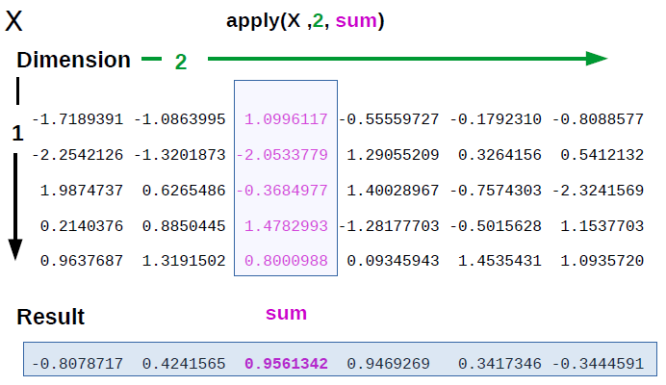
\includegraphics[width=4.16667in]{images/Apply_function.png}
\caption{apply}
\end{figure}

\begin{quote}
Заметьте, мы вставляем функцию без скобок и кавычек как аргумент в
функцию. Это как раз тот случай, когда аргументом в функции выступает
сама функция, а не ее название или результат ее выполнения.
\end{quote}

Давайте разберем на примере:

\begin{Shaded}
\begin{Highlighting}[]
\KeywordTok{apply}\NormalTok{(A, }\DecValTok{1}\NormalTok{, sum) }\CommentTok{#сумма по каждой строчке}
\end{Highlighting}
\end{Shaded}

\begin{verbatim}
## [1] 22 26 30
\end{verbatim}

\begin{Shaded}
\begin{Highlighting}[]
\KeywordTok{apply}\NormalTok{(A, }\DecValTok{2}\NormalTok{, sum) }\CommentTok{#сумма по каждой колонке}
\end{Highlighting}
\end{Shaded}

\begin{verbatim}
## [1]  6 15 24 33
\end{verbatim}

\begin{Shaded}
\begin{Highlighting}[]
\KeywordTok{apply}\NormalTok{(A, }\KeywordTok{c}\NormalTok{(}\DecValTok{1}\NormalTok{,}\DecValTok{2}\NormalTok{), sum) }\CommentTok{#кхм... сумма каждого элемента}
\end{Highlighting}
\end{Shaded}

\begin{verbatim}
##      [,1] [,2] [,3] [,4]
## [1,]    1    4    7   10
## [2,]    2    5    8   11
## [3,]    3    6    9   12
\end{verbatim}

\begin{quote}
Конкретно для подсчета сумм и средних по столбцам и строкам в R есть
функции \texttt{colSums()}, \texttt{rowSums()}, \texttt{colMeans()} и
\texttt{rowMeans()}, которые можно использовать как альтернативы
\texttt{apply()} в данном случае.
\end{quote}

Если же мы хотим прописать дополнительные аргументы для функции, то их
можно перечислить через запятую после функции:

\begin{Shaded}
\begin{Highlighting}[]
\KeywordTok{apply}\NormalTok{(A, }\DecValTok{1}\NormalTok{, sum, }\DataTypeTok{na.rm =} \OtherTok{TRUE}\NormalTok{)}
\end{Highlighting}
\end{Shaded}

\begin{verbatim}
## [1] 22 26 30
\end{verbatim}

\begin{Shaded}
\begin{Highlighting}[]
\KeywordTok{apply}\NormalTok{(A, }\DecValTok{1}\NormalTok{, weighted.mean, }\DataTypeTok{w =} \KeywordTok{c}\NormalTok{(}\FloatTok{0.2}\NormalTok{, }\FloatTok{0.4}\NormalTok{, }\FloatTok{0.3}\NormalTok{, }\FloatTok{0.1}\NormalTok{)) }
\end{Highlighting}
\end{Shaded}

\begin{verbatim}
## [1] 4.9 5.9 6.9
\end{verbatim}

\subsection{Анонимные функции}\label{anon_f}

Что делать, если мы хотим сделать что-то более сложное, чем просто
применить одну функцию? А если функция принимает не первым, а вторым
аргументом данные из матрицы? В этом случае нам помогут
\textbf{анонимные функции}.

Анонимные функции - это функции, которые будут использоваться один раз и
без названия.

\begin{quote}
Питонистам знакомо понятие \textbf{лямбда-функций}. Да, это то же самое.
\end{quote}

Например, мы можем посчитать отклонения от среднего без называния этой
функции:

\begin{Shaded}
\begin{Highlighting}[]
\KeywordTok{apply}\NormalTok{(A, }\DecValTok{1}\NormalTok{, }\ControlFlowTok{function}\NormalTok{(x) x }\OperatorTok{-}\StringTok{ }\KeywordTok{mean}\NormalTok{(x)) }\CommentTok{#отклонения от среднего по строчке}
\end{Highlighting}
\end{Shaded}

\begin{verbatim}
##      [,1] [,2] [,3]
## [1,] -4.5 -4.5 -4.5
## [2,] -1.5 -1.5 -1.5
## [3,]  1.5  1.5  1.5
## [4,]  4.5  4.5  4.5
\end{verbatim}

\begin{Shaded}
\begin{Highlighting}[]
\KeywordTok{apply}\NormalTok{(A, }\DecValTok{2}\NormalTok{, }\ControlFlowTok{function}\NormalTok{(x) x }\OperatorTok{-}\StringTok{ }\KeywordTok{mean}\NormalTok{(x)) }\CommentTok{#отклонения от среднего по столбцу}
\end{Highlighting}
\end{Shaded}

\begin{verbatim}
##      [,1] [,2] [,3] [,4]
## [1,]   -1   -1   -1   -1
## [2,]    0    0    0    0
## [3,]    1    1    1    1
\end{verbatim}

\begin{Shaded}
\begin{Highlighting}[]
\KeywordTok{apply}\NormalTok{(A, }\KeywordTok{c}\NormalTok{(}\DecValTok{1}\NormalTok{,}\DecValTok{2}\NormalTok{), }\ControlFlowTok{function}\NormalTok{(x) x }\OperatorTok{-}\StringTok{ }\KeywordTok{mean}\NormalTok{(x)) }\CommentTok{#отклонения от одного значения, т.е. ноль}
\end{Highlighting}
\end{Shaded}

\begin{verbatim}
##      [,1] [,2] [,3] [,4]
## [1,]    0    0    0    0
## [2,]    0    0    0    0
## [3,]    0    0    0    0
\end{verbatim}

Как и в случае с обычной функцией, в качестве \texttt{x} выступает
объект, с которым мы хотим что-то сделать, а дальше следует функция,
которую мы собираемся применить к \texttt{х}. Можно использовать не
\texttt{х}, а что угодно, как и в обычных функциях:

\begin{Shaded}
\begin{Highlighting}[]
\KeywordTok{apply}\NormalTok{(A, }\DecValTok{1}\NormalTok{, }\ControlFlowTok{function}\NormalTok{(whatevername) whatevername }\OperatorTok{-}\StringTok{ }\KeywordTok{mean}\NormalTok{(whatevername))}
\end{Highlighting}
\end{Shaded}

\begin{verbatim}
##      [,1] [,2] [,3]
## [1,] -4.5 -4.5 -4.5
## [2,] -1.5 -1.5 -1.5
## [3,]  1.5  1.5  1.5
## [4,]  4.5  4.5  4.5
\end{verbatim}

\subsection{\texorpdfstring{Другие функции семейства
\texttt{apply()}}{Другие функции семейства apply()}}\label{apply_other}

Ок, с \texttt{apply()} разобрались. А что с остальными? Некоторые из них
еще проще и не требуют индексов, например, \texttt{lapply} (для
применения к каждому элементу списка) и \texttt{sapply()} - упрощенная
версия \texttt{lapply()}, которая пытается по возможности ``упростить''
результат до вектора или матрицы.

\begin{Shaded}
\begin{Highlighting}[]
\NormalTok{some_list <-}\StringTok{ }\KeywordTok{list}\NormalTok{(}\DataTypeTok{some =} \DecValTok{1}\OperatorTok{:}\DecValTok{10}\NormalTok{, }\DataTypeTok{list =}\NormalTok{ letters)}
\KeywordTok{lapply}\NormalTok{(some_list, length)}
\end{Highlighting}
\end{Shaded}

\begin{verbatim}
## $some
## [1] 10
## 
## $list
## [1] 26
\end{verbatim}

\begin{Shaded}
\begin{Highlighting}[]
\KeywordTok{sapply}\NormalTok{(some_list, length)}
\end{Highlighting}
\end{Shaded}

\begin{verbatim}
## some list 
##   10   26
\end{verbatim}

Использование \texttt{sapply()} на векторе приводит к тем же
результатам, что и просто применить векторизованную функцию обычным
способом.

\begin{Shaded}
\begin{Highlighting}[]
\KeywordTok{sapply}\NormalTok{(}\DecValTok{1}\OperatorTok{:}\DecValTok{10}\NormalTok{, sqrt)}
\end{Highlighting}
\end{Shaded}

\begin{verbatim}
##  [1] 1.000000 1.414214 1.732051 2.000000 2.236068 2.449490 2.645751 2.828427
##  [9] 3.000000 3.162278
\end{verbatim}

\begin{Shaded}
\begin{Highlighting}[]
\KeywordTok{sqrt}\NormalTok{(}\DecValTok{1}\OperatorTok{:}\DecValTok{10}\NormalTok{)}
\end{Highlighting}
\end{Shaded}

\begin{verbatim}
##  [1] 1.000000 1.414214 1.732051 2.000000 2.236068 2.449490 2.645751 2.828427
##  [9] 3.000000 3.162278
\end{verbatim}

Зачем вообще тогда нужен \texttt{sapply()}, если мы можем просто
применить векторизованную функцию? Ключевое слово здесь
\emph{векторизованная} функция. Если функция не векторизована, то
\texttt{sapply()} становится удобным вариантом для того, чтобы избежать
итерирования с помощью циклов \texttt{for}.

\begin{quote}
Еще одна альтернатива - это векторизация невекторизованной функции с
помощью \texttt{Vectorize()}. Эта функция просто оборачивает функцию
одним из вариантов \texttt{apply()}.
\end{quote}

Можно применять функции \texttt{lapply()} и \texttt{sapply()} на
датафреймах. Поскольку фактически датафрейм - это список из векторов
одинаковой длины (см. \ref{df}), то итерироваться эти функции будут по
колонкам:

\begin{Shaded}
\begin{Highlighting}[]
\NormalTok{heroes <-}\StringTok{ }\KeywordTok{read.csv}\NormalTok{(}\StringTok{"data/heroes_information.csv"}\NormalTok{, }
                   \DataTypeTok{na.strings =} \KeywordTok{c}\NormalTok{(}\StringTok{"-"}\NormalTok{, }\StringTok{"-99"}\NormalTok{))}
\KeywordTok{sapply}\NormalTok{(heroes, class)}
\end{Highlighting}
\end{Shaded}

\begin{verbatim}
##           X        name      Gender   Eye.color        Race  Hair.color 
##   "integer" "character" "character" "character" "character" "character" 
##      Height   Publisher  Skin.color   Alignment      Weight 
##   "numeric" "character" "character" "character"   "integer"
\end{verbatim}

Еще одна функция из семейства \texttt{apply()} - функция
\texttt{replicate()} - самый простой способ повторить одну и ту же
операцию много раз. Обычно эта функция используется при симуляции данных
и моделировании. Например, давайте сделаем выборку из логнормального
распределения:

\begin{Shaded}
\begin{Highlighting}[]
\NormalTok{samp <-}\StringTok{ }\KeywordTok{rlnorm}\NormalTok{(}\DecValTok{30}\NormalTok{)}
\KeywordTok{hist}\NormalTok{(samp)}
\end{Highlighting}
\end{Shaded}

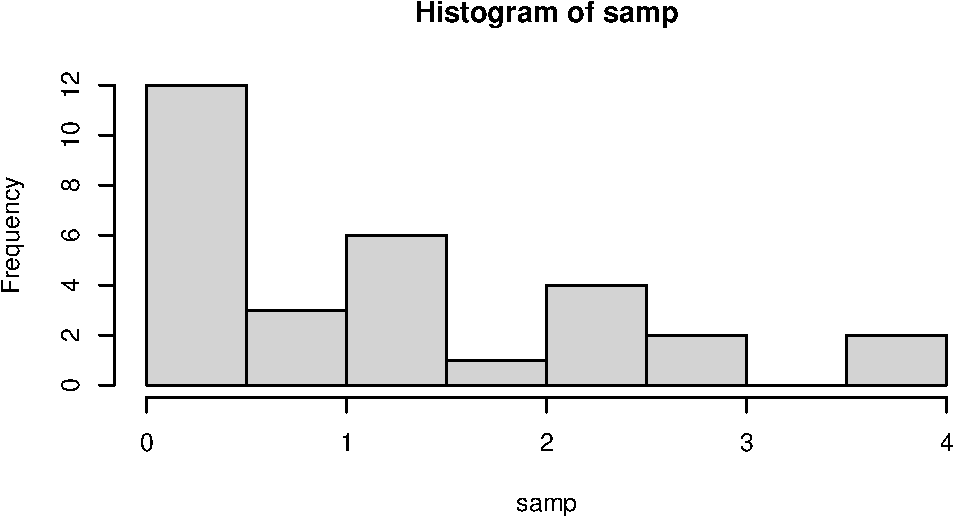
\includegraphics{tidy_stats_files/figure-latex/unnamed-chunk-170-1.pdf}

А теперь давайте сделаем 1000 таких выборок и из каждой возьмем среднее:

\begin{Shaded}
\begin{Highlighting}[]
\NormalTok{sampdist <-}\StringTok{ }\KeywordTok{replicate}\NormalTok{(}\DecValTok{1000}\NormalTok{, }\KeywordTok{mean}\NormalTok{(}\KeywordTok{rlnorm}\NormalTok{(}\DecValTok{30}\NormalTok{)))}
\KeywordTok{hist}\NormalTok{(sampdist)}
\end{Highlighting}
\end{Shaded}

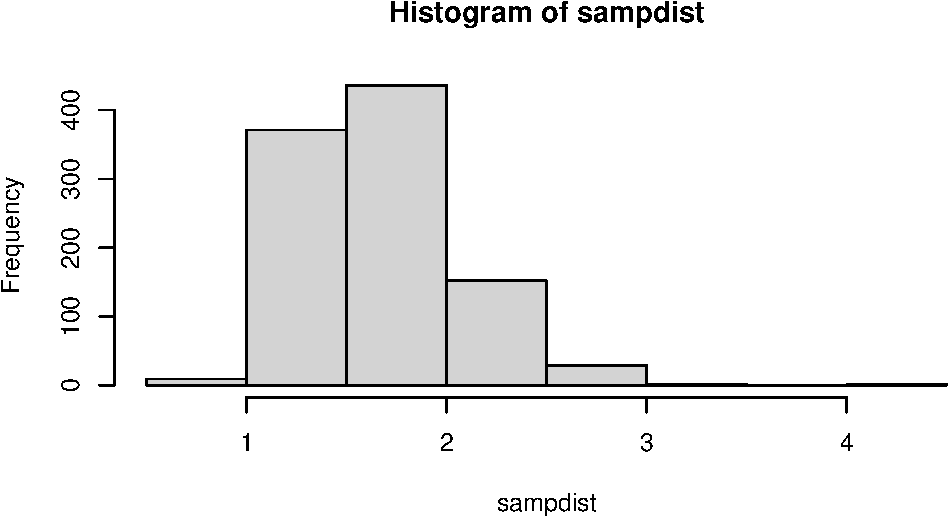
\includegraphics{tidy_stats_files/figure-latex/unnamed-chunk-171-1.pdf}

\begin{quote}
Про функции для генерации случайных чисел и про визуализацию мы
поговорим в следующие дни.
\end{quote}

Если хотите познакомиться с семейством \texttt{apply()} чуточку ближе,
то рекомендую
\href{https://www.datacamp.com/community/tutorials/r-tutorial-apply-family}{вот
этот туториал}.

В заключение стоит сказать, что семейство функций \texttt{apply()} ---
это очень сильное колдунство, но в tidyverse оно практически полностью
перекрывается функциями из пакета \texttt{purrr}. Впрочем, если вы
поняли логику \texttt{apply()}, то при желании вы легко сможете
переключиться на альтернативы из пакета \texttt{purrr}.

\chapter{Введение в tidyverse}\label{tidy_intro}

\section{Вселенная tidyverse}\label{tidy_verse}

tidyverse - это не один, а целое множество пакетов. Есть ключевые пакеты
(ядро тайдиверса), а есть побочные - в основном для работы со
специфическими видами данных.

\href{https://www.tidyverse.org}{\emph{tidyverse}} --- это набор
пакетов:

\begin{itemize}
\tightlist
\item
  \emph{ggplot2}, для визуализации
\item
  \emph{tibble}, для работы с тибблами, продвинутый вариант датафрейма
\item
  \emph{tidyr}, для формата tidy data
\item
  \emph{readr}, для чтения файлов в R
\item
  \emph{purrr}, для функционального программирования (замена семейства
  функций *apply())
\item
  \emph{dplyr}, для преобразованиия данных
\item
  \emph{stringr}, для работы со строковыми переменными
\item
  \emph{forcats}, для работы с переменными-факторами
\end{itemize}

Полезно также знать о следующих пакетах, не включенных в ядро, но также
считающихся частью тайдиверса:

\begin{itemize}
\tightlist
\item
  \emph{vroom}, для быстрой загрузки табоичных данных
\item
  \emph{readxl}, для чтения .xls и .xlsx
\item
  \emph{jsonlite}, для работы с JSON
\item
  \emph{xml}, для работы с XML
\item
  \emph{DBI}, для работы с базами данных
\item
  \emph{rvest}, для веб-скреппинга
\item
  \emph{lubridate}, для работы с временем
\item
  \emph{tidytext}, для работы с текстами и корпусами
\item
  \emph{glue}, для продвинутого объединения строк
\item
  \emph{magrtittr}, с несколькими вариантами pipe оператора
\item
  \emph{tidymodels}, для моделирования и машинного обучения\footnote{Как
    и пакет \texttt{tidyverse}, \texttt{tidymodels} --- это пакет с
    несколькими пакетами.}
\item
  \emph{dtplyr}, для ускорения \texttt{dplyr} за счет перевод синтаксиса
  на \texttt{data.table}
\end{itemize}

И это еще не все пакеты tidyverse! Есть еще много других небольших
пакетов, которые тоже считаются частью tidyverse. Кроме официальных
пакетов tidyverse есть множество пакетов, которые пытаются
соответствовать принципам tidyverse и дополняют его.

Все пакеты tidyverse объединены tidy философией и взаимосовместимым
синтаксисом. Это означает, что, во многих случаях даже не нужно думать о
том, из какого именно пакета тайдиверса пришла функция. Можно просто
установить и загрузить пакет \texttt{tidyverse}.

\begin{Shaded}
\begin{Highlighting}[]
\KeywordTok{install.packages}\NormalTok{(}\StringTok{"tidyverse"}\NormalTok{)}
\end{Highlighting}
\end{Shaded}

Пакет \texttt{tidyverse} --- это такой
\href{https://cs11.pikabu.ru/post_img/big/2019/03/12/11/1552415351186680692.jpg}{пакет
с пакетами}.

\begin{Shaded}
\begin{Highlighting}[]
\KeywordTok{library}\NormalTok{(}\StringTok{"tidyverse"}\NormalTok{)}
\end{Highlighting}
\end{Shaded}

\begin{verbatim}
## -- Attaching packages --------------------------------------- tidyverse 1.3.0 --
\end{verbatim}

\begin{verbatim}
## v ggplot2 3.3.2     v purrr   0.3.4
## v tibble  3.0.4     v dplyr   1.0.2
## v tidyr   1.1.2     v stringr 1.4.0
## v readr   1.4.0     v forcats 0.5.0
\end{verbatim}

\begin{verbatim}
## -- Conflicts ------------------------------------------ tidyverse_conflicts() --
## x dplyr::filter() masks stats::filter()
## x dplyr::lag()    masks stats::lag()
\end{verbatim}

Подключение пакета \texttt{tidyverse} автоматически приводит к
подключению ядра tidyverse, остальные же пакеты нужно подключать
дополнительно при необходимости.

\section{\texorpdfstring{Загрузка данных с помощью
\texttt{readr}}{Загрузка данных с помощью readr}}\label{ux437ux430ux433ux440ux443ux437ux43aux430-ux434ux430ux43dux43dux44bux445-ux441-ux43fux43eux43cux43eux449ux44cux44e-readr}

Стандартной функцией для чтения \texttt{.csv} файлов в R является
функция \texttt{read.csv()}, но мы будем использовать функцию
\texttt{read\_csv()} из пакета \texttt{readr}. Синтаксис функции
\texttt{read\_csv()} очень похож на \texttt{read.csv()}: первым
аргументом является путь к файлу (в том числе можно использовать URL),
некоторые остальные параметры тоже совпадают.

\begin{Shaded}
\begin{Highlighting}[]
\NormalTok{heroes <-}\StringTok{ }\KeywordTok{read_csv}\NormalTok{(}\StringTok{"data/heroes_information.csv"}\NormalTok{,}
                   \DataTypeTok{na =} \KeywordTok{c}\NormalTok{(}\StringTok{"-"}\NormalTok{, }\StringTok{"-99"}\NormalTok{))}
\end{Highlighting}
\end{Shaded}

\begin{verbatim}
## Warning: Missing column names filled in: 'X1' [1]
\end{verbatim}

\begin{verbatim}
## 
## -- Column specification --------------------------------------------------------
## cols(
##   X1 = col_double(),
##   name = col_character(),
##   Gender = col_character(),
##   `Eye color` = col_character(),
##   Race = col_character(),
##   `Hair color` = col_character(),
##   Height = col_double(),
##   Publisher = col_character(),
##   `Skin color` = col_character(),
##   Alignment = col_character(),
##   Weight = col_double()
## )
\end{verbatim}

Подробнее про импорт данных, в том числе в tidyverse, смотри в
@ref(real\_data).

\section{tibble}\label{tibble}

Когда мы загрузили данные с помощью \texttt{read\_csv()}, то мы получили
\texttt{tibble}, а не \texttt{data.frame}:

\begin{Shaded}
\begin{Highlighting}[]
\KeywordTok{class}\NormalTok{(heroes)}
\end{Highlighting}
\end{Shaded}

\begin{verbatim}
## [1] "spec_tbl_df" "tbl_df"      "tbl"         "data.frame"
\end{verbatim}

Тиббл (\texttt{tibble}) - это такой ``усовершенствованный''
\texttt{data.frame}.
\href{https://www.jumpingrivers.com/blog/the-trouble-with-tibbles/}{Почти}
все, что работает с \texttt{data.frame}, работает и с тибблами. Однако у
тибблов есть свои дополнительные фишки. Самая очевидная из них - более
аккуратный вывод в консоль:

\begin{Shaded}
\begin{Highlighting}[]
\NormalTok{heroes}
\end{Highlighting}
\end{Shaded}

\begin{verbatim}
## # A tibble: 734 x 11
##       X1 name  Gender `Eye color` Race  `Hair color` Height Publisher
##    <dbl> <chr> <chr>  <chr>       <chr> <chr>         <dbl> <chr>    
##  1     0 A-Bo~ Male   yellow      Human No Hair         203 Marvel C~
##  2     1 Abe ~ Male   blue        Icth~ No Hair         191 Dark Hor~
##  3     2 Abin~ Male   blue        Unga~ No Hair         185 DC Comics
##  4     3 Abom~ Male   green       Huma~ No Hair         203 Marvel C~
##  5     4 Abra~ Male   blue        Cosm~ Black            NA Marvel C~
##  6     5 Abso~ Male   blue        Human No Hair         193 Marvel C~
##  7     6 Adam~ Male   blue        <NA>  Blond            NA NBC - He~
##  8     7 Adam~ Male   blue        Human Blond           185 DC Comics
##  9     8 Agen~ Female blue        <NA>  Blond           173 Marvel C~
## 10     9 Agen~ Male   brown       Human Brown           178 Marvel C~
## # ... with 724 more rows, and 3 more variables: `Skin color` <chr>,
## #   Alignment <chr>, Weight <dbl>
\end{verbatim}

Выводятся только первые 10 строк, если какие-то колонки не влезают на
экран, то они просто перечислены внизу. Ну а тип данных написан прямо
под названием колонки.

Функции различных пакетов tidyverse сами конвертируют в тиббл при
необходимости. Если же нужно это сделать самостоятельно, то можно это
сделать так:

\begin{Shaded}
\begin{Highlighting}[]
\NormalTok{heroes_df <-}\StringTok{ }\KeywordTok{as.data.frame}\NormalTok{(heroes) }\CommentTok{#создаем простой датафрейм}
\KeywordTok{class}\NormalTok{(heroes_df)}
\end{Highlighting}
\end{Shaded}

\begin{verbatim}
## [1] "data.frame"
\end{verbatim}

\begin{Shaded}
\begin{Highlighting}[]
\KeywordTok{as_tibble}\NormalTok{(heroes_df) }\CommentTok{#превращаем обратно в тиббл}
\end{Highlighting}
\end{Shaded}

\begin{verbatim}
## # A tibble: 734 x 11
##       X1 name  Gender `Eye color` Race  `Hair color` Height Publisher
##    <dbl> <chr> <chr>  <chr>       <chr> <chr>         <dbl> <chr>    
##  1     0 A-Bo~ Male   yellow      Human No Hair         203 Marvel C~
##  2     1 Abe ~ Male   blue        Icth~ No Hair         191 Dark Hor~
##  3     2 Abin~ Male   blue        Unga~ No Hair         185 DC Comics
##  4     3 Abom~ Male   green       Huma~ No Hair         203 Marvel C~
##  5     4 Abra~ Male   blue        Cosm~ Black            NA Marvel C~
##  6     5 Abso~ Male   blue        Human No Hair         193 Marvel C~
##  7     6 Adam~ Male   blue        <NA>  Blond            NA NBC - He~
##  8     7 Adam~ Male   blue        Human Blond           185 DC Comics
##  9     8 Agen~ Female blue        <NA>  Blond           173 Marvel C~
## 10     9 Agen~ Male   brown       Human Brown           178 Marvel C~
## # ... with 724 more rows, and 3 more variables: `Skin color` <chr>,
## #   Alignment <chr>, Weight <dbl>
\end{verbatim}

\begin{quote}
В дальнейшем мы будем работать только с tidyverse, а это значит, что
только с тибблами, а не обычными датафреймами. Тем не менее, тибблы и
датафреймы будут в дальнейшем использоваться как синонимы.
\end{quote}

Можно создавать тибблы вручную с помощью функции \texttt{tibble()},
которая работает аналогично функции \texttt{data.frame()}:

\begin{Shaded}
\begin{Highlighting}[]
\KeywordTok{tibble}\NormalTok{(}
  \DataTypeTok{a =} \DecValTok{1}\OperatorTok{:}\DecValTok{3}\NormalTok{,}
  \DataTypeTok{b =}\NormalTok{ letters[}\DecValTok{1}\OperatorTok{:}\DecValTok{3}\NormalTok{]}
\NormalTok{)}
\end{Highlighting}
\end{Shaded}

\begin{verbatim}
## # A tibble: 3 x 2
##       a b    
##   <int> <chr>
## 1     1 a    
## 2     2 b    
## 3     3 c
\end{verbatim}

\section{\texorpdfstring{magrittr::\texttt{\%\textgreater{}\%}}{magrittr::\%\textgreater{}\%}}\label{pipe}

Оператор \texttt{\%\textgreater{}\%} называется ``пайпом'' (pipe), т.е.
``трубой''. Он означает, что следующая функция (справа от пайпа)
принимает на вход в качестве первого аргумента результат выполнения
предыдущей функции (той, что слева). Фактически, это примерно то же
самое, что и вставлять результат выполнения функции в качестве первого
аргумента в другую функцию. Просто выглядит это красивее и читабельнее.
Как будто данные пропускаются через трубы функций или конвеерную ленту
на заводе, если хотите. А то, что первый параметр функции - это почти
всегда данные, работает нам здесь на руку. Этот оператор взят из пакета
\texttt{magrittr}\footnote{Если быть точным, то оператор
  \texttt{\%\textgreater{}\%} был импортирован во все основные пакеты
  tidyverse, а сам пакет \texttt{magrittr} не входит в базовый набор
  tidyverse. Тем не менее, в самом \texttt{magrittr} есть еще несколько
  интересных операторов.}. Возможно, даже если вы не захотите
пользоваться tidyverse, использование пайпов Вам понравится.

Важно понимать, что пайп не дает какой-то дополнительной
функциональности или дополнительной скорости работы\footnote{Даже
  наоборот, использование пайпов незначительно снижает скорость
  выполнения команды.}. Он создан исключительно для читабельности и
комфорта.

С помощью пайпов вот эту команду\ldots{}

\begin{Shaded}
\begin{Highlighting}[]
\KeywordTok{sum}\NormalTok{(}\KeywordTok{sqrt}\NormalTok{(}\KeywordTok{abs}\NormalTok{(}\KeywordTok{sin}\NormalTok{(}\DecValTok{1}\OperatorTok{:}\DecValTok{22}\NormalTok{))))}
\end{Highlighting}
\end{Shaded}

\begin{verbatim}
## [1] 16.72656
\end{verbatim}

\ldots{}можно переписать вот так:

\begin{Shaded}
\begin{Highlighting}[]
\DecValTok{1}\OperatorTok{:}\DecValTok{22} \OperatorTok\StringTok{ }
\StringTok{  }\KeywordTok{sin}\NormalTok{() }\OperatorTok\StringTok{ }
\StringTok{  }\KeywordTok{abs}\NormalTok{() }\OperatorTok\StringTok{ }
\StringTok{  }\KeywordTok{sqrt}\NormalTok{() }\OperatorTok\StringTok{ }
\StringTok{  }\KeywordTok{sum}\NormalTok{()}
\end{Highlighting}
\end{Shaded}

\begin{verbatim}
## [1] 16.72656
\end{verbatim}

В очень редких случаях результат выполнения функции нужно вставить не на
первую позицию (или же мы хотим использовать его несколько раз). В этих
случаях можно использовать \texttt{.}, чтобы обозначить, куда мы хотим
вставить результат выполнения выражения слева от
\texttt{\%\textgreater{}\%}.

\begin{Shaded}
\begin{Highlighting}[]
\StringTok{"Всем привет!"} \OperatorTok
\StringTok{  }\KeywordTok{c}\NormalTok{(}\StringTok{"--"}\NormalTok{, ., }\StringTok{"--"}\NormalTok{)}
\end{Highlighting}
\end{Shaded}

\begin{verbatim}
## [1] "--"           "Всем привет!" "--"
\end{verbatim}

\section{\texorpdfstring{Главные пакеты tidyverse: \texttt{dplyr} и
\texttt{tidyr}}{Главные пакеты tidyverse: dplyr и tidyr}}\label{ux433ux43bux430ux432ux43dux44bux435-ux43fux430ux43aux435ux442ux44b-tidyverse-dplyr-ux438-tidyr}

\texttt{dplyr}\footnote{\href{https://community.rstudio.com/t/pronunciations-of-common-r-terms/1810}{Есть
  споры о том, как это правильно читать}. Используемые варианты:
  \emph{диплаер}, \emph{диплюр}, \emph{диплир}.} --- это самая основа
всего \texttt{tidyverse}. Этот пакет предоставляет основные функции для
манипуляции с тибблами. Пакет \texttt{dplyr} является наследником и
более усовершенствованной версией \texttt{plyr}, так что если увидите
использование пакета \texttt{plyr}, то, скорее всего, скрипт был написан
очень давно.

Пакет \texttt{tidyr} дополняет \texttt{dplyr}, предоставляя полезные
функции для тайдификации тибблов. Тайдификация (``аккуратизация'')
данных означает приведение табличных данных к такому формату, в котором:

\begin{itemize}
\tightlist
\item
  Каждая переменная имеет собственный столбец
\item
  Каждый наблюдение имеет собственную строку
\item
  Каждое значение имеет свою собственную ячейку
\end{itemize}

Впрочем, многие функции \texttt{dplyr} часто используются при
тайдификации, так же как и многие функции \texttt{tidyr} имеет
применение вне тайдификации. В общем, функционал этих двух пакетов
несколько смешался, поэтому мы будем рассматривать их вместе. А чтобы
представлять, какая функция относится к какому пакету (хотя запоминать
это необязательно), я буду использовать запись с двумя двоеточиями
\texttt{::}, которая обычно используется для использования функции без
подгрузки всего пакета, при первом упоминании функции.

Пакет \texttt{tidyr} --- это более усовершенствованная версия пакета
\texttt{reshape2}, который в свою очередь является усовершенствованной
версией \texttt{reshape}. По аналогии с \texttt{plyr}, если вы видите
использование этих пакетов, то это указывает на то, что перед вами
морально устаревший код.

Код с использованием \texttt{dplyr} и \texttt{tidyr}сильно непохож на
то, что мы видели раньше. Большинство функций \texttt{dplyr} и
\texttt{tidyr} работают с целым тибблом сразу, принимая его в качестве
первого аргумента и возвращая измененный тиббл. Это позволяет превратить
весь код в последовательный набор применяемых функций, соединенный
пайпами. На практике это выглядит очень элегантно, и вы в этом скоро
убедитесь.

\section{Работа с колонками тиббла}\label{tidy_select_cols}

\subsection{\texorpdfstring{Выбор колонок:
\texttt{dplyr::select()}}{Выбор колонок: dplyr::select()}}\label{ux432ux44bux431ux43eux440-ux43aux43eux43bux43eux43dux43eux43a-dplyrselect}

Функция \texttt{dplyr::select()} позволяет выбирать колонки по номеру
или имени (кавычки не нужны).

\begin{Shaded}
\begin{Highlighting}[]
\NormalTok{heroes }\OperatorTok
\StringTok{  }\KeywordTok{select}\NormalTok{(}\DecValTok{1}\NormalTok{,}\DecValTok{5}\NormalTok{)}
\end{Highlighting}
\end{Shaded}

\begin{verbatim}
## # A tibble: 734 x 2
##       X1 Race             
##    <dbl> <chr>            
##  1     0 Human            
##  2     1 Icthyo Sapien    
##  3     2 Ungaran          
##  4     3 Human / Radiation
##  5     4 Cosmic Entity    
##  6     5 Human            
##  7     6 <NA>             
##  8     7 Human            
##  9     8 <NA>             
## 10     9 Human            
## # ... with 724 more rows
\end{verbatim}

\begin{Shaded}
\begin{Highlighting}[]
\NormalTok{heroes }\OperatorTok
\StringTok{  }\KeywordTok{select}\NormalTok{(name, Race, Publisher, }\StringTok{`}\DataTypeTok{Hair color}\StringTok{`}\NormalTok{)}
\end{Highlighting}
\end{Shaded}

\begin{verbatim}
## # A tibble: 734 x 4
##    name          Race              Publisher         `Hair color`
##    <chr>         <chr>             <chr>             <chr>       
##  1 A-Bomb        Human             Marvel Comics     No Hair     
##  2 Abe Sapien    Icthyo Sapien     Dark Horse Comics No Hair     
##  3 Abin Sur      Ungaran           DC Comics         No Hair     
##  4 Abomination   Human / Radiation Marvel Comics     No Hair     
##  5 Abraxas       Cosmic Entity     Marvel Comics     Black       
##  6 Absorbing Man Human             Marvel Comics     No Hair     
##  7 Adam Monroe   <NA>              NBC - Heroes      Blond       
##  8 Adam Strange  Human             DC Comics         Blond       
##  9 Agent 13      <NA>              Marvel Comics     Blond       
## 10 Agent Bob     Human             Marvel Comics     Brown       
## # ... with 724 more rows
\end{verbatim}

Обратите внимание, если в названии колонки присутствует пробел или,
например, колонка начинается с цифры или точки и цифры, то это
синтаксически невалидное имя (\ref{variables}). Это не значит, что такие
названия колонок недопустимы. Но такие названия колонок нужно обособлять
` грависом (правый штрих, на клавиатуре находится там же где и буква ё и
\textasciitilde{}).

Еще обратите внимание на то, что функции tidyverse не изменяют сами
изначальные тибблы/датафреймы. Это означает, что если вы хотите
полученный результат сохранить, то нужно добавить присвоение:

\begin{Shaded}
\begin{Highlighting}[]
\NormalTok{heroes_some_cols <-}\StringTok{ }\NormalTok{heroes }\OperatorTok
\StringTok{  }\KeywordTok{select}\NormalTok{(name, Race, Publisher, }\StringTok{`}\DataTypeTok{Hair color}\StringTok{`}\NormalTok{)}
\NormalTok{heroes_some_cols}
\end{Highlighting}
\end{Shaded}

\begin{verbatim}
## # A tibble: 734 x 4
##    name          Race              Publisher         `Hair color`
##    <chr>         <chr>             <chr>             <chr>       
##  1 A-Bomb        Human             Marvel Comics     No Hair     
##  2 Abe Sapien    Icthyo Sapien     Dark Horse Comics No Hair     
##  3 Abin Sur      Ungaran           DC Comics         No Hair     
##  4 Abomination   Human / Radiation Marvel Comics     No Hair     
##  5 Abraxas       Cosmic Entity     Marvel Comics     Black       
##  6 Absorbing Man Human             Marvel Comics     No Hair     
##  7 Adam Monroe   <NA>              NBC - Heroes      Blond       
##  8 Adam Strange  Human             DC Comics         Blond       
##  9 Agent 13      <NA>              Marvel Comics     Blond       
## 10 Agent Bob     Human             Marvel Comics     Brown       
## # ... with 724 more rows
\end{verbatim}

\subsection{Мини-язык tidyselect для выбора колонок}\label{tidyselect}

Для выбора столбцов (не только в \texttt{select()}, но и для других
функций tidyverse) используется специальный мини-язык tidyselect из
одноименного пакета\footnote{Как и в случае с \texttt{magrittr}, пакет
  \texttt{tidyselect} не содержатся в базовом tidyverse, но функции
  импортируются основыми пакетами tidyverse.}. tidyselect дает очень
широкие возможности для выбора колонок.

Можно использовать оператор \texttt{:} для выбора нескольких соседних
колонок (по аналогии с созданием числового вектора с шагом 1).

\begin{Shaded}
\begin{Highlighting}[]
\NormalTok{heroes }\OperatorTok
\StringTok{  }\KeywordTok{select}\NormalTok{(name}\OperatorTok{:}\NormalTok{Publisher)}
\end{Highlighting}
\end{Shaded}

\begin{verbatim}
## # A tibble: 734 x 7
##    name       Gender `Eye color` Race          `Hair color` Height Publisher    
##    <chr>      <chr>  <chr>       <chr>         <chr>         <dbl> <chr>        
##  1 A-Bomb     Male   yellow      Human         No Hair         203 Marvel Comics
##  2 Abe Sapien Male   blue        Icthyo Sapien No Hair         191 Dark Horse C~
##  3 Abin Sur   Male   blue        Ungaran       No Hair         185 DC Comics    
##  4 Abominati~ Male   green       Human / Radi~ No Hair         203 Marvel Comics
##  5 Abraxas    Male   blue        Cosmic Entity Black            NA Marvel Comics
##  6 Absorbing~ Male   blue        Human         No Hair         193 Marvel Comics
##  7 Adam Monr~ Male   blue        <NA>          Blond            NA NBC - Heroes 
##  8 Adam Stra~ Male   blue        Human         Blond           185 DC Comics    
##  9 Agent 13   Female blue        <NA>          Blond           173 Marvel Comics
## 10 Agent Bob  Male   brown       Human         Brown           178 Marvel Comics
## # ... with 724 more rows
\end{verbatim}

\begin{Shaded}
\begin{Highlighting}[]
\NormalTok{heroes }\OperatorTok
\StringTok{  }\KeywordTok{select}\NormalTok{(name}\OperatorTok{:}\StringTok{`}\DataTypeTok{Eye color}\StringTok{`}\NormalTok{, Publisher}\OperatorTok{:}\NormalTok{Weight)}
\end{Highlighting}
\end{Shaded}

\begin{verbatim}
## # A tibble: 734 x 7
##    name         Gender `Eye color` Publisher       `Skin color` Alignment Weight
##    <chr>        <chr>  <chr>       <chr>           <chr>        <chr>      <dbl>
##  1 A-Bomb       Male   yellow      Marvel Comics   <NA>         good         441
##  2 Abe Sapien   Male   blue        Dark Horse Com~ blue         good          65
##  3 Abin Sur     Male   blue        DC Comics       red          good          90
##  4 Abomination  Male   green       Marvel Comics   <NA>         bad          441
##  5 Abraxas      Male   blue        Marvel Comics   <NA>         bad           NA
##  6 Absorbing M~ Male   blue        Marvel Comics   <NA>         bad          122
##  7 Adam Monroe  Male   blue        NBC - Heroes    <NA>         good          NA
##  8 Adam Strange Male   blue        DC Comics       <NA>         good          88
##  9 Agent 13     Female blue        Marvel Comics   <NA>         good          61
## 10 Agent Bob    Male   brown       Marvel Comics   <NA>         good          81
## # ... with 724 more rows
\end{verbatim}

Используя \texttt{!} можно вырезать ненужные колонки.

\begin{Shaded}
\begin{Highlighting}[]
\NormalTok{heroes }\OperatorTok
\StringTok{  }\KeywordTok{select}\NormalTok{(}\OperatorTok{!}\NormalTok{X1)}
\end{Highlighting}
\end{Shaded}

\begin{verbatim}
## # A tibble: 734 x 10
##    name  Gender `Eye color` Race  `Hair color` Height Publisher `Skin color`
##    <chr> <chr>  <chr>       <chr> <chr>         <dbl> <chr>     <chr>       
##  1 A-Bo~ Male   yellow      Human No Hair         203 Marvel C~ <NA>        
##  2 Abe ~ Male   blue        Icth~ No Hair         191 Dark Hor~ blue        
##  3 Abin~ Male   blue        Unga~ No Hair         185 DC Comics red         
##  4 Abom~ Male   green       Huma~ No Hair         203 Marvel C~ <NA>        
##  5 Abra~ Male   blue        Cosm~ Black            NA Marvel C~ <NA>        
##  6 Abso~ Male   blue        Human No Hair         193 Marvel C~ <NA>        
##  7 Adam~ Male   blue        <NA>  Blond            NA NBC - He~ <NA>        
##  8 Adam~ Male   blue        Human Blond           185 DC Comics <NA>        
##  9 Agen~ Female blue        <NA>  Blond           173 Marvel C~ <NA>        
## 10 Agen~ Male   brown       Human Brown           178 Marvel C~ <NA>        
## # ... with 724 more rows, and 2 more variables: Alignment <chr>, Weight <dbl>
\end{verbatim}

\begin{Shaded}
\begin{Highlighting}[]
\NormalTok{heroes }\OperatorTok
\StringTok{  }\KeywordTok{select}\NormalTok{(}\OperatorTok{!}\NormalTok{(Gender}\OperatorTok{:}\NormalTok{Height))}
\end{Highlighting}
\end{Shaded}

\begin{verbatim}
## # A tibble: 734 x 6
##       X1 name          Publisher         `Skin color` Alignment Weight
##    <dbl> <chr>         <chr>             <chr>        <chr>      <dbl>
##  1     0 A-Bomb        Marvel Comics     <NA>         good         441
##  2     1 Abe Sapien    Dark Horse Comics blue         good          65
##  3     2 Abin Sur      DC Comics         red          good          90
##  4     3 Abomination   Marvel Comics     <NA>         bad          441
##  5     4 Abraxas       Marvel Comics     <NA>         bad           NA
##  6     5 Absorbing Man Marvel Comics     <NA>         bad          122
##  7     6 Adam Monroe   NBC - Heroes      <NA>         good          NA
##  8     7 Adam Strange  DC Comics         <NA>         good          88
##  9     8 Agent 13      Marvel Comics     <NA>         good          61
## 10     9 Agent Bob     Marvel Comics     <NA>         good          81
## # ... with 724 more rows
\end{verbatim}

Другие известные нам логические операторы (\texttt{\&} и
\texttt{\textbar{}}) тоже работают в tidyselect.

В дополнение к логическим операторам и \texttt{:}, в tidyselect есть
набор вспомогательных функций, работающих исключительно в контексте
выбора колонок с помощью tidyselect.

Вспомогательная функция \texttt{last\_col()} позволит обратиться к
последней колонке тиббла:

\begin{Shaded}
\begin{Highlighting}[]
\NormalTok{heroes }\OperatorTok
\StringTok{  }\KeywordTok{select}\NormalTok{(name}\OperatorTok{:}\KeywordTok{last_col}\NormalTok{())}
\end{Highlighting}
\end{Shaded}

\begin{verbatim}
## # A tibble: 734 x 10
##    name  Gender `Eye color` Race  `Hair color` Height Publisher `Skin color`
##    <chr> <chr>  <chr>       <chr> <chr>         <dbl> <chr>     <chr>       
##  1 A-Bo~ Male   yellow      Human No Hair         203 Marvel C~ <NA>        
##  2 Abe ~ Male   blue        Icth~ No Hair         191 Dark Hor~ blue        
##  3 Abin~ Male   blue        Unga~ No Hair         185 DC Comics red         
##  4 Abom~ Male   green       Huma~ No Hair         203 Marvel C~ <NA>        
##  5 Abra~ Male   blue        Cosm~ Black            NA Marvel C~ <NA>        
##  6 Abso~ Male   blue        Human No Hair         193 Marvel C~ <NA>        
##  7 Adam~ Male   blue        <NA>  Blond            NA NBC - He~ <NA>        
##  8 Adam~ Male   blue        Human Blond           185 DC Comics <NA>        
##  9 Agen~ Female blue        <NA>  Blond           173 Marvel C~ <NA>        
## 10 Agen~ Male   brown       Human Brown           178 Marvel C~ <NA>        
## # ... with 724 more rows, and 2 more variables: Alignment <chr>, Weight <dbl>
\end{verbatim}

А функция \texttt{everything()} позволяет выбрать все колонки.

\begin{Shaded}
\begin{Highlighting}[]
\NormalTok{heroes }\OperatorTok
\StringTok{  }\KeywordTok{select}\NormalTok{(}\KeywordTok{everything}\NormalTok{())}
\end{Highlighting}
\end{Shaded}

\begin{verbatim}
## # A tibble: 734 x 11
##       X1 name  Gender `Eye color` Race  `Hair color` Height Publisher
##    <dbl> <chr> <chr>  <chr>       <chr> <chr>         <dbl> <chr>    
##  1     0 A-Bo~ Male   yellow      Human No Hair         203 Marvel C~
##  2     1 Abe ~ Male   blue        Icth~ No Hair         191 Dark Hor~
##  3     2 Abin~ Male   blue        Unga~ No Hair         185 DC Comics
##  4     3 Abom~ Male   green       Huma~ No Hair         203 Marvel C~
##  5     4 Abra~ Male   blue        Cosm~ Black            NA Marvel C~
##  6     5 Abso~ Male   blue        Human No Hair         193 Marvel C~
##  7     6 Adam~ Male   blue        <NA>  Blond            NA NBC - He~
##  8     7 Adam~ Male   blue        Human Blond           185 DC Comics
##  9     8 Agen~ Female blue        <NA>  Blond           173 Marvel C~
## 10     9 Agen~ Male   brown       Human Brown           178 Marvel C~
## # ... with 724 more rows, and 3 more variables: `Skin color` <chr>,
## #   Alignment <chr>, Weight <dbl>
\end{verbatim}

При этом \texttt{everything()} не будет дублировать выбранные колонки,
поэтому можно использовать \texttt{everything()} для перестановки
колонок в тиббле:

\begin{Shaded}
\begin{Highlighting}[]
\NormalTok{heroes }\OperatorTok
\StringTok{  }\KeywordTok{select}\NormalTok{(name, Publisher, }\KeywordTok{everything}\NormalTok{())}
\end{Highlighting}
\end{Shaded}

\begin{verbatim}
## # A tibble: 734 x 11
##    name  Publisher    X1 Gender `Eye color` Race  `Hair color` Height
##    <chr> <chr>     <dbl> <chr>  <chr>       <chr> <chr>         <dbl>
##  1 A-Bo~ Marvel C~     0 Male   yellow      Human No Hair         203
##  2 Abe ~ Dark Hor~     1 Male   blue        Icth~ No Hair         191
##  3 Abin~ DC Comics     2 Male   blue        Unga~ No Hair         185
##  4 Abom~ Marvel C~     3 Male   green       Huma~ No Hair         203
##  5 Abra~ Marvel C~     4 Male   blue        Cosm~ Black            NA
##  6 Abso~ Marvel C~     5 Male   blue        Human No Hair         193
##  7 Adam~ NBC - He~     6 Male   blue        <NA>  Blond            NA
##  8 Adam~ DC Comics     7 Male   blue        Human Blond           185
##  9 Agen~ Marvel C~     8 Female blue        <NA>  Blond           173
## 10 Agen~ Marvel C~     9 Male   brown       Human Brown           178
## # ... with 724 more rows, and 3 more variables: `Skin color` <chr>,
## #   Alignment <chr>, Weight <dbl>
\end{verbatim}

Впрочем, для перестановки колонок удобнее использовать специальную
функцию \texttt{relocate()} (@ref(tidy\_relocate)) Можно даже выбирать
колонки по паттернам в названиях. Например, с помощью
\texttt{ends\_with()} можно выбрать все колонки, заканчивающиеся
одинаковым суффиксом:

\begin{Shaded}
\begin{Highlighting}[]
\NormalTok{heroes }\OperatorTok
\StringTok{  }\KeywordTok{select}\NormalTok{(}\KeywordTok{ends_with}\NormalTok{(}\StringTok{"color"}\NormalTok{))}
\end{Highlighting}
\end{Shaded}

\begin{verbatim}
## # A tibble: 734 x 3
##    `Eye color` `Hair color` `Skin color`
##    <chr>       <chr>        <chr>       
##  1 yellow      No Hair      <NA>        
##  2 blue        No Hair      blue        
##  3 blue        No Hair      red         
##  4 green       No Hair      <NA>        
##  5 blue        Black        <NA>        
##  6 blue        No Hair      <NA>        
##  7 blue        Blond        <NA>        
##  8 blue        Blond        <NA>        
##  9 blue        Blond        <NA>        
## 10 brown       Brown        <NA>        
## # ... with 724 more rows
\end{verbatim}

Аналогично, с помощью функции \texttt{starts\_with()} можно найти
колонки с одинаковым префиксом, с помощью \texttt{contains()} --- все
колонки с выбранным паттерном в любой части названия колонки\footnote{Выбранный
  паттерн будет найден посимвольно, если же вы хотите искать по
  регулярным выражениям, то вместо \texttt{contains()} нужно
  использовать \texttt{matches()}.}.

\begin{Shaded}
\begin{Highlighting}[]
\NormalTok{heroes }\OperatorTok
\StringTok{  }\KeywordTok{select}\NormalTok{(}\KeywordTok{starts_with}\NormalTok{(}\StringTok{"Eye"}\NormalTok{) }\OperatorTok{&}\StringTok{ }\KeywordTok{ends_with}\NormalTok{(}\StringTok{"color"}\NormalTok{))}
\end{Highlighting}
\end{Shaded}

\begin{verbatim}
## # A tibble: 734 x 1
##    `Eye color`
##    <chr>      
##  1 yellow     
##  2 blue       
##  3 blue       
##  4 green      
##  5 blue       
##  6 blue       
##  7 blue       
##  8 blue       
##  9 blue       
## 10 brown      
## # ... with 724 more rows
\end{verbatim}

\begin{Shaded}
\begin{Highlighting}[]
\NormalTok{heroes }\OperatorTok
\StringTok{  }\KeywordTok{select}\NormalTok{(}\KeywordTok{contains}\NormalTok{(}\StringTok{"eight"}\NormalTok{))}
\end{Highlighting}
\end{Shaded}

\begin{verbatim}
## # A tibble: 734 x 2
##    Height Weight
##     <dbl>  <dbl>
##  1    203    441
##  2    191     65
##  3    185     90
##  4    203    441
##  5     NA     NA
##  6    193    122
##  7     NA     NA
##  8    185     88
##  9    173     61
## 10    178     81
## # ... with 724 more rows
\end{verbatim}

Ну и наконец, можно выбирать по содержимому колонок с помощью
\texttt{where()}. Это напоминает применение
\texttt{sapply()}(@ref(apply\_other)) на датафрейме для индексирования
колонок: в качестве аргумента для \texttt{where} принимается функция,
которая применяется для каждой из колонок, после чего выбираются только
те колонки, для которых было получено \texttt{TRUE}.

\begin{Shaded}
\begin{Highlighting}[]
\NormalTok{heroes }\OperatorTok
\StringTok{  }\KeywordTok{select}\NormalTok{(}\KeywordTok{where}\NormalTok{(is.numeric))}
\end{Highlighting}
\end{Shaded}

\begin{verbatim}
## # A tibble: 734 x 3
##       X1 Height Weight
##    <dbl>  <dbl>  <dbl>
##  1     0    203    441
##  2     1    191     65
##  3     2    185     90
##  4     3    203    441
##  5     4     NA     NA
##  6     5    193    122
##  7     6     NA     NA
##  8     7    185     88
##  9     8    173     61
## 10     9    178     81
## # ... with 724 more rows
\end{verbatim}

Функция \texttt{where()} дает невиданную мощь. Например, можно выбрать
все колонки без \texttt{NA}:

\begin{Shaded}
\begin{Highlighting}[]
\NormalTok{heroes }\OperatorTok
\StringTok{  }\KeywordTok{select}\NormalTok{(}\KeywordTok{where}\NormalTok{(}\ControlFlowTok{function}\NormalTok{(x) }\OperatorTok{!}\KeywordTok{any}\NormalTok{(}\KeywordTok{is.na}\NormalTok{(x))))}
\end{Highlighting}
\end{Shaded}

\begin{verbatim}
## # A tibble: 734 x 3
##       X1 name          Publisher        
##    <dbl> <chr>         <chr>            
##  1     0 A-Bomb        Marvel Comics    
##  2     1 Abe Sapien    Dark Horse Comics
##  3     2 Abin Sur      DC Comics        
##  4     3 Abomination   Marvel Comics    
##  5     4 Abraxas       Marvel Comics    
##  6     5 Absorbing Man Marvel Comics    
##  7     6 Adam Monroe   NBC - Heroes     
##  8     7 Adam Strange  DC Comics        
##  9     8 Agent 13      Marvel Comics    
## 10     9 Agent Bob     Marvel Comics    
## # ... with 724 more rows
\end{verbatim}

\subsection{\texorpdfstring{Переименование колонок:
\texttt{dplyr::rename()}}{Переименование колонок: dplyr::rename()}}\label{ux43fux435ux440ux435ux438ux43cux435ux43dux43eux432ux430ux43dux438ux435-ux43aux43eux43bux43eux43dux43eux43a-dplyrrename}

Внутри \texttt{select()} можно не только выбирать колонки, но и
переименовывать их:

\begin{Shaded}
\begin{Highlighting}[]
\NormalTok{heroes }\OperatorTok
\StringTok{  }\KeywordTok{select}\NormalTok{(}\DataTypeTok{id =}\NormalTok{ X1)}
\end{Highlighting}
\end{Shaded}

\begin{verbatim}
## # A tibble: 734 x 1
##       id
##    <dbl>
##  1     0
##  2     1
##  3     2
##  4     3
##  5     4
##  6     5
##  7     6
##  8     7
##  9     8
## 10     9
## # ... with 724 more rows
\end{verbatim}

Однако удобнее для этого использовать специальную функцию
\texttt{dplyr::rename()}. Синтаксис у нее такой же, как и у
\texttt{select()}, но \texttt{rename()} не выбрасывает колонки, которые
не были упомянуты.

\begin{Shaded}
\begin{Highlighting}[]
\NormalTok{heroes }\OperatorTok
\StringTok{  }\KeywordTok{rename}\NormalTok{(}\DataTypeTok{id =}\NormalTok{ X1)}
\end{Highlighting}
\end{Shaded}

\begin{verbatim}
## # A tibble: 734 x 11
##       id name  Gender `Eye color` Race  `Hair color` Height Publisher
##    <dbl> <chr> <chr>  <chr>       <chr> <chr>         <dbl> <chr>    
##  1     0 A-Bo~ Male   yellow      Human No Hair         203 Marvel C~
##  2     1 Abe ~ Male   blue        Icth~ No Hair         191 Dark Hor~
##  3     2 Abin~ Male   blue        Unga~ No Hair         185 DC Comics
##  4     3 Abom~ Male   green       Huma~ No Hair         203 Marvel C~
##  5     4 Abra~ Male   blue        Cosm~ Black            NA Marvel C~
##  6     5 Abso~ Male   blue        Human No Hair         193 Marvel C~
##  7     6 Adam~ Male   blue        <NA>  Blond            NA NBC - He~
##  8     7 Adam~ Male   blue        Human Blond           185 DC Comics
##  9     8 Agen~ Female blue        <NA>  Blond           173 Marvel C~
## 10     9 Agen~ Male   brown       Human Brown           178 Marvel C~
## # ... with 724 more rows, and 3 more variables: `Skin color` <chr>,
## #   Alignment <chr>, Weight <dbl>
\end{verbatim}

Для массового переименования колонок можно использовать функцию
\texttt{rename\_with()}. Эта функция так же использует tidyselect
синтаксис для выбора колонок (по умолчанию выбираются все колонки) и
применяет функцию в качестве аргумента, которая изменяет

\begin{Shaded}
\begin{Highlighting}[]
\NormalTok{heroes }\OperatorTok
\StringTok{  }\KeywordTok{rename_with}\NormalTok{(make.names)}
\end{Highlighting}
\end{Shaded}

\begin{verbatim}
## # A tibble: 734 x 11
##       X1 name  Gender Eye.color Race  Hair.color Height Publisher Skin.color
##    <dbl> <chr> <chr>  <chr>     <chr> <chr>       <dbl> <chr>     <chr>     
##  1     0 A-Bo~ Male   yellow    Human No Hair       203 Marvel C~ <NA>      
##  2     1 Abe ~ Male   blue      Icth~ No Hair       191 Dark Hor~ blue      
##  3     2 Abin~ Male   blue      Unga~ No Hair       185 DC Comics red       
##  4     3 Abom~ Male   green     Huma~ No Hair       203 Marvel C~ <NA>      
##  5     4 Abra~ Male   blue      Cosm~ Black          NA Marvel C~ <NA>      
##  6     5 Abso~ Male   blue      Human No Hair       193 Marvel C~ <NA>      
##  7     6 Adam~ Male   blue      <NA>  Blond          NA NBC - He~ <NA>      
##  8     7 Adam~ Male   blue      Human Blond         185 DC Comics <NA>      
##  9     8 Agen~ Female blue      <NA>  Blond         173 Marvel C~ <NA>      
## 10     9 Agen~ Male   brown     Human Brown         178 Marvel C~ <NA>      
## # ... with 724 more rows, and 2 more variables: Alignment <chr>, Weight <dbl>
\end{verbatim}

\subsection{\texorpdfstring{Перестановка колонок:
\texttt{dplyr::relocate()}}{Перестановка колонок: dplyr::relocate()}}\label{tidy_relocate}

Для изменения порядка колонок можно использовать функцию
\texttt{relocate()}. Она тоже работает похожим образом на
\texttt{select()} и \texttt{rename()}\footnote{\texttt{relocate()} не
  позволяет переименовывать колонки в отличие от \texttt{select()} и
  \texttt{rename()}}. Как и \texttt{rename()}, функция
\texttt{relocate()} не выкидывает неиспользованные колонки:

\begin{Shaded}
\begin{Highlighting}[]
\NormalTok{heroes }\OperatorTok
\StringTok{  }\KeywordTok{relocate}\NormalTok{(Publisher)}
\end{Highlighting}
\end{Shaded}

\begin{verbatim}
## # A tibble: 734 x 11
##    Publisher    X1 name  Gender `Eye color` Race  `Hair color` Height
##    <chr>     <dbl> <chr> <chr>  <chr>       <chr> <chr>         <dbl>
##  1 Marvel C~     0 A-Bo~ Male   yellow      Human No Hair         203
##  2 Dark Hor~     1 Abe ~ Male   blue        Icth~ No Hair         191
##  3 DC Comics     2 Abin~ Male   blue        Unga~ No Hair         185
##  4 Marvel C~     3 Abom~ Male   green       Huma~ No Hair         203
##  5 Marvel C~     4 Abra~ Male   blue        Cosm~ Black            NA
##  6 Marvel C~     5 Abso~ Male   blue        Human No Hair         193
##  7 NBC - He~     6 Adam~ Male   blue        <NA>  Blond            NA
##  8 DC Comics     7 Adam~ Male   blue        Human Blond           185
##  9 Marvel C~     8 Agen~ Female blue        <NA>  Blond           173
## 10 Marvel C~     9 Agen~ Male   brown       Human Brown           178
## # ... with 724 more rows, and 3 more variables: `Skin color` <chr>,
## #   Alignment <chr>, Weight <dbl>
\end{verbatim}

При этом \texttt{relocate()} имеет дополнительные параметры
\texttt{.after\ =} и \texttt{.before\ =}, которые позволяют выбирать,
куда поместить выбранные колонки.

\begin{Shaded}
\begin{Highlighting}[]
\NormalTok{heroes }\OperatorTok
\StringTok{  }\KeywordTok{relocate}\NormalTok{(Publisher, }\DataTypeTok{.after =}\NormalTok{ name)}
\end{Highlighting}
\end{Shaded}

\begin{verbatim}
## # A tibble: 734 x 11
##       X1 name  Publisher Gender `Eye color` Race  `Hair color` Height
##    <dbl> <chr> <chr>     <chr>  <chr>       <chr> <chr>         <dbl>
##  1     0 A-Bo~ Marvel C~ Male   yellow      Human No Hair         203
##  2     1 Abe ~ Dark Hor~ Male   blue        Icth~ No Hair         191
##  3     2 Abin~ DC Comics Male   blue        Unga~ No Hair         185
##  4     3 Abom~ Marvel C~ Male   green       Huma~ No Hair         203
##  5     4 Abra~ Marvel C~ Male   blue        Cosm~ Black            NA
##  6     5 Abso~ Marvel C~ Male   blue        Human No Hair         193
##  7     6 Adam~ NBC - He~ Male   blue        <NA>  Blond            NA
##  8     7 Adam~ DC Comics Male   blue        Human Blond           185
##  9     8 Agen~ Marvel C~ Female blue        <NA>  Blond           173
## 10     9 Agen~ Marvel C~ Male   brown       Human Brown           178
## # ... with 724 more rows, and 3 more variables: `Skin color` <chr>,
## #   Alignment <chr>, Weight <dbl>
\end{verbatim}

\texttt{relocate()} очень хорошо работает в сочетании с выбором колонок
с помощью tidyselect. Например, можно передвинуть в одно место все
колонки с одним типом данных:

\begin{Shaded}
\begin{Highlighting}[]
\NormalTok{heroes }\OperatorTok
\StringTok{  }\KeywordTok{relocate}\NormalTok{(Publisher, }\KeywordTok{where}\NormalTok{(is.numeric), }\DataTypeTok{.after =}\NormalTok{ name)}
\end{Highlighting}
\end{Shaded}

\begin{verbatim}
## # A tibble: 734 x 11
##    name  Publisher    X1 Height Weight Gender `Eye color` Race  `Hair color`
##    <chr> <chr>     <dbl>  <dbl>  <dbl> <chr>  <chr>       <chr> <chr>       
##  1 A-Bo~ Marvel C~     0    203    441 Male   yellow      Human No Hair     
##  2 Abe ~ Dark Hor~     1    191     65 Male   blue        Icth~ No Hair     
##  3 Abin~ DC Comics     2    185     90 Male   blue        Unga~ No Hair     
##  4 Abom~ Marvel C~     3    203    441 Male   green       Huma~ No Hair     
##  5 Abra~ Marvel C~     4     NA     NA Male   blue        Cosm~ Black       
##  6 Abso~ Marvel C~     5    193    122 Male   blue        Human No Hair     
##  7 Adam~ NBC - He~     6     NA     NA Male   blue        <NA>  Blond       
##  8 Adam~ DC Comics     7    185     88 Male   blue        Human Blond       
##  9 Agen~ Marvel C~     8    173     61 Female blue        <NA>  Blond       
## 10 Agen~ Marvel C~     9    178     81 Male   brown       Human Brown       
## # ... with 724 more rows, and 2 more variables: `Skin color` <chr>,
## #   Alignment <chr>
\end{verbatim}

Последняя важная функция для выбора колонок --- \texttt{pull()}. Эта
функция делает то же самое, что и индексирование с помощью \texttt{\$},
т.е. вытаскивает из тиббла вектор с выбранным названием. Это лучше
вписывается в логику tidyverse, поскольку позволяет извлечь колонку из
тиббла с использованием пайпа:

\begin{Shaded}
\begin{Highlighting}[]
\NormalTok{heroes }\OperatorTok
\StringTok{  }\KeywordTok{select}\NormalTok{(Height) }\OperatorTok
\StringTok{  }\KeywordTok{pull}\NormalTok{() }\OperatorTok
\StringTok{  }\KeywordTok{head}\NormalTok{()}
\end{Highlighting}
\end{Shaded}

\begin{verbatim}
## [1] 203 191 185 203  NA 193
\end{verbatim}

\begin{Shaded}
\begin{Highlighting}[]
\NormalTok{heroes }\OperatorTok
\StringTok{  }\KeywordTok{pull}\NormalTok{(Height) }\OperatorTok
\StringTok{  }\KeywordTok{head}\NormalTok{()}
\end{Highlighting}
\end{Shaded}

\begin{verbatim}
## [1] 203 191 185 203  NA 193
\end{verbatim}

У функции \texttt{pull()} есть аргумент \texttt{name\ =}, который
позволяет создать проименованный вектор:

\begin{Shaded}
\begin{Highlighting}[]
\NormalTok{heroes }\OperatorTok
\StringTok{  }\KeywordTok{pull}\NormalTok{(Height, name) }\OperatorTok
\StringTok{  }\KeywordTok{head}\NormalTok{()}
\end{Highlighting}
\end{Shaded}

\begin{verbatim}
##        A-Bomb    Abe Sapien      Abin Sur   Abomination       Abraxas 
##           203           191           185           203            NA 
## Absorbing Man 
##           193
\end{verbatim}

В отличие от базового R, tidyverse нигде не сокращает имплицитно
результат вычислений до вектора, поэтому функция \texttt{pull()} - это
основной способ извлечения колонки из тиббла как вектора.

\section{Работа со строками тиббла}\label{tidy_select_rows}

\subsection{\texorpdfstring{Выбор строк по номеру:
\texttt{dplyr::slice()}}{Выбор строк по номеру: dplyr::slice()}}\label{tidy_slice}

Начнем с выбора строк. Функция \texttt{dplyr::slice()} выбирает строчки
по их числовому индексу.

\begin{Shaded}
\begin{Highlighting}[]
\NormalTok{heroes }\OperatorTok
\StringTok{  }\KeywordTok{slice}\NormalTok{(}\DecValTok{1}\OperatorTok{:}\DecValTok{3}\NormalTok{)}
\end{Highlighting}
\end{Shaded}

\begin{verbatim}
## # A tibble: 3 x 11
##      X1 name  Gender `Eye color` Race  `Hair color` Height Publisher
##   <dbl> <chr> <chr>  <chr>       <chr> <chr>         <dbl> <chr>    
## 1     0 A-Bo~ Male   yellow      Human No Hair         203 Marvel C~
## 2     1 Abe ~ Male   blue        Icth~ No Hair         191 Dark Hor~
## 3     2 Abin~ Male   blue        Unga~ No Hair         185 DC Comics
## # ... with 3 more variables: `Skin color` <chr>, Alignment <chr>, Weight <dbl>
\end{verbatim}

\subsection{\texorpdfstring{Выбор строк по условию:
\texttt{dplyr::filter()}}{Выбор строк по условию: dplyr::filter()}}\label{tidy_filter}

Функция \texttt{dplyr::filter()} делает то же самое, что и
\texttt{slice()}, но уже по условию. Причем для условий нужно
использовать не векторы из тиббла, а название колонок (без кавычек) как
будто бы они были переменными в окружении.

\begin{Shaded}
\begin{Highlighting}[]
\NormalTok{heroes }\OperatorTok\StringTok{ }
\StringTok{  }\KeywordTok{filter}\NormalTok{(Publisher }\OperatorTok{==}\StringTok{ "DC Comics"}\NormalTok{)}
\end{Highlighting}
\end{Shaded}

\begin{verbatim}
## # A tibble: 215 x 11
##       X1 name  Gender `Eye color` Race  `Hair color` Height Publisher
##    <dbl> <chr> <chr>  <chr>       <chr> <chr>         <dbl> <chr>    
##  1     2 Abin~ Male   blue        Unga~ No Hair         185 DC Comics
##  2     7 Adam~ Male   blue        Human Blond           185 DC Comics
##  3    13 Alan~ Male   blue        <NA>  Blond           180 DC Comics
##  4    16 Alfr~ Male   blue        Human Black           178 DC Comics
##  5    19 Amazo Male   red         Andr~ <NA>            257 DC Comics
##  6    27 Anim~ Male   blue        Human Blond           183 DC Comics
##  7    31 Anti~ Male   yellow      God ~ No Hair          61 DC Comics
##  8    35 Aqua~ Male   blue        <NA>  Blond            NA DC Comics
##  9    36 Aqua~ Male   blue        Atla~ Black           178 DC Comics
## 10    37 Aqua~ Male   blue        Atla~ Blond           185 DC Comics
## # ... with 205 more rows, and 3 more variables: `Skin color` <chr>,
## #   Alignment <chr>, Weight <dbl>
\end{verbatim}

\subsection{\texorpdfstring{Семейство функций
\texttt{slice()}}{Семейство функций slice()}}\label{slice_family}

У функции \texttt{slice()} есть множество родственников, которые
объединяют функционал обычного \texttt{slice()} и \texttt{filter()}.
Например, с помощью функций \texttt{dplyr::slice\_max()} и
\texttt{dplyr::slice\_min()} можно выбрать заданное количество строк,
содержащих наибольшие или наименьшие значения по колонке соответственно:

\begin{Shaded}
\begin{Highlighting}[]
\NormalTok{heroes }\OperatorTok
\StringTok{  }\KeywordTok{slice_max}\NormalTok{(Weight, }\DataTypeTok{n =} \DecValTok{3}\NormalTok{)}
\end{Highlighting}
\end{Shaded}

\begin{verbatim}
## # A tibble: 3 x 11
##      X1 name  Gender `Eye color` Race  `Hair color` Height Publisher
##   <dbl> <chr> <chr>  <chr>       <chr> <chr>         <dbl> <chr>    
## 1   575 Sasq~ Male   red         <NA>  Orange          305 Marvel C~
## 2   373 Jugg~ Male   blue        Human Red             287 Marvel C~
## 3   203 Dark~ Male   red         New ~ No Hair         267 DC Comics
## # ... with 3 more variables: `Skin color` <chr>, Alignment <chr>, Weight <dbl>
\end{verbatim}

\begin{Shaded}
\begin{Highlighting}[]
\NormalTok{heroes }\OperatorTok
\StringTok{  }\KeywordTok{slice_min}\NormalTok{(Weight, }\DataTypeTok{n =} \DecValTok{3}\NormalTok{)}
\end{Highlighting}
\end{Shaded}

\begin{verbatim}
## # A tibble: 3 x 11
##      X1 name  Gender `Eye color` Race  `Hair color` Height Publisher
##   <dbl> <chr> <chr>  <chr>       <chr> <chr>         <dbl> <chr>    
## 1   346 Iron~ Male   blue        <NA>  No Hair          NA Marvel C~
## 2   302 Groot Male   yellow      Flor~ <NA>            701 Marvel C~
## 3   350 Jack~ Male   blue        Human Brown            71 Dark Hor~
## # ... with 3 more variables: `Skin color` <chr>, Alignment <chr>, Weight <dbl>
\end{verbatim}

Функция \texttt{slice\_sample()} позволяет выбирать заданное количество
случайных строчек:

\begin{Shaded}
\begin{Highlighting}[]
\NormalTok{heroes }\OperatorTok
\StringTok{  }\KeywordTok{slice_sample}\NormalTok{(}\DataTypeTok{n =} \DecValTok{3}\NormalTok{)}
\end{Highlighting}
\end{Shaded}

\begin{verbatim}
## # A tibble: 3 x 11
##      X1 name  Gender `Eye color` Race  `Hair color` Height Publisher
##   <dbl> <chr> <chr>  <chr>       <chr> <chr>         <dbl> <chr>    
## 1   167 Cere~ Female <NA>        Muta~ <NA>             NA Marvel C~
## 2   373 Jugg~ Male   blue        Human Red             287 Marvel C~
## 3   564 Robi~ Male   blue        Human Red             183 DC Comics
## # ... with 3 more variables: `Skin color` <chr>, Alignment <chr>, Weight <dbl>
\end{verbatim}

Или же долю строчек:

\begin{Shaded}
\begin{Highlighting}[]
\NormalTok{heroes }\OperatorTok
\StringTok{  }\KeywordTok{slice_sample}\NormalTok{(}\DataTypeTok{prop =}\NormalTok{ .}\DecValTok{01}\NormalTok{)}
\end{Highlighting}
\end{Shaded}

\begin{verbatim}
## # A tibble: 7 x 11
##      X1 name  Gender `Eye color` Race  `Hair color` Height Publisher
##   <dbl> <chr> <chr>  <chr>       <chr> <chr>         <dbl> <chr>    
## 1   534 Pyro  Male   blue        <NA>  Blond           178 Marvel C~
## 2   123 Blue~ Male   <NA>        <NA>  <NA>             NA DC Comics
## 3   541 Rach~ Female <NA>        Alpha <NA>             NA SyFy     
## 4   383 Kick~ Male   blue        Human Blond            NA Icon Com~
## 5   239 Elon~ Male   blue        <NA>  Red             185 DC Comics
## 6   461 Mist~ Male   blue        Human Blond            NA DC Comics
## 7   186 Cors~ Male   brown       <NA>  Brown           191 Marvel C~
## # ... with 3 more variables: `Skin color` <chr>, Alignment <chr>, Weight <dbl>
\end{verbatim}

Если поставить значение параметра \texttt{prop\ =} равным \texttt{1}, то
таким образом можно перемешать порядок строчек в тиббле:

\begin{Shaded}
\begin{Highlighting}[]
\NormalTok{heroes }\OperatorTok
\StringTok{  }\KeywordTok{slice_sample}\NormalTok{(}\DataTypeTok{prop =} \DecValTok{1}\NormalTok{)}
\end{Highlighting}
\end{Shaded}

\begin{verbatim}
## # A tibble: 734 x 11
##       X1 name  Gender `Eye color` Race  `Hair color` Height Publisher
##    <dbl> <chr> <chr>  <chr>       <chr> <chr>         <dbl> <chr>    
##  1   358 Jess~ Female <NA>        Human <NA>             NA DC Comics
##  2   402 Leech Male   <NA>        <NA>  <NA>             NA Marvel C~
##  3   160 Capt~ <NA>   <NA>        God ~ <NA>             NA Marvel C~
##  4   664 Thun~ Male   <NA>        <NA>  <NA>             NA Marvel C~
##  5    11 Air-~ Male   blue        <NA>  White           188 Marvel C~
##  6    59 Bane  Male   <NA>        Human <NA>            203 DC Comics
##  7    99 Blac~ Male   <NA>        God ~ <NA>             NA DC Comics
##  8   201 Dark~ Male   brown       Human Brown           185 Marvel C~
##  9   428 Man-~ Male   red         <NA>  No Hair         213 Marvel C~
## 10   728 Yell~ Male   blue        Human Blond           183 Marvel C~
## # ... with 724 more rows, and 3 more variables: `Skin color` <chr>,
## #   Alignment <chr>, Weight <dbl>
\end{verbatim}

\subsection{\texorpdfstring{Удаление строчек с NA:
\texttt{tidyr::drop\_na()}}{Удаление строчек с NA: tidyr::drop\_na()}}\label{tidy_drop_na}

Если нужно выбрать только строчки без пропущенных значений, то можно
воспользоваться удобной функцией \texttt{tidyr::drop\_na()}.

\begin{Shaded}
\begin{Highlighting}[]
\NormalTok{heroes }\OperatorTok
\StringTok{  }\KeywordTok{drop_na}\NormalTok{()}
\end{Highlighting}
\end{Shaded}

\begin{verbatim}
## # A tibble: 50 x 11
##       X1 name  Gender `Eye color` Race  `Hair color` Height Publisher
##    <dbl> <chr> <chr>  <chr>       <chr> <chr>         <dbl> <chr>    
##  1     1 Abe ~ Male   blue        Icth~ No Hair         191 Dark Hor~
##  2     2 Abin~ Male   blue        Unga~ No Hair         185 DC Comics
##  3    34 Apoc~ Male   red         Muta~ Black           213 Marvel C~
##  4    39 Arch~ Male   blue        Muta~ Blond           183 Marvel C~
##  5    41 Ardi~ Female white       Alien Orange          193 Marvel C~
##  6    56 Azaz~ Male   yellow      Neya~ Black           183 Marvel C~
##  7    74 Beast Male   blue        Muta~ Blue            180 Marvel C~
##  8    75 Beas~ Male   green       Human Green           173 DC Comics
##  9    92 Biza~ Male   black       Biza~ Black           191 DC Comics
## 10   108 Blac~ Male   red         Demon White           191 Marvel C~
## # ... with 40 more rows, and 3 more variables: `Skin color` <chr>,
## #   Alignment <chr>, Weight <dbl>
\end{verbatim}

Можно выбрать колонки, наличие \texttt{NA} в которых будет приводить к
удалению соответствующих строчек (не затрагивая другие строчки, в
которых есть \texttt{NA} в остальных столбцах).

\begin{Shaded}
\begin{Highlighting}[]
\NormalTok{heroes }\OperatorTok
\StringTok{  }\KeywordTok{drop_na}\NormalTok{(Weight)}
\end{Highlighting}
\end{Shaded}

\begin{verbatim}
## # A tibble: 495 x 11
##       X1 name  Gender `Eye color` Race  `Hair color` Height Publisher
##    <dbl> <chr> <chr>  <chr>       <chr> <chr>         <dbl> <chr>    
##  1     0 A-Bo~ Male   yellow      Human No Hair         203 Marvel C~
##  2     1 Abe ~ Male   blue        Icth~ No Hair         191 Dark Hor~
##  3     2 Abin~ Male   blue        Unga~ No Hair         185 DC Comics
##  4     3 Abom~ Male   green       Huma~ No Hair         203 Marvel C~
##  5     5 Abso~ Male   blue        Human No Hair         193 Marvel C~
##  6     7 Adam~ Male   blue        Human Blond           185 DC Comics
##  7     8 Agen~ Female blue        <NA>  Blond           173 Marvel C~
##  8     9 Agen~ Male   brown       Human Brown           178 Marvel C~
##  9    10 Agen~ Male   <NA>        <NA>  <NA>            191 Marvel C~
## 10    11 Air-~ Male   blue        <NA>  White           188 Marvel C~
## # ... with 485 more rows, and 3 more variables: `Skin color` <chr>,
## #   Alignment <chr>, Weight <dbl>
\end{verbatim}

Для выбора колонок в \texttt{drop\_na()} используется tidyselect, с
которым мы недавно познакомились (\ref{tidyselect}).

\subsection{\texorpdfstring{Сортировка строк:
\texttt{dplyr::arrange()}}{Сортировка строк: dplyr::arrange()}}\label{tidy_arrange}

Функция \texttt{dplyr::arrange()} сортирует строчки от меньшего к
большему (или по алфавиту - для текстовых значений) по выбранной
колонке.

\begin{Shaded}
\begin{Highlighting}[]
\NormalTok{heroes }\OperatorTok
\StringTok{  }\KeywordTok{arrange}\NormalTok{(Weight)}
\end{Highlighting}
\end{Shaded}

\begin{verbatim}
## # A tibble: 734 x 11
##       X1 name  Gender `Eye color` Race  `Hair color` Height Publisher
##    <dbl> <chr> <chr>  <chr>       <chr> <chr>         <dbl> <chr>    
##  1   346 Iron~ Male   blue        <NA>  No Hair          NA Marvel C~
##  2   302 Groot Male   yellow      Flor~ <NA>            701 Marvel C~
##  3   350 Jack~ Male   blue        Human Brown            71 Dark Hor~
##  4   272 Gala~ Male   black       Cosm~ Black           876 Marvel C~
##  5   731 Yoda  Male   brown       Yoda~ White            66 George L~
##  6   255 Fin ~ Male   red         Kaka~ No Hair         975 Marvel C~
##  7   330 Howa~ Male   brown       <NA>  Yellow           79 Marvel C~
##  8   396 Kryp~ Male   blue        Kryp~ White            64 DC Comics
##  9   568 Rock~ Male   brown       Anim~ Brown           122 Marvel C~
## 10   208 Dash  Male   blue        Human Blond           122 Dark Hor~
## # ... with 724 more rows, and 3 more variables: `Skin color` <chr>,
## #   Alignment <chr>, Weight <dbl>
\end{verbatim}

Чтобы отсортировать в обратном порядке, воспользуйтесь функцией
\texttt{desc()}.

\begin{Shaded}
\begin{Highlighting}[]
\NormalTok{heroes }\OperatorTok
\StringTok{  }\KeywordTok{arrange}\NormalTok{(}\KeywordTok{desc}\NormalTok{(Weight))}
\end{Highlighting}
\end{Shaded}

\begin{verbatim}
## # A tibble: 734 x 11
##       X1 name  Gender `Eye color` Race  `Hair color` Height Publisher
##    <dbl> <chr> <chr>  <chr>       <chr> <chr>         <dbl> <chr>    
##  1   575 Sasq~ Male   red         <NA>  Orange        305   Marvel C~
##  2   373 Jugg~ Male   blue        Human Red           287   Marvel C~
##  3   203 Dark~ Male   red         New ~ No Hair       267   DC Comics
##  4   283 Giga~ Female green       <NA>  Red            62.5 DC Comics
##  5   331 Hulk  Male   green       Huma~ Green         244   Marvel C~
##  6   549 Red ~ Male   yellow      Huma~ Black         213   Marvel C~
##  7   119 Bloo~ Female blue        Human Brown         218   Marvel C~
##  8   718 Wolf~ Female green       <NA>  Auburn        366   Marvel C~
##  9   657 Than~ Male   red         Eter~ No Hair       201   Marvel C~
## 10     0 A-Bo~ Male   yellow      Human No Hair       203   Marvel C~
## # ... with 724 more rows, and 3 more variables: `Skin color` <chr>,
## #   Alignment <chr>, Weight <dbl>
\end{verbatim}

Можно сортировать по нескольким колонкам сразу. В таких случаях удобно в
качестве первой переменной выбирать переменную, обозначающую
принадлежность к группе, а в качестве второй --- континуальную числовую
переменную:

\begin{Shaded}
\begin{Highlighting}[]
\NormalTok{heroes }\OperatorTok
\StringTok{  }\KeywordTok{arrange}\NormalTok{(Gender, }\KeywordTok{desc}\NormalTok{(Weight))}
\end{Highlighting}
\end{Shaded}

\begin{verbatim}
## # A tibble: 734 x 11
##       X1 name  Gender `Eye color` Race  `Hair color` Height Publisher
##    <dbl> <chr> <chr>  <chr>       <chr> <chr>         <dbl> <chr>    
##  1   283 Giga~ Female green       <NA>  Red            62.5 DC Comics
##  2   119 Bloo~ Female blue        Human Brown         218   Marvel C~
##  3   718 Wolf~ Female green       <NA>  Auburn        366   Marvel C~
##  4   591 She-~ Female green       Human Green         201   Marvel C~
##  5   320 Hela  Female green       Asga~ Black         213   Marvel C~
##  6   686 Valk~ Female blue        <NA>  Blond         191   Marvel C~
##  7   596 Sif   Female blue        Asga~ Black         188   Marvel C~
##  8   271 Frig~ Female blue        <NA>  White         180   Marvel C~
##  9   667 Thun~ Female green       <NA>  Red           218   Marvel C~
## 10   592 She-~ Female blue        Huma~ No Hair       183   Marvel C~
## # ... with 724 more rows, and 3 more variables: `Skin color` <chr>,
## #   Alignment <chr>, Weight <dbl>
\end{verbatim}

\section{\texorpdfstring{Создание колонок: \texttt{dplyr::mutate()} и
\texttt{dplyr::transmute()}}{Создание колонок: dplyr::mutate() и dplyr::transmute()}}\label{tidy_mutate}

Функция \texttt{dplyr::mutate()} позволяет создавать новые колонки в
тиббле.

\begin{Shaded}
\begin{Highlighting}[]
\NormalTok{heroes }\OperatorTok
\StringTok{  }\KeywordTok{mutate}\NormalTok{(}\DataTypeTok{imt =}\NormalTok{ Weight}\OperatorTok{/}\NormalTok{(Height}\OperatorTok{/}\DecValTok{100}\NormalTok{)}\OperatorTok{^}\DecValTok{2}\NormalTok{) }\OperatorTok
\StringTok{  }\KeywordTok{select}\NormalTok{(name, imt) }\OperatorTok
\StringTok{  }\KeywordTok{arrange}\NormalTok{(}\KeywordTok{desc}\NormalTok{(imt))}
\end{Highlighting}
\end{Shaded}

\begin{verbatim}
## # A tibble: 734 x 2
##    name          imt
##    <chr>       <dbl>
##  1 Utgard-Loki 2510.
##  2 Giganta     1613.
##  3 Red Hulk     139.
##  4 Darkseid     115.
##  5 Machine Man  114.
##  6 Thanos       110.
##  7 Destroyer    108.
##  8 A-Bomb       107.
##  9 Abomination  107.
## 10 Hulk         106.
## # ... with 724 more rows
\end{verbatim}

\texttt{dplyr::transmute()} - это аналог \texttt{mutate()}, который не
только создает новые колонки, но и сразу же выкидывает все старые:

\begin{Shaded}
\begin{Highlighting}[]
\NormalTok{heroes }\OperatorTok
\StringTok{  }\KeywordTok{transmute}\NormalTok{(}\DataTypeTok{imt =}\NormalTok{ Weight}\OperatorTok{/}\NormalTok{(Height}\OperatorTok{/}\DecValTok{100}\NormalTok{)}\OperatorTok{^}\DecValTok{2}\NormalTok{)}
\end{Highlighting}
\end{Shaded}

\begin{verbatim}
## # A tibble: 734 x 1
##      imt
##    <dbl>
##  1 107. 
##  2  17.8
##  3  26.3
##  4 107. 
##  5  NA  
##  6  32.8
##  7  NA  
##  8  25.7
##  9  20.4
## 10  25.6
## # ... with 724 more rows
\end{verbatim}

Внутри \texttt{mutate()} и \texttt{transmute()} мы можем использовать
либо векторизованные операции (длина новой колонки должна равняться
длине датафрейма), либо операции, которые возвращают одно значение. В
последнем случае значение будет одинаковым на всю колонку, т.е. будет
работать правило ресайклинга (\ref{recycling}):

\begin{Shaded}
\begin{Highlighting}[]
\NormalTok{heroes }\OperatorTok
\StringTok{  }\KeywordTok{transmute}\NormalTok{(name, }\DataTypeTok{weight_mean =} \KeywordTok{mean}\NormalTok{(Weight, }\DataTypeTok{na.rm =} \OtherTok{TRUE}\NormalTok{))}
\end{Highlighting}
\end{Shaded}

\begin{verbatim}
## # A tibble: 734 x 2
##    name          weight_mean
##    <chr>               <dbl>
##  1 A-Bomb               112.
##  2 Abe Sapien           112.
##  3 Abin Sur             112.
##  4 Abomination          112.
##  5 Abraxas              112.
##  6 Absorbing Man        112.
##  7 Adam Monroe          112.
##  8 Adam Strange         112.
##  9 Agent 13             112.
## 10 Agent Bob            112.
## # ... with 724 more rows
\end{verbatim}

Однако в функциях \texttt{mutate()} и \texttt{transmute()} правило
ресайклинга не будет работать в остальных случаях: если полученный
вектор будет не равен 1 или длине датафрейма, то мы получим ошибку.

\begin{Shaded}
\begin{Highlighting}[]
\NormalTok{heroes }\OperatorTok
\StringTok{  }\KeywordTok{mutate}\NormalTok{(}\DataTypeTok{one_and_two =} \DecValTok{1}\OperatorTok{:}\DecValTok{2}\NormalTok{)}
\end{Highlighting}
\end{Shaded}

\begin{verbatim}
## Error: Problem with `mutate()` input `one_and_two`.
## x Input `one_and_two` can't be recycled to size 734.
## i Input `one_and_two` is `1:2`.
## i Input `one_and_two` must be size 734 or 1, not 2.
\end{verbatim}

Это не баг, а фича: авторы пакета \texttt{dplyr} считают, что ресайклинг
кратных друг другу векторов --- это слишком удобное место для выстрелов
себе в ногу. Поэтому в таких случаях разработчики \texttt{dplyr}
рекомендуют использовать функцию \texttt{rep()}, знакомую нам уже очень
давно (\ref{atomic}).

\begin{Shaded}
\begin{Highlighting}[]
\NormalTok{heroes }\OperatorTok
\StringTok{  }\KeywordTok{mutate}\NormalTok{(}\DataTypeTok{one_and_two =} \KeywordTok{rep}\NormalTok{(}\DecValTok{1}\OperatorTok{:}\DecValTok{2}\NormalTok{, }\DataTypeTok{length.out =} \KeywordTok{nrow}\NormalTok{(.)))}
\end{Highlighting}
\end{Shaded}

\begin{verbatim}
## # A tibble: 734 x 12
##       X1 name  Gender `Eye color` Race  `Hair color` Height Publisher
##    <dbl> <chr> <chr>  <chr>       <chr> <chr>         <dbl> <chr>    
##  1     0 A-Bo~ Male   yellow      Human No Hair         203 Marvel C~
##  2     1 Abe ~ Male   blue        Icth~ No Hair         191 Dark Hor~
##  3     2 Abin~ Male   blue        Unga~ No Hair         185 DC Comics
##  4     3 Abom~ Male   green       Huma~ No Hair         203 Marvel C~
##  5     4 Abra~ Male   blue        Cosm~ Black            NA Marvel C~
##  6     5 Abso~ Male   blue        Human No Hair         193 Marvel C~
##  7     6 Adam~ Male   blue        <NA>  Blond            NA NBC - He~
##  8     7 Adam~ Male   blue        Human Blond           185 DC Comics
##  9     8 Agen~ Female blue        <NA>  Blond           173 Marvel C~
## 10     9 Agen~ Male   brown       Human Brown           178 Marvel C~
## # ... with 724 more rows, and 4 more variables: `Skin color` <chr>,
## #   Alignment <chr>, Weight <dbl>, one_and_two <int>
\end{verbatim}

\section{Агрегация данных в тиббле}\label{tidy_aggregate}

\subsection{\texorpdfstring{Подытоживание:
\texttt{summarise()}}{Подытоживание: summarise()}}\label{summarise}

Аггрегация по группам - это очень часто возникающая задача, например,
это может использоваться для усреднения данных по испытуемым или
условиям. Сделать аггрегацию в датафрейме удобной Хэдли Уикхэм пытался
еще в предшественнике \texttt{dplyr}, пакете \texttt{plyr}.
\texttt{dplyr} позволяет делать аггрегацию очень симпатичным и понятным
способым. Аггрегация в \texttt{dplyr} состоит из двух этапов:
группировки (\texttt{group\_by()}) и подытоживания
(\texttt{summarise()}). Начнем с последнего.

Функция \texttt{dplyr::summarise()}\footnote{У функции
  \texttt{dplyr::summarise()} есть синоним \texttt{dplyr::summarize()},
  которая делает абсолбтно то же самое. Просто потому что в американском
  английском и британском английском это слово пишется по-разному.}
позволяет аггрегировать данные в тиббле. Работает она очень похоже на
\texttt{mutate()}, но если внутри \texttt{mutate()} используются
векторизованные функции, возвращающие вектор такой же длины, что и
колонки, использовавшиеся для расчетов, то в \texttt{summarise()}
используются функции, которые возвращают вектор длиной 1. Например,
\texttt{min()}, \texttt{mean()}, \texttt{max()} и т.д. Можно создавать
несколько колонок через запятую (это работает и для \texttt{mutate()}).

\begin{Shaded}
\begin{Highlighting}[]
\NormalTok{heroes }\OperatorTok
\StringTok{  }\KeywordTok{mutate}\NormalTok{(}\DataTypeTok{imt =}\NormalTok{ Weight}\OperatorTok{/}\NormalTok{(Height}\OperatorTok{/}\DecValTok{100}\NormalTok{)}\OperatorTok{^}\DecValTok{2}\NormalTok{) }\OperatorTok
\StringTok{  }\KeywordTok{summarise}\NormalTok{(}\KeywordTok{min}\NormalTok{(imt, }\DataTypeTok{na.rm =} \OtherTok{TRUE}\NormalTok{),}
            \KeywordTok{max}\NormalTok{(imt, }\DataTypeTok{na.rm =} \OtherTok{TRUE}\NormalTok{))}
\end{Highlighting}
\end{Shaded}

\begin{verbatim}
## # A tibble: 1 x 2
##   `min(imt, na.rm = TRUE)` `max(imt, na.rm = TRUE)`
##                      <dbl>                    <dbl>
## 1                   0.0814                    2510.
\end{verbatim}

В \texttt{dplyr} есть дополнительные суммирующие функции для более
удобного индексирования в стиле tidyverse. Например, функции
\texttt{dplyr::nth()}, \texttt{dplyr::first()} и \texttt{dplyr::last()},
которые позволяют вытаскивать значения из вектора по индексу (что-то
вроде \texttt{slice()}, но для векторов)

\begin{Shaded}
\begin{Highlighting}[]
\NormalTok{heroes }\OperatorTok
\StringTok{  }\KeywordTok{mutate}\NormalTok{(}\DataTypeTok{imt =}\NormalTok{ Weight}\OperatorTok{/}\NormalTok{(Height}\OperatorTok{/}\DecValTok{100}\NormalTok{)}\OperatorTok{^}\DecValTok{2}\NormalTok{) }\OperatorTok
\StringTok{  }\KeywordTok{arrange}\NormalTok{(imt) }\OperatorTok
\StringTok{  }\KeywordTok{summarise}\NormalTok{(}\DataTypeTok{first =} \KeywordTok{first}\NormalTok{(imt),}
            \DataTypeTok{tenth =} \KeywordTok{nth}\NormalTok{(imt, }\DecValTok{10}\NormalTok{),}
            \DataTypeTok{last =} \KeywordTok{last}\NormalTok{(imt))}
\end{Highlighting}
\end{Shaded}

\begin{verbatim}
## # A tibble: 1 x 3
##    first tenth  last
##    <dbl> <dbl> <dbl>
## 1 0.0814  16.7    NA
\end{verbatim}

В отличие от \texttt{mutate()}, функции внутри \texttt{summarise()}
вполне позволяют функциям внутри возвращать вектор из нескольких
значений, создавая тиббл такой же длины, как и получившийся вектор.

\begin{Shaded}
\begin{Highlighting}[]
\NormalTok{heroes }\OperatorTok
\StringTok{  }\KeywordTok{mutate}\NormalTok{(}\DataTypeTok{imt =}\NormalTok{ Weight}\OperatorTok{/}\NormalTok{(Height}\OperatorTok{/}\DecValTok{100}\NormalTok{)}\OperatorTok{^}\DecValTok{2}\NormalTok{) }\OperatorTok
\StringTok{  }\KeywordTok{summarise}\NormalTok{(}\DataTypeTok{imt_range =} \KeywordTok{range}\NormalTok{(imt, }\DataTypeTok{na.rm =} \OtherTok{TRUE}\NormalTok{)) }\CommentTok{#функция range() возвращает вектор из двух значений: минимальное и максимальное}
\end{Highlighting}
\end{Shaded}

\begin{verbatim}
## # A tibble: 2 x 1
##   imt_range
##       <dbl>
## 1    0.0814
## 2 2510.
\end{verbatim}

\subsection{\texorpdfstring{Группировка:
\texttt{group\_by()}}{Группировка: group\_by()}}\label{tidy_group}

\texttt{dplyr::group\_by()} - это функция для группировки данных в
тиббле по дискретной переменной для дальнейшей аггрегации с помощью
\texttt{summarise()}. После применения \texttt{group\_by()} тиббл будет
выглядеть так же, но у него появятся атрибут \texttt{groups}\footnote{Снять
  группировку можно с помощью функции \texttt{ungroup()}.}:

\begin{Shaded}
\begin{Highlighting}[]
\NormalTok{heroes }\OperatorTok
\StringTok{  }\KeywordTok{group_by}\NormalTok{(Gender)}
\end{Highlighting}
\end{Shaded}

\begin{verbatim}
## # A tibble: 734 x 11
## # Groups:   Gender [3]
##       X1 name  Gender `Eye color` Race  `Hair color` Height Publisher
##    <dbl> <chr> <chr>  <chr>       <chr> <chr>         <dbl> <chr>    
##  1     0 A-Bo~ Male   yellow      Human No Hair         203 Marvel C~
##  2     1 Abe ~ Male   blue        Icth~ No Hair         191 Dark Hor~
##  3     2 Abin~ Male   blue        Unga~ No Hair         185 DC Comics
##  4     3 Abom~ Male   green       Huma~ No Hair         203 Marvel C~
##  5     4 Abra~ Male   blue        Cosm~ Black            NA Marvel C~
##  6     5 Abso~ Male   blue        Human No Hair         193 Marvel C~
##  7     6 Adam~ Male   blue        <NA>  Blond            NA NBC - He~
##  8     7 Adam~ Male   blue        Human Blond           185 DC Comics
##  9     8 Agen~ Female blue        <NA>  Blond           173 Marvel C~
## 10     9 Agen~ Male   brown       Human Brown           178 Marvel C~
## # ... with 724 more rows, and 3 more variables: `Skin color` <chr>,
## #   Alignment <chr>, Weight <dbl>
\end{verbatim}

Если после этого применить на тиббле функцию \texttt{summarise()}, то мы
получим не тиббл длиной один, а тиббл со значением для каждой из групп.

\begin{Shaded}
\begin{Highlighting}[]
\NormalTok{heroes }\OperatorTok
\StringTok{  }\KeywordTok{mutate}\NormalTok{(}\DataTypeTok{imt =}\NormalTok{ Weight}\OperatorTok{/}\NormalTok{(Height}\OperatorTok{/}\DecValTok{100}\NormalTok{)}\OperatorTok{^}\DecValTok{2}\NormalTok{) }\OperatorTok
\StringTok{  }\KeywordTok{group_by}\NormalTok{(Gender) }\OperatorTok
\StringTok{  }\KeywordTok{summarise}\NormalTok{(}\KeywordTok{min}\NormalTok{(imt, }\DataTypeTok{na.rm =} \OtherTok{TRUE}\NormalTok{),}
            \KeywordTok{max}\NormalTok{(imt, }\DataTypeTok{na.rm =} \OtherTok{TRUE}\NormalTok{))}
\end{Highlighting}
\end{Shaded}

\begin{verbatim}
## `summarise()` ungrouping output (override with `.groups` argument)
\end{verbatim}

\begin{verbatim}
## # A tibble: 3 x 3
##   Gender `min(imt, na.rm = TRUE)` `max(imt, na.rm = TRUE)`
##   <chr>                     <dbl>                    <dbl>
## 1 Female                  15.5                       1613.
## 2 Male                     0.0814                    2510.
## 3 <NA>                    16.3                        114.
\end{verbatim}

Схематически это выглядит вот так:

\begin{figure}
\centering
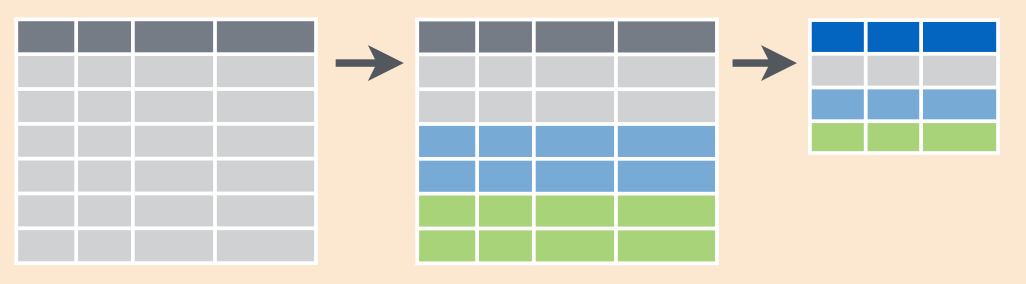
\includegraphics[width=4.16667in]{images/group_by_s.png}
\caption{}
\end{figure}

\subsection{\texorpdfstring{Подсчет строк: \texttt{dplyr::n()},
\texttt{dplyr::count()}}{Подсчет строк: dplyr::n(), dplyr::count()}}\label{tidy_count}

Для подсчет количества значений можно воспользоваться функцией
\texttt{n()}.

\begin{Shaded}
\begin{Highlighting}[]
\NormalTok{heroes }\OperatorTok
\StringTok{  }\KeywordTok{group_by}\NormalTok{(Gender) }\OperatorTok
\StringTok{  }\KeywordTok{summarise}\NormalTok{(}\DataTypeTok{n =} \KeywordTok{n}\NormalTok{())}
\end{Highlighting}
\end{Shaded}

\begin{verbatim}
## `summarise()` ungrouping output (override with `.groups` argument)
\end{verbatim}

\begin{verbatim}
## # A tibble: 3 x 2
##   Gender     n
##   <chr>  <int>
## 1 Female   200
## 2 Male     505
## 3 <NA>      29
\end{verbatim}

Функция \texttt{n()} вместе с \texttt{group\_by()} внутри
\texttt{filter()} позволяет удобным образом ``отрезать'' от тиббла
редкие группы\ldots{}

\begin{Shaded}
\begin{Highlighting}[]
\NormalTok{heroes }\OperatorTok
\StringTok{  }\KeywordTok{group_by}\NormalTok{(Race) }\OperatorTok
\StringTok{  }\KeywordTok{filter}\NormalTok{(}\KeywordTok{n}\NormalTok{() }\OperatorTok{>}\StringTok{ }\DecValTok{10}\NormalTok{) }\OperatorTok
\StringTok{  }\KeywordTok{select}\NormalTok{(name, Race)}
\end{Highlighting}
\end{Shaded}

\begin{verbatim}
## # A tibble: 611 x 2
## # Groups:   Race [6]
##    name          Race             
##    <chr>         <chr>            
##  1 A-Bomb        Human            
##  2 Abomination   Human / Radiation
##  3 Absorbing Man Human            
##  4 Adam Monroe   <NA>             
##  5 Adam Strange  Human            
##  6 Agent 13      <NA>             
##  7 Agent Bob     Human            
##  8 Agent Zero    <NA>             
##  9 Air-Walker    <NA>             
## 10 Ajax          Cyborg           
## # ... with 601 more rows
\end{verbatim}

или же наоборот, выделить только маленькие группы:

\begin{Shaded}
\begin{Highlighting}[]
\NormalTok{heroes }\OperatorTok
\StringTok{  }\KeywordTok{group_by}\NormalTok{(Race) }\OperatorTok
\StringTok{  }\KeywordTok{filter}\NormalTok{(}\KeywordTok{n}\NormalTok{() }\OperatorTok{==}\StringTok{ }\DecValTok{1}\NormalTok{) }\OperatorTok
\StringTok{  }\KeywordTok{select}\NormalTok{(name, Race)}
\end{Highlighting}
\end{Shaded}

\begin{verbatim}
## # A tibble: 34 x 2
## # Groups:   Race [34]
##    name          Race              
##    <chr>         <chr>             
##  1 Abe Sapien    Icthyo Sapien     
##  2 Abin Sur      Ungaran           
##  3 Alien         Xenomorph XX121   
##  4 Azazel        Neyaphem          
##  5 Bizarro       Bizarro           
##  6 Boba Fett     Human / Clone     
##  7 Darth Maul    Dathomirian Zabrak
##  8 Fin Fang Foom Kakarantharaian   
##  9 Gamora        Zen-Whoberian     
## 10 Gladiator     Strontian         
## # ... with 24 more rows
\end{verbatim}

Таблицу частот можно создать без \texttt{group\_by()} и
\texttt{summarise(n\ =\ n())}. Функция \texttt{count()} заменяет эту
конструкцию:

\begin{Shaded}
\begin{Highlighting}[]
\NormalTok{heroes }\OperatorTok
\StringTok{  }\KeywordTok{count}\NormalTok{(Gender)}
\end{Highlighting}
\end{Shaded}

\begin{verbatim}
## # A tibble: 3 x 2
##   Gender     n
##   <chr>  <int>
## 1 Female   200
## 2 Male     505
## 3 <NA>      29
\end{verbatim}

Эту таблицу частот удобно сразу проранжировать, указав в параметре
\texttt{sort\ =} значение \texttt{TRUE}.

\begin{Shaded}
\begin{Highlighting}[]
\NormalTok{heroes }\OperatorTok
\StringTok{  }\KeywordTok{count}\NormalTok{(Gender, }\DataTypeTok{sort =} \OtherTok{TRUE}\NormalTok{)}
\end{Highlighting}
\end{Shaded}

\begin{verbatim}
## # A tibble: 3 x 2
##   Gender     n
##   <chr>  <int>
## 1 Male     505
## 2 Female   200
## 3 <NA>      29
\end{verbatim}

\begin{quote}
Функция \texttt{count()}, несмотря на свою простоту, является одной из
наиболее используемых в tidyverse.
\end{quote}

\subsection{\texorpdfstring{Уникальные значения:
\texttt{dplyr::distinct()}}{Уникальные значения: dplyr::distinct()}}\label{tidy_distinct}

\texttt{dplyr::distinct()} - это более быстрый аналог \texttt{unique()},
позволяет извлекать уникальные значения для одной или нескольких
колонок.

\begin{Shaded}
\begin{Highlighting}[]
\NormalTok{heroes }\OperatorTok
\StringTok{  }\KeywordTok{distinct}\NormalTok{(Gender)}
\end{Highlighting}
\end{Shaded}

\begin{verbatim}
## # A tibble: 3 x 1
##   Gender
##   <chr> 
## 1 Male  
## 2 Female
## 3 <NA>
\end{verbatim}

\begin{Shaded}
\begin{Highlighting}[]
\NormalTok{heroes }\OperatorTok
\StringTok{  }\KeywordTok{distinct}\NormalTok{(Gender, Race)}
\end{Highlighting}
\end{Shaded}

\begin{verbatim}
## # A tibble: 81 x 2
##    Gender Race             
##    <chr>  <chr>            
##  1 Male   Human            
##  2 Male   Icthyo Sapien    
##  3 Male   Ungaran          
##  4 Male   Human / Radiation
##  5 Male   Cosmic Entity    
##  6 Male   <NA>             
##  7 Female <NA>             
##  8 Male   Cyborg           
##  9 Male   Xenomorph XX121  
## 10 Male   Android          
## # ... with 71 more rows
\end{verbatim}

Иногда нужно аггрегировать данные, но при этом сохранить исходную
структуру тиббла. Например, нужно посчитать размер групп или посчитать
средние значения по группе для последующего сравнения с индивидуальными
значениями.

\subsection{Создание колонок с группировкой}\label{tidy_group_mutate}

В tidyverse это можно сделать с помощью сочетания \texttt{group\_by()} и
\texttt{mutate()} (вместо \texttt{summarise()}):

\begin{Shaded}
\begin{Highlighting}[]
\NormalTok{heroes }\OperatorTok
\StringTok{  }\KeywordTok{group_by}\NormalTok{(Race) }\OperatorTok
\StringTok{  }\KeywordTok{mutate}\NormalTok{(}\DataTypeTok{Race_n =} \KeywordTok{n}\NormalTok{()) }\OperatorTok
\StringTok{  }\KeywordTok{select}\NormalTok{(Race, name, Gender, Race_n)}
\end{Highlighting}
\end{Shaded}

\begin{verbatim}
## # A tibble: 734 x 4
## # Groups:   Race [62]
##    Race              name          Gender Race_n
##    <chr>             <chr>         <chr>   <int>
##  1 Human             A-Bomb        Male      208
##  2 Icthyo Sapien     Abe Sapien    Male        1
##  3 Ungaran           Abin Sur      Male        1
##  4 Human / Radiation Abomination   Male       11
##  5 Cosmic Entity     Abraxas       Male        4
##  6 Human             Absorbing Man Male      208
##  7 <NA>              Adam Monroe   Male      304
##  8 Human             Adam Strange  Male      208
##  9 <NA>              Agent 13      Female    304
## 10 Human             Agent Bob     Male      208
## # ... with 724 more rows
\end{verbatim}

Результаты аггрегации были записаны в отдельную колонку, при этом
значения этой колонки внутри одной группы повторяются:

\begin{figure}
\centering
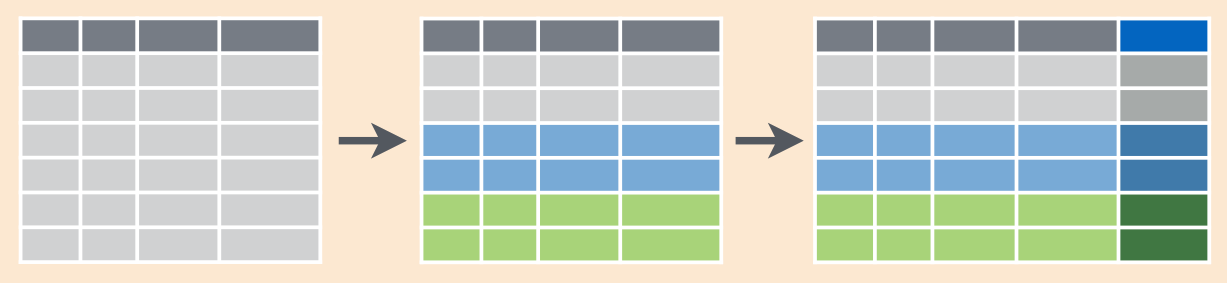
\includegraphics[width=4.16667in]{images/group_by_m.png}
\caption{}
\end{figure}

\chapter{Продвинутый tidyverse}\label{tidyverse_advanced}

\section{\texorpdfstring{Трансформация нескольких колонок:
\texttt{dplyr::across()}}{Трансформация нескольких колонок: dplyr::across()}}\label{ux442ux440ux430ux43dux441ux444ux43eux440ux43cux430ux446ux438ux44f-ux43dux435ux441ux43aux43eux43bux44cux43aux438ux445-ux43aux43eux43bux43eux43dux43eux43a-dplyracross}

Допустим, вы хотите посчитать среднюю массу и рост, группируя по полу
супергероев. Можно посчитать это внутри одного \texttt{summarise()},
использую запятую:

\begin{Shaded}
\begin{Highlighting}[]
\NormalTok{heroes }\OperatorTok
\StringTok{  }\KeywordTok{group_by}\NormalTok{(Gender) }\OperatorTok
\StringTok{  }\KeywordTok{summarise}\NormalTok{(}\DataTypeTok{height =} \KeywordTok{mean}\NormalTok{(Height, }\DataTypeTok{na.rm =} \OtherTok{TRUE}\NormalTok{),}
            \DataTypeTok{weight =} \KeywordTok{mean}\NormalTok{(Weight, }\DataTypeTok{na.rm =} \OtherTok{TRUE}\NormalTok{))}
\end{Highlighting}
\end{Shaded}

\begin{verbatim}
## `summarise()` ungrouping output (override with `.groups` argument)
\end{verbatim}

\begin{verbatim}
## # A tibble: 3 x 3
##   Gender height weight
##   <chr>   <dbl>  <dbl>
## 1 Female   175.   78.8
## 2 Male     192.  126. 
## 3 <NA>     177.  129.
\end{verbatim}

Если таких колонок будет много, то это уже станет сильно неудобным, нам
придется много копировать код, а это чревато ошибками и очень скучно.

Поэтому в \texttt{dplyr} есть функция для операций над несколькими
колонками сразу: \texttt{dplyr::across()}\footnote{Функция
  \texttt{across()} появилась в пакете \texttt{dplyr} относительно
  недавно, до этого для работы с множественными колонками в tidyverse
  использовались многочисленные функции \texttt{*\_at()},
  \texttt{*\_if()}, \texttt{*\_all()}, например,
  \texttt{summarise\_at()}, \texttt{summarise\_if()},
  \texttt{summarize\_all()}. Эти функции до сих пор присутствуют в
  \texttt{dplyr}, но считаются устаревшими. Другая альтернатива -
  использование пакета \texttt{purrr} (\ref{purrr}) или семейства
  функций \texttt{apply()} (@ref(apply\_f)).}. Эта функция работает
похожим образом на функции семейства \texttt{apply()} и использует
tidyselect для выбора колонок.

Таким образом, конструкции с функцией \texttt{across()} можно разбить на
три части:

\begin{enumerate}
\def\labelenumi{\arabic{enumi}.}
\tightlist
\item
  Выбор колонок с помощью tidyselect. Здесь работают все те приемы,
  которые мы изучили при выборе колонок (\ref{tidyselect}).
\item
  Собственно применение функции \texttt{across()}. Первый аргумент
  \texttt{.col} --- колонки, выбранные на первом этапе с помощью
  tidyselect, по умолчанию это \texttt{everything()}, т.е. все колонки.
  Второй аргумент \texttt{.fns} --- это функция или целый список из
  функций, которые будут применены к выбранным колонкам. Если функции
  требуют дополнительных аргументов, то они могут быть перечислены
  внутри \texttt{across()}.
\item
  Использование \texttt{summarise()} или другой функции \texttt{dplyr}.
  В этом случае в качестве аргумента для функции используется результат
  работы функции \texttt{across()}.
\end{enumerate}

Вот такой вот бутерброд выходит. Давайте посмотрим, как это работает на
практике и посчитаем среднее значение по колонкам \texttt{Height} и
\texttt{Weight}.

\begin{Shaded}
\begin{Highlighting}[]
\NormalTok{heroes }\OperatorTok
\StringTok{  }\KeywordTok{group_by}\NormalTok{(Gender) }\OperatorTok
\StringTok{  }\KeywordTok{summarise}\NormalTok{(}\KeywordTok{across}\NormalTok{(}\KeywordTok{c}\NormalTok{(Height,Weight), mean))}
\end{Highlighting}
\end{Shaded}

\begin{verbatim}
## `summarise()` ungrouping output (override with `.groups` argument)
\end{verbatim}

\begin{verbatim}
## # A tibble: 3 x 3
##   Gender Height Weight
##   <chr>   <dbl>  <dbl>
## 1 Female     NA     NA
## 2 Male       NA     NA
## 3 <NA>       NA     NA
\end{verbatim}

Здесь мы столкнулись с уже известной нам проблемой: функция
\texttt{mean()} при столкновении хотя бы с одним \texttt{NA} будет
возвращать \texttt{NA}, если мы не изменим параметр \texttt{na.rm\ =}.
Как и в случае с функциями семейства \texttt{apply()} (@ref(apply\_f)),
дополнительные параметры для функции можно перечислить через запятую
после самой функции:

\begin{Shaded}
\begin{Highlighting}[]
\NormalTok{heroes }\OperatorTok
\StringTok{  }\KeywordTok{group_by}\NormalTok{(Gender) }\OperatorTok
\StringTok{  }\KeywordTok{summarise}\NormalTok{(}\KeywordTok{across}\NormalTok{(}\KeywordTok{c}\NormalTok{(Height, Weight), mean, }\DataTypeTok{na.rm =} \OtherTok{TRUE}\NormalTok{))}
\end{Highlighting}
\end{Shaded}

\begin{verbatim}
## `summarise()` ungrouping output (override with `.groups` argument)
\end{verbatim}

\begin{verbatim}
## # A tibble: 3 x 3
##   Gender Height Weight
##   <chr>   <dbl>  <dbl>
## 1 Female   175.   78.8
## 2 Male     192.  126. 
## 3 <NA>     177.  129.
\end{verbatim}

До этого мы просто использовали выбор колонок по их названию. Но именно
внутри \texttt{across()} использование tidyselect раскрывается как
удивительно элегантный и мощный инструмент. Например, можно посчитать
среднее для всех numeric колонок:

\begin{Shaded}
\begin{Highlighting}[]
\NormalTok{heroes }\OperatorTok
\StringTok{  }\KeywordTok{drop_na}\NormalTok{(Height, Weight) }\OperatorTok
\StringTok{  }\KeywordTok{group_by}\NormalTok{(Gender) }\OperatorTok
\StringTok{  }\KeywordTok{summarise}\NormalTok{(}\KeywordTok{across}\NormalTok{(}\KeywordTok{where}\NormalTok{(is.numeric), mean, }\DataTypeTok{na.rm =} \OtherTok{TRUE}\NormalTok{))}
\end{Highlighting}
\end{Shaded}

\begin{verbatim}
## `summarise()` ungrouping output (override with `.groups` argument)
\end{verbatim}

\begin{verbatim}
## # A tibble: 3 x 4
##   Gender    X1 Height Weight
##   <chr>  <dbl>  <dbl>  <dbl>
## 1 Female  394.   174.   78.3
## 2 Male    369.   193.  126. 
## 3 <NA>    375.   182   129.
\end{verbatim}

Или длину строк для строковых колонок. Для этого нам понадобится
вспомнить, как создавать анонимные функции (@ref(anon\_f)).

\begin{Shaded}
\begin{Highlighting}[]
\NormalTok{heroes }\OperatorTok
\StringTok{  }\KeywordTok{group_by}\NormalTok{(Gender) }\OperatorTok
\StringTok{  }\KeywordTok{summarise}\NormalTok{(}\KeywordTok{across}\NormalTok{(}\KeywordTok{where}\NormalTok{(is.character), }
                   \ControlFlowTok{function}\NormalTok{(x) }\KeywordTok{mean}\NormalTok{(}\KeywordTok{nchar}\NormalTok{(x), }\DataTypeTok{na.rm =} \OtherTok{TRUE}\NormalTok{)))}
\end{Highlighting}
\end{Shaded}

\begin{verbatim}
## `summarise()` ungrouping output (override with `.groups` argument)
\end{verbatim}

\begin{verbatim}
## # A tibble: 3 x 8
##   Gender  name `Eye color`  Race `Hair color` Publisher `Skin color` Alignment
##   <chr>  <dbl>       <dbl> <dbl>        <dbl>     <dbl>        <dbl>     <dbl>
## 1 Female  9.04        4.68  6.42         5.05      11.5         4.57      3.88
## 2 Male    9.05        4.53  6.75         5.48      11.4         5.02      3.78
## 3 <NA>    9.48        5.16 10.1          6.44      11.9         4         3.96
\end{verbatim}

Или же даже посчитать и то, и другое внутри одного \texttt{summarise()}!

\begin{Shaded}
\begin{Highlighting}[]
\NormalTok{heroes }\OperatorTok
\StringTok{  }\KeywordTok{group_by}\NormalTok{(Gender) }\OperatorTok
\StringTok{  }\KeywordTok{summarise}\NormalTok{(}\KeywordTok{across}\NormalTok{(}\KeywordTok{where}\NormalTok{(is.numeric), mean, }\DataTypeTok{na.rm =} \OtherTok{TRUE}\NormalTok{),}
            \KeywordTok{across}\NormalTok{(}\KeywordTok{where}\NormalTok{(is.character), }
                   \ControlFlowTok{function}\NormalTok{(x) }\KeywordTok{mean}\NormalTok{(}\KeywordTok{nchar}\NormalTok{(x), }\DataTypeTok{na.rm =} \OtherTok{TRUE}\NormalTok{)))}
\end{Highlighting}
\end{Shaded}

\begin{verbatim}
## `summarise()` ungrouping output (override with `.groups` argument)
\end{verbatim}

\begin{verbatim}
## # A tibble: 3 x 11
##   Gender    X1 Height Weight  name `Eye color`  Race `Hair color` Publisher
##   <chr>  <dbl>  <dbl>  <dbl> <dbl>       <dbl> <dbl>        <dbl>     <dbl>
## 1 Female  395.   175.   78.8  9.04        4.68  6.42         5.05      11.5
## 2 Male    357.   192.  126.   9.05        4.53  6.75         5.48      11.4
## 3 <NA>    329    177.  129.   9.48        5.16 10.1          6.44      11.9
## # ... with 2 more variables: `Skin color` <dbl>, Alignment <dbl>
\end{verbatim}

Внутри одного \texttt{across()} можно применить не одну функцию к каждой
из выбранных колонок, а сразу несколько функций для каждой из колонок.
Для этого нам нужно использовать список функций (желательно -
проименованный).

\begin{Shaded}
\begin{Highlighting}[]
\NormalTok{heroes }\OperatorTok
\StringTok{  }\KeywordTok{group_by}\NormalTok{(Gender) }\OperatorTok
\StringTok{  }\KeywordTok{summarise}\NormalTok{(}\KeywordTok{across}\NormalTok{(}\KeywordTok{c}\NormalTok{(Height, Weight), }
                   \KeywordTok{list}\NormalTok{(}\DataTypeTok{minimum =}\NormalTok{ min,}
                        \DataTypeTok{average =}\NormalTok{ mean,}
                        \DataTypeTok{maximum =}\NormalTok{ max), }
                   \DataTypeTok{na.rm =} \OtherTok{TRUE}\NormalTok{))}
\end{Highlighting}
\end{Shaded}

\begin{verbatim}
## `summarise()` ungrouping output (override with `.groups` argument)
\end{verbatim}

\begin{verbatim}
## # A tibble: 3 x 7
##   Gender Height_minimum Height_average Height_maximum Weight_minimum
##   <chr>           <dbl>          <dbl>          <dbl>          <dbl>
## 1 Female           62.5           175.            366             41
## 2 Male             15.2           192.            975              2
## 3 <NA>            108             177.            198             39
## # ... with 2 more variables: Weight_average <dbl>, Weight_maximum <dbl>
\end{verbatim}

\begin{quote}
Вот нам и понадобился список функций (@ref(functions\_objects))!
\end{quote}

\begin{Shaded}
\begin{Highlighting}[]
\NormalTok{heroes }\OperatorTok
\StringTok{  }\KeywordTok{group_by}\NormalTok{(Gender) }\OperatorTok
\StringTok{  }\KeywordTok{summarise}\NormalTok{(}\KeywordTok{across}\NormalTok{(}\KeywordTok{c}\NormalTok{(Height, Weight),}
                   \KeywordTok{list}\NormalTok{(}\DataTypeTok{min =} \ControlFlowTok{function}\NormalTok{(x) }\KeywordTok{min}\NormalTok{(x, }\DataTypeTok{na.rm =} \OtherTok{TRUE}\NormalTok{),}
                        \DataTypeTok{mean =} \ControlFlowTok{function}\NormalTok{(x) }\KeywordTok{mean}\NormalTok{(x, }\DataTypeTok{na.rm =} \OtherTok{TRUE}\NormalTok{),}
                        \DataTypeTok{max =} \ControlFlowTok{function}\NormalTok{(x) }\KeywordTok{max}\NormalTok{(x, }\DataTypeTok{na.rm =} \OtherTok{TRUE}\NormalTok{),}
                        \DataTypeTok{na_n =} \ControlFlowTok{function}\NormalTok{(x, ...) }\KeywordTok{sum}\NormalTok{(}\KeywordTok{is.na}\NormalTok{(x)))}
\NormalTok{                   )}
\NormalTok{            )}
\end{Highlighting}
\end{Shaded}

\begin{verbatim}
## `summarise()` ungrouping output (override with `.groups` argument)
\end{verbatim}

\begin{verbatim}
## # A tibble: 3 x 9
##   Gender Height_min Height_mean Height_max Height_na_n Weight_min Weight_mean
##   <chr>       <dbl>       <dbl>      <dbl>       <int>      <dbl>       <dbl>
## 1 Female       62.5        175.        366          56         41        78.8
## 2 Male         15.2        192.        975         147          2       126. 
## 3 <NA>        108          177.        198          14         39       129. 
## # ... with 2 more variables: Weight_max <dbl>, Weight_na_n <int>
\end{verbatim}

Хотя основное применение функции \texttt{across()} --- это массовое
подытоживание с помощью \texttt{summarise()}, \texttt{across()} можно
использовать и с другими функциями \texttt{dplyr}. Например, можно
делать массовые операции с колонками с помощью \texttt{mutate()}:

\begin{Shaded}
\begin{Highlighting}[]
\NormalTok{heroes }\OperatorTok
\StringTok{  }\KeywordTok{mutate}\NormalTok{(}\KeywordTok{across}\NormalTok{(}\KeywordTok{where}\NormalTok{(is.character), as.factor))}
\end{Highlighting}
\end{Shaded}

\begin{verbatim}
## # A tibble: 734 x 11
##       X1 name  Gender `Eye color` Race  `Hair color` Height Publisher
##    <dbl> <fct> <fct>  <fct>       <fct> <fct>         <dbl> <fct>    
##  1     0 A-Bo~ Male   yellow      Human No Hair         203 Marvel C~
##  2     1 Abe ~ Male   blue        Icth~ No Hair         191 Dark Hor~
##  3     2 Abin~ Male   blue        Unga~ No Hair         185 DC Comics
##  4     3 Abom~ Male   green       Huma~ No Hair         203 Marvel C~
##  5     4 Abra~ Male   blue        Cosm~ Black            NA Marvel C~
##  6     5 Abso~ Male   blue        Human No Hair         193 Marvel C~
##  7     6 Adam~ Male   blue        <NA>  Blond            NA NBC - He~
##  8     7 Adam~ Male   blue        Human Blond           185 DC Comics
##  9     8 Agen~ Female blue        <NA>  Blond           173 Marvel C~
## 10     9 Agen~ Male   brown       Human Brown           178 Marvel C~
## # ... with 724 more rows, and 3 more variables: `Skin color` <fct>,
## #   Alignment <fct>, Weight <dbl>
\end{verbatim}

Менее очевидный способ применения \texttt{across()} - использование
\texttt{across()} внутри \texttt{count()} вместе с функцией
\texttt{n\_distinct()}, которая считает количество уникальных значений в
векторе. Это позволяет посмотреть таблицу частот для группирующих
переменных:

\begin{Shaded}
\begin{Highlighting}[]
\NormalTok{heroes }\OperatorTok
\StringTok{  }\KeywordTok{select}\NormalTok{(}\KeywordTok{where}\NormalTok{(}\ControlFlowTok{function}\NormalTok{(x) }\KeywordTok{n_distinct}\NormalTok{(x) }\OperatorTok{<=}\StringTok{ }\DecValTok{6}\NormalTok{))}
\end{Highlighting}
\end{Shaded}

\begin{verbatim}
## # A tibble: 734 x 2
##    Gender Alignment
##    <chr>  <chr>    
##  1 Male   good     
##  2 Male   good     
##  3 Male   good     
##  4 Male   bad      
##  5 Male   bad      
##  6 Male   bad      
##  7 Male   good     
##  8 Male   good     
##  9 Female good     
## 10 Male   good     
## # ... with 724 more rows
\end{verbatim}

\begin{Shaded}
\begin{Highlighting}[]
\NormalTok{heroes }\OperatorTok
\StringTok{  }\KeywordTok{count}\NormalTok{(}\KeywordTok{across}\NormalTok{(}\KeywordTok{where}\NormalTok{(}\ControlFlowTok{function}\NormalTok{(x) }\KeywordTok{n_distinct}\NormalTok{(x) }\OperatorTok{<=}\StringTok{ }\DecValTok{6}\NormalTok{)))}
\end{Highlighting}
\end{Shaded}

\begin{verbatim}
## # A tibble: 11 x 3
##    Gender Alignment     n
##    <chr>  <chr>     <int>
##  1 Female bad          35
##  2 Female good        161
##  3 Female neutral       4
##  4 Male   bad         165
##  5 Male   good        316
##  6 Male   neutral      18
##  7 Male   <NA>          6
##  8 <NA>   bad           7
##  9 <NA>   good         19
## 10 <NA>   neutral       2
## 11 <NA>   <NA>          1
\end{verbatim}

\section{Объединение нескольких датафреймов}\label{tidy_several}

\subsection{Соединение структурно схожих датафреймов: bind\_rows(),
bind\_cols()}\label{tidy_bind}

Для начала создадим следующие тибблы и сохраним их как \texttt{dc},
\texttt{marvel} и \texttt{other\_publishers}:

\begin{Shaded}
\begin{Highlighting}[]
\NormalTok{dc <-}\StringTok{ }\NormalTok{heroes }\OperatorTok
\StringTok{  }\KeywordTok{filter}\NormalTok{(Publisher }\OperatorTok{==}\StringTok{ "DC Comics"}\NormalTok{) }\OperatorTok
\StringTok{  }\KeywordTok{group_by}\NormalTok{(Gender) }\OperatorTok
\StringTok{  }\KeywordTok{summarise}\NormalTok{(}\DataTypeTok{weight_mean =} \KeywordTok{mean}\NormalTok{(Weight, }\DataTypeTok{na.rm =} \OtherTok{TRUE}\NormalTok{))}
\end{Highlighting}
\end{Shaded}

\begin{verbatim}
## `summarise()` ungrouping output (override with `.groups` argument)
\end{verbatim}

\begin{Shaded}
\begin{Highlighting}[]
\NormalTok{dc}
\end{Highlighting}
\end{Shaded}

\begin{verbatim}
## # A tibble: 3 x 2
##   Gender weight_mean
##   <chr>        <dbl>
## 1 Female        76.8
## 2 Male         113. 
## 3 <NA>         NaN
\end{verbatim}

\begin{Shaded}
\begin{Highlighting}[]
\NormalTok{marvel <-}\StringTok{ }\NormalTok{heroes }\OperatorTok
\StringTok{  }\KeywordTok{filter}\NormalTok{(Publisher }\OperatorTok{==}\StringTok{ "Marvel Comics"}\NormalTok{) }\OperatorTok
\StringTok{  }\KeywordTok{group_by}\NormalTok{(Gender) }\OperatorTok
\StringTok{  }\KeywordTok{summarise}\NormalTok{(}\DataTypeTok{weight_mean =} \KeywordTok{mean}\NormalTok{(Weight, }\DataTypeTok{na.rm =} \OtherTok{TRUE}\NormalTok{))}
\end{Highlighting}
\end{Shaded}

\begin{verbatim}
## `summarise()` ungrouping output (override with `.groups` argument)
\end{verbatim}

\begin{Shaded}
\begin{Highlighting}[]
\NormalTok{marvel}
\end{Highlighting}
\end{Shaded}

\begin{verbatim}
## # A tibble: 3 x 2
##   Gender weight_mean
##   <chr>        <dbl>
## 1 Female        80.1
## 2 Male         134. 
## 3 <NA>         129.
\end{verbatim}

\begin{Shaded}
\begin{Highlighting}[]
\NormalTok{other_publishers <-}\StringTok{ }\NormalTok{heroes }\OperatorTok
\StringTok{  }\KeywordTok{filter}\NormalTok{(}\OperatorTok{!}\NormalTok{(Publisher }\OperatorTok\StringTok{ }\KeywordTok{c}\NormalTok{(}\StringTok{"DC Comics"}\NormalTok{,}\StringTok{"Marvel Comics"}\NormalTok{))) }\OperatorTok
\StringTok{  }\KeywordTok{group_by}\NormalTok{(Gender) }\OperatorTok
\StringTok{  }\KeywordTok{summarise}\NormalTok{(}\DataTypeTok{weight_mean =} \KeywordTok{mean}\NormalTok{(Weight, }\DataTypeTok{na.rm =} \OtherTok{TRUE}\NormalTok{))}
\end{Highlighting}
\end{Shaded}

\begin{verbatim}
## `summarise()` ungrouping output (override with `.groups` argument)
\end{verbatim}

\begin{Shaded}
\begin{Highlighting}[]
\NormalTok{other_publishers}
\end{Highlighting}
\end{Shaded}

\begin{verbatim}
## # A tibble: 3 x 2
##   Gender weight_mean
##   <chr>        <dbl>
## 1 Female        70.8
## 2 Male         111. 
## 3 <NA>         NaN
\end{verbatim}

Несколько тибблов можно объединить вертикально с помощью функции
\texttt{bind\_rows()}. Для корректного объединения тибблы должны иметь
одинаковые названия колонок.

\begin{Shaded}
\begin{Highlighting}[]
\KeywordTok{bind_rows}\NormalTok{(dc, marvel)}
\end{Highlighting}
\end{Shaded}

\begin{verbatim}
## # A tibble: 6 x 2
##   Gender weight_mean
##   <chr>        <dbl>
## 1 Female        76.8
## 2 Male         113. 
## 3 <NA>         NaN  
## 4 Female        80.1
## 5 Male         134. 
## 6 <NA>         129.
\end{verbatim}

Чтобы соединить тибблы горизонтально, воспользуйтесь функцией
\texttt{bind\_cols()}.

\begin{Shaded}
\begin{Highlighting}[]
\KeywordTok{bind_cols}\NormalTok{(dc, marvel)}
\end{Highlighting}
\end{Shaded}

\begin{verbatim}
## New names:
## * Gender -> Gender...1
## * weight_mean -> weight_mean...2
## * Gender -> Gender...3
## * weight_mean -> weight_mean...4
\end{verbatim}

\begin{verbatim}
## # A tibble: 3 x 4
##   Gender...1 weight_mean...2 Gender...3 weight_mean...4
##   <chr>                <dbl> <chr>                <dbl>
## 1 Female                76.8 Female                80.1
## 2 Male                 113.  Male                 134. 
## 3 <NA>                 NaN   <NA>                 129.
\end{verbatim}

Функции \texttt{bind\_rows()} и \texttt{bind\_cols()} могут работать не
только с двумя, но сразу с несколькими датафреймами.

\begin{Shaded}
\begin{Highlighting}[]
\KeywordTok{bind_rows}\NormalTok{(dc, marvel, other_publishers)}
\end{Highlighting}
\end{Shaded}

\begin{verbatim}
## # A tibble: 9 x 2
##   Gender weight_mean
##   <chr>        <dbl>
## 1 Female        76.8
## 2 Male         113. 
## 3 <NA>         NaN  
## 4 Female        80.1
## 5 Male         134. 
## 6 <NA>         129. 
## 7 Female        70.8
## 8 Male         111. 
## 9 <NA>         NaN
\end{verbatim}

На входе в функции \texttt{bind\_rows()} и \texttt{bind\_cold()} можно
подавать как сами датафреймы или тибблы через запятую, так и список из
датафреймов/тибблов.

\begin{Shaded}
\begin{Highlighting}[]
\NormalTok{heroes_list_of_df <-}\StringTok{ }\KeywordTok{list}\NormalTok{(}\DataTypeTok{DC =}\NormalTok{ dc, }
                          \DataTypeTok{Marvel =}\NormalTok{ marvel, }
                          \DataTypeTok{Other =}\NormalTok{ other_publishers)}
\KeywordTok{bind_rows}\NormalTok{(heroes_list_of_df)}
\end{Highlighting}
\end{Shaded}

\begin{verbatim}
## # A tibble: 9 x 2
##   Gender weight_mean
##   <chr>        <dbl>
## 1 Female        76.8
## 2 Male         113. 
## 3 <NA>         NaN  
## 4 Female        80.1
## 5 Male         134. 
## 6 <NA>         129. 
## 7 Female        70.8
## 8 Male         111. 
## 9 <NA>         NaN
\end{verbatim}

Чтобы не потерять, из какого датафрейма какие данные, можно указать
любое строковое значение (название будущей колонки) для необязательного
аргумента \texttt{.id\ =}.

\begin{Shaded}
\begin{Highlighting}[]
\KeywordTok{bind_rows}\NormalTok{(heroes_list_of_df, }\DataTypeTok{.id =} \StringTok{"Publisher"}\NormalTok{)}
\end{Highlighting}
\end{Shaded}

\begin{verbatim}
## # A tibble: 9 x 3
##   Publisher Gender weight_mean
##   <chr>     <chr>        <dbl>
## 1 DC        Female        76.8
## 2 DC        Male         113. 
## 3 DC        <NA>         NaN  
## 4 Marvel    Female        80.1
## 5 Marvel    Male         134. 
## 6 Marvel    <NA>         129. 
## 7 Other     Female        70.8
## 8 Other     Male         111. 
## 9 Other     <NA>         NaN
\end{verbatim}

\texttt{bind\_rows()} обычно используется, когда ваши данные находятся в
разных файлах с одинаковой структурой. Тогда вы можете прочитать все
таблицы в папке, сохранить их в качестве списка из датафреймов и
объединить в один датафрейм с помощью \texttt{bind\_rows()}.

\subsection{\texorpdfstring{Реляционные данные:
\texttt{*\_join()}}{Реляционные данные: *\_join()}}\label{tidy_join}

В реальности иногда возникает ситуация, когда нужно соединить две
таблички, у которых есть общий столбец (или несколько столбцов), но все
остальные столбцы различаются. Табличек может быть и больше, это может
быть целая сеть таблиц, некоторые из которых содержат основные данные, а
некоторые - дополнительные, которые необходимо на определенном этапе
``включить'' в анализ. Например, таблица с расшифровкой аббревиатур или
сокращений вроде коротких названий стран или таблица телефонных кодов
разных стран. Совокупность нескольких связанных друг с другом таблиц
называют реляционными данными.

В случае с реляционными данными простых \texttt{bind\_rows()} и
\texttt{bind\_cols()} становится недостаточно.

Эти две таблички нужно объединить (\emph{join}). Эта задача обычно
возникает не очень часто, обычно это происходит один-два раза в одном
проекте, когда нужно дополнить имеющиеся данные дополнительной
информацией извне или объединить два набора данных, обрабатывавшихся в
разных программах. Всякий раз, когда такая задача возникает, это
доставляет много боли. \texttt{dplyr} предлагает интуитивно понятный
инструмент для объединения реляционных данных - семейство функций
\texttt{*\_join()}.

Возьмем для примера два тиббла \texttt{band\_members} и
\texttt{band\_instruments}, встроенных в \texttt{dplyr} специально для
демонстрации работы функций \texttt{*\_join()}.

\begin{Shaded}
\begin{Highlighting}[]
\NormalTok{band_members}
\end{Highlighting}
\end{Shaded}

\begin{verbatim}
## # A tibble: 3 x 2
##   name  band   
##   <chr> <chr>  
## 1 Mick  Stones 
## 2 John  Beatles
## 3 Paul  Beatles
\end{verbatim}

\begin{Shaded}
\begin{Highlighting}[]
\NormalTok{band_instruments}
\end{Highlighting}
\end{Shaded}

\begin{verbatim}
## # A tibble: 3 x 2
##   name  plays 
##   <chr> <chr> 
## 1 John  guitar
## 2 Paul  bass  
## 3 Keith guitar
\end{verbatim}

У этих двух тибблов есть колонка с одинаковым названием, которая по
своему смыслу соединяет данные обоих тибблов. Такая колонка называется
\textbf{ключом}. Ключ должен однозначно идентифицировать
наблюдения\footnote{Если ключи будут неуникальными, то функции
  \texttt{*\_join()} не будут выдавать ошибку. Вместо этого они добавят
  в итоговую таблицу все возможные пересечения повторяющихся ключей. С
  этим нужно быть очень осторожным, поэтому рекомендуется, во-первых,
  проверять уникальность ключей на входе и, во-вторых, проверять тиббл
  на выходе. Ну или использовать эту особенность работы функции
  \texttt{*\_join()} себе во благо.}.

Давайте попробуем посоединять \texttt{band\_members} и
\texttt{band\_instruments} разными вариантами \texttt{*\_join()} и
посмотрим, что у нас получится. Все эти функции имеют на входе два
обязательных аргумента (\texttt{x\ =} и \texttt{y\ =}) в которые мы
должны подставить два датафрейма/тиббла которые мы хотим объединить.
Главное различие между этими функциями заключается в том, что они будут
делать, если уникальные значения в ключах \texttt{x} и \texttt{y} не
соответствуют друг другу.

\begin{figure}
\centering
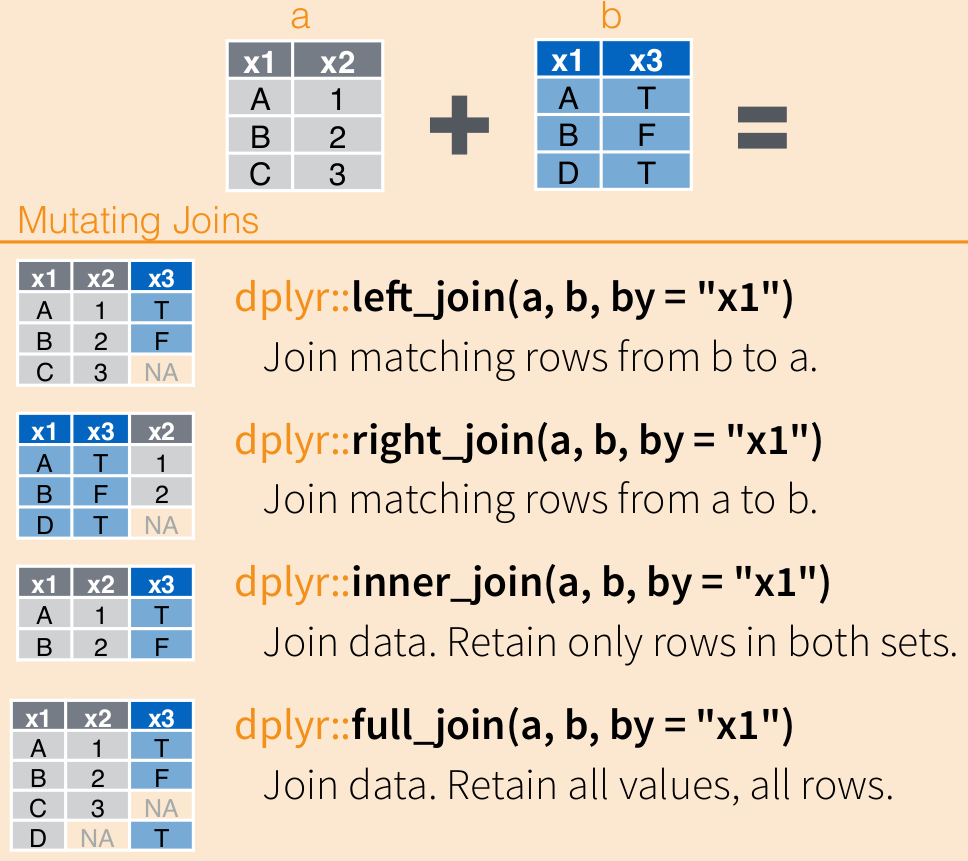
\includegraphics[width=4.16667in]{images/joins.png}
\caption{}
\end{figure}

\begin{itemize}
\tightlist
\item
  \texttt{left\_join()}:
\end{itemize}

\begin{Shaded}
\begin{Highlighting}[]
\NormalTok{band_members }\OperatorTok
\StringTok{  }\KeywordTok{left_join}\NormalTok{(band_instruments)}
\end{Highlighting}
\end{Shaded}

\begin{verbatim}
## Joining, by = "name"
\end{verbatim}

\begin{verbatim}
## # A tibble: 3 x 3
##   name  band    plays 
##   <chr> <chr>   <chr> 
## 1 Mick  Stones  <NA>  
## 2 John  Beatles guitar
## 3 Paul  Beatles bass
\end{verbatim}

\texttt{left\_join()} - это самая простая для понимания и самая
используемая функция из семейства \texttt{*\_join()}. Она как бы
``дополняет'' информацию из первого тиббла вторым тибблом. В этом случае
сохраняются все уникальные наблюдения в \texttt{x}, но отбрасываются
лишние наблюдения в тиббле \texttt{y}. Тем значениям, которым не нашлось
соотвествия в \texttt{y}, в колонках, взятых их \texttt{y}, ставятся
значения \texttt{NA}.

Вы можете сами задать колонки-ключи параметром \texttt{by\ =}, по
умолчанию это все колонки с одинаковыми названиями в двух тибблах.

\begin{Shaded}
\begin{Highlighting}[]
\NormalTok{band_members }\OperatorTok
\StringTok{  }\KeywordTok{left_join}\NormalTok{(band_instruments, }\DataTypeTok{by =} \StringTok{"name"}\NormalTok{)}
\end{Highlighting}
\end{Shaded}

\begin{verbatim}
## # A tibble: 3 x 3
##   name  band    plays 
##   <chr> <chr>   <chr> 
## 1 Mick  Stones  <NA>  
## 2 John  Beatles guitar
## 3 Paul  Beatles bass
\end{verbatim}

Часто случается, что колонки-ключи называются по-разному в двух тибблах.
Их необязательно переименовывать, можно поставить соответстие вручную
используя проименованный вектор:

\begin{Shaded}
\begin{Highlighting}[]
\NormalTok{band_members }\OperatorTok
\StringTok{  }\KeywordTok{left_join}\NormalTok{(band_instruments2, }\DataTypeTok{by =} \KeywordTok{c}\NormalTok{(}\StringTok{"name"}\NormalTok{ =}\StringTok{ "artist"}\NormalTok{))}
\end{Highlighting}
\end{Shaded}

\begin{verbatim}
## # A tibble: 3 x 3
##   name  band    plays 
##   <chr> <chr>   <chr> 
## 1 Mick  Stones  <NA>  
## 2 John  Beatles guitar
## 3 Paul  Beatles bass
\end{verbatim}

\begin{itemize}
\tightlist
\item
  \texttt{right\_join()}:
\end{itemize}

\begin{Shaded}
\begin{Highlighting}[]
\NormalTok{band_members }\OperatorTok
\StringTok{  }\KeywordTok{right_join}\NormalTok{(band_instruments)}
\end{Highlighting}
\end{Shaded}

\begin{verbatim}
## Joining, by = "name"
\end{verbatim}

\begin{verbatim}
## # A tibble: 3 x 3
##   name  band    plays 
##   <chr> <chr>   <chr> 
## 1 John  Beatles guitar
## 2 Paul  Beatles bass  
## 3 Keith <NA>    guitar
\end{verbatim}

\texttt{right\_join()} отбрасывает строчки в \texttt{x}, которых не было
в \texttt{y}, но сохраняет соответствующие строчки \texttt{y} -
\texttt{left\_join()} наоборот.

\begin{itemize}
\tightlist
\item
  \texttt{full\_join()}:
\end{itemize}

\begin{Shaded}
\begin{Highlighting}[]
\NormalTok{band_members }\OperatorTok
\StringTok{  }\KeywordTok{full_join}\NormalTok{(band_instruments)}
\end{Highlighting}
\end{Shaded}

\begin{verbatim}
## Joining, by = "name"
\end{verbatim}

\begin{verbatim}
## # A tibble: 4 x 3
##   name  band    plays 
##   <chr> <chr>   <chr> 
## 1 Mick  Stones  <NA>  
## 2 John  Beatles guitar
## 3 Paul  Beatles bass  
## 4 Keith <NA>    guitar
\end{verbatim}

Функция \texttt{full\_join()} сохраняет все строчки и из \texttt{x} и
\texttt{y}. Пожалуй, наиболее используемая функция после
\texttt{left\_join()} --- благодаря \texttt{full\_join()} вы точно
ничего не потеряете при объединении.

\begin{itemize}
\tightlist
\item
  \texttt{inner\_join()}:
\end{itemize}

\begin{Shaded}
\begin{Highlighting}[]
\NormalTok{band_members }\OperatorTok
\StringTok{  }\KeywordTok{inner_join}\NormalTok{(band_instruments)}
\end{Highlighting}
\end{Shaded}

\begin{verbatim}
## Joining, by = "name"
\end{verbatim}

\begin{verbatim}
## # A tibble: 2 x 3
##   name  band    plays 
##   <chr> <chr>   <chr> 
## 1 John  Beatles guitar
## 2 Paul  Beatles bass
\end{verbatim}

Функция \texttt{full\_join()} сохраняет только строчки, которые
присутствуют и в \texttt{x}, и в \texttt{y}.

\begin{itemize}
\tightlist
\item
  \texttt{semi\_join()}:
\end{itemize}

\begin{Shaded}
\begin{Highlighting}[]
\NormalTok{band_members }\OperatorTok
\StringTok{  }\KeywordTok{semi_join}\NormalTok{(band_instruments)}
\end{Highlighting}
\end{Shaded}

\begin{verbatim}
## Joining, by = "name"
\end{verbatim}

\begin{verbatim}
## # A tibble: 2 x 2
##   name  band   
##   <chr> <chr>  
## 1 John  Beatles
## 2 Paul  Beatles
\end{verbatim}

\begin{itemize}
\tightlist
\item
  \texttt{anti\_join()}:
\end{itemize}

\begin{Shaded}
\begin{Highlighting}[]
\NormalTok{band_members }\OperatorTok
\StringTok{  }\KeywordTok{anti_join}\NormalTok{(band_instruments)}
\end{Highlighting}
\end{Shaded}

\begin{verbatim}
## Joining, by = "name"
\end{verbatim}

\begin{verbatim}
## # A tibble: 1 x 2
##   name  band  
##   <chr> <chr> 
## 1 Mick  Stones
\end{verbatim}

Функции \texttt{semi\_join()} и \texttt{anti\_join()} не присоединяют
второй датафрейм/тиббл (\texttt{y}) к первому. Вместо этого они
используются как некоторый словарь-фильтр для отделения только тех
значений в \texttt{x}, которые есть в \texttt{y} (\texttt{semi\_join()})
или, наоборот, которых нет в \texttt{y} (\texttt{anti\_join()}).

\section{\texorpdfstring{Tidy data: \texttt{tidyr::pivot\_longer()},
\texttt{tidyr::pivot\_wider()}}{Tidy data: tidyr::pivot\_longer(), tidyr::pivot\_wider()}}\label{tidy_data}

Принцип tidy data предполагает, что каждая строчка содержит в себе одно
измерение, а каждая колонка - одну характеристику. Тем не менее, это не
говорит однозначно о том, как именно хранить повторные измерения. Их
можно хранить как одну колонку для каждого измерения (широкий формат) и
как две колонки: одна колонка - для идентификатора измерения, другая
колонка - для записи самого измерения.

Это лучше понять на примере. Например, вес до и после прохождения курса.
Как это лучше записать - как два числовых столбца (один испытуемый -
одна строка) или же создать отдельную ``группирующую'' колонку, в
которой будет написано время измерения, а в другой - измеренные значения
(одно измерение - одна строка)?

\begin{itemize}
\tightlist
\item
  \textbf{Широкий формат:}
\end{itemize}

\begin{longtable}[]{@{}lll@{}}
\toprule
Студент & До курса по R & После курса по R\tabularnewline
\midrule
\endhead
Маша & 70 & 63\tabularnewline
Рома & 80 & 74\tabularnewline
Антонина & 86 & 71\tabularnewline
\bottomrule
\end{longtable}

\begin{itemize}
\tightlist
\item
  \textbf{Длинный" формат:}
\end{itemize}

\begin{longtable}[]{@{}lll@{}}
\toprule
Студент & Время измерения & Масса (кг)\tabularnewline
\midrule
\endhead
Маша & До курса по R & 70\tabularnewline
Рома & До курса по R & 80\tabularnewline
Антонина & До курса по R & 86\tabularnewline
Маша & После курса по R & 63\tabularnewline
Рома & После курса по R & 74\tabularnewline
Антонина & После курса по R & 71\tabularnewline
\bottomrule
\end{longtable}

На самом деле, оба варианта приемлимы, оба варианта возможны в реальных
данных, а разные функции и статистические пакеты могут требовать от вас
как длинный, так и широкий форматы.

Таким образом, нам нужно научиться переводить из широкого формата в
длинный и наоборот.

\begin{itemize}
\item
  \texttt{tidyr::pivot\_longer()}: из \emph{широкого} в \emph{длинный}
  формат
\item
  \texttt{tidyr::pivot\_wider()}: из \emph{длинного} в \emph{широкий}
  формат
\end{itemize}

\begin{figure}
\centering
\includegraphics{images/tidyr-longer-wider.gif}
\caption{}
\end{figure}

\begin{Shaded}
\begin{Highlighting}[]
\NormalTok{new_diet <-}\StringTok{ }\KeywordTok{tibble}\NormalTok{(}
  \DataTypeTok{student =} \KeywordTok{c}\NormalTok{(}\StringTok{"Маша"}\NormalTok{, }\StringTok{"Рома"}\NormalTok{, }\StringTok{"Антонина"}\NormalTok{),}
  \DataTypeTok{before_r_course =} \KeywordTok{c}\NormalTok{(}\DecValTok{70}\NormalTok{, }\DecValTok{80}\NormalTok{, }\DecValTok{86}\NormalTok{),}
  \DataTypeTok{after_r_course =} \KeywordTok{c}\NormalTok{(}\DecValTok{63}\NormalTok{, }\DecValTok{74}\NormalTok{, }\DecValTok{71}\NormalTok{)}
\NormalTok{)}
\NormalTok{new_diet}
\end{Highlighting}
\end{Shaded}

\begin{verbatim}
## # A tibble: 3 x 3
##   student  before_r_course after_r_course
##   <chr>              <dbl>          <dbl>
## 1 Маша                  70             63
## 2 Рома                  80             74
## 3 Антонина              86             71
\end{verbatim}

Тиббл \texttt{new\_diet} - это пример широкого формата данных.

Превратим тиббл \texttt{new\_diet} длинный:

\begin{Shaded}
\begin{Highlighting}[]
\NormalTok{new_diet }\OperatorTok
\StringTok{  }\KeywordTok{pivot_longer}\NormalTok{(}\DataTypeTok{cols =}\NormalTok{ before_r_course}\OperatorTok{:}\NormalTok{after_r_course,}
               \DataTypeTok{names_to =} \StringTok{"measurement_time"}\NormalTok{, }
               \DataTypeTok{values_to =} \StringTok{"weight_kg"}\NormalTok{)}
\end{Highlighting}
\end{Shaded}

\begin{verbatim}
## # A tibble: 6 x 3
##   student  measurement_time weight_kg
##   <chr>    <chr>                <dbl>
## 1 Маша     before_r_course         70
## 2 Маша     after_r_course          63
## 3 Рома     before_r_course         80
## 4 Рома     after_r_course          74
## 5 Антонина before_r_course         86
## 6 Антонина after_r_course          71
\end{verbatim}

А теперь обратно в короткий:

\begin{Shaded}
\begin{Highlighting}[]
\NormalTok{new_diet }\OperatorTok
\StringTok{  }\KeywordTok{pivot_longer}\NormalTok{(}\DataTypeTok{cols =}\NormalTok{ before_r_course}\OperatorTok{:}\NormalTok{after_r_course,}
               \DataTypeTok{names_to =} \StringTok{"measurement_time"}\NormalTok{, }
               \DataTypeTok{values_to =} \StringTok{"weight_kg"}\NormalTok{) }\OperatorTok
\StringTok{  }\KeywordTok{pivot_wider}\NormalTok{(}\DataTypeTok{names_from =} \StringTok{"measurement_time"}\NormalTok{,}
              \DataTypeTok{values_from =} \StringTok{"weight_kg"}\NormalTok{)}
\end{Highlighting}
\end{Shaded}

\begin{verbatim}
## # A tibble: 3 x 3
##   student  before_r_course after_r_course
##   <chr>              <dbl>          <dbl>
## 1 Маша                  70             63
## 2 Рома                  80             74
## 3 Антонина              86             71
\end{verbatim}

\section{\texorpdfstring{Функциональное программирование:
\texttt{purrr}}{Функциональное программирование: purrr}}\label{purrr}

\texttt{purrr} --- это пакет для функционального программирования в
tidyverse. Как и многие пакеты tidyverse, \texttt{purrr} пытается
заменить собой базовый функционал R на более понятный и удобный. В
данном случае, речь в первую очередь идет о функциях семейства
\texttt{apply()}, с которыми мы работали ранее (@ref(apply\_f)).

Давайте вспомним, как работает \texttt{lapply()}. В качестве первого
аргумента функция \texttt{lapply()} принимает список (или то, что может
быть в него превращено, например, датафрейм), в качестве второго -
функцию, которая будет применена к каждому элементу списка. На выходе мы
получим список такой же длины.

\begin{Shaded}
\begin{Highlighting}[]
\KeywordTok{lapply}\NormalTok{(heroes, class)}
\end{Highlighting}
\end{Shaded}

\begin{verbatim}
## $X1
## [1] "numeric"
## 
## $name
## [1] "character"
## 
## $Gender
## [1] "character"
## 
## $`Eye color`
## [1] "character"
## 
## $Race
## [1] "character"
## 
## $`Hair color`
## [1] "character"
## 
## $Height
## [1] "numeric"
## 
## $Publisher
## [1] "character"
## 
## $`Skin color`
## [1] "character"
## 
## $Alignment
## [1] "character"
## 
## $Weight
## [1] "numeric"
\end{verbatim}

Функция \texttt{purrr::map()} работает по тому же принципу: можно просто
заменить \texttt{lapply()} на \texttt{map()}, и мы получим тот же
результат.

\begin{Shaded}
\begin{Highlighting}[]
\KeywordTok{map}\NormalTok{(heroes, class)}
\end{Highlighting}
\end{Shaded}

\begin{verbatim}
## $X1
## [1] "numeric"
## 
## $name
## [1] "character"
## 
## $Gender
## [1] "character"
## 
## $`Eye color`
## [1] "character"
## 
## $Race
## [1] "character"
## 
## $`Hair color`
## [1] "character"
## 
## $Height
## [1] "numeric"
## 
## $Publisher
## [1] "character"
## 
## $`Skin color`
## [1] "character"
## 
## $Alignment
## [1] "character"
## 
## $Weight
## [1] "numeric"
\end{verbatim}

\texttt{map()} можно встроить в канал с пайпом (впрочем, как и
\texttt{lapply()}):

\begin{Shaded}
\begin{Highlighting}[]
\NormalTok{heroes }\OperatorTok
\StringTok{  }\KeywordTok{map}\NormalTok{(class)}
\end{Highlighting}
\end{Shaded}

\begin{verbatim}
## $X1
## [1] "numeric"
## 
## $name
## [1] "character"
## 
## $Gender
## [1] "character"
## 
## $`Eye color`
## [1] "character"
## 
## $Race
## [1] "character"
## 
## $`Hair color`
## [1] "character"
## 
## $Height
## [1] "numeric"
## 
## $Publisher
## [1] "character"
## 
## $`Skin color`
## [1] "character"
## 
## $Alignment
## [1] "character"
## 
## $Weight
## [1] "numeric"
\end{verbatim}

Как и \texttt{lapply()}, \texttt{map()} всегда возвращает список. Из-за
этого мы больше пользовались функцией \texttt{sapply()}, а не
\texttt{lapply()}. Функция \texttt{sapply()} упрощала результат до
вектора, если это возможно. Подобное упрощение может показаться удобным
пока не сталкиваешься с тем, что иногда очень сложно предсказать, какой
тип данных получится на выходе. Есть функция \texttt{vapply()} в которой
можно управлять типом данных на выходе, но она не очень удобная. В
\texttt{purrr} эта проблема решена просто: есть множество функций
\texttt{map\_*()}, где вместо звездочки - нужный формат на выходе.

Например, если мы хотим получить строковый вектор на выходе, то нам
нужна функция \texttt{map\_chr()}.

\begin{Shaded}
\begin{Highlighting}[]
\NormalTok{heroes }\OperatorTok
\StringTok{  }\KeywordTok{map_chr}\NormalTok{(class)}
\end{Highlighting}
\end{Shaded}

\begin{verbatim}
##          X1        name      Gender   Eye color        Race  Hair color 
##   "numeric" "character" "character" "character" "character" "character" 
##      Height   Publisher  Skin color   Alignment      Weight 
##   "numeric" "character" "character" "character"   "numeric"
\end{verbatim}

Можно превратить результат в датафрейм с помощью \texttt{map\_df()}.

\begin{Shaded}
\begin{Highlighting}[]
\NormalTok{heroes }\OperatorTok
\StringTok{  }\KeywordTok{map_df}\NormalTok{(class)}
\end{Highlighting}
\end{Shaded}

\begin{verbatim}
## # A tibble: 1 x 11
##   X1    name  Gender `Eye color` Race  `Hair color` Height Publisher
##   <chr> <chr> <chr>  <chr>       <chr> <chr>        <chr>  <chr>    
## 1 nume~ char~ chara~ character   char~ character    numer~ character
## # ... with 3 more variables: `Skin color` <chr>, Alignment <chr>, Weight <chr>
\end{verbatim}

Так же как и функции семейства \texttt{apply()}, функции
\texttt{map\_*()} отлично сочетаются с анонимными функциями.

\begin{Shaded}
\begin{Highlighting}[]
\NormalTok{heroes }\OperatorTok
\StringTok{  }\KeywordTok{map_int}\NormalTok{(}\ControlFlowTok{function}\NormalTok{(x) }\KeywordTok{sum}\NormalTok{(}\KeywordTok{is.na}\NormalTok{(x)))}
\end{Highlighting}
\end{Shaded}

\begin{verbatim}
##         X1       name     Gender  Eye color       Race Hair color     Height 
##          0          0         29        172        304        172        217 
##  Publisher Skin color  Alignment     Weight 
##          0        662          7        239
\end{verbatim}

Однако у \texttt{purrr} есть свой, более короткий способ записи
анонимных функций: \texttt{function(arg)} заменяется на
\texttt{\textasciitilde{}}, а \texttt{arg} на \texttt{.}.

\begin{Shaded}
\begin{Highlighting}[]
\NormalTok{heroes }\OperatorTok
\StringTok{  }\KeywordTok{map_int}\NormalTok{(}\OperatorTok{~}\KeywordTok{sum}\NormalTok{(}\KeywordTok{is.na}\NormalTok{(.)))}
\end{Highlighting}
\end{Shaded}

\begin{verbatim}
##         X1       name     Gender  Eye color       Race Hair color     Height 
##          0          0         29        172        304        172        217 
##  Publisher Skin color  Alignment     Weight 
##          0        662          7        239
\end{verbatim}

Если нужно итерироваться сразу по нескольким спискам, то есть функции
\texttt{map2\_*()} (для двух списков) и \texttt{pmap\_*()} (для
нескольких списков).

\section{\texorpdfstring{Колонки-списки и нестинг:
\texttt{nest()}}{Колонки-списки и нестинг: nest()}}\label{list_colums_nest}

Ранее мы говорили о том, что датафрейм --- это по своей сути список из
векторов разной длины. На самом деле, это не совсем так: колонки
обычного датафрейма вполне могут быть списками. Однако делать так обычно
не рекомендуется, пусть R это и не запрещает создавать такие колонки:
многие функции предполагают, что все колонки датафрейма являются
векторами.

\texttt{tidyverse} гораздо дружелюбнее относится к использовании списка
в качестве колонки. Такие колонки называются \textbf{колонками-списками
(list columns)}. Основной способ их создания - использования функции
\texttt{tidyr::nest()}. С помощью tidyselect нужно выбрать сжимаемые
колонки, которые будут агрегированы по невыбранным колонками. Это и
называется нестингом.

\begin{Shaded}
\begin{Highlighting}[]
\NormalTok{heroes }\OperatorTok
\StringTok{  }\KeywordTok{nest}\NormalTok{(}\OperatorTok{!}\NormalTok{Gender)}
\end{Highlighting}
\end{Shaded}

\begin{verbatim}
## Warning: All elements of `...` must be named.
## Did you want `data = c(X1, name, `Eye color`, Race, `Hair color`, Height, Publisher, 
##     `Skin color`, Alignment, Weight)`?
\end{verbatim}

\begin{verbatim}
## # A tibble: 3 x 2
##   Gender data               
##   <chr>  <list>             
## 1 Male   <tibble [505 x 10]>
## 2 Female <tibble [200 x 10]>
## 3 <NA>   <tibble [29 x 10]>
\end{verbatim}

Заметьте, у нас появилась колонка \texttt{data}, в которой содержатся
тибблы. Туда и спрятались все наши данные.

Нестинг похож на агрегирование с помощью \texttt{group\_by()}. Если
сделать нестинг сгруппированного с помощью \texttt{group\_by()} тиббла,
то сожмутся все колонки кроме тех, которые выступают в качестве групп:

\begin{Shaded}
\begin{Highlighting}[]
\NormalTok{heroes }\OperatorTok
\StringTok{  }\KeywordTok{group_by}\NormalTok{(Gender) }\OperatorTok
\StringTok{  }\KeywordTok{nest}\NormalTok{()}
\end{Highlighting}
\end{Shaded}

\begin{verbatim}
## # A tibble: 3 x 2
## # Groups:   Gender [3]
##   Gender data               
##   <chr>  <list>             
## 1 Male   <tibble [505 x 10]>
## 2 Female <tibble [200 x 10]>
## 3 <NA>   <tibble [29 x 10]>
\end{verbatim}

Теперь можно работать с колонкой-списком как с обычной колонкой.
Например, применять функцию для каждой строчки (то есть для каждого
тиббла) с помощью \texttt{map()} и записывать результат в новую колонку
с помощью \texttt{mutate()}.

\begin{Shaded}
\begin{Highlighting}[]
\NormalTok{heroes }\OperatorTok
\StringTok{  }\KeywordTok{group_by}\NormalTok{(Gender) }\OperatorTok
\StringTok{  }\KeywordTok{nest}\NormalTok{() }\OperatorTok
\StringTok{  }\KeywordTok{mutate}\NormalTok{(}\DataTypeTok{dim =} \KeywordTok{map}\NormalTok{(data, dim))}
\end{Highlighting}
\end{Shaded}

\begin{verbatim}
## # A tibble: 3 x 3
## # Groups:   Gender [3]
##   Gender data                dim      
##   <chr>  <list>              <list>   
## 1 Male   <tibble [505 x 10]> <int [2]>
## 2 Female <tibble [200 x 10]> <int [2]>
## 3 <NA>   <tibble [29 x 10]>  <int [2]>
\end{verbatim}

В конце концов нам нужно ``разжать'' сжатую колонку-список. Сделать это
можно с помощью \texttt{unnest()}, выбрав с помощью tidyselect нужные
колонки.

\begin{Shaded}
\begin{Highlighting}[]
\NormalTok{heroes }\OperatorTok
\StringTok{  }\KeywordTok{group_by}\NormalTok{(Gender) }\OperatorTok
\StringTok{  }\KeywordTok{nest}\NormalTok{() }\OperatorTok
\StringTok{  }\KeywordTok{mutate}\NormalTok{(}\DataTypeTok{dim =} \KeywordTok{map}\NormalTok{(data, dim)) }\OperatorTok
\StringTok{  }\KeywordTok{unnest}\NormalTok{(dim)}
\end{Highlighting}
\end{Shaded}

\begin{verbatim}
## # A tibble: 6 x 3
## # Groups:   Gender [3]
##   Gender data                  dim
##   <chr>  <list>              <int>
## 1 Male   <tibble [505 x 10]>   505
## 2 Male   <tibble [505 x 10]>    10
## 3 Female <tibble [200 x 10]>   200
## 4 Female <tibble [200 x 10]>    10
## 5 <NA>   <tibble [29 x 10]>     29
## 6 <NA>   <tibble [29 x 10]>     10
\end{verbatim}

Разжатая колонка обычно больше сжатой, поэтому разжатие привело к
удлинению тиббла. Вместо удлинения тиббла, его можно расширить с помощью
\texttt{unnest\_wider()}.

\begin{Shaded}
\begin{Highlighting}[]
\NormalTok{heroes }\OperatorTok
\StringTok{  }\KeywordTok{group_by}\NormalTok{(Gender) }\OperatorTok
\StringTok{  }\KeywordTok{nest}\NormalTok{() }\OperatorTok
\StringTok{  }\KeywordTok{mutate}\NormalTok{(}\DataTypeTok{dim =} \KeywordTok{map}\NormalTok{(data, dim)) }\OperatorTok
\StringTok{  }\KeywordTok{unnest_wider}\NormalTok{(dim, }\DataTypeTok{names_sep =} \StringTok{"_"}\NormalTok{) }
\end{Highlighting}
\end{Shaded}

\begin{verbatim}
## # A tibble: 3 x 4
## # Groups:   Gender [3]
##   Gender data                dim_1 dim_2
##   <chr>  <list>              <int> <int>
## 1 Male   <tibble [505 x 10]>   505    10
## 2 Female <tibble [200 x 10]>   200    10
## 3 <NA>   <tibble [29 x 10]>     29    10
\end{verbatim}

Нестинг - это мощный инструмент tidyverse, хотя во многих случаях можно
обойтись и без него. Наиболее эффективна эта конструкция именно в тех
ситуациях, где вы делаете операции над целыми тибблами. Поэтому
наибольшее распространение нестинг получил в смычке с пакетом
\texttt{broom} для расчета множественных статистических моделей.

\chapter{Задания}\label{tasks}

\section{Начало работы в R}\label{task_begin}

\begin{itemize}
\tightlist
\item
  Разделите 9801 на 9.
\end{itemize}

\begin{verbatim}
## [1] 1089
\end{verbatim}

\begin{itemize}
\tightlist
\item
  Посчитайте логарифм от 8912162342 по основанию 6.
\end{itemize}

\begin{verbatim}
## [1] 12
\end{verbatim}

\begin{itemize}
\tightlist
\item
  Теперь натуральный логарифм 10 и умножьте его на 5.
\end{itemize}

\begin{verbatim}
## [1] 11.51293
\end{verbatim}

\begin{itemize}
\tightlist
\item
  С помощью функции \texttt{sin()} посчитайте
  \(\sin (\pi), \sin \left(\frac{\pi}{2}\right), \sin \left(\frac{\pi}{6}\right)\).
\end{itemize}

\begin{quote}
Значение \(\pi\) - зашитая в R константа (\texttt{pi}).
\end{quote}

\begin{verbatim}
## [1] 1.224647e-16
\end{verbatim}

\begin{verbatim}
## [1] 1
\end{verbatim}

\begin{verbatim}
## [1] 0.5
\end{verbatim}

\section{Создание векторов}\label{task_new_vecs}

\begin{itemize}
\tightlist
\item
  Создайте вектор из значений 2, 30 и 4000.
\end{itemize}

\begin{verbatim}
## [1]    2   30 4000
\end{verbatim}

\begin{itemize}
\tightlist
\item
  Создайте вектор от 1 до 20.
\end{itemize}

\begin{verbatim}
##  [1]  1  2  3  4  5  6  7  8  9 10 11 12 13 14 15 16 17 18 19 20
\end{verbatim}

\begin{itemize}
\tightlist
\item
  Создайте вектор от 20 до 1.
\end{itemize}

\begin{verbatim}
##  [1] 20 19 18 17 16 15 14 13 12 11 10  9  8  7  6  5  4  3  2  1
\end{verbatim}

Функция \texttt{sum()} возвращает сумму элементов вектора на входе.
Посчитайте сумму первых 100 натуральных чисел (т.е. всех целых чисел от
1 до 100).

\begin{verbatim}
## [1] 5050
\end{verbatim}

\begin{itemize}
\tightlist
\item
  Создайте вектор от 1 до 20 и снова до 1. Число 20 должно
  присутствовать только один раз!
\end{itemize}

\begin{verbatim}
##  [1]  1  2  3  4  5  6  7  8  9 10 11 12 13 14 15 16 17 18 19 20 19 18 17 16 15
## [26] 14 13 12 11 10  9  8  7  6  5  4  3  2  1
\end{verbatim}

\begin{itemize}
\tightlist
\item
  Создайте вектор значений 5, 4, 3, 2, 2, 3, 4, 5:
\end{itemize}

\begin{verbatim}
## [1] 5 4 3 2 2 3 4 5
\end{verbatim}

\begin{itemize}
\tightlist
\item
  Создайте вектор 2, 4, 6, \ldots{} , 18, 20.
\end{itemize}

\begin{verbatim}
##  [1]  2  4  6  8 10 12 14 16 18 20
\end{verbatim}

\begin{itemize}
\tightlist
\item
  Создайте вектор 0.1, 0.2, 0.3, \ldots{}, 0.9, 1.
\end{itemize}

\begin{verbatim}
##  [1] 0.0 0.1 0.2 0.3 0.4 0.5 0.6 0.7 0.8 0.9 1.0
\end{verbatim}

\begin{itemize}
\tightlist
\item
  2020 год --- високосный. Следующий високосный год через 4 года --- это
  будет 2024 год. Составьте календарь всех високосных годов XXI века,
  начиная с 2020 года.
\end{itemize}

\begin{quote}
2100 год относится к XXI веку, а не к XXII.
\end{quote}

\begin{verbatim}
##  [1] 2020 2024 2028 2032 2036 2040 2044 2048 2052 2056 2060 2064 2068 2072 2076
## [16] 2080 2084 2088 2092 2096 2100
\end{verbatim}

\begin{itemize}
\tightlist
\item
  Создайте вектор, состоящий из 20 повторений ``Хэй!''.
\end{itemize}

\begin{verbatim}
##  [1] "Хэй!" "Хэй!" "Хэй!" "Хэй!" "Хэй!" "Хэй!" "Хэй!" "Хэй!" "Хэй!" "Хэй!"
## [11] "Хэй!" "Хэй!" "Хэй!" "Хэй!" "Хэй!" "Хэй!" "Хэй!" "Хэй!" "Хэй!" "Хэй!"
\end{verbatim}

\begin{itemize}
\tightlist
\item
  Как я и говорил, многие функции, работающие с одним значением на
  входе, так же прекрасно работают и с целыми векторами. Попробуйте
  посчитать квадратный корень чисел от 1 до 10 с помощью функции
  \texttt{sqrt()} и сохраните результат в векторе \texttt{roots}.
\end{itemize}

\begin{verbatim}
##  [1] 1.000000 1.414214 1.732051 2.000000 2.236068 2.449490 2.645751 2.828427
##  [9] 3.000000 3.162278
\end{verbatim}

\begin{itemize}
\tightlist
\item
  Давайте убедимся, что это действительно квадратные корни. Для этого
  возведите все значения вектора \texttt{roots} в квадрат!
\end{itemize}

\begin{verbatim}
##  [1]  1  2  3  4  5  6  7  8  9 10
\end{verbatim}

\begin{itemize}
\tightlist
\item
  Если все верно, то того же самого можно добиться поэлементным
  умножением вектора \texttt{roots} на себя.
\end{itemize}

\begin{verbatim}
##  [1]  1  2  3  4  5  6  7  8  9 10
\end{verbatim}

\begin{itemize}
\tightlist
\item
  *Создайте вектор из одной единицы, двух двоек, трех троек, \ldots{}. ,
  девяти девяток.
\end{itemize}

\begin{verbatim}
##  [1] 1 2 2 3 3 3 4 4 4 4 5 5 5 5 5 6 6 6 6 6 6 7 7 7 7 7 7 7 8 8 8 8 8 8 8 8 9 9
## [39] 9 9 9 9 9 9 9
\end{verbatim}

\section{Приведение типов}\label{task_coer}

\begin{itemize}
\tightlist
\item
  Сделайте вектор \texttt{vec1}, в котором соедините \texttt{3}, а также
  значения \texttt{"Мой"} и \texttt{"вектор"}.
\end{itemize}

\begin{verbatim}
## [1] "3"      "Мой"    "вектор"
\end{verbatim}

\begin{itemize}
\tightlist
\item
  Попробуйте вычесть \texttt{TRUE} из 10.
\end{itemize}

\begin{verbatim}
## [1] 9
\end{verbatim}

\begin{itemize}
\tightlist
\item
  Соедините значение \texttt{10} и \texttt{TRUE} в вектор \texttt{vec2}.
\end{itemize}

\begin{verbatim}
## [1] 10  1
\end{verbatim}

\begin{itemize}
\tightlist
\item
  Соедините вектор \texttt{vec2} и значение \texttt{"r"}:
\end{itemize}

\begin{verbatim}
## [1] "10" "1"  "r"
\end{verbatim}

\begin{itemize}
\tightlist
\item
  Соедините значения \texttt{10}, \texttt{TRUE}, \texttt{"r"} в вектор.
\end{itemize}

\begin{verbatim}
## [1] "10"   "TRUE" "r"
\end{verbatim}

\section{Векторизация}\label{task_vec_ion}

\begin{itemize}
\tightlist
\item
  Создайте вектор \texttt{p}, состоящий из значений 4, 5, 6, 7, и вектор
  \texttt{q}, состоящий из 0, 1, 2, 3.
\end{itemize}

\begin{verbatim}
## [1] 4 5 6 7
\end{verbatim}

\begin{verbatim}
## [1] 0 1 2 3
\end{verbatim}

\begin{itemize}
\tightlist
\item
  Посчитайте поэлементную сумму векторов \texttt{p} и \texttt{q}:
\end{itemize}

\begin{verbatim}
## [1]  4  6  8 10
\end{verbatim}

\begin{itemize}
\tightlist
\item
  Посчитайте поэлементную разницу \texttt{p} и \texttt{q}:
\end{itemize}

\begin{verbatim}
## [1] 4 4 4 4
\end{verbatim}

\begin{itemize}
\tightlist
\item
  Поделите каждый элемент вектора \texttt{p} на соответствующий ему
  элемент вектора \texttt{q}:
\end{itemize}

\begin{quote}
О, да, Вам нужно делить на 0!
\end{quote}

\begin{verbatim}
## [1]      Inf 5.000000 3.000000 2.333333
\end{verbatim}

\begin{itemize}
\tightlist
\item
  Возведите каждый элемент вектора \texttt{p} в степень соответствующего
  ему элемента вектора \texttt{q}:
\end{itemize}

\begin{verbatim}
## [1]   1   5  36 343
\end{verbatim}

\begin{itemize}
\tightlist
\item
  Умножьте каждое значение вектора \texttt{p} на 10.
\end{itemize}

\begin{verbatim}
## [1] 40 50 60 70
\end{verbatim}

\begin{itemize}
\tightlist
\item
  Создайте вектор квадратов чисел от 1 до 10:
\end{itemize}

\begin{verbatim}
##  [1]   1   4   9  16  25  36  49  64  81 100
\end{verbatim}

\begin{itemize}
\tightlist
\item
  Создайте вектор 0, 2, 0, 4, \ldots{} , 18, 0, 20.
\end{itemize}

\begin{verbatim}
##  [1]  0  2  0  4  0  6  0  8  0 10  0 12  0 14  0 16  0 18  0 20
\end{verbatim}

\begin{itemize}
\tightlist
\item
  Создайте вектор 1, 0, 3, 0, 5, \ldots{}, 17, 0, 19, 0.
\end{itemize}

\begin{verbatim}
##  [1]  1  0  3  0  5  0  7  0  9  0 11  0 13  0 15  0 17  0 19  0
\end{verbatim}

\begin{itemize}
\tightlist
\item
  *Создайте вектор, в котором будут содержаться первые 20 степеней
  двойки.
\end{itemize}

\begin{verbatim}
##  [1]       2       4       8      16      32      64     128     256     512
## [10]    1024    2048    4096    8192   16384   32768   65536  131072  262144
## [19]  524288 1048576
\end{verbatim}

\begin{itemize}
\tightlist
\item
  *Создайте вектор из чисел 1, 10, 100, 1000, 10000:
\end{itemize}

\begin{verbatim}
## [1]     1    10   100  1000 10000
\end{verbatim}

\begin{itemize}
\tightlist
\item
  *Посчитать сумму последовательности
  \(\frac{1}{1 \cdot 2}+\frac{1}{2 \cdot 3}+\frac{1}{3 \cdot 4}+\ldots+\frac{1}{50 \cdot 51}\).
\end{itemize}

\begin{verbatim}
## [1] 0.9803922
\end{verbatim}

\begin{itemize}
\tightlist
\item
  *Посчитать сумму последовательности
  \(\frac{1}{2^{0}}+\frac{1}{2^{1}}+\frac{1}{2^{2}}+\frac{1}{2^{3}}+\ldots \frac{1}{2^{20}}\).
\end{itemize}

\begin{verbatim}
## [1] 1.999999
\end{verbatim}

\begin{itemize}
\tightlist
\item
  *Посчитать сумму последовательности
  \(1+\frac{4}{3}+\frac{7}{9}+\frac{10}{27}+\frac{13}{81}+\ldots+\frac{28}{19683}\).
\end{itemize}

\begin{verbatim}
## [1] 3.749174
\end{verbatim}

\begin{itemize}
\tightlist
\item
  *Сколько чисел из последовательности
  \(1+\frac{4}{3}+\frac{7}{9}+\frac{10}{27}+\frac{13}{81}+\ldots+\frac{28}{19683}\)
  больше чем 0.5?
\end{itemize}

\begin{verbatim}
## [1] 3
\end{verbatim}

\section{Индексирование векторов}\label{task_vec_ind}

\begin{itemize}
\tightlist
\item
  Создайте вектор \texttt{troiki} со значениями 3, 6, 9, \ldots{}, 24,
  27.
\end{itemize}

\begin{verbatim}
## [1]  3  6  9 12 15 18 21 24 27
\end{verbatim}

\begin{itemize}
\tightlist
\item
  Извлеките 2, 5 и 7 значения вектора \texttt{troiki}.
\end{itemize}

\begin{verbatim}
## [1]  6 15 21
\end{verbatim}

\begin{itemize}
\tightlist
\item
  Извлеките предпоследнее значение вектора \texttt{troiki}.
\end{itemize}

\begin{verbatim}
## [1] 24
\end{verbatim}

\begin{itemize}
\tightlist
\item
  Извлеките все значения вектора \texttt{troiki} \emph{кроме}
  предпоследнего:
\end{itemize}

\begin{verbatim}
## [1]  3  6  9 12 15 18 21 27
\end{verbatim}

Создайте вектор \texttt{vec3}:

\begin{Shaded}
\begin{Highlighting}[]
\NormalTok{vec3 <-}\StringTok{ }\KeywordTok{c}\NormalTok{(}\DecValTok{3}\NormalTok{, }\DecValTok{5}\NormalTok{, }\DecValTok{2}\NormalTok{, }\DecValTok{1}\NormalTok{, }\DecValTok{8}\NormalTok{, }\DecValTok{4}\NormalTok{, }\DecValTok{9}\NormalTok{, }\DecValTok{10}\NormalTok{, }\DecValTok{3}\NormalTok{, }\DecValTok{15}\NormalTok{, }\DecValTok{1}\NormalTok{, }\DecValTok{11}\NormalTok{)}
\end{Highlighting}
\end{Shaded}

\begin{itemize}
\tightlist
\item
  Найдите второй элемент вектора \texttt{vec3}.
\end{itemize}

\begin{verbatim}
## [1] 5
\end{verbatim}

\begin{itemize}
\tightlist
\item
  Верните второй и пятый элемент вектора \texttt{vec3}.
\end{itemize}

\begin{verbatim}
## [1] 5 8
\end{verbatim}

\begin{itemize}
\tightlist
\item
  Попробуйте извлечь сотое значение вектора \texttt{vec3}:
\end{itemize}

\begin{verbatim}
## [1] NA
\end{verbatim}

\begin{itemize}
\tightlist
\item
  Верните все элементы вектора \texttt{vec3} \emph{кроме} второго
  элемента.
\end{itemize}

\begin{verbatim}
##  [1]  3  2  1  8  4  9 10  3 15  1 11
\end{verbatim}

\begin{itemize}
\tightlist
\item
  Верните все элементы вектора \texttt{vec3} \emph{кроме} второго и
  пятого элемента.
\end{itemize}

\begin{verbatim}
##  [1]  3  2  1  4  9 10  3 15  1 11
\end{verbatim}

\begin{itemize}
\tightlist
\item
  Найдите последний элемент вектора \texttt{vec3}.
\end{itemize}

\begin{verbatim}
## [1] 11
\end{verbatim}

\begin{itemize}
\tightlist
\item
  Верните все значения вектора \texttt{vec3} кроме первого и последнего.
\end{itemize}

\begin{verbatim}
##  [1]  5  2  1  8  4  9 10  3 15  1
\end{verbatim}

\begin{itemize}
\tightlist
\item
  Найдите все значения вектора \texttt{vec3}, которые больше 4.
\end{itemize}

\begin{verbatim}
## [1]  5  8  9 10 15 11
\end{verbatim}

\begin{itemize}
\tightlist
\item
  Найдите все значения вектора \texttt{vec3}, которые больше 4, но
  меньше 10.
\end{itemize}

\begin{quote}
Если хотите сделать это в одну строчку, то вам помогут логические
операторы!
\end{quote}

\begin{verbatim}
## [1] 5 8 9
\end{verbatim}

\begin{itemize}
\tightlist
\item
  Найдите все значения вектора \texttt{vec3}, которые меньше 4 или
  больше 10.
\end{itemize}

\begin{verbatim}
## [1]  3  2  1  3 15  1 11
\end{verbatim}

\begin{itemize}
\tightlist
\item
  Возведите в квадрат каждое значение вектора \texttt{vec3}.
\end{itemize}

\begin{verbatim}
##  [1]   9  25   4   1  64  16  81 100   9 225   1 121
\end{verbatim}

\begin{itemize}
\tightlist
\item
  *Возведите в квадрат каждое значение вектора на нечетной позиции и
  извлеките корень из каждого значения на четной позиции вектора
  \texttt{vec3}.
\end{itemize}

\begin{quote}
Извлечение корня - это то же самое, что и возведение в степень 0.5.
\end{quote}

\begin{verbatim}
##  [1]  9.000000  2.236068  4.000000  1.000000 64.000000  2.000000 81.000000
##  [8]  3.162278  9.000000  3.872983  1.000000  3.316625
\end{verbatim}

\begin{itemize}
\tightlist
\item
  Создайте вектор 2, 4, 6, \ldots{} , 18, 20 как минимум 2 новыми
  способами.
\end{itemize}

\begin{quote}
Знаю, это задание может показаться бессмысленным, но это очень базовая
операция, с помощью которой можно, например, разделить данные на две
части. Чем больше способов Вы знаете, тем лучше!
\end{quote}

\begin{verbatim}
##  [1]  2  4  6  8 10 12 14 16 18 20
\end{verbatim}

\section{Работа с пропущенными значениями}\label{task_na}

\begin{itemize}
\tightlist
\item
  Создайте вектор \texttt{vec4} со значениями 300, 15, 8, 2, 0, 1, 110:
\end{itemize}

\begin{Shaded}
\begin{Highlighting}[]
\NormalTok{vec4 <-}\StringTok{ }\KeywordTok{c}\NormalTok{(}\DecValTok{300}\NormalTok{, }\DecValTok{15}\NormalTok{, }\DecValTok{8}\NormalTok{, }\DecValTok{20}\NormalTok{, }\DecValTok{0}\NormalTok{, }\DecValTok{1}\NormalTok{, }\DecValTok{110}\NormalTok{)}
\NormalTok{vec4}
\end{Highlighting}
\end{Shaded}

\begin{verbatim}
## [1] 300  15   8  20   0   1 110
\end{verbatim}

\begin{itemize}
\item
  Замените все значения \texttt{vec4}, которые больше 20 на \texttt{NA}.
\item
  Проверьте полученный вектор \texttt{vec4}:
\end{itemize}

\begin{verbatim}
## [1] NA 15  8 20  0  1 NA
\end{verbatim}

\begin{itemize}
\tightlist
\item
  Посчитайте сумму \texttt{vec4} с помощью функции \texttt{sum()}. Ответ
  \texttt{NA} не считается!
\end{itemize}

\begin{verbatim}
## [1] 44
\end{verbatim}

\section{Матрицы}\label{task_matrix}

\begin{itemize}
\tightlist
\item
  Создайте матрицу 4х4, состоящую из единиц. Назовите ее \texttt{M1}.
\end{itemize}

\begin{verbatim}
##      [,1] [,2] [,3] [,4]
## [1,]    1    1    1    1
## [2,]    1    1    1    1
## [3,]    1    1    1    1
## [4,]    1    1    1    1
\end{verbatim}

\begin{itemize}
\tightlist
\item
  Поменяйте все некрайние значения матрицы \texttt{M1} (то есть значения
  на позициях {[}2,2{]}, {[}2,3{]}, {[}3,2{]} и {[}3,3{]}) на число 2.
\end{itemize}

\begin{verbatim}
##      [,1] [,2] [,3] [,4]
## [1,]    1    1    1    1
## [2,]    1    2    2    1
## [3,]    1    2    2    1
## [4,]    1    1    1    1
\end{verbatim}

\begin{itemize}
\tightlist
\item
  Выделите второй и третий столбик из матрицы \texttt{M1}.
\end{itemize}

\begin{verbatim}
##      [,1] [,2]
## [1,]    1    1
## [2,]    2    2
## [3,]    2    2
## [4,]    1    1
\end{verbatim}

\begin{itemize}
\tightlist
\item
  Сравните (\texttt{==}) вторую колонку и вторую строчку матрицы
  \texttt{M1}.
\end{itemize}

\begin{verbatim}
## [1] TRUE TRUE TRUE TRUE
\end{verbatim}

\begin{itemize}
\tightlist
\item
  *Создайте таблицу умножения (9х9) в виде матрицы. Сохраните ее в
  переменную \texttt{mult\_tab}.
\end{itemize}

\begin{verbatim}
##       [,1] [,2] [,3] [,4] [,5] [,6] [,7] [,8] [,9]
##  [1,]    1    2    3    4    5    6    7    8    9
##  [2,]    2    4    6    8   10   12   14   16   18
##  [3,]    3    6    9   12   15   18   21   24   27
##  [4,]    4    8   12   16   20   24   28   32   36
##  [5,]    5   10   15   20   25   30   35   40   45
##  [6,]    6   12   18   24   30   36   42   48   54
##  [7,]    7   14   21   28   35   42   49   56   63
##  [8,]    8   16   24   32   40   48   56   64   72
##  [9,]    9   18   27   36   45   54   63   72   81
\end{verbatim}

\begin{itemize}
\tightlist
\item
  *Из матрицы \texttt{mult\_tab} выделите подматрицу, включающую в себя
  только строчки с 6 по 8 и столбцы с 3 по 7.
\end{itemize}

\begin{verbatim}
##      [,1] [,2] [,3] [,4] [,5]
## [1,]   18   24   30   36   42
## [2,]   21   28   35   42   49
## [3,]   24   32   40   48   56
\end{verbatim}

\begin{itemize}
\tightlist
\item
  *Создайте матрицу с логическими значениями, где \texttt{TRUE}, если в
  этом месте в таблице умножения (\texttt{mult\_tab}) двузначное число и
  \texttt{FALSE}, если однозначное.
\end{itemize}

\begin{quote}
Матрица - это почти вектор. К нему можно обращаться с единственным
индексом.
\end{quote}

\begin{verbatim}
##        [,1]  [,2]  [,3]  [,4]  [,5]  [,6]  [,7]  [,8]  [,9]
##  [1,] FALSE FALSE FALSE FALSE FALSE FALSE FALSE FALSE FALSE
##  [2,] FALSE FALSE FALSE FALSE  TRUE  TRUE  TRUE  TRUE  TRUE
##  [3,] FALSE FALSE FALSE  TRUE  TRUE  TRUE  TRUE  TRUE  TRUE
##  [4,] FALSE FALSE  TRUE  TRUE  TRUE  TRUE  TRUE  TRUE  TRUE
##  [5,] FALSE  TRUE  TRUE  TRUE  TRUE  TRUE  TRUE  TRUE  TRUE
##  [6,] FALSE  TRUE  TRUE  TRUE  TRUE  TRUE  TRUE  TRUE  TRUE
##  [7,] FALSE  TRUE  TRUE  TRUE  TRUE  TRUE  TRUE  TRUE  TRUE
##  [8,] FALSE  TRUE  TRUE  TRUE  TRUE  TRUE  TRUE  TRUE  TRUE
##  [9,] FALSE  TRUE  TRUE  TRUE  TRUE  TRUE  TRUE  TRUE  TRUE
\end{verbatim}

\begin{itemize}
\tightlist
\item
  *Создайте матрицу \texttt{mult\_tab2}, в которой все значения
  \texttt{tab} меньше 10 заменены на 0.
\end{itemize}

\begin{verbatim}
##       [,1] [,2] [,3] [,4] [,5] [,6] [,7] [,8] [,9]
##  [1,]    0    0    0    0    0    0    0    0    0
##  [2,]    0    0    0    0   10   12   14   16   18
##  [3,]    0    0    0   12   15   18   21   24   27
##  [4,]    0    0   12   16   20   24   28   32   36
##  [5,]    0   10   15   20   25   30   35   40   45
##  [6,]    0   12   18   24   30   36   42   48   54
##  [7,]    0   14   21   28   35   42   49   56   63
##  [8,]    0   16   24   32   40   48   56   64   72
##  [9,]    0   18   27   36   45   54   63   72   81
\end{verbatim}

\section{Списки}\label{task_list}

Дан список \texttt{list1}:

\begin{Shaded}
\begin{Highlighting}[]
\NormalTok{list1 =}\StringTok{ }\KeywordTok{list}\NormalTok{(}\DataTypeTok{numbers =} \DecValTok{1}\OperatorTok{:}\DecValTok{5}\NormalTok{, }\DataTypeTok{letters =}\NormalTok{ letters, }\DataTypeTok{logic =} \OtherTok{TRUE}\NormalTok{)}
\NormalTok{list1}
\end{Highlighting}
\end{Shaded}

\begin{verbatim}
## $numbers
## [1] 1 2 3 4 5
## 
## $letters
##  [1] "a" "b" "c" "d" "e" "f" "g" "h" "i" "j" "k" "l" "m" "n" "o" "p" "q" "r" "s"
## [20] "t" "u" "v" "w" "x" "y" "z"
## 
## $logic
## [1] TRUE
\end{verbatim}

\begin{itemize}
\tightlist
\item
  Найдите первый элемент списка \texttt{list1}. Ответ должен быть
  списком длиной один.
\end{itemize}

\begin{verbatim}
## $numbers
## [1] 1 2 3 4 5
\end{verbatim}

\begin{itemize}
\tightlist
\item
  Теперь найдите содержание первого элемента списка \texttt{list1} двумя
  разными способами. Ответ должен быть вектором.
\end{itemize}

\begin{verbatim}
## [1] 1 2 3 4 5
\end{verbatim}

\begin{verbatim}
## [1] 1 2 3 4 5
\end{verbatim}

\begin{itemize}
\tightlist
\item
  Теперь возьмите первый элемент содержания первого элемента списка
  \texttt{list1}. Ответ должен быть вектором.
\end{itemize}

\begin{verbatim}
## [1] 1
\end{verbatim}

\begin{itemize}
\tightlist
\item
  Создайте список \texttt{list2}, содержащий в себе два списка
  \texttt{list1}. Один из них будет иметь имя \texttt{pupa}, а другой
  --- \texttt{lupa}.
\end{itemize}

\begin{verbatim}
## $pupa
## $pupa$numbers
## [1] 1 2 3 4 5
## 
## $pupa$letters
##  [1] "a" "b" "c" "d" "e" "f" "g" "h" "i" "j" "k" "l" "m" "n" "o" "p" "q" "r" "s"
## [20] "t" "u" "v" "w" "x" "y" "z"
## 
## $pupa$logic
## [1] TRUE
## 
## 
## $lupa
## $lupa$numbers
## [1] 1 2 3 4 5
## 
## $lupa$letters
##  [1] "a" "b" "c" "d" "e" "f" "g" "h" "i" "j" "k" "l" "m" "n" "o" "p" "q" "r" "s"
## [20] "t" "u" "v" "w" "x" "y" "z"
## 
## $lupa$logic
## [1] TRUE
\end{verbatim}

\begin{itemize}
\tightlist
\item
  *Извлеките первый элемент списка \texttt{list2}, из него --- второй
  полэлемент, а из него --- третье значение.
\end{itemize}

\begin{verbatim}
## [1] "c"
\end{verbatim}

\section{Датафрейм}\label{task_df}

\begin{itemize}
\tightlist
\item
  Запустите команду \texttt{data(mtcars)} чтобы загрузить встроенный
  датафрейм с информацией про автомобили. Каждая строчка датафрейма -
  модель автомобиля, каждая колонка - отдельная характеристика.
  Подробнее см. \texttt{?mtcars}.
\end{itemize}

\begin{Shaded}
\begin{Highlighting}[]
\KeywordTok{data}\NormalTok{(mtcars)}
\NormalTok{mtcars}
\end{Highlighting}
\end{Shaded}

\begin{verbatim}
##                      mpg cyl  disp  hp drat    wt  qsec vs am gear carb
## Mazda RX4           21.0   6 160.0 110 3.90 2.620 16.46  0  1    4    4
## Mazda RX4 Wag       21.0   6 160.0 110 3.90 2.875 17.02  0  1    4    4
## Datsun 710          22.8   4 108.0  93 3.85 2.320 18.61  1  1    4    1
## Hornet 4 Drive      21.4   6 258.0 110 3.08 3.215 19.44  1  0    3    1
## Hornet Sportabout   18.7   8 360.0 175 3.15 3.440 17.02  0  0    3    2
## Valiant             18.1   6 225.0 105 2.76 3.460 20.22  1  0    3    1
## Duster 360          14.3   8 360.0 245 3.21 3.570 15.84  0  0    3    4
## Merc 240D           24.4   4 146.7  62 3.69 3.190 20.00  1  0    4    2
## Merc 230            22.8   4 140.8  95 3.92 3.150 22.90  1  0    4    2
## Merc 280            19.2   6 167.6 123 3.92 3.440 18.30  1  0    4    4
## Merc 280C           17.8   6 167.6 123 3.92 3.440 18.90  1  0    4    4
## Merc 450SE          16.4   8 275.8 180 3.07 4.070 17.40  0  0    3    3
## Merc 450SL          17.3   8 275.8 180 3.07 3.730 17.60  0  0    3    3
## Merc 450SLC         15.2   8 275.8 180 3.07 3.780 18.00  0  0    3    3
## Cadillac Fleetwood  10.4   8 472.0 205 2.93 5.250 17.98  0  0    3    4
## Lincoln Continental 10.4   8 460.0 215 3.00 5.424 17.82  0  0    3    4
## Chrysler Imperial   14.7   8 440.0 230 3.23 5.345 17.42  0  0    3    4
## Fiat 128            32.4   4  78.7  66 4.08 2.200 19.47  1  1    4    1
## Honda Civic         30.4   4  75.7  52 4.93 1.615 18.52  1  1    4    2
## Toyota Corolla      33.9   4  71.1  65 4.22 1.835 19.90  1  1    4    1
## Toyota Corona       21.5   4 120.1  97 3.70 2.465 20.01  1  0    3    1
## Dodge Challenger    15.5   8 318.0 150 2.76 3.520 16.87  0  0    3    2
## AMC Javelin         15.2   8 304.0 150 3.15 3.435 17.30  0  0    3    2
## Camaro Z28          13.3   8 350.0 245 3.73 3.840 15.41  0  0    3    4
## Pontiac Firebird    19.2   8 400.0 175 3.08 3.845 17.05  0  0    3    2
## Fiat X1-9           27.3   4  79.0  66 4.08 1.935 18.90  1  1    4    1
## Porsche 914-2       26.0   4 120.3  91 4.43 2.140 16.70  0  1    5    2
## Lotus Europa        30.4   4  95.1 113 3.77 1.513 16.90  1  1    5    2
## Ford Pantera L      15.8   8 351.0 264 4.22 3.170 14.50  0  1    5    4
## Ferrari Dino        19.7   6 145.0 175 3.62 2.770 15.50  0  1    5    6
## Maserati Bora       15.0   8 301.0 335 3.54 3.570 14.60  0  1    5    8
## Volvo 142E          21.4   4 121.0 109 4.11 2.780 18.60  1  1    4    2
\end{verbatim}

\begin{itemize}
\tightlist
\item
  Изучите структуру датафрейма \texttt{mtcars} с помощью функции
  \texttt{str()}.
\end{itemize}

\begin{verbatim}
## 'data.frame':    32 obs. of  11 variables:
##  $ mpg : num  21 21 22.8 21.4 18.7 18.1 14.3 24.4 22.8 19.2 ...
##  $ cyl : num  6 6 4 6 8 6 8 4 4 6 ...
##  $ disp: num  160 160 108 258 360 ...
##  $ hp  : num  110 110 93 110 175 105 245 62 95 123 ...
##  $ drat: num  3.9 3.9 3.85 3.08 3.15 2.76 3.21 3.69 3.92 3.92 ...
##  $ wt  : num  2.62 2.88 2.32 3.21 3.44 ...
##  $ qsec: num  16.5 17 18.6 19.4 17 ...
##  $ vs  : num  0 0 1 1 0 1 0 1 1 1 ...
##  $ am  : num  1 1 1 0 0 0 0 0 0 0 ...
##  $ gear: num  4 4 4 3 3 3 3 4 4 4 ...
##  $ carb: num  4 4 1 1 2 1 4 2 2 4 ...
\end{verbatim}

\begin{itemize}
\tightlist
\item
  Найдите значение третьей строчки четвертого столбца датафрейма
  \texttt{mtcars}.
\end{itemize}

\begin{verbatim}
## [1] 93
\end{verbatim}

\begin{itemize}
\tightlist
\item
  Извлеките первые шесть строчек и первые шесть столбцов датафрейма
  \texttt{mtcars}.
\end{itemize}

\begin{verbatim}
##                    mpg cyl disp  hp drat    wt
## Mazda RX4         21.0   6  160 110 3.90 2.620
## Mazda RX4 Wag     21.0   6  160 110 3.90 2.875
## Datsun 710        22.8   4  108  93 3.85 2.320
## Hornet 4 Drive    21.4   6  258 110 3.08 3.215
## Hornet Sportabout 18.7   8  360 175 3.15 3.440
## Valiant           18.1   6  225 105 2.76 3.460
\end{verbatim}

\begin{itemize}
\tightlist
\item
  Извлеките колонку \texttt{wt} датафрейма \texttt{mtcars} - массу
  автомобиля в тысячах фунтов.
\end{itemize}

\begin{verbatim}
##  [1] 2.620 2.875 2.320 3.215 3.440 3.460 3.570 3.190 3.150 3.440 3.440 4.070
## [13] 3.730 3.780 5.250 5.424 5.345 2.200 1.615 1.835 2.465 3.520 3.435 3.840
## [25] 3.845 1.935 2.140 1.513 3.170 2.770 3.570 2.780
\end{verbatim}

\begin{itemize}
\tightlist
\item
  Извлеките колонки из \texttt{mtcars} в следующем порядке: \texttt{hp},
  \texttt{mpg}, \texttt{cyl}.
\end{itemize}

\begin{verbatim}
##                      hp  mpg cyl
## Mazda RX4           110 21.0   6
## Mazda RX4 Wag       110 21.0   6
## Datsun 710           93 22.8   4
## Hornet 4 Drive      110 21.4   6
## Hornet Sportabout   175 18.7   8
## Valiant             105 18.1   6
## Duster 360          245 14.3   8
## Merc 240D            62 24.4   4
## Merc 230             95 22.8   4
## Merc 280            123 19.2   6
## Merc 280C           123 17.8   6
## Merc 450SE          180 16.4   8
## Merc 450SL          180 17.3   8
## Merc 450SLC         180 15.2   8
## Cadillac Fleetwood  205 10.4   8
## Lincoln Continental 215 10.4   8
## Chrysler Imperial   230 14.7   8
## Fiat 128             66 32.4   4
## Honda Civic          52 30.4   4
## Toyota Corolla       65 33.9   4
## Toyota Corona        97 21.5   4
## Dodge Challenger    150 15.5   8
## AMC Javelin         150 15.2   8
## Camaro Z28          245 13.3   8
## Pontiac Firebird    175 19.2   8
## Fiat X1-9            66 27.3   4
## Porsche 914-2        91 26.0   4
## Lotus Europa        113 30.4   4
## Ford Pantera L      264 15.8   8
## Ferrari Dino        175 19.7   6
## Maserati Bora       335 15.0   8
## Volvo 142E          109 21.4   4
\end{verbatim}

\begin{itemize}
\tightlist
\item
  Посчитайте \emph{количество} автомобилей с 4 цилиндрами (\texttt{cyl})
  в датафрейме \texttt{mtcars}.
\end{itemize}

\begin{verbatim}
## [1] 11
\end{verbatim}

\begin{itemize}
\tightlist
\item
  Посчитайте \emph{долю} автомобилей с 4 цилиндрами (\texttt{cyl}) в
  датафрейме \texttt{mtcars}.
\end{itemize}

\begin{verbatim}
## [1] 0.34375
\end{verbatim}

\begin{itemize}
\tightlist
\item
  Найдите все автомобили мощностью не менее 100 лошадиных сил
  (\texttt{hp}) в датафрейме \texttt{mtcars}.
\end{itemize}

\begin{verbatim}
##                      mpg cyl  disp  hp drat    wt  qsec vs am gear carb
## Mazda RX4           21.0   6 160.0 110 3.90 2.620 16.46  0  1    4    4
## Mazda RX4 Wag       21.0   6 160.0 110 3.90 2.875 17.02  0  1    4    4
## Hornet 4 Drive      21.4   6 258.0 110 3.08 3.215 19.44  1  0    3    1
## Hornet Sportabout   18.7   8 360.0 175 3.15 3.440 17.02  0  0    3    2
## Valiant             18.1   6 225.0 105 2.76 3.460 20.22  1  0    3    1
## Duster 360          14.3   8 360.0 245 3.21 3.570 15.84  0  0    3    4
## Merc 280            19.2   6 167.6 123 3.92 3.440 18.30  1  0    4    4
## Merc 280C           17.8   6 167.6 123 3.92 3.440 18.90  1  0    4    4
## Merc 450SE          16.4   8 275.8 180 3.07 4.070 17.40  0  0    3    3
## Merc 450SL          17.3   8 275.8 180 3.07 3.730 17.60  0  0    3    3
## Merc 450SLC         15.2   8 275.8 180 3.07 3.780 18.00  0  0    3    3
## Cadillac Fleetwood  10.4   8 472.0 205 2.93 5.250 17.98  0  0    3    4
## Lincoln Continental 10.4   8 460.0 215 3.00 5.424 17.82  0  0    3    4
## Chrysler Imperial   14.7   8 440.0 230 3.23 5.345 17.42  0  0    3    4
## Dodge Challenger    15.5   8 318.0 150 2.76 3.520 16.87  0  0    3    2
## AMC Javelin         15.2   8 304.0 150 3.15 3.435 17.30  0  0    3    2
## Camaro Z28          13.3   8 350.0 245 3.73 3.840 15.41  0  0    3    4
## Pontiac Firebird    19.2   8 400.0 175 3.08 3.845 17.05  0  0    3    2
## Lotus Europa        30.4   4  95.1 113 3.77 1.513 16.90  1  1    5    2
## Ford Pantera L      15.8   8 351.0 264 4.22 3.170 14.50  0  1    5    4
## Ferrari Dino        19.7   6 145.0 175 3.62 2.770 15.50  0  1    5    6
## Maserati Bora       15.0   8 301.0 335 3.54 3.570 14.60  0  1    5    8
## Volvo 142E          21.4   4 121.0 109 4.11 2.780 18.60  1  1    4    2
\end{verbatim}

\begin{itemize}
\tightlist
\item
  Найдите все автомобили мощностью не менее 100 лошадиных сил
  (\texttt{hp}) и 4 цилиндрами (\texttt{cyl}) в датафрейме
  \texttt{mtcars}.
\end{itemize}

\begin{verbatim}
##               mpg cyl  disp  hp drat    wt qsec vs am gear carb
## Lotus Europa 30.4   4  95.1 113 3.77 1.513 16.9  1  1    5    2
## Volvo 142E   21.4   4 121.0 109 4.11 2.780 18.6  1  1    4    2
\end{verbatim}

\begin{itemize}
\tightlist
\item
  Посчитайте максимальную массу (\texttt{wt}) автомобиля в выборке,
  воспользовавшись функцией \texttt{max()}:
\end{itemize}

\begin{verbatim}
## [1] 5.424
\end{verbatim}

\begin{itemize}
\tightlist
\item
  Посчитайте максимальную массу (\texttt{wt}) автомобиля в выборке,
  воспользовавшись функцией \texttt{min()}:
\end{itemize}

\begin{verbatim}
## [1] 1.513
\end{verbatim}

\begin{itemize}
\tightlist
\item
  Найдите строчку датафрейма \texttt{mtcars} с самым легким автомобилем.
\end{itemize}

\begin{verbatim}
##               mpg cyl disp  hp drat    wt qsec vs am gear carb
## Lotus Europa 30.4   4 95.1 113 3.77 1.513 16.9  1  1    5    2
\end{verbatim}

\begin{itemize}
\tightlist
\item
  Извлеките строчки датафрейма \texttt{mtcars} с автомобилями, масса
  которых ниже средней массы.
\end{itemize}

\begin{verbatim}
##                 mpg cyl  disp  hp drat    wt  qsec vs am gear carb
## Mazda RX4      21.0   6 160.0 110 3.90 2.620 16.46  0  1    4    4
## Mazda RX4 Wag  21.0   6 160.0 110 3.90 2.875 17.02  0  1    4    4
## Datsun 710     22.8   4 108.0  93 3.85 2.320 18.61  1  1    4    1
## Hornet 4 Drive 21.4   6 258.0 110 3.08 3.215 19.44  1  0    3    1
## Merc 240D      24.4   4 146.7  62 3.69 3.190 20.00  1  0    4    2
## Merc 230       22.8   4 140.8  95 3.92 3.150 22.90  1  0    4    2
## Fiat 128       32.4   4  78.7  66 4.08 2.200 19.47  1  1    4    1
## Honda Civic    30.4   4  75.7  52 4.93 1.615 18.52  1  1    4    2
## Toyota Corolla 33.9   4  71.1  65 4.22 1.835 19.90  1  1    4    1
## Toyota Corona  21.5   4 120.1  97 3.70 2.465 20.01  1  0    3    1
## Fiat X1-9      27.3   4  79.0  66 4.08 1.935 18.90  1  1    4    1
## Porsche 914-2  26.0   4 120.3  91 4.43 2.140 16.70  0  1    5    2
## Lotus Europa   30.4   4  95.1 113 3.77 1.513 16.90  1  1    5    2
## Ford Pantera L 15.8   8 351.0 264 4.22 3.170 14.50  0  1    5    4
## Ferrari Dino   19.7   6 145.0 175 3.62 2.770 15.50  0  1    5    6
## Volvo 142E     21.4   4 121.0 109 4.11 2.780 18.60  1  1    4    2
\end{verbatim}

\begin{itemize}
\tightlist
\item
  Масса автомобиля указана в тысячах фунтов. Создайте колонку
  \texttt{wt\_kg} с массой автомобиля в килограммах. Результат округлите
  до целых значений с помощью функции \texttt{round()}.
\end{itemize}

\begin{quote}
1 фунт = 0.45359237 кг.
\end{quote}

\begin{verbatim}
##                      mpg cyl  disp  hp drat    wt  qsec vs am gear carb wt_kg
## Mazda RX4           21.0   6 160.0 110 3.90 2.620 16.46  0  1    4    4  1188
## Mazda RX4 Wag       21.0   6 160.0 110 3.90 2.875 17.02  0  1    4    4  1304
## Datsun 710          22.8   4 108.0  93 3.85 2.320 18.61  1  1    4    1  1052
## Hornet 4 Drive      21.4   6 258.0 110 3.08 3.215 19.44  1  0    3    1  1458
## Hornet Sportabout   18.7   8 360.0 175 3.15 3.440 17.02  0  0    3    2  1560
## Valiant             18.1   6 225.0 105 2.76 3.460 20.22  1  0    3    1  1569
## Duster 360          14.3   8 360.0 245 3.21 3.570 15.84  0  0    3    4  1619
## Merc 240D           24.4   4 146.7  62 3.69 3.190 20.00  1  0    4    2  1447
## Merc 230            22.8   4 140.8  95 3.92 3.150 22.90  1  0    4    2  1429
## Merc 280            19.2   6 167.6 123 3.92 3.440 18.30  1  0    4    4  1560
## Merc 280C           17.8   6 167.6 123 3.92 3.440 18.90  1  0    4    4  1560
## Merc 450SE          16.4   8 275.8 180 3.07 4.070 17.40  0  0    3    3  1846
## Merc 450SL          17.3   8 275.8 180 3.07 3.730 17.60  0  0    3    3  1692
## Merc 450SLC         15.2   8 275.8 180 3.07 3.780 18.00  0  0    3    3  1715
## Cadillac Fleetwood  10.4   8 472.0 205 2.93 5.250 17.98  0  0    3    4  2381
## Lincoln Continental 10.4   8 460.0 215 3.00 5.424 17.82  0  0    3    4  2460
## Chrysler Imperial   14.7   8 440.0 230 3.23 5.345 17.42  0  0    3    4  2424
## Fiat 128            32.4   4  78.7  66 4.08 2.200 19.47  1  1    4    1   998
## Honda Civic         30.4   4  75.7  52 4.93 1.615 18.52  1  1    4    2   733
## Toyota Corolla      33.9   4  71.1  65 4.22 1.835 19.90  1  1    4    1   832
## Toyota Corona       21.5   4 120.1  97 3.70 2.465 20.01  1  0    3    1  1118
## Dodge Challenger    15.5   8 318.0 150 2.76 3.520 16.87  0  0    3    2  1597
## AMC Javelin         15.2   8 304.0 150 3.15 3.435 17.30  0  0    3    2  1558
## Camaro Z28          13.3   8 350.0 245 3.73 3.840 15.41  0  0    3    4  1742
## Pontiac Firebird    19.2   8 400.0 175 3.08 3.845 17.05  0  0    3    2  1744
## Fiat X1-9           27.3   4  79.0  66 4.08 1.935 18.90  1  1    4    1   878
## Porsche 914-2       26.0   4 120.3  91 4.43 2.140 16.70  0  1    5    2   971
## Lotus Europa        30.4   4  95.1 113 3.77 1.513 16.90  1  1    5    2   686
## Ford Pantera L      15.8   8 351.0 264 4.22 3.170 14.50  0  1    5    4  1438
## Ferrari Dino        19.7   6 145.0 175 3.62 2.770 15.50  0  1    5    6  1256
## Maserati Bora       15.0   8 301.0 335 3.54 3.570 14.60  0  1    5    8  1619
## Volvo 142E          21.4   4 121.0 109 4.11 2.780 18.60  1  1    4    2  1261
\end{verbatim}

\section{Условные конструкции}\label{task_if}

\begin{itemize}
\tightlist
\item
  Создайте вектор \texttt{vec5}:
\end{itemize}

\begin{Shaded}
\begin{Highlighting}[]
\NormalTok{vec5 <-}\StringTok{ }\KeywordTok{c}\NormalTok{(}\DecValTok{5}\NormalTok{, }\DecValTok{20}\NormalTok{, }\DecValTok{30}\NormalTok{, }\DecValTok{0}\NormalTok{, }\DecValTok{2}\NormalTok{, }\DecValTok{9}\NormalTok{)}
\end{Highlighting}
\end{Shaded}

\begin{itemize}
\tightlist
\item
  Создайте новый строковый вектор, где на месте чисел больше 10 в
  \texttt{vec5} будет стоять ``большое число'', а на месте остальных
  чисел --- ``маленькое число''.
\end{itemize}

\begin{verbatim}
## [1] "маленькое число" "большое число"   "большое число"   "маленькое число"
## [5] "маленькое число" "маленькое число"
\end{verbatim}

\begin{itemize}
\tightlist
\item
  Загрузите файл heroes\_information.csv в переменную \texttt{heroes}.
\end{itemize}

\begin{Shaded}
\begin{Highlighting}[]
\NormalTok{heroes <-}\StringTok{ }\KeywordTok{read.csv}\NormalTok{(}\StringTok{"data/heroes_information.csv"}\NormalTok{, }
                   \DataTypeTok{stringsAsFactors =} \OtherTok{FALSE}\NormalTok{,}
                   \DataTypeTok{na.strings =} \KeywordTok{c}\NormalTok{(}\StringTok{"-"}\NormalTok{, }\StringTok{"-99"}\NormalTok{))}
\end{Highlighting}
\end{Shaded}

\begin{itemize}
\tightlist
\item
  Создайте новою колонку \texttt{hair} в \texttt{heroes}, в которой
  будет значение \texttt{"Bold"} для тех супергероев, у которых в
  колонке \texttt{Hair.color} стоит \texttt{"No\ Hair"}, и значение
  \texttt{"Hairy"} во всех остальных случаях.
\end{itemize}

\begin{verbatim}
##   X          name Gender Eye.color              Race Hair.color Height
## 1 0        A-Bomb   Male    yellow             Human    No Hair    203
## 2 1    Abe Sapien   Male      blue     Icthyo Sapien    No Hair    191
## 3 2      Abin Sur   Male      blue           Ungaran    No Hair    185
## 4 3   Abomination   Male     green Human / Radiation    No Hair    203
## 5 4       Abraxas   Male      blue     Cosmic Entity      Black     NA
## 6 5 Absorbing Man   Male      blue             Human    No Hair    193
##           Publisher Skin.color Alignment Weight  hair
## 1     Marvel Comics       <NA>      good    441  Bold
## 2 Dark Horse Comics       blue      good     65  Bold
## 3         DC Comics        red      good     90  Bold
## 4     Marvel Comics       <NA>       bad    441  Bold
## 5     Marvel Comics       <NA>       bad     NA Hairy
## 6     Marvel Comics       <NA>       bad    122  Bold
\end{verbatim}

\begin{itemize}
\tightlist
\item
  Создайте новою колонку \texttt{tall} в \texttt{heroes}, в которой
  будет значение \texttt{"tall"} для тех супергероев, у которых в
  колонке \texttt{Height} стоит число больше 190, значение
  \texttt{"short"} для тех супергероев, у которых в колонке
  \texttt{Height} стоит число меньше 170, и значение \texttt{"middle"}
  во всех остальных случаях.
\end{itemize}

\section{Создание функций}\label{task_function}

\begin{itemize}
\item
  Создайте функцию \texttt{plus\_one()}, которая принимает число и
  возвращает это же число + 1.
\item
  Проверьте функцию \texttt{plus\_one()} на числе 41.
\end{itemize}

\begin{Shaded}
\begin{Highlighting}[]
\KeywordTok{plus_one}\NormalTok{(}\DecValTok{41}\NormalTok{)}
\end{Highlighting}
\end{Shaded}

\begin{verbatim}
## [1] 42
\end{verbatim}

\begin{itemize}
\item
  Создайте функцию \texttt{circle\_area}, которая вычисляет площадь
  круга по радиусу согласно формуле \(\pi r^2\).
\item
  Посчитайте площадь круга с радиусом 5.
\end{itemize}

\begin{verbatim}
## [1] 78.53982
\end{verbatim}

\begin{itemize}
\item
  Создайте функцию \texttt{cels2fahr()}, которая будет превращать
  градусы по Цельсию в градусы по Фаренгейту.
\item
  Проверьте на значениях -100, -40 и 0, что функция \texttt{cels2fahr()}
  работает корректно.
\end{itemize}

\begin{Shaded}
\begin{Highlighting}[]
\KeywordTok{cels2fahr}\NormalTok{(}\KeywordTok{c}\NormalTok{(}\OperatorTok{-}\DecValTok{100}\NormalTok{, }\OperatorTok{-}\DecValTok{40}\NormalTok{, }\DecValTok{0}\NormalTok{))}
\end{Highlighting}
\end{Shaded}

\begin{verbatim}
## [1] -148  -40   32
\end{verbatim}

\begin{itemize}
\tightlist
\item
  Напишите функцию \texttt{highlight()}, которая принимает на входе
  строковый вектор, а возвращает тот же вектор, но дополненный значением
  \texttt{"***"} в начале и конце вектора. Лучше всего это рассмотреть
  на примере:
\end{itemize}

\begin{Shaded}
\begin{Highlighting}[]
\KeywordTok{highlight}\NormalTok{(}\KeywordTok{c}\NormalTok{(}\StringTok{"Я"}\NormalTok{, }\StringTok{"Бэтмен!"}\NormalTok{))}
\end{Highlighting}
\end{Shaded}

\begin{verbatim}
## [1] "***"     "Я"       "Бэтмен!" "***"
\end{verbatim}

\begin{itemize}
\item
  Теперь сделайте функцию \texttt{highlight} более гибкой. Добавьте в
  нее параметр \texttt{wrapper\ =}, который по умолчанию равен
  \texttt{"***"}. Значение параметра \texttt{wrapper\ =} и будет
  вставлено в начало и конец вектора.
\item
  Проверьте написанную функцию на векторе \texttt{c("Я",\ "Бэтмен!")}.
\end{itemize}

\begin{Shaded}
\begin{Highlighting}[]
\KeywordTok{highlight}\NormalTok{(}\KeywordTok{c}\NormalTok{(}\StringTok{"Я"}\NormalTok{, }\StringTok{"Бэтмен!"}\NormalTok{)) }
\end{Highlighting}
\end{Shaded}

\begin{verbatim}
## [1] "***"     "Я"       "Бэтмен!" "***"
\end{verbatim}

\begin{Shaded}
\begin{Highlighting}[]
\KeywordTok{highlight}\NormalTok{(}\KeywordTok{c}\NormalTok{(}\StringTok{"Я"}\NormalTok{, }\StringTok{"Бэтмен!"}\NormalTok{), }\DataTypeTok{wrapper =} \StringTok{"__"}\NormalTok{) }
\end{Highlighting}
\end{Shaded}

\begin{verbatim}
## [1] "__"      "Я"       "Бэтмен!" "__"
\end{verbatim}

\begin{itemize}
\item
  Создайте функцию \texttt{trim()}, которая будет возвращать вектор без
  первого и последнего значения (вне зависимости от типа данных).
\item
  Проверьте, что функция \texttt{trim()} работает корректно:
\end{itemize}

\begin{Shaded}
\begin{Highlighting}[]
\KeywordTok{trim}\NormalTok{(}\DecValTok{1}\OperatorTok{:}\DecValTok{7}\NormalTok{)}
\end{Highlighting}
\end{Shaded}

\begin{verbatim}
## [1] 2 3 4 5 6
\end{verbatim}

\begin{Shaded}
\begin{Highlighting}[]
\KeywordTok{trim}\NormalTok{(letters)}
\end{Highlighting}
\end{Shaded}

\begin{verbatim}
##  [1] "b" "c" "d" "e" "f" "g" "h" "i" "j" "k" "l" "m" "n" "o" "p" "q" "r" "s" "t"
## [20] "u" "v" "w" "x" "y"
\end{verbatim}

\begin{itemize}
\item
  Теперь добавьте в функцию \texttt{trim()} параметр \texttt{n\ =} со
  значением по умолчанию 1. Этот параметр будет обозначать сколько
  значений нужно отрезать слева и справа от вектора.
\item
  Проверьте полученную функцию:
\end{itemize}

\begin{Shaded}
\begin{Highlighting}[]
\KeywordTok{trim}\NormalTok{(letters)}
\end{Highlighting}
\end{Shaded}

\begin{verbatim}
##  [1] "b" "c" "d" "e" "f" "g" "h" "i" "j" "k" "l" "m" "n" "o" "p" "q" "r" "s" "t"
## [20] "u" "v" "w" "x" "y"
\end{verbatim}

\begin{Shaded}
\begin{Highlighting}[]
\KeywordTok{trim}\NormalTok{(letters, }\DataTypeTok{n =} \DecValTok{2}\NormalTok{)}
\end{Highlighting}
\end{Shaded}

\begin{verbatim}
##  [1] "c" "d" "e" "f" "g" "h" "i" "j" "k" "l" "m" "n" "o" "p" "q" "r" "s" "t" "u"
## [20] "v" "w" "x"
\end{verbatim}

\begin{itemize}
\tightlist
\item
  Сделайте так, чтобы функция \texttt{trim()} работала корректно с
  \texttt{n\ =\ 0}, т.е. функция возвращала бы исходный вектор без
  изменений.
\end{itemize}

\begin{Shaded}
\begin{Highlighting}[]
\KeywordTok{trim}\NormalTok{(letters, }\DataTypeTok{n =} \DecValTok{0}\NormalTok{)}
\end{Highlighting}
\end{Shaded}

\begin{verbatim}
##  [1] "a" "b" "c" "d" "e" "f" "g" "h" "i" "j" "k" "l" "m" "n" "o" "p" "q" "r" "s"
## [20] "t" "u" "v" "w" "x" "y" "z"
\end{verbatim}

\begin{itemize}
\item
  *Теперь добавьте проверку на адекватность входных данных: функция
  \texttt{trim()} должна выдавать ошибку, если \texttt{n\ =} меньше нуля
  или если \texttt{n\ =} слишком большой и отрезает все значения
  вектора:
\item
  *Проверьте полученную функцию \texttt{trim()}:
\end{itemize}

\begin{Shaded}
\begin{Highlighting}[]
\KeywordTok{trim}\NormalTok{(}\DecValTok{1}\OperatorTok{:}\DecValTok{6}\NormalTok{, }\DecValTok{3}\NormalTok{)}
\end{Highlighting}
\end{Shaded}

\begin{verbatim}
## Error in trim(1:6, 3): n слишком большой!
\end{verbatim}

\begin{Shaded}
\begin{Highlighting}[]
\KeywordTok{trim}\NormalTok{(}\DecValTok{1}\OperatorTok{:}\DecValTok{6}\NormalTok{, }\OperatorTok{-}\DecValTok{1}\NormalTok{)}
\end{Highlighting}
\end{Shaded}

\begin{verbatim}
## Error in trim(1:6, -1): n не может быть меньше нуля!
\end{verbatim}

\begin{itemize}
\item
  Создайте функцию \texttt{na\_n()}, которая будет возвращать количество
  \texttt{NA} в векторе.
\item
  Проверьте функцию \texttt{na\_n()} на векторе:
\end{itemize}

\begin{Shaded}
\begin{Highlighting}[]
\KeywordTok{na_n}\NormalTok{(}\KeywordTok{c}\NormalTok{(}\OtherTok{NA}\NormalTok{, }\DecValTok{3}\OperatorTok{:}\DecValTok{5}\NormalTok{, }\OtherTok{NA}\NormalTok{, }\DecValTok{2}\NormalTok{, }\OtherTok{NA}\NormalTok{))}
\end{Highlighting}
\end{Shaded}

\begin{verbatim}
## [1] 3
\end{verbatim}

\begin{itemize}
\tightlist
\item
  Напишите функцию \texttt{factors()}, которая будет возвращать все
  делители числа в виде числового вектора.
\end{itemize}

\begin{quote}
Здесь может понадобиться оператор для получения остатка от деления:
\texttt{\%\%}.
\end{quote}

\begin{itemize}
\tightlist
\item
  Проверьте функцию \texttt{factors()} на простых и сложных числах:
\end{itemize}

\begin{Shaded}
\begin{Highlighting}[]
\KeywordTok{factors}\NormalTok{(}\DecValTok{3}\NormalTok{)}
\end{Highlighting}
\end{Shaded}

\begin{verbatim}
## [1] 1 3
\end{verbatim}

\begin{Shaded}
\begin{Highlighting}[]
\KeywordTok{factors}\NormalTok{(}\DecValTok{161}\NormalTok{)}
\end{Highlighting}
\end{Shaded}

\begin{verbatim}
## [1]   1   7  23 161
\end{verbatim}

\begin{Shaded}
\begin{Highlighting}[]
\KeywordTok{factors}\NormalTok{(}\DecValTok{1984}\NormalTok{)}
\end{Highlighting}
\end{Shaded}

\begin{verbatim}
##  [1]    1    2    4    8   16   31   32   62   64  124  248  496  992 1984
\end{verbatim}

\begin{itemize}
\tightlist
\item
  *Напишите функцию \texttt{is\_prime()}, которая проверяет, является ли
  число простым.
\end{itemize}

\begin{quote}
Здесь может пригодиться функция \texttt{any()} - она возвращает
\texttt{TRUE}, если в векторе есть хотя бы один \texttt{TRUE}.
\end{quote}

\begin{itemize}
\tightlist
\item
  Проверьте какие года были для нас простыми, а какие нет:
\end{itemize}

\begin{Shaded}
\begin{Highlighting}[]
\KeywordTok{is_prime}\NormalTok{(}\DecValTok{2017}\NormalTok{)}
\end{Highlighting}
\end{Shaded}

\begin{verbatim}
## [1] TRUE
\end{verbatim}

\begin{Shaded}
\begin{Highlighting}[]
\KeywordTok{is_prime}\NormalTok{(}\DecValTok{2019}\NormalTok{)}
\end{Highlighting}
\end{Shaded}

\begin{verbatim}
## [1] FALSE
\end{verbatim}

\begin{Shaded}
\begin{Highlighting}[]
\DecValTok{2019}\OperatorTok{/}\DecValTok{3} \CommentTok{#2019 делится на 3 без остатка}
\end{Highlighting}
\end{Shaded}

\begin{verbatim}
## [1] 673
\end{verbatim}

\begin{Shaded}
\begin{Highlighting}[]
\KeywordTok{is_prime}\NormalTok{(}\DecValTok{2020}\NormalTok{)}
\end{Highlighting}
\end{Shaded}

\begin{verbatim}
## [1] FALSE
\end{verbatim}

\begin{Shaded}
\begin{Highlighting}[]
\KeywordTok{is_prime}\NormalTok{(}\DecValTok{2021}\NormalTok{)}
\end{Highlighting}
\end{Shaded}

\begin{verbatim}
## [1] FALSE
\end{verbatim}

\begin{itemize}
\tightlist
\item
  *Создайте функцию \texttt{monotonic()}, которая возвращает
  \texttt{TRUE}, если значения в векторе не убывают (то есть каждое
  следующее - больше или равно предыдущему) или не возврастают.
\end{itemize}

\begin{quote}
Полезная функция для этого --- \texttt{diff()} --- возвращает разницу
соседних значений.
\end{quote}

\begin{Shaded}
\begin{Highlighting}[]
\KeywordTok{monotonic}\NormalTok{(}\DecValTok{1}\OperatorTok{:}\DecValTok{7}\NormalTok{)}
\end{Highlighting}
\end{Shaded}

\begin{verbatim}
## [1] TRUE
\end{verbatim}

\begin{Shaded}
\begin{Highlighting}[]
\KeywordTok{monotonic}\NormalTok{(}\KeywordTok{c}\NormalTok{(}\DecValTok{1}\OperatorTok{:}\DecValTok{5}\NormalTok{,}\DecValTok{5}\OperatorTok{:}\DecValTok{1}\NormalTok{))}
\end{Highlighting}
\end{Shaded}

\begin{verbatim}
## [1] FALSE
\end{verbatim}

\begin{Shaded}
\begin{Highlighting}[]
\KeywordTok{monotonic}\NormalTok{(}\DecValTok{6}\OperatorTok{:-}\DecValTok{1}\NormalTok{)}
\end{Highlighting}
\end{Shaded}

\begin{verbatim}
## [1] TRUE
\end{verbatim}

\begin{Shaded}
\begin{Highlighting}[]
\KeywordTok{monotonic}\NormalTok{(}\KeywordTok{c}\NormalTok{(}\DecValTok{1}\OperatorTok{:}\DecValTok{5}\NormalTok{, }\KeywordTok{rep}\NormalTok{(}\DecValTok{5}\NormalTok{, }\DecValTok{10}\NormalTok{), }\DecValTok{5}\OperatorTok{:}\DecValTok{10}\NormalTok{))}
\end{Highlighting}
\end{Shaded}

\begin{verbatim}
## [1] TRUE
\end{verbatim}

Бинарные операторы типа \texttt{+} или \texttt{\%in\%} тоже представляют
собой функции. Более того, мы можем создавать свои бинарные операторы! В
этом нет особой сложности --- нужно все так же создавать функцию (для
двух переменных), главное окружать их \texttt{\%} и название обрамлять
обратными штрихами `. Например, можно сделать свой бинарный оператор
\texttt{\%notin\%}, который будет выдавать \texttt{TRUE}, если значения
слева \emph{нет} в векторе справа:

\begin{Shaded}
\begin{Highlighting}[]
\StringTok{`}\DataTypeTok\StringTok{`}\NormalTok{ <-}\StringTok{ }\ControlFlowTok{function}\NormalTok{(x, y) }\OperatorTok{!}\StringTok{ }\NormalTok{(x }\OperatorTok\StringTok{ }\NormalTok{y)}
\DecValTok{1}\OperatorTok{:}\DecValTok{10} \OperatorTok\StringTok{ }\KeywordTok{c}\NormalTok{(}\DecValTok{1}\NormalTok{, }\DecValTok{4}\NormalTok{, }\DecValTok{5}\NormalTok{)}
\end{Highlighting}
\end{Shaded}

\begin{verbatim}
##  [1] FALSE  TRUE  TRUE FALSE FALSE  TRUE  TRUE  TRUE  TRUE  TRUE
\end{verbatim}

\begin{itemize}
\tightlist
\item
  *Создайте бинарный оператор \texttt{\%without\%}, который будет
  возвращать все значения вектора слева без значений вектора справа.
\end{itemize}

\begin{Shaded}
\begin{Highlighting}[]
\KeywordTok{c}\NormalTok{(}\StringTok{"а"}\NormalTok{, }\StringTok{"и"}\NormalTok{, }\StringTok{"б"}\NormalTok{, }\StringTok{"сидели"}\NormalTok{, }\StringTok{"на"}\NormalTok{, }\StringTok{"трубе"}\NormalTok{) }\OperatorTok\StringTok{ }\KeywordTok{c}\NormalTok{(}\StringTok{"а"}\NormalTok{, }\StringTok{"б"}\NormalTok{)}
\end{Highlighting}
\end{Shaded}

\begin{verbatim}
## [1] "и"      "сидели" "на"     "трубе"
\end{verbatim}

\begin{itemize}
\tightlist
\item
  *Создайте бинарный оператор \texttt{\%between\%}, который будет
  возвращать \texttt{TRUE}, если значение в векторе слева накходится в
  \emph{диапазоне} значений вектора справа:
\end{itemize}

\begin{Shaded}
\begin{Highlighting}[]
\DecValTok{1}\OperatorTok{:}\DecValTok{10} \OperatorTok\StringTok{ }\KeywordTok{c}\NormalTok{(}\DecValTok{1}\NormalTok{, }\DecValTok{4}\NormalTok{, }\DecValTok{5}\NormalTok{)}
\end{Highlighting}
\end{Shaded}

\begin{verbatim}
##  [1]  TRUE  TRUE  TRUE  TRUE  TRUE FALSE FALSE FALSE FALSE FALSE
\end{verbatim}

\section{Семейство функций apply()}\label{task_apply}

\begin{itemize}
\tightlist
\item
  Создайте матрицу \texttt{M2}:
\end{itemize}

\begin{Shaded}
\begin{Highlighting}[]
\NormalTok{M2 <-}\StringTok{ }\KeywordTok{matrix}\NormalTok{(}\KeywordTok{c}\NormalTok{(}\DecValTok{20}\OperatorTok{:}\DecValTok{11}\NormalTok{, }\DecValTok{11}\OperatorTok{:}\DecValTok{20}\NormalTok{), }\DataTypeTok{nrow =} \DecValTok{5}\NormalTok{)}
\NormalTok{M2}
\end{Highlighting}
\end{Shaded}

\begin{verbatim}
##      [,1] [,2] [,3] [,4]
## [1,]   20   15   11   16
## [2,]   19   14   12   17
## [3,]   18   13   13   18
## [4,]   17   12   14   19
## [5,]   16   11   15   20
\end{verbatim}

\begin{itemize}
\tightlist
\item
  Посчитайте максимальное значение матрицы \texttt{M2} по каждой
  строчке.
\end{itemize}

\begin{verbatim}
## [1] 20 19 18 19 20
\end{verbatim}

\begin{itemize}
\tightlist
\item
  Посчитайте максимальное значение матрицы \texttt{M2} по каждому
  столбцу.
\end{itemize}

\begin{verbatim}
## [1] 20 15 15 20
\end{verbatim}

\begin{itemize}
\tightlist
\item
  Посчитайте среднее значение матрицы \texttt{M2} по каждой строке.
\end{itemize}

\begin{verbatim}
## [1] 15.5 15.5 15.5 15.5 15.5
\end{verbatim}

\begin{itemize}
\tightlist
\item
  Посчитайте среднее значение матрицы \texttt{M2} по каждому столбцу.
\end{itemize}

\begin{verbatim}
## [1] 18 13 13 18
\end{verbatim}

\begin{itemize}
\tightlist
\item
  Создайте список \texttt{list3}:
\end{itemize}

\begin{Shaded}
\begin{Highlighting}[]
\NormalTok{list3 <-}\StringTok{ }\KeywordTok{list}\NormalTok{(}
  \DataTypeTok{a =} \DecValTok{1}\OperatorTok{:}\DecValTok{5}\NormalTok{,}
  \DataTypeTok{b =} \DecValTok{0}\OperatorTok{:}\DecValTok{20}\NormalTok{,}
  \DataTypeTok{c =} \DecValTok{4}\OperatorTok{:}\DecValTok{24}\NormalTok{,}
  \DataTypeTok{d =} \DecValTok{6}\OperatorTok{:}\DecValTok{3}\NormalTok{,}
  \DataTypeTok{e =} \DecValTok{6}\OperatorTok{:}\DecValTok{25}
\NormalTok{  )}
\end{Highlighting}
\end{Shaded}

\begin{itemize}
\tightlist
\item
  Найдите максимальное значение каждого вектора списка \texttt{list3}.
\end{itemize}

\begin{verbatim}
##  a  b  c  d  e 
##  5 20 24  6 25
\end{verbatim}

\begin{itemize}
\tightlist
\item
  Посчитайте сумму каждого вектора списка \texttt{list3}.
\end{itemize}

\begin{verbatim}
##   a   b   c   d   e 
##  15 210 294  18 310
\end{verbatim}

\begin{itemize}
\tightlist
\item
  Посчитайте длину каждого вектора списка \texttt{list3}.
\end{itemize}

\begin{verbatim}
##  a  b  c  d  e 
##  5 21 21  4 20
\end{verbatim}

\begin{itemize}
\tightlist
\item
  Напишите функцию \texttt{max\_item()}, которая будет принимать на
  входе список, а возвращать - (первый) самый длинный его элемент.
\end{itemize}

\begin{quote}
Для этого вам может понадобиться функция \texttt{which.max()}, которая
возвращает индекс максимального значения (первого, если их несколько).
\end{quote}

\begin{itemize}
\tightlist
\item
  Проверьте функцию \texttt{max\_item()} на списке \texttt{list3}.
\end{itemize}

\begin{Shaded}
\begin{Highlighting}[]
\KeywordTok{max_item}\NormalTok{(list3)}
\end{Highlighting}
\end{Shaded}

\begin{verbatim}
##  [1]  0  1  2  3  4  5  6  7  8  9 10 11 12 13 14 15 16 17 18 19 20
\end{verbatim}

\begin{itemize}
\tightlist
\item
  Теперь мы сделаем сложный список \texttt{list4}:
\end{itemize}

\begin{Shaded}
\begin{Highlighting}[]
\NormalTok{list4 <-}\StringTok{ }\KeywordTok{list}\NormalTok{(}\DecValTok{1}\OperatorTok{:}\DecValTok{3}\NormalTok{, }\DecValTok{3}\OperatorTok{:}\DecValTok{40}\NormalTok{, list3)}
\end{Highlighting}
\end{Shaded}

\begin{itemize}
\tightlist
\item
  Посчитайте длину каждого вектора в списке, в т.ч. для списка внутри.
  Результат должен быть списком с такой же структорой, как и изначальный
  список \texttt{list4}.
\end{itemize}

\begin{quote}
Для этого может понадобиться функция \texttt{rapply()}:
\textbf{recursive lapply}
\end{quote}

\begin{verbatim}
## [[1]]
## [1] 3
## 
## [[2]]
## [1] 38
## 
## [[3]]
## [[3]]$a
## [1] 5
## 
## [[3]]$b
## [1] 21
## 
## [[3]]$c
## [1] 21
## 
## [[3]]$d
## [1] 4
## 
## [[3]]$e
## [1] 20
\end{verbatim}

\begin{itemize}
\tightlist
\item
  *Загрузите набор данных \texttt{heroes} и посчитайте, сколько
  \texttt{NA} в каждом из столбцов.
\end{itemize}

\begin{quote}
Для этого удобно использовать ранее написанную функцию \texttt{na\_n()}.
\end{quote}

\begin{verbatim}
##          X       name     Gender  Eye.color       Race Hair.color     Height 
##          0          0         29        172        304        172        217 
##  Publisher Skin.color  Alignment     Weight       hair       tall 
##          0        662          7        239        172        217
\end{verbatim}

\begin{itemize}
\tightlist
\item
  *Используя ранее написанную функцию \texttt{is\_prime()}, напишите
  функцию \texttt{prime\_numbers()}, которая будет возвращать все
  простые числа до выбранного числа.
\end{itemize}

\begin{Shaded}
\begin{Highlighting}[]
\KeywordTok{prime_numbers}\NormalTok{(}\DecValTok{200}\NormalTok{)}
\end{Highlighting}
\end{Shaded}

\begin{verbatim}
##  [1]   3   5   7  11  13  17  19  23  29  31  37  41  43  47  53  59  61  67  71
## [20]  73  79  83  89  97 101 103 107 109 113 127 131 137 139 149 151 157 163 167
## [39] 173 179 181 191 193 197 199
\end{verbatim}

\section{\texorpdfstring{magrittr::\texttt{\%\textgreater{}\%}}{magrittr::\%\textgreater{}\%}}\label{task_pipe}

\begin{itemize}
\tightlist
\item
  Перепишите следующие выражения, используя \texttt{\%\textgreater{}\%}:
\end{itemize}

\begin{Shaded}
\begin{Highlighting}[]
\KeywordTok{sqrt}\NormalTok{(}\KeywordTok{sum}\NormalTok{(}\DecValTok{1}\OperatorTok{:}\DecValTok{10}\NormalTok{))}
\end{Highlighting}
\end{Shaded}

\begin{verbatim}
## [1] 7.416198
\end{verbatim}

\begin{verbatim}
## [1] 7.416198
\end{verbatim}

\begin{Shaded}
\begin{Highlighting}[]
\KeywordTok{abs}\NormalTok{(}\KeywordTok{min}\NormalTok{(}\OperatorTok{-}\DecValTok{5}\OperatorTok{:}\DecValTok{5}\NormalTok{))}
\end{Highlighting}
\end{Shaded}

\begin{verbatim}
## [1] 5
\end{verbatim}

\begin{verbatim}
## [1] 5
\end{verbatim}

\begin{Shaded}
\begin{Highlighting}[]
\KeywordTok{c}\NormalTok{(}\StringTok{"Корень из"}\NormalTok{, }\DecValTok{2}\NormalTok{, }\StringTok{"равен"}\NormalTok{, }\KeywordTok{sqrt}\NormalTok{(}\DecValTok{2}\NormalTok{))}
\end{Highlighting}
\end{Shaded}

\begin{verbatim}
## [1] "Корень из"       "2"               "равен"           "1.4142135623731"
\end{verbatim}

\begin{verbatim}
## [1] "Корень из"       "2"               "равен"           "1.4142135623731"
\end{verbatim}

\section{\texorpdfstring{Выбор строк: \texttt{dplyr::slice()} и
\texttt{dplyr::filter()}}{Выбор строк: dplyr::slice() и dplyr::filter()}}\label{task_filt}

\begin{itemize}
\tightlist
\item
  Выберите только те строчки, в которых содержится информация о
  супергероях тяжелее 500 кг.
\end{itemize}

\begin{verbatim}
## # A tibble: 6 x 11
##      X1 name  Gender `Eye color` Race  `Hair color` Height Publisher
##   <dbl> <chr> <chr>  <chr>       <chr> <chr>         <dbl> <chr>    
## 1   203 Dark~ Male   red         New ~ No Hair       267   DC Comics
## 2   283 Giga~ Female green       <NA>  Red            62.5 DC Comics
## 3   331 Hulk  Male   green       Huma~ Green         244   Marvel C~
## 4   373 Jugg~ Male   blue        Human Red           287   Marvel C~
## 5   549 Red ~ Male   yellow      Huma~ Black         213   Marvel C~
## 6   575 Sasq~ Male   red         <NA>  Orange        305   Marvel C~
## # ... with 3 more variables: `Skin color` <chr>, Alignment <chr>, Weight <dbl>
\end{verbatim}

\begin{itemize}
\tightlist
\item
  Выберите только те строчки, в которых содержится информация о
  \emph{женщинах}-супергероях тяжелее 500 кг.
\end{itemize}

\begin{verbatim}
## # A tibble: 1 x 11
##      X1 name  Gender `Eye color` Race  `Hair color` Height Publisher
##   <dbl> <chr> <chr>  <chr>       <chr> <chr>         <dbl> <chr>    
## 1   283 Giga~ Female green       <NA>  Red            62.5 DC Comics
## # ... with 3 more variables: `Skin color` <chr>, Alignment <chr>, Weight <dbl>
\end{verbatim}

\begin{itemize}
\tightlist
\item
  Выберите только те строчки, в которых содержится информация о
  супергероях человеческой расы (\texttt{"Human"}) женского пола. Из
  этих супергероев возьмите первые 5.
\end{itemize}

\begin{verbatim}
## # A tibble: 5 x 11
##      X1 name  Gender `Eye color` Race  `Hair color` Height Publisher
##   <dbl> <chr> <chr>  <chr>       <chr> <chr>         <dbl> <chr>    
## 1    38 Arac~ Female blue        Human Blond           175 Marvel C~
## 2    63 Batg~ Female green       Human Red             170 DC Comics
## 3    65 Batg~ Female green       Human Black           165 DC Comics
## 4    72 Batw~ Female green       Human Red             178 DC Comics
## 5    96 Blac~ Female blue        Human Blond           165 DC Comics
## # ... with 3 more variables: `Skin color` <chr>, Alignment <chr>, Weight <dbl>
\end{verbatim}

\section{\texorpdfstring{Выбор столбцов:
\texttt{dplyr::select()}}{Выбор столбцов: dplyr::select()}}\label{task_select}

\begin{itemize}
\tightlist
\item
  Выберете первые 4 столбца в \texttt{powers}.
\end{itemize}

\begin{verbatim}
## # A tibble: 667 x 4
##    hero_names    Agility `Accelerated Healing` `Lantern Power Ring`
##    <chr>         <lgl>   <lgl>                 <lgl>               
##  1 3-D Man       TRUE    FALSE                 FALSE               
##  2 A-Bomb        FALSE   TRUE                  FALSE               
##  3 Abe Sapien    TRUE    TRUE                  FALSE               
##  4 Abin Sur      FALSE   FALSE                 TRUE                
##  5 Abomination   FALSE   TRUE                  FALSE               
##  6 Abraxas       FALSE   FALSE                 FALSE               
##  7 Absorbing Man FALSE   FALSE                 FALSE               
##  8 Adam Monroe   FALSE   TRUE                  FALSE               
##  9 Adam Strange  FALSE   FALSE                 FALSE               
## 10 Agent Bob     FALSE   FALSE                 FALSE               
## # ... with 657 more rows
\end{verbatim}

\begin{itemize}
\tightlist
\item
  Выберите все столбцы от \texttt{Reflexes} до \texttt{Empathy} в тиббле
  \texttt{powers}:
\end{itemize}

\begin{verbatim}
## # A tibble: 667 x 7
##    Reflexes Invulnerability `Energy Constru~ `Force Fields` `Self-Sustenanc~
##    <lgl>    <lgl>           <lgl>            <lgl>          <lgl>           
##  1 FALSE    FALSE           FALSE            FALSE          FALSE           
##  2 FALSE    FALSE           FALSE            FALSE          TRUE            
##  3 TRUE     FALSE           FALSE            FALSE          FALSE           
##  4 FALSE    FALSE           FALSE            FALSE          FALSE           
##  5 FALSE    TRUE            FALSE            FALSE          FALSE           
##  6 FALSE    TRUE            FALSE            FALSE          FALSE           
##  7 FALSE    TRUE            FALSE            FALSE          FALSE           
##  8 FALSE    FALSE           FALSE            FALSE          FALSE           
##  9 FALSE    FALSE           FALSE            FALSE          FALSE           
## 10 FALSE    FALSE           FALSE            FALSE          FALSE           
## # ... with 657 more rows, and 2 more variables: `Anti-Gravity` <lgl>,
## #   Empathy <lgl>
\end{verbatim}

\begin{itemize}
\tightlist
\item
  Выберите все столбцы тиббла \texttt{powers} кроме первого
  (\texttt{hero\_names}):
\end{itemize}

\begin{verbatim}
## # A tibble: 667 x 167
##    Agility `Accelerated He~ `Lantern Power ~ `Dimensional Aw~ `Cold Resistanc~
##    <lgl>   <lgl>            <lgl>            <lgl>            <lgl>           
##  1 TRUE    FALSE            FALSE            FALSE            FALSE           
##  2 FALSE   TRUE             FALSE            FALSE            FALSE           
##  3 TRUE    TRUE             FALSE            FALSE            TRUE            
##  4 FALSE   FALSE            TRUE             FALSE            FALSE           
##  5 FALSE   TRUE             FALSE            FALSE            FALSE           
##  6 FALSE   FALSE            FALSE            TRUE             FALSE           
##  7 FALSE   FALSE            FALSE            FALSE            TRUE            
##  8 FALSE   TRUE             FALSE            FALSE            FALSE           
##  9 FALSE   FALSE            FALSE            FALSE            FALSE           
## 10 FALSE   FALSE            FALSE            FALSE            FALSE           
## # ... with 657 more rows, and 162 more variables: Durability <lgl>,
## #   Stealth <lgl>, `Energy Absorption` <lgl>, Flight <lgl>, `Danger
## #   Sense` <lgl>, `Underwater breathing` <lgl>, Marksmanship <lgl>, `Weapons
## #   Master` <lgl>, `Power Augmentation` <lgl>, `Animal Attributes` <lgl>,
## #   Longevity <lgl>, Intelligence <lgl>, `Super Strength` <lgl>,
## #   Cryokinesis <lgl>, Telepathy <lgl>, `Energy Armor` <lgl>, `Energy
## #   Blasts` <lgl>, Duplication <lgl>, `Size Changing` <lgl>, `Density
## #   Control` <lgl>, Stamina <lgl>, `Astral Travel` <lgl>, `Audio
## #   Control` <lgl>, Dexterity <lgl>, Omnitrix <lgl>, `Super Speed` <lgl>,
## #   Possession <lgl>, `Animal Oriented Powers` <lgl>, `Weapon-based
## #   Powers` <lgl>, Electrokinesis <lgl>, `Darkforce Manipulation` <lgl>, `Death
## #   Touch` <lgl>, Teleportation <lgl>, `Enhanced Senses` <lgl>,
## #   Telekinesis <lgl>, `Energy Beams` <lgl>, Magic <lgl>, Hyperkinesis <lgl>,
## #   Jump <lgl>, Clairvoyance <lgl>, `Dimensional Travel` <lgl>, `Power
## #   Sense` <lgl>, Shapeshifting <lgl>, `Peak Human Condition` <lgl>,
## #   Immortality <lgl>, Camouflage <lgl>, `Element Control` <lgl>,
## #   Phasing <lgl>, `Astral Projection` <lgl>, `Electrical Transport` <lgl>,
## #   `Fire Control` <lgl>, Projection <lgl>, Summoning <lgl>, `Enhanced
## #   Memory` <lgl>, Reflexes <lgl>, Invulnerability <lgl>, `Energy
## #   Constructs` <lgl>, `Force Fields` <lgl>, `Self-Sustenance` <lgl>,
## #   `Anti-Gravity` <lgl>, Empathy <lgl>, `Power Nullifier` <lgl>, `Radiation
## #   Control` <lgl>, `Psionic Powers` <lgl>, Elasticity <lgl>, `Substance
## #   Secretion` <lgl>, `Elemental Transmogrification` <lgl>,
## #   `Technopath/Cyberpath` <lgl>, `Photographic Reflexes` <lgl>, `Seismic
## #   Power` <lgl>, Animation <lgl>, Precognition <lgl>, `Mind Control` <lgl>,
## #   `Fire Resistance` <lgl>, `Power Absorption` <lgl>, `Enhanced
## #   Hearing` <lgl>, `Nova Force` <lgl>, Insanity <lgl>, Hypnokinesis <lgl>,
## #   `Animal Control` <lgl>, `Natural Armor` <lgl>, Intangibility <lgl>,
## #   `Enhanced Sight` <lgl>, `Molecular Manipulation` <lgl>, `Heat
## #   Generation` <lgl>, Adaptation <lgl>, Gliding <lgl>, `Power Suit` <lgl>,
## #   `Mind Blast` <lgl>, `Probability Manipulation` <lgl>, `Gravity
## #   Control` <lgl>, Regeneration <lgl>, `Light Control` <lgl>,
## #   Echolocation <lgl>, Levitation <lgl>, `Toxin and Disease Control` <lgl>,
## #   Banish <lgl>, `Energy Manipulation` <lgl>, `Heat Resistance` <lgl>,
## #   `Natural Weapons` <lgl>, ...
\end{verbatim}

\section{\texorpdfstring{Сортировка строк:
\texttt{dplyr::arrange()}}{Сортировка строк: dplyr::arrange()}}\label{task_arr}

\begin{itemize}
\tightlist
\item
  Выберите из тиббла \texttt{heroes} колонки \texttt{name},
  \texttt{Gender}, \texttt{Height} и отсортируйте строчки \emph{по
  возрастанию} \texttt{Height}.
\end{itemize}

\begin{verbatim}
## # A tibble: 734 x 3
##    name            Gender Height
##    <chr>           <chr>   <dbl>
##  1 Utgard-Loki     Male     15.2
##  2 Bloodwraith     Male     30.5
##  3 King Kong       Male     30.5
##  4 Anti-Monitor    Male     61  
##  5 Giganta         Female   62.5
##  6 Krypto          Male     64  
##  7 Yoda            Male     66  
##  8 Jack-Jack       Male     71  
##  9 Howard the Duck Male     79  
## 10 Godzilla        <NA>    108  
## # ... with 724 more rows
\end{verbatim}

\begin{itemize}
\tightlist
\item
  Выберите из тиббла \texttt{heroes} колонки \texttt{name},
  \texttt{Gender}, \texttt{Height} и отсортируйте строчки \emph{по
  убыванию} \texttt{Height}.
\end{itemize}

\begin{verbatim}
## # A tibble: 734 x 3
##    name          Gender Height
##    <chr>         <chr>   <dbl>
##  1 Fin Fang Foom Male     975 
##  2 Galactus      Male     876 
##  3 Groot         Male     701 
##  4 MODOK         Male     366 
##  5 Wolfsbane     Female   366 
##  6 Onslaught     Male     305 
##  7 Sasquatch     Male     305 
##  8 Ymir          Male     305.
##  9 Rey           Female   297 
## 10 Juggernaut    Male     287 
## # ... with 724 more rows
\end{verbatim}

\begin{itemize}
\tightlist
\item
  Выберите из тиббла \texttt{heroes} колонки \texttt{name},
  \texttt{Gender}, \texttt{Height} и отсортируйте строчки сначала по
  \texttt{Gender}, затем \emph{по убыванию} \texttt{Height}.
\end{itemize}

\begin{verbatim}
## # A tibble: 734 x 3
##    name      Gender Height
##    <chr>     <chr>   <dbl>
##  1 Wolfsbane Female    366
##  2 Rey       Female    297
##  3 Bloodaxe  Female    218
##  4 Thundra   Female    218
##  5 Hela      Female    213
##  6 Frenzy    Female    211
##  7 She-Hulk  Female    201
##  8 Ardina    Female    193
##  9 Starfire  Female    193
## 10 Valkyrie  Female    191
## # ... with 724 more rows
\end{verbatim}

\section{\texorpdfstring{Уникальные значения:
\texttt{dplyr::distinct()}}{Уникальные значения: dplyr::distinct()}}\label{task_dist}

\begin{itemize}
\tightlist
\item
  Извлеките уникальные значения столбца \texttt{Eye\ color} из тиббла
  \texttt{heroes}.
\end{itemize}

\begin{verbatim}
## # A tibble: 23 x 1
##    `Eye color`
##    <chr>      
##  1 yellow     
##  2 blue       
##  3 green      
##  4 brown      
##  5 <NA>       
##  6 red        
##  7 violet     
##  8 white      
##  9 purple     
## 10 black      
## # ... with 13 more rows
\end{verbatim}

\begin{itemize}
\tightlist
\item
  Извлеките уникальные значения столбца \texttt{Hair\ color} из тиббла
  \texttt{heroes}.
\end{itemize}

\begin{verbatim}
## # A tibble: 30 x 1
##    `Hair color`
##    <chr>       
##  1 No Hair     
##  2 Black       
##  3 Blond       
##  4 Brown       
##  5 <NA>        
##  6 White       
##  7 Purple      
##  8 Orange      
##  9 Pink        
## 10 Red         
## # ... with 20 more rows
\end{verbatim}

\section{\texorpdfstring{Создание колонок: \texttt{dplyr::mutate()} и
\texttt{dplyr::transmute()}}{Создание колонок: dplyr::mutate() и dplyr::transmute()}}\label{task_mutate}

\begin{itemize}
\tightlist
\item
  Создайте колонку \texttt{height\_m} с ростом супергероев в метрах,
  затем выберите только колонки \texttt{name} и \texttt{height\_m}.
\end{itemize}

\begin{verbatim}
## # A tibble: 734 x 2
##    name          height_m
##    <chr>            <dbl>
##  1 A-Bomb            2.03
##  2 Abe Sapien        1.91
##  3 Abin Sur          1.85
##  4 Abomination       2.03
##  5 Abraxas          NA   
##  6 Absorbing Man     1.93
##  7 Adam Monroe      NA   
##  8 Adam Strange      1.85
##  9 Agent 13          1.73
## 10 Agent Bob         1.78
## # ... with 724 more rows
\end{verbatim}

\begin{itemize}
\tightlist
\item
  Создайте новою колонку \texttt{hair} в heroes, в которой будет
  значение \texttt{"Bold"} для тех супергероев, у которых в колонке
  \texttt{Hair.color} стоит \texttt{"No\ Hair"}, и значение
  \texttt{"Hairy"} во всех остальных случаях. Затем выберите только
  колонки \texttt{name}, \texttt{Hair\ color}, \texttt{hair}.
\end{itemize}

\begin{verbatim}
## # A tibble: 734 x 3
##    name          `Hair color` hair 
##    <chr>         <chr>        <chr>
##  1 A-Bomb        No Hair      Bold 
##  2 Abe Sapien    No Hair      Bold 
##  3 Abin Sur      No Hair      Bold 
##  4 Abomination   No Hair      Bold 
##  5 Abraxas       Black        Hairy
##  6 Absorbing Man No Hair      Bold 
##  7 Adam Monroe   Blond        Hairy
##  8 Adam Strange  Blond        Hairy
##  9 Agent 13      Blond        Hairy
## 10 Agent Bob     Brown        Hairy
## # ... with 724 more rows
\end{verbatim}

\section{\texorpdfstring{Агрегация:
\texttt{dplyr::group\_by()\ \%\textgreater{}\%\ summarise()}}{Агрегация: dplyr::group\_by() \%\textgreater{}\% summarise()}}\label{task_group_by}

\begin{itemize}
\tightlist
\item
  Посчитайте количество супергероев по расам и отсортируйте по убыванию.
  Извлеките первые 5 строк.
\end{itemize}

\begin{verbatim}
## # A tibble: 5 x 2
##   Race              n
##   <chr>         <int>
## 1 <NA>            304
## 2 Human           208
## 3 Mutant           63
## 4 God / Eternal    14
## 5 Cyborg           11
\end{verbatim}

\begin{itemize}
\tightlist
\item
  Посчитайте средний пост по полу.
\end{itemize}

\begin{verbatim}
## # A tibble: 3 x 2
##   Gender height_mean
##   <chr>        <dbl>
## 1 Female        175.
## 2 Male          192.
## 3 <NA>          177.
\end{verbatim}

\section{\texorpdfstring{Операции с несколькими колонками:
\texttt{across()}}{Операции с несколькими колонками: across()}}\label{task_across}

\begin{itemize}
\tightlist
\item
  Посчитайте количество \texttt{NA} в каждой колонке, группируя по полу
  (\texttt{Gender}).
\end{itemize}

\begin{verbatim}
## # A tibble: 3 x 11
##   Gender    X1  name `Eye color`  Race `Hair color` Height Publisher
##   <chr>  <int> <int>       <int> <int>        <int>  <int>     <int>
## 1 Female     0     0          41    98           38     56         0
## 2 Male       0     0         121   184          123    147         0
## 3 <NA>       0     0          10    22           11     14         0
## # ... with 3 more variables: `Skin color` <int>, Alignment <int>, Weight <int>
\end{verbatim}

\begin{itemize}
\tightlist
\item
  Посчитайте количество \texttt{NA} в каждой колонке, которая
  заканчивается на \texttt{"color"}, группируя по полу
  (\texttt{Gender}).
\end{itemize}

\begin{verbatim}
## # A tibble: 3 x 4
##   Gender `Eye color` `Hair color` `Skin color`
##   <chr>        <int>        <int>        <int>
## 1 Female          41           38          186
## 2 Male           121          123          449
## 3 <NA>            10           11           27
\end{verbatim}

\begin{itemize}
\tightlist
\item
  Создайте из тиббла \texttt{heroes} новый тиббл с колонками
  \texttt{name}, \texttt{Height} и \texttt{Weight}, где для каждого
  героя содержится значение \texttt{"выше\ среднего"}, если его рост или
  вес выше среднего по колонке и \texttt{"ниже\ среднего"}, если ниже
  или равен среднему.
\end{itemize}

\begin{verbatim}
## # A tibble: 734 x 3
##    name          Height        Weight       
##    <chr>         <chr>         <chr>        
##  1 A-Bomb        выше среднего выше среднего
##  2 Abe Sapien    выше среднего ниже среднего
##  3 Abin Sur      ниже среднего ниже среднего
##  4 Abomination   выше среднего выше среднего
##  5 Abraxas       <NA>          <NA>         
##  6 Absorbing Man выше среднего выше среднего
##  7 Adam Monroe   <NA>          <NA>         
##  8 Adam Strange  ниже среднего ниже среднего
##  9 Agent 13      ниже среднего ниже среднего
## 10 Agent Bob     ниже среднего ниже среднего
## # ... with 724 more rows
\end{verbatim}

\begin{itemize}
\tightlist
\item
  Создайте из тиббла \texttt{heroes} новый тиббл с колонками
  \texttt{Gender}, \texttt{name}, \texttt{Height} и \texttt{Weight}, где
  для каждого героя содержится значение \texttt{"выше\ среднего"}, если
  его рост или вес выше среднего по колонке и \texttt{"ниже\ среднего"},
  если ниже или равен среднему \emph{внутри соответствующей группы по
  полу}.
\end{itemize}

\begin{verbatim}
## # A tibble: 734 x 4
## # Groups:   Gender [3]
##    Gender name          Height        Weight       
##    <chr>  <chr>         <chr>         <chr>        
##  1 Male   A-Bomb        выше среднего выше среднего
##  2 Male   Abe Sapien    ниже среднего ниже среднего
##  3 Male   Abin Sur      ниже среднего ниже среднего
##  4 Male   Abomination   выше среднего выше среднего
##  5 Male   Abraxas       <NA>          <NA>         
##  6 Male   Absorbing Man выше среднего ниже среднего
##  7 Male   Adam Monroe   <NA>          <NA>         
##  8 Male   Adam Strange  ниже среднего ниже среднего
##  9 Female Agent 13      ниже среднего ниже среднего
## 10 Male   Agent Bob     ниже среднего ниже среднего
## # ... with 724 more rows
\end{verbatim}

\section{Соединение датафреймов: *\_join
\{\#task\_join\}}\label{ux441ux43eux435ux434ux438ux43dux435ux43dux438ux435-ux434ux430ux442ux430ux444ux440ux435ux439ux43cux43eux432-_join-task_join}

\begin{itemize}
\tightlist
\item
  Создайте тиббл \texttt{web\_creators}, в котором будут супергерои,
  которые могут плести паутину, т.е. у них стоит \texttt{TRUE} в колонке
  \texttt{Web\ Creation} в тиббле \texttt{powers}.
\end{itemize}

\begin{verbatim}
## # A tibble: 16 x 12
##       X1 name  Gender `Eye color` Race  `Hair color` Height Publisher
##    <dbl> <chr> <chr>  <chr>       <chr> <chr>         <dbl> <chr>    
##  1    33 Anti~ Male   blue        Symb~ Blond           229 Marvel C~
##  2    38 Arac~ Female blue        Human Blond           175 Marvel C~
##  3   161 Carn~ Male   green       Symb~ Red             185 Marvel C~
##  4   335 Hybr~ Male   brown       Symb~ Black           175 Marvel C~
##  5   479 Myst~ Male   brown       Human No Hair         180 Marvel C~
##  6   580 Scar~ Male   brown       Clone Brown           193 Marvel C~
##  7   597 Silk  Female brown       Human Black            NA Marvel C~
##  8   620 Spid~ Female blue        Human Brown           170 Marvel C~
##  9   621 Spid~ Female blue        Human Blond           165 Marvel C~
## 10   622 Spid~ Male   hazel       Human Brown           178 Marvel C~
## 11   623 Spid~ <NA>   red         Human Brown           178 Marvel C~
## 12   624 Spid~ Male   brown       Human Black           157 Marvel C~
## 13   673 Toxin Male   blue        Symb~ Brown           188 Marvel C~
## 14   674 Toxin Male   black       Symb~ Blond           191 Marvel C~
## 15   689 Venom Male   blue        Symb~ Strawberry ~    191 Marvel C~
## 16   692 Veno~ Male   <NA>        Symb~ <NA>            226 Marvel C~
## # ... with 4 more variables: `Skin color` <chr>, Alignment <chr>, Weight <dbl>,
## #   `Web Creation` <lgl>
\end{verbatim}

\begin{itemize}
\tightlist
\item
  Найдите всех супергероев, которые присутствуют в \texttt{heroes}, но
  отсутствуют в \texttt{powers}. Ответом должен быть строковый вектор с
  именами супергероев.
\end{itemize}

\begin{verbatim}
##  [1] "Agent 13"          "Alfred Pennyworth" "Arsenal"          
##  [4] "Batgirl III"       "Batgirl V"         "Beetle"           
##  [7] "Black Goliath"     "Black Widow II"    "Blaquesmith"      
## [10] "Bolt"              "Boomer"            "Box"              
## [13] "Box III"           "Captain Mar-vell"  "Cat II"           
## [16] "Cecilia Reyes"     "Clea"              "Clock King"       
## [19] "Colin Wagner"      "Colossal Boy"      "Corsair"          
## [22] "Cypher"            "Danny Cooper"      "Darkside"         
## [25] "ERG-1"             "Fixer"             "Franklin Storm"   
## [28] "Giant-Man"         "Giant-Man II"      "Goliath"          
## [31] "Goliath"           "Goliath"           "Guardian"         
## [34] "Hawkwoman"         "Hawkwoman II"      "Hawkwoman III"    
## [37] "Howard the Duck"   "Jack Bauer"        "Jesse Quick"      
## [40] "Jessica Sanders"   "Jigsaw"            "Jyn Erso"         
## [43] "Kid Flash II"      "Kingpin"           "Meteorite"        
## [46] "Mister Zsasz"      "Mogo"              "Moloch"           
## [49] "Morph"             "Nite Owl II"       "Omega Red"        
## [52] "Paul Blart"        "Penance"           "Penance I"        
## [55] "Plastic Lad"       "Power Man"         "Renata Soliz"     
## [58] "Ronin"             "Shrinking Violet"  "Snake-Eyes"       
## [61] "Spider-Carnage"    "Spider-Woman II"   "Stacy X"          
## [64] "Thunderbird II"    "Two-Face"          "Vagabond"         
## [67] "Vision II"         "Vulcan"            "Warbird"          
## [70] "White Queen"       "Wiz Kid"           "Wondra"           
## [73] "Wyatt Wingfoot"    "Yellow Claw"
\end{verbatim}

\begin{itemize}
\tightlist
\item
  Найдите всех супергероев, которые присутствуют в \texttt{powers}, но
  отсутствуют в \texttt{heroes}. Ответом должен быть строковый вектор с
  именами супергероев.
\end{itemize}

\begin{verbatim}
##  [1] "3-D Man"           "Bananaman"         "Bizarro-Girl"     
##  [4] "Black Vulcan"      "Blue Streak"       "Bradley"          
##  [7] "Clayface"          "Concrete"          "Dementor"         
## [10] "Doctor Poison"     "Fire"              "Hellgramite"      
## [13] "Lara Croft"        "Little Epic"       "Lord Voldemort"   
## [16] "Orion"             "Peek-a-Boo"        "Queen Hippolyta"  
## [19] "Reactron"          "SHDB"              "Stretch Armstrong"
## [22] "TEST"              "Tommy Clarke"      "Tyrant"
\end{verbatim}

\section{Tidy data}\label{task_join}

\begin{itemize}
\tightlist
\item
  Для начала создайте тиббл \texttt{heroes\_weight}, скопировав код:
\end{itemize}

\begin{Shaded}
\begin{Highlighting}[]
\NormalTok{heroes_weight <-}\StringTok{ }\NormalTok{heroes }\OperatorTok
\StringTok{  }\KeywordTok{filter}\NormalTok{(Publisher }\OperatorTok\StringTok{ }\KeywordTok{c}\NormalTok{(}\StringTok{"DC Comics"}\NormalTok{, }\StringTok{"Marvel Comics"}\NormalTok{)) }\OperatorTok
\StringTok{  }\KeywordTok{group_by}\NormalTok{(Gender, Publisher) }\OperatorTok
\StringTok{  }\KeywordTok{summarise}\NormalTok{(}\DataTypeTok{weight_mean =} \KeywordTok{mean}\NormalTok{(Weight, }\DataTypeTok{na.rm =} \OtherTok{TRUE}\NormalTok{)) }\OperatorTok
\StringTok{  }\KeywordTok{drop_na}\NormalTok{()}
\NormalTok{heroes_weight }
\end{Highlighting}
\end{Shaded}

\begin{verbatim}
## # A tibble: 4 x 3
## # Groups:   Gender [2]
##   Gender Publisher     weight_mean
##   <chr>  <chr>               <dbl>
## 1 Female DC Comics            76.8
## 2 Female Marvel Comics        80.1
## 3 Male   DC Comics           113. 
## 4 Male   Marvel Comics       134.
\end{verbatim}

\begin{quote}
Функция \texttt{drop\_na()} позволяет выбросить все строчки, в которых
встречается \texttt{NA}.
\end{quote}

\begin{itemize}
\tightlist
\item
  Превратите тиббл \texttt{heroes\_weight} в широкий тиббл:
\end{itemize}

\begin{verbatim}
## # A tibble: 2 x 3
## # Groups:   Gender [2]
##   Gender `DC Comics` `Marvel Comics`
##   <chr>        <dbl>           <dbl>
## 1 Female        76.8            80.1
## 2 Male         113.            134.
\end{verbatim}

\begin{itemize}
\tightlist
\item
  Затем превратите его обратно в длинный тиббл:
\end{itemize}

\begin{verbatim}
## # A tibble: 4 x 3
## # Groups:   Gender [2]
##   Gender Publisher     weight_mean
##   <chr>  <chr>               <dbl>
## 1 Female DC Comics            76.8
## 2 Female Marvel Comics        80.1
## 3 Male   DC Comics           113. 
## 4 Male   Marvel Comics       134.
\end{verbatim}

\begin{itemize}
\tightlist
\item
  Сделайте \texttt{powers} длинным тибблом с тремя колонками:
  \texttt{hero\_names}, \texttt{power} (названгие суперсилы) и
  \texttt{has} (наличие суперсилы у данного супергероя).
\end{itemize}

\begin{verbatim}
## # A tibble: 111,389 x 3
##    hero_names power                 has  
##    <chr>      <chr>                 <lgl>
##  1 3-D Man    Agility               TRUE 
##  2 3-D Man    Accelerated Healing   FALSE
##  3 3-D Man    Lantern Power Ring    FALSE
##  4 3-D Man    Dimensional Awareness FALSE
##  5 3-D Man    Cold Resistance       FALSE
##  6 3-D Man    Durability            FALSE
##  7 3-D Man    Stealth               FALSE
##  8 3-D Man    Energy Absorption     FALSE
##  9 3-D Man    Flight                FALSE
## 10 3-D Man    Danger Sense          FALSE
## # ... with 111,379 more rows
\end{verbatim}

\begin{itemize}
\tightlist
\item
  Сделайте тиббл \texttt{powers} обратно широким, но с новой структурой:
  каждая строчка означает суперсилу, а каждая колонка - супергероя (за
  исключением первой колонки - названия суперсилы).
\end{itemize}

\begin{verbatim}
## # A tibble: 167 x 668
##    power `3-D Man` `A-Bomb` `Abe Sapien` `Abin Sur` Abomination Abraxas
##    <chr> <lgl>     <lgl>    <lgl>        <lgl>      <lgl>       <lgl>  
##  1 Agil~ TRUE      FALSE    TRUE         FALSE      FALSE       FALSE  
##  2 Acce~ FALSE     TRUE     TRUE         FALSE      TRUE        FALSE  
##  3 Lant~ FALSE     FALSE    FALSE        TRUE       FALSE       FALSE  
##  4 Dime~ FALSE     FALSE    FALSE        FALSE      FALSE       TRUE   
##  5 Cold~ FALSE     FALSE    TRUE         FALSE      FALSE       FALSE  
##  6 Dura~ FALSE     TRUE     TRUE         FALSE      FALSE       FALSE  
##  7 Stea~ FALSE     FALSE    FALSE        FALSE      FALSE       FALSE  
##  8 Ener~ FALSE     FALSE    FALSE        FALSE      FALSE       FALSE  
##  9 Flig~ FALSE     FALSE    FALSE        FALSE      FALSE       TRUE   
## 10 Dang~ FALSE     FALSE    FALSE        FALSE      FALSE       FALSE  
## # ... with 157 more rows, and 661 more variables: `Absorbing Man` <lgl>, `Adam
## #   Monroe` <lgl>, `Adam Strange` <lgl>, `Agent Bob` <lgl>, `Agent Zero` <lgl>,
## #   `Air-Walker` <lgl>, Ajax <lgl>, `Alan Scott` <lgl>, `Alex Mercer` <lgl>,
## #   `Alex Woolsly` <lgl>, Alien <lgl>, `Allan Quatermain` <lgl>, Amazo <lgl>,
## #   Ammo <lgl>, `Ando Masahashi` <lgl>, Angel <lgl>, `Angel Dust` <lgl>, `Angel
## #   Salvadore` <lgl>, Angela <lgl>, `Animal Man` <lgl>, Annihilus <lgl>,
## #   `Ant-Man` <lgl>, `Ant-Man II` <lgl>, `Anti-Monitor` <lgl>,
## #   `Anti-Spawn` <lgl>, `Anti-Venom` <lgl>, Apocalypse <lgl>, Aquababy <lgl>,
## #   Aqualad <lgl>, Aquaman <lgl>, Arachne <lgl>, Archangel <lgl>,
## #   Arclight <lgl>, Ardina <lgl>, Ares <lgl>, Ariel <lgl>, Armor <lgl>, `Astro
## #   Boy` <lgl>, Atlas <lgl>, Atom <lgl>, `Atom Girl` <lgl>, `Atom II` <lgl>,
## #   `Atom III` <lgl>, `Atom IV` <lgl>, Aurora <lgl>, Azazel <lgl>,
## #   Azrael <lgl>, Aztar <lgl>, Bananaman <lgl>, Bane <lgl>, Banshee <lgl>,
## #   Bantam <lgl>, Batgirl <lgl>, `Batgirl IV` <lgl>, `Batgirl VI` <lgl>,
## #   Batman <lgl>, `Batman II` <lgl>, Battlestar <lgl>, `Batwoman V` <lgl>,
## #   Beak <lgl>, Beast <lgl>, `Beast Boy` <lgl>, `Ben 10` <lgl>, `Beta Ray
## #   Bill` <lgl>, Beyonder <lgl>, `Big Barda` <lgl>, `Big Daddy` <lgl>, `Big
## #   Man` <lgl>, `Bill Harken` <lgl>, `Billy Kincaid` <lgl>, Binary <lgl>,
## #   `Bionic Woman` <lgl>, `Bird-Brain` <lgl>, `Bird-Man` <lgl>, `Bird-Man
## #   II` <lgl>, Birdman <lgl>, Bishop <lgl>, Bizarro <lgl>,
## #   `Bizarro-Girl` <lgl>, `Black Abbott` <lgl>, `Black Adam` <lgl>, `Black
## #   Bolt` <lgl>, `Black Canary` <lgl>, `Black Cat` <lgl>, `Black Flash` <lgl>,
## #   `Black Knight III` <lgl>, `Black Lightning` <lgl>, `Black Mamba` <lgl>,
## #   `Black Manta` <lgl>, `Black Panther` <lgl>, `Black Vulcan` <lgl>, `Black
## #   Widow` <lgl>, Blackout <lgl>, Blackwing <lgl>, Blackwulf <lgl>,
## #   Blade <lgl>, `Bling!` <lgl>, Blink <lgl>, Blizzard <lgl>, `Blizzard
## #   II` <lgl>, ...
\end{verbatim}

\chapter{Решения заданий}\label{solutions}

\section{Начало работы в R}\label{solution_begin}

\begin{itemize}
\tightlist
\item
  Разделите 9801 на 9.
\end{itemize}

\begin{Shaded}
\begin{Highlighting}[]
\DecValTok{9801}\OperatorTok{/}\DecValTok{9}
\end{Highlighting}
\end{Shaded}

\begin{verbatim}
## [1] 1089
\end{verbatim}

\begin{itemize}
\tightlist
\item
  Посчитайте логарифм от 8912162342 по основанию 6.
\end{itemize}

\begin{Shaded}
\begin{Highlighting}[]
\KeywordTok{log}\NormalTok{(}\DecValTok{2176782336}\NormalTok{, }\DecValTok{6}\NormalTok{)}
\end{Highlighting}
\end{Shaded}

\begin{verbatim}
## [1] 12
\end{verbatim}

\begin{itemize}
\tightlist
\item
  Теперь натуральный логарифм 10 и умножьте его на 5.
\end{itemize}

\begin{Shaded}
\begin{Highlighting}[]
\KeywordTok{log}\NormalTok{(}\DecValTok{10}\NormalTok{)}\OperatorTok{*}\DecValTok{5}
\end{Highlighting}
\end{Shaded}

\begin{verbatim}
## [1] 11.51293
\end{verbatim}

\begin{itemize}
\tightlist
\item
  С помощью функции \texttt{sin()} посчитайте
  \(\sin (\pi), \sin \left(\frac{\pi}{2}\right), \sin \left(\frac{\pi}{6}\right)\).
\end{itemize}

\begin{quote}
Значение \(\pi\) - зашитая в R константа (\texttt{pi}).
\end{quote}

\begin{Shaded}
\begin{Highlighting}[]
\KeywordTok{sin}\NormalTok{(pi)}
\end{Highlighting}
\end{Shaded}

\begin{verbatim}
## [1] 1.224647e-16
\end{verbatim}

\begin{Shaded}
\begin{Highlighting}[]
\KeywordTok{sin}\NormalTok{(pi}\OperatorTok{/}\DecValTok{2}\NormalTok{)}
\end{Highlighting}
\end{Shaded}

\begin{verbatim}
## [1] 1
\end{verbatim}

\begin{Shaded}
\begin{Highlighting}[]
\KeywordTok{sin}\NormalTok{(pi}\OperatorTok{/}\DecValTok{6}\NormalTok{)}
\end{Highlighting}
\end{Shaded}

\begin{verbatim}
## [1] 0.5
\end{verbatim}

\section{Создание векторов}\label{solution_new_vecs}

\begin{itemize}
\tightlist
\item
  Создайте вектор из значений 2, 30 и 4000.
\end{itemize}

\begin{Shaded}
\begin{Highlighting}[]
\KeywordTok{c}\NormalTok{(}\DecValTok{2}\NormalTok{, }\DecValTok{30}\NormalTok{, }\DecValTok{4000}\NormalTok{)}
\end{Highlighting}
\end{Shaded}

\begin{verbatim}
## [1]    2   30 4000
\end{verbatim}

\begin{itemize}
\tightlist
\item
  Создайте вектор от 1 до 20.
\end{itemize}

\begin{Shaded}
\begin{Highlighting}[]
\DecValTok{1}\OperatorTok{:}\DecValTok{20}
\end{Highlighting}
\end{Shaded}

\begin{verbatim}
##  [1]  1  2  3  4  5  6  7  8  9 10 11 12 13 14 15 16 17 18 19 20
\end{verbatim}

\begin{itemize}
\tightlist
\item
  Создайте вектор от 20 до 1.
\end{itemize}

\begin{Shaded}
\begin{Highlighting}[]
\DecValTok{20}\OperatorTok{:}\DecValTok{1}
\end{Highlighting}
\end{Shaded}

\begin{verbatim}
##  [1] 20 19 18 17 16 15 14 13 12 11 10  9  8  7  6  5  4  3  2  1
\end{verbatim}

Функция \texttt{sum()} возвращает сумму элементов вектора на входе.
Посчитайте сумму первых 100 натуральных чисел (т.е. всех целых чисел от
1 до 100).

\begin{Shaded}
\begin{Highlighting}[]
\KeywordTok{sum}\NormalTok{(}\DecValTok{1}\OperatorTok{:}\DecValTok{100}\NormalTok{)}
\end{Highlighting}
\end{Shaded}

\begin{verbatim}
## [1] 5050
\end{verbatim}

\begin{itemize}
\tightlist
\item
  Создайте вектор от 1 до 20 и снова до 1. Число 20 должно
  присутствовать только один раз!
\end{itemize}

\begin{Shaded}
\begin{Highlighting}[]
\KeywordTok{c}\NormalTok{(}\DecValTok{1}\OperatorTok{:}\DecValTok{20}\NormalTok{, }\DecValTok{19}\OperatorTok{:}\DecValTok{1}\NormalTok{)}
\end{Highlighting}
\end{Shaded}

\begin{verbatim}
##  [1]  1  2  3  4  5  6  7  8  9 10 11 12 13 14 15 16 17 18 19 20 19 18 17 16 15
## [26] 14 13 12 11 10  9  8  7  6  5  4  3  2  1
\end{verbatim}

\begin{itemize}
\tightlist
\item
  Создайте вектор значений 5, 4, 3, 2, 2, 3, 4, 5:
\end{itemize}

\begin{Shaded}
\begin{Highlighting}[]
\KeywordTok{c}\NormalTok{(}\DecValTok{5}\OperatorTok{:}\DecValTok{2}\NormalTok{, }\DecValTok{2}\OperatorTok{:}\DecValTok{5}\NormalTok{)}
\end{Highlighting}
\end{Shaded}

\begin{verbatim}
## [1] 5 4 3 2 2 3 4 5
\end{verbatim}

\begin{itemize}
\tightlist
\item
  Создайте вектор 2, 4, 6, \ldots{} , 18, 20.
\end{itemize}

\begin{Shaded}
\begin{Highlighting}[]
\KeywordTok{seq}\NormalTok{(}\DecValTok{2}\NormalTok{, }\DecValTok{20}\NormalTok{, }\DecValTok{2}\NormalTok{)}
\end{Highlighting}
\end{Shaded}

\begin{verbatim}
##  [1]  2  4  6  8 10 12 14 16 18 20
\end{verbatim}

\begin{itemize}
\tightlist
\item
  Создайте вектор 0.1, 0.2, 0.3, \ldots{}, 0.9, 1.
\end{itemize}

\begin{Shaded}
\begin{Highlighting}[]
\KeywordTok{seq}\NormalTok{(}\DecValTok{0}\NormalTok{, }\DecValTok{1}\NormalTok{, }\FloatTok{0.1}\NormalTok{)}
\end{Highlighting}
\end{Shaded}

\begin{verbatim}
##  [1] 0.0 0.1 0.2 0.3 0.4 0.5 0.6 0.7 0.8 0.9 1.0
\end{verbatim}

\begin{itemize}
\tightlist
\item
  2020 год --- високосный. Следующий високосный год через 4 года --- это
  будет 2024 год. Составьте календарь всех високосных годов XXI века,
  начиная с 2020 года.
\end{itemize}

\begin{quote}
2100 год относится к XXI веку, а не к XXII.
\end{quote}

\begin{Shaded}
\begin{Highlighting}[]
\KeywordTok{seq}\NormalTok{(}\DecValTok{2020}\NormalTok{, }\DecValTok{2100}\NormalTok{, }\DecValTok{4}\NormalTok{)}
\end{Highlighting}
\end{Shaded}

\begin{verbatim}
##  [1] 2020 2024 2028 2032 2036 2040 2044 2048 2052 2056 2060 2064 2068 2072 2076
## [16] 2080 2084 2088 2092 2096 2100
\end{verbatim}

\begin{itemize}
\tightlist
\item
  Создайте вектор, состоящий из 20 повторений ``Хэй!''.
\end{itemize}

\begin{Shaded}
\begin{Highlighting}[]
\KeywordTok{rep}\NormalTok{(}\StringTok{"Хэй!"}\NormalTok{, }\DecValTok{20}\NormalTok{)}
\end{Highlighting}
\end{Shaded}

\begin{verbatim}
##  [1] "Хэй!" "Хэй!" "Хэй!" "Хэй!" "Хэй!" "Хэй!" "Хэй!" "Хэй!" "Хэй!" "Хэй!"
## [11] "Хэй!" "Хэй!" "Хэй!" "Хэй!" "Хэй!" "Хэй!" "Хэй!" "Хэй!" "Хэй!" "Хэй!"
\end{verbatim}

\begin{itemize}
\tightlist
\item
  Как я и говорил, многие функции, работающие с одним значением на
  входе, так же прекрасно работают и с целыми векторами. Попробуйте
  посчитать квадратный корень чисел от 1 до 10 с помощью функции
  \texttt{sqrt()} и сохраните результат в векторе \texttt{roots}.
\end{itemize}

\begin{Shaded}
\begin{Highlighting}[]
\NormalTok{roots <-}\StringTok{ }\KeywordTok{sqrt}\NormalTok{(}\DecValTok{1}\OperatorTok{:}\DecValTok{10}\NormalTok{)}
\NormalTok{roots}
\end{Highlighting}
\end{Shaded}

\begin{verbatim}
##  [1] 1.000000 1.414214 1.732051 2.000000 2.236068 2.449490 2.645751 2.828427
##  [9] 3.000000 3.162278
\end{verbatim}

\begin{itemize}
\tightlist
\item
  Давайте убедимся, что это действительно квадратные корни. Для этого
  возведите все значения вектора \texttt{roots} в квадрат!
\end{itemize}

\begin{Shaded}
\begin{Highlighting}[]
\NormalTok{roots }\OperatorTok{^}\StringTok{ }\DecValTok{2}
\end{Highlighting}
\end{Shaded}

\begin{verbatim}
##  [1]  1  2  3  4  5  6  7  8  9 10
\end{verbatim}

\begin{itemize}
\tightlist
\item
  Если все верно, то того же самого можно добиться поэлементным
  умножением вектора \texttt{roots} на себя.
\end{itemize}

\begin{Shaded}
\begin{Highlighting}[]
\NormalTok{roots }\OperatorTok{*}\StringTok{ }\NormalTok{roots}
\end{Highlighting}
\end{Shaded}

\begin{verbatim}
##  [1]  1  2  3  4  5  6  7  8  9 10
\end{verbatim}

\begin{itemize}
\tightlist
\item
  *Создайте вектор из одной единицы, двух двоек, трех троек, \ldots{}. ,
  девяти девяток.
\end{itemize}

\begin{Shaded}
\begin{Highlighting}[]
\KeywordTok{rep}\NormalTok{(}\DecValTok{1}\OperatorTok{:}\DecValTok{9}\NormalTok{, }\DecValTok{1}\OperatorTok{:}\DecValTok{9}\NormalTok{)}
\end{Highlighting}
\end{Shaded}

\begin{verbatim}
##  [1] 1 2 2 3 3 3 4 4 4 4 5 5 5 5 5 6 6 6 6 6 6 7 7 7 7 7 7 7 8 8 8 8 8 8 8 8 9 9
## [39] 9 9 9 9 9 9 9
\end{verbatim}

\section{Приведение типов}\label{solution_coer}

\begin{itemize}
\tightlist
\item
  Сделайте вектор \texttt{vec1}, в котором соедините \texttt{3}, а также
  значения \texttt{"Мой"} и \texttt{"вектор"}.
\end{itemize}

\begin{Shaded}
\begin{Highlighting}[]
\NormalTok{vec1 <-}\StringTok{ }\KeywordTok{c}\NormalTok{(}\DecValTok{3}\NormalTok{, }\StringTok{"Мой"}\NormalTok{, }\StringTok{"вектор"}\NormalTok{)}
\NormalTok{vec1}
\end{Highlighting}
\end{Shaded}

\begin{verbatim}
## [1] "3"      "Мой"    "вектор"
\end{verbatim}

\begin{itemize}
\tightlist
\item
  Попробуйте вычесть \texttt{TRUE} из 10.
\end{itemize}

\begin{Shaded}
\begin{Highlighting}[]
\DecValTok{10} \OperatorTok{-}\StringTok{ }\OtherTok{TRUE}
\end{Highlighting}
\end{Shaded}

\begin{verbatim}
## [1] 9
\end{verbatim}

\begin{itemize}
\tightlist
\item
  Соедините значение \texttt{10} и \texttt{TRUE} в вектор \texttt{vec2}.
\end{itemize}

\begin{Shaded}
\begin{Highlighting}[]
\NormalTok{vec2 <-}\StringTok{ }\KeywordTok{c}\NormalTok{(}\DecValTok{10}\NormalTok{, }\OtherTok{TRUE}\NormalTok{)}
\NormalTok{vec2}
\end{Highlighting}
\end{Shaded}

\begin{verbatim}
## [1] 10  1
\end{verbatim}

\begin{itemize}
\tightlist
\item
  Соедините вектор \texttt{vec2} и значение \texttt{"r"}:
\end{itemize}

\begin{Shaded}
\begin{Highlighting}[]
\KeywordTok{c}\NormalTok{(vec2, }\StringTok{"r"}\NormalTok{)}
\end{Highlighting}
\end{Shaded}

\begin{verbatim}
## [1] "10" "1"  "r"
\end{verbatim}

\begin{itemize}
\tightlist
\item
  Соедините значения \texttt{10}, \texttt{TRUE}, \texttt{"r"} в вектор.
\end{itemize}

\begin{Shaded}
\begin{Highlighting}[]
\KeywordTok{c}\NormalTok{(}\DecValTok{10}\NormalTok{, }\OtherTok{TRUE}\NormalTok{, }\StringTok{"r"}\NormalTok{)}
\end{Highlighting}
\end{Shaded}

\begin{verbatim}
## [1] "10"   "TRUE" "r"
\end{verbatim}

\section{Векторизация}\label{solution_vec_ion}

\begin{itemize}
\tightlist
\item
  Создайте вектор \texttt{p}, состоящий из значений 4, 5, 6, 7, и вектор
  \texttt{q}, состоящий из 0, 1, 2, 3.
\end{itemize}

\begin{Shaded}
\begin{Highlighting}[]
\NormalTok{p <-}\StringTok{ }\DecValTok{4}\OperatorTok{:}\DecValTok{7}
\NormalTok{p}
\end{Highlighting}
\end{Shaded}

\begin{verbatim}
## [1] 4 5 6 7
\end{verbatim}

\begin{Shaded}
\begin{Highlighting}[]
\NormalTok{q <-}\StringTok{ }\DecValTok{0}\OperatorTok{:}\DecValTok{3}
\NormalTok{q}
\end{Highlighting}
\end{Shaded}

\begin{verbatim}
## [1] 0 1 2 3
\end{verbatim}

\begin{itemize}
\tightlist
\item
  Посчитайте поэлементную сумму векторов \texttt{p} и \texttt{q}:
\end{itemize}

\begin{Shaded}
\begin{Highlighting}[]
\NormalTok{p }\OperatorTok{+}\StringTok{ }\NormalTok{q}
\end{Highlighting}
\end{Shaded}

\begin{verbatim}
## [1]  4  6  8 10
\end{verbatim}

\begin{itemize}
\tightlist
\item
  Посчитайте поэлементную разницу \texttt{p} и \texttt{q}:
\end{itemize}

\begin{Shaded}
\begin{Highlighting}[]
\NormalTok{p }\OperatorTok{-}\StringTok{ }\NormalTok{q}
\end{Highlighting}
\end{Shaded}

\begin{verbatim}
## [1] 4 4 4 4
\end{verbatim}

\begin{itemize}
\tightlist
\item
  Поделите каждый элемент вектора \texttt{p} на соответствующий ему
  элемент вектора \texttt{q}:
\end{itemize}

\begin{quote}
О, да, Вам нужно делить на 0!
\end{quote}

\begin{Shaded}
\begin{Highlighting}[]
\NormalTok{p }\OperatorTok{/}\StringTok{ }\NormalTok{q}
\end{Highlighting}
\end{Shaded}

\begin{verbatim}
## [1]      Inf 5.000000 3.000000 2.333333
\end{verbatim}

\begin{itemize}
\tightlist
\item
  Возведите каждый элемент вектора \texttt{p} в степень соответствующего
  ему элемента вектора \texttt{q}:
\end{itemize}

\begin{Shaded}
\begin{Highlighting}[]
\NormalTok{p }\OperatorTok{^}\StringTok{ }\NormalTok{q}
\end{Highlighting}
\end{Shaded}

\begin{verbatim}
## [1]   1   5  36 343
\end{verbatim}

\begin{itemize}
\tightlist
\item
  Умножьте каждое значение вектора \texttt{p} на 10.
\end{itemize}

\begin{Shaded}
\begin{Highlighting}[]
\NormalTok{p }\OperatorTok{*}\StringTok{ }\DecValTok{10}
\end{Highlighting}
\end{Shaded}

\begin{verbatim}
## [1] 40 50 60 70
\end{verbatim}

\begin{itemize}
\tightlist
\item
  Создайте вектор квадратов чисел от 1 до 10:
\end{itemize}

\begin{Shaded}
\begin{Highlighting}[]
\NormalTok{(}\DecValTok{1}\OperatorTok{:}\DecValTok{10}\NormalTok{)}\OperatorTok{^}\DecValTok{2}
\end{Highlighting}
\end{Shaded}

\begin{verbatim}
##  [1]   1   4   9  16  25  36  49  64  81 100
\end{verbatim}

\begin{itemize}
\tightlist
\item
  Создайте вектор 0, 2, 0, 4, \ldots{} , 18, 0, 20.
\end{itemize}

\begin{Shaded}
\begin{Highlighting}[]
\DecValTok{1}\OperatorTok{:}\DecValTok{20} \OperatorTok{*}\StringTok{ }\DecValTok{0}\OperatorTok{:}\DecValTok{1}
\end{Highlighting}
\end{Shaded}

\begin{verbatim}
##  [1]  0  2  0  4  0  6  0  8  0 10  0 12  0 14  0 16  0 18  0 20
\end{verbatim}

\begin{itemize}
\tightlist
\item
  Создайте вектор 1, 0, 3, 0, 5, \ldots{}, 17, 0, 19, 0.
\end{itemize}

\begin{Shaded}
\begin{Highlighting}[]
\DecValTok{1}\OperatorTok{:}\DecValTok{20} \OperatorTok{*}\StringTok{ }\DecValTok{1}\OperatorTok{:}\DecValTok{0}
\end{Highlighting}
\end{Shaded}

\begin{verbatim}
##  [1]  1  0  3  0  5  0  7  0  9  0 11  0 13  0 15  0 17  0 19  0
\end{verbatim}

\begin{itemize}
\tightlist
\item
  *Создайте вектор, в котором будут содержаться первые 20 степеней
  двойки.
\end{itemize}

\begin{Shaded}
\begin{Highlighting}[]
\DecValTok{2} \OperatorTok{^}\StringTok{ }\NormalTok{(}\DecValTok{1}\OperatorTok{:}\DecValTok{20}\NormalTok{)}
\end{Highlighting}
\end{Shaded}

\begin{verbatim}
##  [1]       2       4       8      16      32      64     128     256     512
## [10]    1024    2048    4096    8192   16384   32768   65536  131072  262144
## [19]  524288 1048576
\end{verbatim}

\begin{itemize}
\tightlist
\item
  *Создайте вектор из чисел 1, 10, 100, 1000, 10000:
\end{itemize}

\begin{Shaded}
\begin{Highlighting}[]
\DecValTok{10} \OperatorTok{^}\StringTok{ }\NormalTok{(}\DecValTok{0}\OperatorTok{:}\DecValTok{4}\NormalTok{)}
\end{Highlighting}
\end{Shaded}

\begin{verbatim}
## [1]     1    10   100  1000 10000
\end{verbatim}

\begin{itemize}
\tightlist
\item
  *Посчитать сумму последовательности
  \(\frac{1}{1 \cdot 2}+\frac{1}{2 \cdot 3}+\frac{1}{3 \cdot 4}+\ldots+\frac{1}{50 \cdot 51}\).
\end{itemize}

\begin{Shaded}
\begin{Highlighting}[]
\KeywordTok{sum}\NormalTok{(}\DecValTok{1} \OperatorTok{/}\StringTok{ }\NormalTok{(}\DecValTok{1}\OperatorTok{:}\DecValTok{50} \OperatorTok{*}\StringTok{ }\DecValTok{2}\OperatorTok{:}\DecValTok{51}\NormalTok{))}
\end{Highlighting}
\end{Shaded}

\begin{verbatim}
## [1] 0.9803922
\end{verbatim}

\begin{itemize}
\tightlist
\item
  *Посчитать сумму последовательности
  \(\frac{1}{2^{0}}+\frac{1}{2^{1}}+\frac{1}{2^{2}}+\frac{1}{2^{3}}+\ldots \frac{1}{2^{20}}\).
\end{itemize}

\begin{Shaded}
\begin{Highlighting}[]
\KeywordTok{sum}\NormalTok{(}\DecValTok{1} \OperatorTok{/}\StringTok{ }\DecValTok{2} \OperatorTok{^}\StringTok{ }\NormalTok{(}\DecValTok{0}\OperatorTok{:}\DecValTok{20}\NormalTok{))}
\end{Highlighting}
\end{Shaded}

\begin{verbatim}
## [1] 1.999999
\end{verbatim}

\begin{itemize}
\tightlist
\item
  *Посчитать сумму последовательности
  \(1+\frac{4}{3}+\frac{7}{9}+\frac{10}{27}+\frac{13}{81}+\ldots+\frac{28}{19683}\).
\end{itemize}

\begin{Shaded}
\begin{Highlighting}[]
\KeywordTok{sum}\NormalTok{((}\DecValTok{3} \OperatorTok{*}\StringTok{ }\NormalTok{(}\DecValTok{1}\OperatorTok{:}\DecValTok{10}\NormalTok{) }\OperatorTok{-}\StringTok{ }\DecValTok{2}\NormalTok{) }\OperatorTok{/}\StringTok{ }\DecValTok{3} \OperatorTok{^}\StringTok{ }\NormalTok{(}\DecValTok{0}\OperatorTok{:}\DecValTok{9}\NormalTok{))}
\end{Highlighting}
\end{Shaded}

\begin{verbatim}
## [1] 3.749174
\end{verbatim}

\begin{itemize}
\tightlist
\item
  *Сколько чисел из последовательности
  \(1+\frac{4}{3}+\frac{7}{9}+\frac{10}{27}+\frac{13}{81}+\ldots+\frac{28}{19683}\)
  больше чем 0.5?
\end{itemize}

\begin{Shaded}
\begin{Highlighting}[]
\KeywordTok{sum}\NormalTok{((}\DecValTok{3} \OperatorTok{*}\StringTok{ }\NormalTok{(}\DecValTok{1}\OperatorTok{:}\DecValTok{10}\NormalTok{) }\OperatorTok{-}\StringTok{ }\DecValTok{2}\NormalTok{) }\OperatorTok{/}\StringTok{ }\DecValTok{3} \OperatorTok{^}\StringTok{ }\NormalTok{(}\DecValTok{0}\OperatorTok{:}\DecValTok{9}\NormalTok{) }\OperatorTok{>}\StringTok{ }\FloatTok{0.5}\NormalTok{)}
\end{Highlighting}
\end{Shaded}

\begin{verbatim}
## [1] 3
\end{verbatim}

\section{Индексирование векторов}\label{solution_vec_ind}

\begin{itemize}
\tightlist
\item
  Создайте вектор \texttt{troiki} со значениями 3, 6, 9, \ldots{}, 24,
  27.
\end{itemize}

\begin{Shaded}
\begin{Highlighting}[]
\NormalTok{troiki <-}\StringTok{ }\KeywordTok{seq}\NormalTok{(}\DecValTok{3}\NormalTok{, }\DecValTok{27}\NormalTok{, }\DecValTok{3}\NormalTok{)}
\NormalTok{troiki}
\end{Highlighting}
\end{Shaded}

\begin{verbatim}
## [1]  3  6  9 12 15 18 21 24 27
\end{verbatim}

\begin{itemize}
\tightlist
\item
  Извлеките 2, 5 и 7 значения вектора \texttt{troiki}.
\end{itemize}

\begin{Shaded}
\begin{Highlighting}[]
\NormalTok{troiki[}\KeywordTok{c}\NormalTok{(}\DecValTok{2}\NormalTok{, }\DecValTok{5}\NormalTok{, }\DecValTok{7}\NormalTok{)]}
\end{Highlighting}
\end{Shaded}

\begin{verbatim}
## [1]  6 15 21
\end{verbatim}

\begin{itemize}
\tightlist
\item
  Извлеките предпоследнее значение вектора \texttt{troiki}.
\end{itemize}

\begin{Shaded}
\begin{Highlighting}[]
\NormalTok{troiki[}\KeywordTok{length}\NormalTok{(troiki) }\OperatorTok{-}\StringTok{ }\DecValTok{1}\NormalTok{]}
\end{Highlighting}
\end{Shaded}

\begin{verbatim}
## [1] 24
\end{verbatim}

\begin{itemize}
\tightlist
\item
  Извлеките все значения вектора \texttt{troiki} \emph{кроме}
  предпоследнего:
\end{itemize}

\begin{Shaded}
\begin{Highlighting}[]
\NormalTok{troiki[}\OperatorTok{-}\NormalTok{(}\KeywordTok{length}\NormalTok{(troiki) }\OperatorTok{-}\StringTok{ }\DecValTok{1}\NormalTok{)]}
\end{Highlighting}
\end{Shaded}

\begin{verbatim}
## [1]  3  6  9 12 15 18 21 27
\end{verbatim}

Создайте вектор \texttt{vec3}:

\begin{Shaded}
\begin{Highlighting}[]
\NormalTok{vec3 <-}\StringTok{ }\KeywordTok{c}\NormalTok{(}\DecValTok{3}\NormalTok{, }\DecValTok{5}\NormalTok{, }\DecValTok{2}\NormalTok{, }\DecValTok{1}\NormalTok{, }\DecValTok{8}\NormalTok{, }\DecValTok{4}\NormalTok{, }\DecValTok{9}\NormalTok{, }\DecValTok{10}\NormalTok{, }\DecValTok{3}\NormalTok{, }\DecValTok{15}\NormalTok{, }\DecValTok{1}\NormalTok{, }\DecValTok{11}\NormalTok{)}
\end{Highlighting}
\end{Shaded}

\begin{itemize}
\tightlist
\item
  Найдите второй элемент вектора \texttt{vec3}.
\end{itemize}

\begin{Shaded}
\begin{Highlighting}[]
\NormalTok{vec3[}\DecValTok{2}\NormalTok{]}
\end{Highlighting}
\end{Shaded}

\begin{verbatim}
## [1] 5
\end{verbatim}

\begin{itemize}
\tightlist
\item
  Верните второй и пятый элемент вектора \texttt{vec3}.
\end{itemize}

\begin{Shaded}
\begin{Highlighting}[]
\NormalTok{vec3[}\KeywordTok{c}\NormalTok{(}\DecValTok{2}\NormalTok{, }\DecValTok{5}\NormalTok{)]}
\end{Highlighting}
\end{Shaded}

\begin{verbatim}
## [1] 5 8
\end{verbatim}

\begin{itemize}
\tightlist
\item
  Попробуйте извлечь сотое значение вектора \texttt{vec3}:
\end{itemize}

\begin{Shaded}
\begin{Highlighting}[]
\NormalTok{vec3[}\DecValTok{100}\NormalTok{]}
\end{Highlighting}
\end{Shaded}

\begin{verbatim}
## [1] NA
\end{verbatim}

\begin{itemize}
\tightlist
\item
  Верните все элементы вектора \texttt{vec3} \emph{кроме} второго
  элемента.
\end{itemize}

\begin{Shaded}
\begin{Highlighting}[]
\NormalTok{vec3[}\OperatorTok{-}\DecValTok{2}\NormalTok{]}
\end{Highlighting}
\end{Shaded}

\begin{verbatim}
##  [1]  3  2  1  8  4  9 10  3 15  1 11
\end{verbatim}

\begin{itemize}
\tightlist
\item
  Верните все элементы вектора \texttt{vec3} \emph{кроме} второго и
  пятого элемента.
\end{itemize}

\begin{Shaded}
\begin{Highlighting}[]
\NormalTok{vec3[}\KeywordTok{c}\NormalTok{(}\OperatorTok{-}\DecValTok{2}\NormalTok{, }\OperatorTok{-}\DecValTok{5}\NormalTok{)]}
\end{Highlighting}
\end{Shaded}

\begin{verbatim}
##  [1]  3  2  1  4  9 10  3 15  1 11
\end{verbatim}

\begin{itemize}
\tightlist
\item
  Найдите последний элемент вектора \texttt{vec3}.
\end{itemize}

\begin{Shaded}
\begin{Highlighting}[]
\NormalTok{vec3[}\KeywordTok{length}\NormalTok{(vec3)]}
\end{Highlighting}
\end{Shaded}

\begin{verbatim}
## [1] 11
\end{verbatim}

\begin{itemize}
\tightlist
\item
  Верните все значения вектора \texttt{vec3} кроме первого и последнего.
\end{itemize}

\begin{Shaded}
\begin{Highlighting}[]
\NormalTok{vec3[}\KeywordTok{c}\NormalTok{(}\OperatorTok{-}\DecValTok{1}\NormalTok{, }\OperatorTok{-}\KeywordTok{length}\NormalTok{(vec3))]}
\end{Highlighting}
\end{Shaded}

\begin{verbatim}
##  [1]  5  2  1  8  4  9 10  3 15  1
\end{verbatim}

\begin{itemize}
\tightlist
\item
  Найдите все значения вектора \texttt{vec3}, которые больше 4.
\end{itemize}

\begin{Shaded}
\begin{Highlighting}[]
\NormalTok{vec3[vec3 }\OperatorTok{>}\StringTok{ }\DecValTok{4}\NormalTok{]}
\end{Highlighting}
\end{Shaded}

\begin{verbatim}
## [1]  5  8  9 10 15 11
\end{verbatim}

\begin{itemize}
\tightlist
\item
  Найдите все значения вектора \texttt{vec3}, которые больше 4, но
  меньше 10.
\end{itemize}

\begin{quote}
Если хотите сделать это в одну строчку, то вам помогут логические
операторы!
\end{quote}

\begin{Shaded}
\begin{Highlighting}[]
\NormalTok{vec3[vec3 }\OperatorTok{>}\StringTok{ }\DecValTok{4} \OperatorTok{&}\StringTok{ }\NormalTok{vec3 }\OperatorTok{<}\StringTok{ }\DecValTok{10}\NormalTok{]}
\end{Highlighting}
\end{Shaded}

\begin{verbatim}
## [1] 5 8 9
\end{verbatim}

\begin{itemize}
\tightlist
\item
  Найдите все значения вектора \texttt{vec3}, которые меньше 4 или
  больше 10.
\end{itemize}

\begin{Shaded}
\begin{Highlighting}[]
\NormalTok{vec3[vec3 }\OperatorTok{<}\StringTok{ }\DecValTok{4} \OperatorTok{|}\StringTok{ }\NormalTok{vec3 }\OperatorTok{>}\StringTok{ }\DecValTok{10}\NormalTok{]}
\end{Highlighting}
\end{Shaded}

\begin{verbatim}
## [1]  3  2  1  3 15  1 11
\end{verbatim}

\begin{itemize}
\tightlist
\item
  Возведите в квадрат каждое значение вектора \texttt{vec3}.
\end{itemize}

\begin{Shaded}
\begin{Highlighting}[]
\NormalTok{vec3 }\OperatorTok{^}\StringTok{ }\DecValTok{2}
\end{Highlighting}
\end{Shaded}

\begin{verbatim}
##  [1]   9  25   4   1  64  16  81 100   9 225   1 121
\end{verbatim}

\begin{itemize}
\tightlist
\item
  *Возведите в квадрат каждое значение вектора на нечетной позиции и
  извлеките корень из каждого значения на четной позиции вектора
  \texttt{vec3}.
\end{itemize}

\begin{quote}
Извлечение корня - это то же самое, что и возведение в степень 0.5.
\end{quote}

\begin{Shaded}
\begin{Highlighting}[]
\NormalTok{vec3 }\OperatorTok{^}\StringTok{ }\KeywordTok{c}\NormalTok{(}\DecValTok{2}\NormalTok{, }\FloatTok{0.5}\NormalTok{)}
\end{Highlighting}
\end{Shaded}

\begin{verbatim}
##  [1]  9.000000  2.236068  4.000000  1.000000 64.000000  2.000000 81.000000
##  [8]  3.162278  9.000000  3.872983  1.000000  3.316625
\end{verbatim}

\begin{itemize}
\tightlist
\item
  Создайте вектор 2, 4, 6, \ldots{} , 18, 20 как минимум 2 новыми
  способами.
\end{itemize}

\begin{quote}
Знаю, это задание может показаться бессмысленным, но это очень базовая
операция, с помощью которой можно, например, разделить данные на две
части. Чем больше способов Вы знаете, тем лучше!
\end{quote}

\begin{Shaded}
\begin{Highlighting}[]
\NormalTok{(}\DecValTok{1}\OperatorTok{:}\DecValTok{20}\NormalTok{)[}\KeywordTok{c}\NormalTok{(}\OtherTok{FALSE}\NormalTok{,}\OtherTok{TRUE}\NormalTok{)]}
\end{Highlighting}
\end{Shaded}

\begin{verbatim}
##  [1]  2  4  6  8 10 12 14 16 18 20
\end{verbatim}

\begin{Shaded}
\begin{Highlighting}[]
\CommentTok{#(1:10)*2}
\end{Highlighting}
\end{Shaded}

\section{Работа с пропущенными значениями}\label{solution_na}

\begin{itemize}
\tightlist
\item
  Создайте вектор \texttt{vec4} со значениями 300, 15, 8, 2, 0, 1, 110:
\end{itemize}

\begin{Shaded}
\begin{Highlighting}[]
\NormalTok{vec4 <-}\StringTok{ }\KeywordTok{c}\NormalTok{(}\DecValTok{300}\NormalTok{, }\DecValTok{15}\NormalTok{, }\DecValTok{8}\NormalTok{, }\DecValTok{20}\NormalTok{, }\DecValTok{0}\NormalTok{, }\DecValTok{1}\NormalTok{, }\DecValTok{110}\NormalTok{)}
\NormalTok{vec4}
\end{Highlighting}
\end{Shaded}

\begin{verbatim}
## [1] 300  15   8  20   0   1 110
\end{verbatim}

\begin{itemize}
\tightlist
\item
  Замените все значения \texttt{vec4}, которые больше 20 на \texttt{NA}.
\end{itemize}

\begin{Shaded}
\begin{Highlighting}[]
\NormalTok{vec4[vec4 }\OperatorTok{>}\StringTok{ }\DecValTok{20}\NormalTok{] <-}\StringTok{ }\OtherTok{NA}
\end{Highlighting}
\end{Shaded}

\begin{itemize}
\tightlist
\item
  Проверьте полученный вектор \texttt{vec4}:
\end{itemize}

\begin{Shaded}
\begin{Highlighting}[]
\NormalTok{vec4}
\end{Highlighting}
\end{Shaded}

\begin{verbatim}
## [1] NA 15  8 20  0  1 NA
\end{verbatim}

\begin{itemize}
\tightlist
\item
  Посчитайте сумму \texttt{vec4} с помощью функции \texttt{sum()}. Ответ
  \texttt{NA} не считается!
\end{itemize}

\begin{Shaded}
\begin{Highlighting}[]
\KeywordTok{sum}\NormalTok{(vec4, }\DataTypeTok{na.rm =} \OtherTok{TRUE}\NormalTok{)}
\end{Highlighting}
\end{Shaded}

\begin{verbatim}
## [1] 44
\end{verbatim}

\section{Матрицы}\label{solution_matrix}

\begin{itemize}
\tightlist
\item
  Создайте матрицу 4х4, состоящую из единиц. Назовите ее \texttt{M1}.
\end{itemize}

\begin{Shaded}
\begin{Highlighting}[]
\NormalTok{M1 <-}\StringTok{ }\KeywordTok{matrix}\NormalTok{(}\KeywordTok{rep}\NormalTok{(}\DecValTok{1}\NormalTok{, }\DecValTok{16}\NormalTok{), }\DataTypeTok{ncol =} \DecValTok{4}\NormalTok{)}
\NormalTok{M1}
\end{Highlighting}
\end{Shaded}

\begin{verbatim}
##      [,1] [,2] [,3] [,4]
## [1,]    1    1    1    1
## [2,]    1    1    1    1
## [3,]    1    1    1    1
## [4,]    1    1    1    1
\end{verbatim}

\begin{itemize}
\tightlist
\item
  Поменяйте все некрайние значения матрицы \texttt{M1} (то есть значения
  на позициях {[}2,2{]}, {[}2,3{]}, {[}3,2{]} и {[}3,3{]}) на число 2.
\end{itemize}

\begin{Shaded}
\begin{Highlighting}[]
\NormalTok{M1[}\DecValTok{2}\OperatorTok{:}\DecValTok{3}\NormalTok{, }\DecValTok{2}\OperatorTok{:}\DecValTok{3}\NormalTok{] <-}\StringTok{ }\DecValTok{2}
\NormalTok{M1}
\end{Highlighting}
\end{Shaded}

\begin{verbatim}
##      [,1] [,2] [,3] [,4]
## [1,]    1    1    1    1
## [2,]    1    2    2    1
## [3,]    1    2    2    1
## [4,]    1    1    1    1
\end{verbatim}

\begin{itemize}
\tightlist
\item
  Выделите второй и третий столбик из матрицы \texttt{M1}.
\end{itemize}

\begin{Shaded}
\begin{Highlighting}[]
\NormalTok{M1[,}\DecValTok{2}\OperatorTok{:}\DecValTok{3}\NormalTok{]}
\end{Highlighting}
\end{Shaded}

\begin{verbatim}
##      [,1] [,2]
## [1,]    1    1
## [2,]    2    2
## [3,]    2    2
## [4,]    1    1
\end{verbatim}

\begin{itemize}
\tightlist
\item
  Сравните (\texttt{==}) вторую колонку и вторую строчку матрицы
  \texttt{M1}.
\end{itemize}

\begin{Shaded}
\begin{Highlighting}[]
\NormalTok{M1[,}\DecValTok{2}\NormalTok{] }\OperatorTok{==}\StringTok{ }\NormalTok{M1[}\DecValTok{2}\NormalTok{,]}
\end{Highlighting}
\end{Shaded}

\begin{verbatim}
## [1] TRUE TRUE TRUE TRUE
\end{verbatim}

\begin{itemize}
\tightlist
\item
  *Создайте таблицу умножения (9х9) в виде матрицы. Сохраните ее в
  переменную \texttt{mult\_tab}.
\end{itemize}

\begin{Shaded}
\begin{Highlighting}[]
\NormalTok{mult_tab <-}\StringTok{ }\KeywordTok{matrix}\NormalTok{(}\KeywordTok{rep}\NormalTok{(}\DecValTok{1}\OperatorTok{:}\DecValTok{9}\NormalTok{, }\KeywordTok{rep}\NormalTok{(}\DecValTok{9}\NormalTok{,}\DecValTok{9}\NormalTok{))}\OperatorTok{*}\NormalTok{(}\DecValTok{1}\OperatorTok{:}\DecValTok{9}\NormalTok{), }\DataTypeTok{nrow =} \DecValTok{9}\NormalTok{)}
\NormalTok{mult_tab}
\end{Highlighting}
\end{Shaded}

\begin{verbatim}
##       [,1] [,2] [,3] [,4] [,5] [,6] [,7] [,8] [,9]
##  [1,]    1    2    3    4    5    6    7    8    9
##  [2,]    2    4    6    8   10   12   14   16   18
##  [3,]    3    6    9   12   15   18   21   24   27
##  [4,]    4    8   12   16   20   24   28   32   36
##  [5,]    5   10   15   20   25   30   35   40   45
##  [6,]    6   12   18   24   30   36   42   48   54
##  [7,]    7   14   21   28   35   42   49   56   63
##  [8,]    8   16   24   32   40   48   56   64   72
##  [9,]    9   18   27   36   45   54   63   72   81
\end{verbatim}

\begin{Shaded}
\begin{Highlighting}[]
\CommentTok{#Еще}
\CommentTok{#outer(1:9, 1:9, "*")}
\CommentTok{#1:9 %o% 1:9}
\end{Highlighting}
\end{Shaded}

\begin{itemize}
\tightlist
\item
  *Из матрицы \texttt{mult\_tab} выделите подматрицу, включающую в себя
  только строчки с 6 по 8 и столбцы с 3 по 7.
\end{itemize}

\begin{Shaded}
\begin{Highlighting}[]
\NormalTok{mult_tab[}\DecValTok{6}\OperatorTok{:}\DecValTok{8}\NormalTok{, }\DecValTok{3}\OperatorTok{:}\DecValTok{7}\NormalTok{]}
\end{Highlighting}
\end{Shaded}

\begin{verbatim}
##      [,1] [,2] [,3] [,4] [,5]
## [1,]   18   24   30   36   42
## [2,]   21   28   35   42   49
## [3,]   24   32   40   48   56
\end{verbatim}

\begin{itemize}
\tightlist
\item
  *Создайте матрицу с логическими значениями, где \texttt{TRUE}, если в
  этом месте в таблице умножения (\texttt{mult\_tab}) двузначное число и
  \texttt{FALSE}, если однозначное.
\end{itemize}

\begin{quote}
Матрица - это почти вектор. К нему можно обращаться с единственным
индексом.
\end{quote}

\begin{Shaded}
\begin{Highlighting}[]
\NormalTok{mult_tab }\OperatorTok{>=}\StringTok{ }\DecValTok{10}
\end{Highlighting}
\end{Shaded}

\begin{verbatim}
##        [,1]  [,2]  [,3]  [,4]  [,5]  [,6]  [,7]  [,8]  [,9]
##  [1,] FALSE FALSE FALSE FALSE FALSE FALSE FALSE FALSE FALSE
##  [2,] FALSE FALSE FALSE FALSE  TRUE  TRUE  TRUE  TRUE  TRUE
##  [3,] FALSE FALSE FALSE  TRUE  TRUE  TRUE  TRUE  TRUE  TRUE
##  [4,] FALSE FALSE  TRUE  TRUE  TRUE  TRUE  TRUE  TRUE  TRUE
##  [5,] FALSE  TRUE  TRUE  TRUE  TRUE  TRUE  TRUE  TRUE  TRUE
##  [6,] FALSE  TRUE  TRUE  TRUE  TRUE  TRUE  TRUE  TRUE  TRUE
##  [7,] FALSE  TRUE  TRUE  TRUE  TRUE  TRUE  TRUE  TRUE  TRUE
##  [8,] FALSE  TRUE  TRUE  TRUE  TRUE  TRUE  TRUE  TRUE  TRUE
##  [9,] FALSE  TRUE  TRUE  TRUE  TRUE  TRUE  TRUE  TRUE  TRUE
\end{verbatim}

\begin{itemize}
\tightlist
\item
  *Создайте матрицу \texttt{mult\_tab2}, в которой все значения
  \texttt{tab} меньше 10 заменены на 0.
\end{itemize}

\begin{Shaded}
\begin{Highlighting}[]
\NormalTok{mult_tab2 <-}\StringTok{ }\NormalTok{mult_tab}
\NormalTok{mult_tab2[mult_tab }\OperatorTok{<}\StringTok{ }\DecValTok{10}\NormalTok{] <-}\StringTok{ }\DecValTok{0}
\NormalTok{mult_tab2}
\end{Highlighting}
\end{Shaded}

\begin{verbatim}
##       [,1] [,2] [,3] [,4] [,5] [,6] [,7] [,8] [,9]
##  [1,]    0    0    0    0    0    0    0    0    0
##  [2,]    0    0    0    0   10   12   14   16   18
##  [3,]    0    0    0   12   15   18   21   24   27
##  [4,]    0    0   12   16   20   24   28   32   36
##  [5,]    0   10   15   20   25   30   35   40   45
##  [6,]    0   12   18   24   30   36   42   48   54
##  [7,]    0   14   21   28   35   42   49   56   63
##  [8,]    0   16   24   32   40   48   56   64   72
##  [9,]    0   18   27   36   45   54   63   72   81
\end{verbatim}

\section{Списки}\label{solution_list}

Дан список \texttt{list1}:

\begin{Shaded}
\begin{Highlighting}[]
\NormalTok{list1 =}\StringTok{ }\KeywordTok{list}\NormalTok{(}\DataTypeTok{numbers =} \DecValTok{1}\OperatorTok{:}\DecValTok{5}\NormalTok{, }\DataTypeTok{letters =}\NormalTok{ letters, }\DataTypeTok{logic =} \OtherTok{TRUE}\NormalTok{)}
\NormalTok{list1}
\end{Highlighting}
\end{Shaded}

\begin{verbatim}
## $numbers
## [1] 1 2 3 4 5
## 
## $letters
##  [1] "a" "b" "c" "d" "e" "f" "g" "h" "i" "j" "k" "l" "m" "n" "o" "p" "q" "r" "s"
## [20] "t" "u" "v" "w" "x" "y" "z"
## 
## $logic
## [1] TRUE
\end{verbatim}

\begin{itemize}
\tightlist
\item
  Найдите первый элемент списка \texttt{list1}. Ответ должен быть
  списком длиной один.
\end{itemize}

\begin{Shaded}
\begin{Highlighting}[]
\NormalTok{list1[}\DecValTok{1}\NormalTok{]}
\end{Highlighting}
\end{Shaded}

\begin{verbatim}
## $numbers
## [1] 1 2 3 4 5
\end{verbatim}

\begin{itemize}
\tightlist
\item
  Теперь найдите содержание первого элемента списка \texttt{list1} двумя
  разными способами. Ответ должен быть вектором.
\end{itemize}

\begin{Shaded}
\begin{Highlighting}[]
\NormalTok{list1[[}\DecValTok{1}\NormalTok{]]}
\end{Highlighting}
\end{Shaded}

\begin{verbatim}
## [1] 1 2 3 4 5
\end{verbatim}

\begin{Shaded}
\begin{Highlighting}[]
\NormalTok{list1}\OperatorTok{$}\NormalTok{numbers}
\end{Highlighting}
\end{Shaded}

\begin{verbatim}
## [1] 1 2 3 4 5
\end{verbatim}

\begin{itemize}
\tightlist
\item
  Теперь возьмите первый элемент содержания первого элемента списка
  \texttt{list1}. Ответ должен быть вектором.
\end{itemize}

\begin{Shaded}
\begin{Highlighting}[]
\NormalTok{list1[[}\DecValTok{1}\NormalTok{]][}\DecValTok{1}\NormalTok{]}
\end{Highlighting}
\end{Shaded}

\begin{verbatim}
## [1] 1
\end{verbatim}

\begin{itemize}
\tightlist
\item
  Создайте список \texttt{list2}, содержащий в себе два списка
  \texttt{list1}. Один из них будет иметь имя \texttt{pupa}, а другой
  --- \texttt{lupa}.
\end{itemize}

\begin{Shaded}
\begin{Highlighting}[]
\NormalTok{list2 =}\StringTok{ }\KeywordTok{list}\NormalTok{(}\DataTypeTok{pupa =}\NormalTok{ list1, }\DataTypeTok{lupa =}\NormalTok{ list1)}
\NormalTok{list2}
\end{Highlighting}
\end{Shaded}

\begin{verbatim}
## $pupa
## $pupa$numbers
## [1] 1 2 3 4 5
## 
## $pupa$letters
##  [1] "a" "b" "c" "d" "e" "f" "g" "h" "i" "j" "k" "l" "m" "n" "o" "p" "q" "r" "s"
## [20] "t" "u" "v" "w" "x" "y" "z"
## 
## $pupa$logic
## [1] TRUE
## 
## 
## $lupa
## $lupa$numbers
## [1] 1 2 3 4 5
## 
## $lupa$letters
##  [1] "a" "b" "c" "d" "e" "f" "g" "h" "i" "j" "k" "l" "m" "n" "o" "p" "q" "r" "s"
## [20] "t" "u" "v" "w" "x" "y" "z"
## 
## $lupa$logic
## [1] TRUE
\end{verbatim}

\begin{itemize}
\tightlist
\item
  *Извлеките первый элемент списка \texttt{list2}, из него --- второй
  полэлемент, а из него --- третье значение.
\end{itemize}

\begin{Shaded}
\begin{Highlighting}[]
\NormalTok{list2[[}\DecValTok{1}\NormalTok{]][[}\DecValTok{2}\NormalTok{]][}\DecValTok{3}\NormalTok{]}
\end{Highlighting}
\end{Shaded}

\begin{verbatim}
## [1] "c"
\end{verbatim}

\section{Датафрейм}\label{solution_df}

\begin{itemize}
\tightlist
\item
  Запустите команду \texttt{data(mtcars)} чтобы загрузить встроенный
  датафрейм с информацией про автомобили. Каждая строчка датафрейма -
  модель автомобиля, каждая колонка - отдельная характеристика.
  Подробнее см. \texttt{?mtcars}.
\end{itemize}

\begin{Shaded}
\begin{Highlighting}[]
\KeywordTok{data}\NormalTok{(mtcars)}
\NormalTok{mtcars}
\end{Highlighting}
\end{Shaded}

\begin{verbatim}
##                      mpg cyl  disp  hp drat    wt  qsec vs am gear carb
## Mazda RX4           21.0   6 160.0 110 3.90 2.620 16.46  0  1    4    4
## Mazda RX4 Wag       21.0   6 160.0 110 3.90 2.875 17.02  0  1    4    4
## Datsun 710          22.8   4 108.0  93 3.85 2.320 18.61  1  1    4    1
## Hornet 4 Drive      21.4   6 258.0 110 3.08 3.215 19.44  1  0    3    1
## Hornet Sportabout   18.7   8 360.0 175 3.15 3.440 17.02  0  0    3    2
## Valiant             18.1   6 225.0 105 2.76 3.460 20.22  1  0    3    1
## Duster 360          14.3   8 360.0 245 3.21 3.570 15.84  0  0    3    4
## Merc 240D           24.4   4 146.7  62 3.69 3.190 20.00  1  0    4    2
## Merc 230            22.8   4 140.8  95 3.92 3.150 22.90  1  0    4    2
## Merc 280            19.2   6 167.6 123 3.92 3.440 18.30  1  0    4    4
## Merc 280C           17.8   6 167.6 123 3.92 3.440 18.90  1  0    4    4
## Merc 450SE          16.4   8 275.8 180 3.07 4.070 17.40  0  0    3    3
## Merc 450SL          17.3   8 275.8 180 3.07 3.730 17.60  0  0    3    3
## Merc 450SLC         15.2   8 275.8 180 3.07 3.780 18.00  0  0    3    3
## Cadillac Fleetwood  10.4   8 472.0 205 2.93 5.250 17.98  0  0    3    4
## Lincoln Continental 10.4   8 460.0 215 3.00 5.424 17.82  0  0    3    4
## Chrysler Imperial   14.7   8 440.0 230 3.23 5.345 17.42  0  0    3    4
## Fiat 128            32.4   4  78.7  66 4.08 2.200 19.47  1  1    4    1
## Honda Civic         30.4   4  75.7  52 4.93 1.615 18.52  1  1    4    2
## Toyota Corolla      33.9   4  71.1  65 4.22 1.835 19.90  1  1    4    1
## Toyota Corona       21.5   4 120.1  97 3.70 2.465 20.01  1  0    3    1
## Dodge Challenger    15.5   8 318.0 150 2.76 3.520 16.87  0  0    3    2
## AMC Javelin         15.2   8 304.0 150 3.15 3.435 17.30  0  0    3    2
## Camaro Z28          13.3   8 350.0 245 3.73 3.840 15.41  0  0    3    4
## Pontiac Firebird    19.2   8 400.0 175 3.08 3.845 17.05  0  0    3    2
## Fiat X1-9           27.3   4  79.0  66 4.08 1.935 18.90  1  1    4    1
## Porsche 914-2       26.0   4 120.3  91 4.43 2.140 16.70  0  1    5    2
## Lotus Europa        30.4   4  95.1 113 3.77 1.513 16.90  1  1    5    2
## Ford Pantera L      15.8   8 351.0 264 4.22 3.170 14.50  0  1    5    4
## Ferrari Dino        19.7   6 145.0 175 3.62 2.770 15.50  0  1    5    6
## Maserati Bora       15.0   8 301.0 335 3.54 3.570 14.60  0  1    5    8
## Volvo 142E          21.4   4 121.0 109 4.11 2.780 18.60  1  1    4    2
\end{verbatim}

\begin{itemize}
\tightlist
\item
  Изучите структуру датафрейма \texttt{mtcars} с помощью функции
  \texttt{str()}.
\end{itemize}

\begin{Shaded}
\begin{Highlighting}[]
\KeywordTok{str}\NormalTok{(mtcars)}
\end{Highlighting}
\end{Shaded}

\begin{verbatim}
## 'data.frame':    32 obs. of  11 variables:
##  $ mpg : num  21 21 22.8 21.4 18.7 18.1 14.3 24.4 22.8 19.2 ...
##  $ cyl : num  6 6 4 6 8 6 8 4 4 6 ...
##  $ disp: num  160 160 108 258 360 ...
##  $ hp  : num  110 110 93 110 175 105 245 62 95 123 ...
##  $ drat: num  3.9 3.9 3.85 3.08 3.15 2.76 3.21 3.69 3.92 3.92 ...
##  $ wt  : num  2.62 2.88 2.32 3.21 3.44 ...
##  $ qsec: num  16.5 17 18.6 19.4 17 ...
##  $ vs  : num  0 0 1 1 0 1 0 1 1 1 ...
##  $ am  : num  1 1 1 0 0 0 0 0 0 0 ...
##  $ gear: num  4 4 4 3 3 3 3 4 4 4 ...
##  $ carb: num  4 4 1 1 2 1 4 2 2 4 ...
\end{verbatim}

\begin{itemize}
\tightlist
\item
  Найдите значение третьей строчки четвертого столбца датафрейма
  \texttt{mtcars}.
\end{itemize}

\begin{Shaded}
\begin{Highlighting}[]
\NormalTok{mtcars[}\DecValTok{3}\NormalTok{, }\DecValTok{4}\NormalTok{]}
\end{Highlighting}
\end{Shaded}

\begin{verbatim}
## [1] 93
\end{verbatim}

\begin{itemize}
\tightlist
\item
  Извлеките первые шесть строчек и первые шесть столбцов датафрейма
  \texttt{mtcars}.
\end{itemize}

\begin{Shaded}
\begin{Highlighting}[]
\NormalTok{mtcars[}\DecValTok{1}\OperatorTok{:}\DecValTok{6}\NormalTok{, }\DecValTok{1}\OperatorTok{:}\DecValTok{6}\NormalTok{]}
\end{Highlighting}
\end{Shaded}

\begin{verbatim}
##                    mpg cyl disp  hp drat    wt
## Mazda RX4         21.0   6  160 110 3.90 2.620
## Mazda RX4 Wag     21.0   6  160 110 3.90 2.875
## Datsun 710        22.8   4  108  93 3.85 2.320
## Hornet 4 Drive    21.4   6  258 110 3.08 3.215
## Hornet Sportabout 18.7   8  360 175 3.15 3.440
## Valiant           18.1   6  225 105 2.76 3.460
\end{verbatim}

\begin{itemize}
\tightlist
\item
  Извлеките колонку \texttt{wt} датафрейма \texttt{mtcars} - массу
  автомобиля в тысячах фунтов.
\end{itemize}

\begin{Shaded}
\begin{Highlighting}[]
\NormalTok{mtcars}\OperatorTok{$}\NormalTok{wt}
\end{Highlighting}
\end{Shaded}

\begin{verbatim}
##  [1] 2.620 2.875 2.320 3.215 3.440 3.460 3.570 3.190 3.150 3.440 3.440 4.070
## [13] 3.730 3.780 5.250 5.424 5.345 2.200 1.615 1.835 2.465 3.520 3.435 3.840
## [25] 3.845 1.935 2.140 1.513 3.170 2.770 3.570 2.780
\end{verbatim}

\begin{itemize}
\tightlist
\item
  Извлеките колонки из \texttt{mtcars} в следующем порядке: \texttt{hp},
  \texttt{mpg}, \texttt{cyl}.
\end{itemize}

\begin{Shaded}
\begin{Highlighting}[]
\NormalTok{mtcars[, }\KeywordTok{c}\NormalTok{(}\StringTok{"hp"}\NormalTok{, }\StringTok{"mpg"}\NormalTok{, }\StringTok{"cyl"}\NormalTok{)]}
\end{Highlighting}
\end{Shaded}

\begin{verbatim}
##                      hp  mpg cyl
## Mazda RX4           110 21.0   6
## Mazda RX4 Wag       110 21.0   6
## Datsun 710           93 22.8   4
## Hornet 4 Drive      110 21.4   6
## Hornet Sportabout   175 18.7   8
## Valiant             105 18.1   6
## Duster 360          245 14.3   8
## Merc 240D            62 24.4   4
## Merc 230             95 22.8   4
## Merc 280            123 19.2   6
## Merc 280C           123 17.8   6
## Merc 450SE          180 16.4   8
## Merc 450SL          180 17.3   8
## Merc 450SLC         180 15.2   8
## Cadillac Fleetwood  205 10.4   8
## Lincoln Continental 215 10.4   8
## Chrysler Imperial   230 14.7   8
## Fiat 128             66 32.4   4
## Honda Civic          52 30.4   4
## Toyota Corolla       65 33.9   4
## Toyota Corona        97 21.5   4
## Dodge Challenger    150 15.5   8
## AMC Javelin         150 15.2   8
## Camaro Z28          245 13.3   8
## Pontiac Firebird    175 19.2   8
## Fiat X1-9            66 27.3   4
## Porsche 914-2        91 26.0   4
## Lotus Europa        113 30.4   4
## Ford Pantera L      264 15.8   8
## Ferrari Dino        175 19.7   6
## Maserati Bora       335 15.0   8
## Volvo 142E          109 21.4   4
\end{verbatim}

\begin{itemize}
\tightlist
\item
  Посчитайте \emph{количество} автомобилей с 4 цилиндрами (\texttt{cyl})
  в датафрейме \texttt{mtcars}.
\end{itemize}

\begin{Shaded}
\begin{Highlighting}[]
\KeywordTok{sum}\NormalTok{(mtcars}\OperatorTok{$}\NormalTok{cyl }\OperatorTok{==}\StringTok{ }\DecValTok{4}\NormalTok{)}
\end{Highlighting}
\end{Shaded}

\begin{verbatim}
## [1] 11
\end{verbatim}

\begin{itemize}
\tightlist
\item
  Посчитайте \emph{долю} автомобилей с 4 цилиндрами (\texttt{cyl}) в
  датафрейме \texttt{mtcars}.
\end{itemize}

\begin{Shaded}
\begin{Highlighting}[]
\KeywordTok{mean}\NormalTok{(mtcars}\OperatorTok{$}\NormalTok{cyl }\OperatorTok{==}\StringTok{ }\DecValTok{4}\NormalTok{)}
\end{Highlighting}
\end{Shaded}

\begin{verbatim}
## [1] 0.34375
\end{verbatim}

\begin{itemize}
\tightlist
\item
  Найдите все автомобили мощностью не менее 100 лошадиных сил
  (\texttt{hp}) в датафрейме \texttt{mtcars}.
\end{itemize}

\begin{Shaded}
\begin{Highlighting}[]
\NormalTok{mtcars[mtcars}\OperatorTok{$}\NormalTok{hp }\OperatorTok{>=}\StringTok{ }\DecValTok{100}\NormalTok{, ]}
\end{Highlighting}
\end{Shaded}

\begin{verbatim}
##                      mpg cyl  disp  hp drat    wt  qsec vs am gear carb
## Mazda RX4           21.0   6 160.0 110 3.90 2.620 16.46  0  1    4    4
## Mazda RX4 Wag       21.0   6 160.0 110 3.90 2.875 17.02  0  1    4    4
## Hornet 4 Drive      21.4   6 258.0 110 3.08 3.215 19.44  1  0    3    1
## Hornet Sportabout   18.7   8 360.0 175 3.15 3.440 17.02  0  0    3    2
## Valiant             18.1   6 225.0 105 2.76 3.460 20.22  1  0    3    1
## Duster 360          14.3   8 360.0 245 3.21 3.570 15.84  0  0    3    4
## Merc 280            19.2   6 167.6 123 3.92 3.440 18.30  1  0    4    4
## Merc 280C           17.8   6 167.6 123 3.92 3.440 18.90  1  0    4    4
## Merc 450SE          16.4   8 275.8 180 3.07 4.070 17.40  0  0    3    3
## Merc 450SL          17.3   8 275.8 180 3.07 3.730 17.60  0  0    3    3
## Merc 450SLC         15.2   8 275.8 180 3.07 3.780 18.00  0  0    3    3
## Cadillac Fleetwood  10.4   8 472.0 205 2.93 5.250 17.98  0  0    3    4
## Lincoln Continental 10.4   8 460.0 215 3.00 5.424 17.82  0  0    3    4
## Chrysler Imperial   14.7   8 440.0 230 3.23 5.345 17.42  0  0    3    4
## Dodge Challenger    15.5   8 318.0 150 2.76 3.520 16.87  0  0    3    2
## AMC Javelin         15.2   8 304.0 150 3.15 3.435 17.30  0  0    3    2
## Camaro Z28          13.3   8 350.0 245 3.73 3.840 15.41  0  0    3    4
## Pontiac Firebird    19.2   8 400.0 175 3.08 3.845 17.05  0  0    3    2
## Lotus Europa        30.4   4  95.1 113 3.77 1.513 16.90  1  1    5    2
## Ford Pantera L      15.8   8 351.0 264 4.22 3.170 14.50  0  1    5    4
## Ferrari Dino        19.7   6 145.0 175 3.62 2.770 15.50  0  1    5    6
## Maserati Bora       15.0   8 301.0 335 3.54 3.570 14.60  0  1    5    8
## Volvo 142E          21.4   4 121.0 109 4.11 2.780 18.60  1  1    4    2
\end{verbatim}

\begin{itemize}
\tightlist
\item
  Найдите все автомобили мощностью не менее 100 лошадиных сил
  (\texttt{hp}) и 4 цилиндрами (\texttt{cyl}) в датафрейме
  \texttt{mtcars}.
\end{itemize}

\begin{Shaded}
\begin{Highlighting}[]
\NormalTok{mtcars[mtcars}\OperatorTok{$}\NormalTok{hp }\OperatorTok{>=}\StringTok{ }\DecValTok{100} \OperatorTok{&}\StringTok{ }\NormalTok{mtcars}\OperatorTok{$}\NormalTok{cyl }\OperatorTok{==}\StringTok{ }\DecValTok{4}\NormalTok{, ]}
\end{Highlighting}
\end{Shaded}

\begin{verbatim}
##               mpg cyl  disp  hp drat    wt qsec vs am gear carb
## Lotus Europa 30.4   4  95.1 113 3.77 1.513 16.9  1  1    5    2
## Volvo 142E   21.4   4 121.0 109 4.11 2.780 18.6  1  1    4    2
\end{verbatim}

\begin{itemize}
\tightlist
\item
  Посчитайте максимальную массу (\texttt{wt}) автомобиля в выборке,
  воспользовавшись функцией \texttt{max()}:
\end{itemize}

\begin{Shaded}
\begin{Highlighting}[]
\KeywordTok{max}\NormalTok{(mtcars}\OperatorTok{$}\NormalTok{wt)}
\end{Highlighting}
\end{Shaded}

\begin{verbatim}
## [1] 5.424
\end{verbatim}

\begin{itemize}
\tightlist
\item
  Посчитайте максимальную массу (\texttt{wt}) автомобиля в выборке,
  воспользовавшись функцией \texttt{min()}:
\end{itemize}

\begin{Shaded}
\begin{Highlighting}[]
\KeywordTok{min}\NormalTok{(mtcars}\OperatorTok{$}\NormalTok{wt)}
\end{Highlighting}
\end{Shaded}

\begin{verbatim}
## [1] 1.513
\end{verbatim}

\begin{itemize}
\tightlist
\item
  Найдите строчку датафрейма \texttt{mtcars} с самым легким автомобилем.
\end{itemize}

\begin{Shaded}
\begin{Highlighting}[]
\NormalTok{mtcars[mtcars}\OperatorTok{$}\NormalTok{wt }\OperatorTok{==}\StringTok{ }\KeywordTok{min}\NormalTok{(mtcars}\OperatorTok{$}\NormalTok{wt), ]}
\end{Highlighting}
\end{Shaded}

\begin{verbatim}
##               mpg cyl disp  hp drat    wt qsec vs am gear carb
## Lotus Europa 30.4   4 95.1 113 3.77 1.513 16.9  1  1    5    2
\end{verbatim}

\begin{itemize}
\tightlist
\item
  Извлеките строчки датафрейма \texttt{mtcars} с автомобилями, масса
  которых ниже средней массы.
\end{itemize}

\begin{Shaded}
\begin{Highlighting}[]
\NormalTok{mtcars[mtcars}\OperatorTok{$}\NormalTok{wt }\OperatorTok{<}\StringTok{ }\KeywordTok{mean}\NormalTok{(mtcars}\OperatorTok{$}\NormalTok{wt), ]}
\end{Highlighting}
\end{Shaded}

\begin{verbatim}
##                 mpg cyl  disp  hp drat    wt  qsec vs am gear carb
## Mazda RX4      21.0   6 160.0 110 3.90 2.620 16.46  0  1    4    4
## Mazda RX4 Wag  21.0   6 160.0 110 3.90 2.875 17.02  0  1    4    4
## Datsun 710     22.8   4 108.0  93 3.85 2.320 18.61  1  1    4    1
## Hornet 4 Drive 21.4   6 258.0 110 3.08 3.215 19.44  1  0    3    1
## Merc 240D      24.4   4 146.7  62 3.69 3.190 20.00  1  0    4    2
## Merc 230       22.8   4 140.8  95 3.92 3.150 22.90  1  0    4    2
## Fiat 128       32.4   4  78.7  66 4.08 2.200 19.47  1  1    4    1
## Honda Civic    30.4   4  75.7  52 4.93 1.615 18.52  1  1    4    2
## Toyota Corolla 33.9   4  71.1  65 4.22 1.835 19.90  1  1    4    1
## Toyota Corona  21.5   4 120.1  97 3.70 2.465 20.01  1  0    3    1
## Fiat X1-9      27.3   4  79.0  66 4.08 1.935 18.90  1  1    4    1
## Porsche 914-2  26.0   4 120.3  91 4.43 2.140 16.70  0  1    5    2
## Lotus Europa   30.4   4  95.1 113 3.77 1.513 16.90  1  1    5    2
## Ford Pantera L 15.8   8 351.0 264 4.22 3.170 14.50  0  1    5    4
## Ferrari Dino   19.7   6 145.0 175 3.62 2.770 15.50  0  1    5    6
## Volvo 142E     21.4   4 121.0 109 4.11 2.780 18.60  1  1    4    2
\end{verbatim}

\begin{itemize}
\tightlist
\item
  Масса автомобиля указана в тысячах фунтов. Создайте колонку
  \texttt{wt\_kg} с массой автомобиля в килограммах. Результат округлите
  до целых значений с помощью функции \texttt{round()}.
\end{itemize}

\begin{quote}
1 фунт = 0.45359237 кг.
\end{quote}

\begin{Shaded}
\begin{Highlighting}[]
\NormalTok{mtcars}\OperatorTok{$}\NormalTok{wt_kg <-}\StringTok{ }\KeywordTok{round}\NormalTok{(mtcars}\OperatorTok{$}\NormalTok{wt }\OperatorTok{*}\StringTok{ }\DecValTok{1000} \OperatorTok{*}\StringTok{ }\FloatTok{0.45359237}\NormalTok{)}
\NormalTok{mtcars}
\end{Highlighting}
\end{Shaded}

\begin{verbatim}
##                      mpg cyl  disp  hp drat    wt  qsec vs am gear carb wt_kg
## Mazda RX4           21.0   6 160.0 110 3.90 2.620 16.46  0  1    4    4  1188
## Mazda RX4 Wag       21.0   6 160.0 110 3.90 2.875 17.02  0  1    4    4  1304
## Datsun 710          22.8   4 108.0  93 3.85 2.320 18.61  1  1    4    1  1052
## Hornet 4 Drive      21.4   6 258.0 110 3.08 3.215 19.44  1  0    3    1  1458
## Hornet Sportabout   18.7   8 360.0 175 3.15 3.440 17.02  0  0    3    2  1560
## Valiant             18.1   6 225.0 105 2.76 3.460 20.22  1  0    3    1  1569
## Duster 360          14.3   8 360.0 245 3.21 3.570 15.84  0  0    3    4  1619
## Merc 240D           24.4   4 146.7  62 3.69 3.190 20.00  1  0    4    2  1447
## Merc 230            22.8   4 140.8  95 3.92 3.150 22.90  1  0    4    2  1429
## Merc 280            19.2   6 167.6 123 3.92 3.440 18.30  1  0    4    4  1560
## Merc 280C           17.8   6 167.6 123 3.92 3.440 18.90  1  0    4    4  1560
## Merc 450SE          16.4   8 275.8 180 3.07 4.070 17.40  0  0    3    3  1846
## Merc 450SL          17.3   8 275.8 180 3.07 3.730 17.60  0  0    3    3  1692
## Merc 450SLC         15.2   8 275.8 180 3.07 3.780 18.00  0  0    3    3  1715
## Cadillac Fleetwood  10.4   8 472.0 205 2.93 5.250 17.98  0  0    3    4  2381
## Lincoln Continental 10.4   8 460.0 215 3.00 5.424 17.82  0  0    3    4  2460
## Chrysler Imperial   14.7   8 440.0 230 3.23 5.345 17.42  0  0    3    4  2424
## Fiat 128            32.4   4  78.7  66 4.08 2.200 19.47  1  1    4    1   998
## Honda Civic         30.4   4  75.7  52 4.93 1.615 18.52  1  1    4    2   733
## Toyota Corolla      33.9   4  71.1  65 4.22 1.835 19.90  1  1    4    1   832
## Toyota Corona       21.5   4 120.1  97 3.70 2.465 20.01  1  0    3    1  1118
## Dodge Challenger    15.5   8 318.0 150 2.76 3.520 16.87  0  0    3    2  1597
## AMC Javelin         15.2   8 304.0 150 3.15 3.435 17.30  0  0    3    2  1558
## Camaro Z28          13.3   8 350.0 245 3.73 3.840 15.41  0  0    3    4  1742
## Pontiac Firebird    19.2   8 400.0 175 3.08 3.845 17.05  0  0    3    2  1744
## Fiat X1-9           27.3   4  79.0  66 4.08 1.935 18.90  1  1    4    1   878
## Porsche 914-2       26.0   4 120.3  91 4.43 2.140 16.70  0  1    5    2   971
## Lotus Europa        30.4   4  95.1 113 3.77 1.513 16.90  1  1    5    2   686
## Ford Pantera L      15.8   8 351.0 264 4.22 3.170 14.50  0  1    5    4  1438
## Ferrari Dino        19.7   6 145.0 175 3.62 2.770 15.50  0  1    5    6  1256
## Maserati Bora       15.0   8 301.0 335 3.54 3.570 14.60  0  1    5    8  1619
## Volvo 142E          21.4   4 121.0 109 4.11 2.780 18.60  1  1    4    2  1261
\end{verbatim}

\section{Условные конструкции}\label{solution_if}

\begin{itemize}
\tightlist
\item
  Создайте вектор \texttt{vec5}:
\end{itemize}

\begin{Shaded}
\begin{Highlighting}[]
\NormalTok{vec5 <-}\StringTok{ }\KeywordTok{c}\NormalTok{(}\DecValTok{5}\NormalTok{, }\DecValTok{20}\NormalTok{, }\DecValTok{30}\NormalTok{, }\DecValTok{0}\NormalTok{, }\DecValTok{2}\NormalTok{, }\DecValTok{9}\NormalTok{)}
\end{Highlighting}
\end{Shaded}

\begin{itemize}
\tightlist
\item
  Создайте новый строковый вектор, где на месте чисел больше 10 в
  \texttt{vec5} будет стоять ``большое число'', а на месте остальных
  чисел --- ``маленькое число''.
\end{itemize}

\begin{Shaded}
\begin{Highlighting}[]
\KeywordTok{ifelse}\NormalTok{(vec5 }\OperatorTok{>}\StringTok{ }\DecValTok{10}\NormalTok{, }\StringTok{"большое число"}\NormalTok{, }\StringTok{"маленькое число"}\NormalTok{)}
\end{Highlighting}
\end{Shaded}

\begin{verbatim}
## [1] "маленькое число" "большое число"   "большое число"   "маленькое число"
## [5] "маленькое число" "маленькое число"
\end{verbatim}

\begin{itemize}
\tightlist
\item
  Загрузите файл heroes\_information.csv в переменную \texttt{heroes}.
\end{itemize}

\begin{Shaded}
\begin{Highlighting}[]
\NormalTok{heroes <-}\StringTok{ }\KeywordTok{read.csv}\NormalTok{(}\StringTok{"data/heroes_information.csv"}\NormalTok{, }
                   \DataTypeTok{stringsAsFactors =} \OtherTok{FALSE}\NormalTok{,}
                   \DataTypeTok{na.strings =} \KeywordTok{c}\NormalTok{(}\StringTok{"-"}\NormalTok{, }\StringTok{"-99"}\NormalTok{))}
\end{Highlighting}
\end{Shaded}

\begin{itemize}
\tightlist
\item
  Создайте новою колонку \texttt{hair} в \texttt{heroes}, в которой
  будет значение \texttt{"Bold"} для тех супергероев, у которых в
  колонке \texttt{Hair.color} стоит \texttt{"No\ Hair"}, и значение
  \texttt{"Hairy"} во всех остальных случаях.
\end{itemize}

\begin{Shaded}
\begin{Highlighting}[]
\NormalTok{heroes}\OperatorTok{$}\NormalTok{hair <-}\StringTok{ }\KeywordTok{ifelse}\NormalTok{(heroes}\OperatorTok{$}\NormalTok{Hair.color }\OperatorTok{==}\StringTok{ "No Hair"}\NormalTok{, }\StringTok{"Bold"}\NormalTok{, }\StringTok{"Hairy"}\NormalTok{)}
\KeywordTok{head}\NormalTok{(heroes)}
\end{Highlighting}
\end{Shaded}

\begin{verbatim}
##   X          name Gender Eye.color              Race Hair.color Height
## 1 0        A-Bomb   Male    yellow             Human    No Hair    203
## 2 1    Abe Sapien   Male      blue     Icthyo Sapien    No Hair    191
## 3 2      Abin Sur   Male      blue           Ungaran    No Hair    185
## 4 3   Abomination   Male     green Human / Radiation    No Hair    203
## 5 4       Abraxas   Male      blue     Cosmic Entity      Black     NA
## 6 5 Absorbing Man   Male      blue             Human    No Hair    193
##           Publisher Skin.color Alignment Weight  hair
## 1     Marvel Comics       <NA>      good    441  Bold
## 2 Dark Horse Comics       blue      good     65  Bold
## 3         DC Comics        red      good     90  Bold
## 4     Marvel Comics       <NA>       bad    441  Bold
## 5     Marvel Comics       <NA>       bad     NA Hairy
## 6     Marvel Comics       <NA>       bad    122  Bold
\end{verbatim}

\begin{itemize}
\tightlist
\item
  Создайте новою колонку \texttt{tall} в \texttt{heroes}, в которой
  будет значение \texttt{"tall"} для тех супергероев, у которых в
  колонке \texttt{Height} стоит число больше 190, значение
  \texttt{"short"} для тех супергероев, у которых в колонке
  \texttt{Height} стоит число меньше 170, и значение \texttt{"middle"}
  во всех остальных случаях.
\end{itemize}

\begin{Shaded}
\begin{Highlighting}[]
\CommentTok{# heroes$tall <- dplyr::case_when(}
\CommentTok{#   heroes$Height > 190 ~ "tall",}
\CommentTok{#   heroes$Height < 170 ~ "short",}
\CommentTok{#   TRUE ~ "middle"}
\CommentTok{# )}
\NormalTok{heroes}\OperatorTok{$}\NormalTok{tall <-}\StringTok{ }\KeywordTok{ifelse}\NormalTok{(heroes}\OperatorTok{$}\NormalTok{Height }\OperatorTok{>}\StringTok{ }\DecValTok{190}\NormalTok{, }
                      \StringTok{"tall"}\NormalTok{,}
                      \KeywordTok{ifelse}\NormalTok{(heroes}\OperatorTok{$}\NormalTok{Height }\OperatorTok{<}\StringTok{ }\DecValTok{170}\NormalTok{,}
                             \StringTok{"short"}\NormalTok{,}
                             \StringTok{"middle"}\NormalTok{))}
\end{Highlighting}
\end{Shaded}

\section{Создание функций}\label{solution_function}

\begin{itemize}
\tightlist
\item
  Создайте функцию \texttt{plus\_one()}, которая принимает число и
  возвращает это же число + 1.
\end{itemize}

\begin{Shaded}
\begin{Highlighting}[]
\NormalTok{plus_one <-}\StringTok{ }\ControlFlowTok{function}\NormalTok{(x) x }\OperatorTok{+}\StringTok{ }\DecValTok{1}
\end{Highlighting}
\end{Shaded}

\begin{itemize}
\tightlist
\item
  Проверьте функцию \texttt{plus\_one()} на числе 41.
\end{itemize}

\begin{Shaded}
\begin{Highlighting}[]
\KeywordTok{plus_one}\NormalTok{(}\DecValTok{41}\NormalTok{)}
\end{Highlighting}
\end{Shaded}

\begin{verbatim}
## [1] 42
\end{verbatim}

\begin{itemize}
\tightlist
\item
  Создайте функцию \texttt{circle\_area}, которая вычисляет площадь
  круга по радиусу согласно формуле \(\pi r^2\).
\end{itemize}

\begin{Shaded}
\begin{Highlighting}[]
\NormalTok{circle_area <-}\StringTok{ }\ControlFlowTok{function}\NormalTok{(r) pi }\OperatorTok{*}\StringTok{ }\NormalTok{r }\OperatorTok{^}\StringTok{ }\DecValTok{2}
\end{Highlighting}
\end{Shaded}

\begin{itemize}
\tightlist
\item
  Посчитайте площадь круга с радиусом 5.
\end{itemize}

\begin{Shaded}
\begin{Highlighting}[]
\KeywordTok{circle_area}\NormalTok{(}\DecValTok{5}\NormalTok{)}
\end{Highlighting}
\end{Shaded}

\begin{verbatim}
## [1] 78.53982
\end{verbatim}

\begin{itemize}
\tightlist
\item
  Создайте функцию \texttt{cels2fahr()}, которая будет превращать
  градусы по Цельсию в градусы по Фаренгейту.
\end{itemize}

\begin{Shaded}
\begin{Highlighting}[]
\NormalTok{cels2fahr <-}\StringTok{ }\ControlFlowTok{function}\NormalTok{(x) x }\OperatorTok{*}\StringTok{ }\DecValTok{9} \OperatorTok{/}\StringTok{ }\DecValTok{5} \OperatorTok{+}\StringTok{ }\DecValTok{32}
\end{Highlighting}
\end{Shaded}

\begin{itemize}
\tightlist
\item
  Проверьте на значениях -100, -40 и 0, что функция \texttt{cels2fahr()}
  работает корректно.
\end{itemize}

\begin{Shaded}
\begin{Highlighting}[]
\KeywordTok{cels2fahr}\NormalTok{(}\KeywordTok{c}\NormalTok{(}\OperatorTok{-}\DecValTok{100}\NormalTok{, }\OperatorTok{-}\DecValTok{40}\NormalTok{, }\DecValTok{0}\NormalTok{))}
\end{Highlighting}
\end{Shaded}

\begin{verbatim}
## [1] -148  -40   32
\end{verbatim}

\begin{itemize}
\tightlist
\item
  Напишите функцию \texttt{highlight()}, которая принимает на входе
  строковый вектор, а возвращает тот же вектор, но дополненный значением
  \texttt{"***"} в начале и конце вектора. Лучше всего это рассмотреть
  на примере:
\end{itemize}

\begin{Shaded}
\begin{Highlighting}[]
\NormalTok{highlight <-}\StringTok{ }\ControlFlowTok{function}\NormalTok{(x) }\KeywordTok{c}\NormalTok{(}\StringTok{"***"}\NormalTok{, x, }\StringTok{"***"}\NormalTok{)}
\end{Highlighting}
\end{Shaded}

\begin{Shaded}
\begin{Highlighting}[]
\KeywordTok{highlight}\NormalTok{(}\KeywordTok{c}\NormalTok{(}\StringTok{"Я"}\NormalTok{, }\StringTok{"Бэтмен!"}\NormalTok{))}
\end{Highlighting}
\end{Shaded}

\begin{verbatim}
## [1] "***"     "Я"       "Бэтмен!" "***"
\end{verbatim}

\begin{itemize}
\tightlist
\item
  Теперь сделайте функцию \texttt{highlight} более гибкой. Добавьте в
  нее параметр \texttt{wrapper\ =}, который по умолчанию равен
  \texttt{"***"}. Значение параметра \texttt{wrapper\ =} и будет
  вставлено в начало и конец вектора.
\end{itemize}

\begin{Shaded}
\begin{Highlighting}[]
\NormalTok{highlight <-}\StringTok{ }\ControlFlowTok{function}\NormalTok{(x, }\DataTypeTok{wrapper =} \StringTok{"***"}\NormalTok{) }\KeywordTok{c}\NormalTok{(wrapper, x, wrapper)}
\end{Highlighting}
\end{Shaded}

\begin{itemize}
\tightlist
\item
  Проверьте написанную функцию на векторе \texttt{c("Я",\ "Бэтмен!")}.
\end{itemize}

\begin{Shaded}
\begin{Highlighting}[]
\KeywordTok{highlight}\NormalTok{(}\KeywordTok{c}\NormalTok{(}\StringTok{"Я"}\NormalTok{, }\StringTok{"Бэтмен!"}\NormalTok{)) }
\end{Highlighting}
\end{Shaded}

\begin{verbatim}
## [1] "***"     "Я"       "Бэтмен!" "***"
\end{verbatim}

\begin{Shaded}
\begin{Highlighting}[]
\KeywordTok{highlight}\NormalTok{(}\KeywordTok{c}\NormalTok{(}\StringTok{"Я"}\NormalTok{, }\StringTok{"Бэтмен!"}\NormalTok{), }\DataTypeTok{wrapper =} \StringTok{"__"}\NormalTok{) }
\end{Highlighting}
\end{Shaded}

\begin{verbatim}
## [1] "__"      "Я"       "Бэтмен!" "__"
\end{verbatim}

\begin{itemize}
\tightlist
\item
  Создайте функцию \texttt{trim()}, которая будет возвращать вектор без
  первого и последнего значения (вне зависимости от типа данных).
\end{itemize}

\begin{Shaded}
\begin{Highlighting}[]
\NormalTok{trim <-}\StringTok{ }\ControlFlowTok{function}\NormalTok{(x) x[}\KeywordTok{c}\NormalTok{(}\OperatorTok{-}\DecValTok{1}\NormalTok{, }\OperatorTok{-}\KeywordTok{length}\NormalTok{(x))]}
\end{Highlighting}
\end{Shaded}

\begin{itemize}
\tightlist
\item
  Проверьте, что функция \texttt{trim()} работает корректно:
\end{itemize}

\begin{Shaded}
\begin{Highlighting}[]
\KeywordTok{trim}\NormalTok{(}\DecValTok{1}\OperatorTok{:}\DecValTok{7}\NormalTok{)}
\end{Highlighting}
\end{Shaded}

\begin{verbatim}
## [1] 2 3 4 5 6
\end{verbatim}

\begin{Shaded}
\begin{Highlighting}[]
\KeywordTok{trim}\NormalTok{(letters)}
\end{Highlighting}
\end{Shaded}

\begin{verbatim}
##  [1] "b" "c" "d" "e" "f" "g" "h" "i" "j" "k" "l" "m" "n" "o" "p" "q" "r" "s" "t"
## [20] "u" "v" "w" "x" "y"
\end{verbatim}

\begin{itemize}
\tightlist
\item
  Теперь добавьте в функцию \texttt{trim()} параметр \texttt{n\ =} со
  значением по умолчанию 1. Этот параметр будет обозначать сколько
  значений нужно отрезать слева и справа от вектора.
\end{itemize}

\begin{Shaded}
\begin{Highlighting}[]
\NormalTok{trim <-}\StringTok{ }\ControlFlowTok{function}\NormalTok{(x, }\DataTypeTok{n =} \DecValTok{1}\NormalTok{) x[}\KeywordTok{c}\NormalTok{(}\OperatorTok{-}\DecValTok{1}\OperatorTok{:-}\NormalTok{n, (}\OperatorTok{-}\KeywordTok{length}\NormalTok{(x)}\OperatorTok{+}\NormalTok{n}\OperatorTok{-}\DecValTok{1}\NormalTok{)}\OperatorTok{:-}\KeywordTok{length}\NormalTok{(x))]}
\end{Highlighting}
\end{Shaded}

\begin{itemize}
\tightlist
\item
  Проверьте полученную функцию:
\end{itemize}

\begin{Shaded}
\begin{Highlighting}[]
\KeywordTok{trim}\NormalTok{(letters)}
\end{Highlighting}
\end{Shaded}

\begin{verbatim}
##  [1] "b" "c" "d" "e" "f" "g" "h" "i" "j" "k" "l" "m" "n" "o" "p" "q" "r" "s" "t"
## [20] "u" "v" "w" "x" "y"
\end{verbatim}

\begin{Shaded}
\begin{Highlighting}[]
\KeywordTok{trim}\NormalTok{(letters, }\DataTypeTok{n =} \DecValTok{2}\NormalTok{)}
\end{Highlighting}
\end{Shaded}

\begin{verbatim}
##  [1] "c" "d" "e" "f" "g" "h" "i" "j" "k" "l" "m" "n" "o" "p" "q" "r" "s" "t" "u"
## [20] "v" "w" "x"
\end{verbatim}

\begin{itemize}
\tightlist
\item
  Сделайте так, чтобы функция \texttt{trim()} работала корректно с
  \texttt{n\ =\ 0}, т.е. функция возвращала бы исходный вектор без
  изменений.
\end{itemize}

\begin{Shaded}
\begin{Highlighting}[]
\NormalTok{trim <-}\StringTok{ }\ControlFlowTok{function}\NormalTok{(x, }\DataTypeTok{n =} \DecValTok{1}\NormalTok{) \{}
  \ControlFlowTok{if}\NormalTok{ (n }\OperatorTok{==}\StringTok{ }\DecValTok{0}\NormalTok{) }\KeywordTok{return}\NormalTok{(x)}
\NormalTok{  x[}\KeywordTok{c}\NormalTok{(}\OperatorTok{-}\DecValTok{1}\OperatorTok{:-}\NormalTok{n, (}\OperatorTok{-}\KeywordTok{length}\NormalTok{(x)}\OperatorTok{+}\NormalTok{n}\OperatorTok{-}\DecValTok{1}\NormalTok{)}\OperatorTok{:-}\KeywordTok{length}\NormalTok{(x))]}
\NormalTok{\}}
\end{Highlighting}
\end{Shaded}

\begin{Shaded}
\begin{Highlighting}[]
\KeywordTok{trim}\NormalTok{(letters, }\DataTypeTok{n =} \DecValTok{0}\NormalTok{)}
\end{Highlighting}
\end{Shaded}

\begin{verbatim}
##  [1] "a" "b" "c" "d" "e" "f" "g" "h" "i" "j" "k" "l" "m" "n" "o" "p" "q" "r" "s"
## [20] "t" "u" "v" "w" "x" "y" "z"
\end{verbatim}

\begin{itemize}
\tightlist
\item
  *Теперь добавьте проверку на адекватность входных данных: функция
  \texttt{trim()} должна выдавать ошибку, если \texttt{n\ =} меньше нуля
  или если \texttt{n\ =} слишком большой и отрезает все значения
  вектора:
\end{itemize}

\begin{Shaded}
\begin{Highlighting}[]
\NormalTok{trim <-}\StringTok{ }\ControlFlowTok{function}\NormalTok{(x, }\DataTypeTok{n =} \DecValTok{1}\NormalTok{) \{}
  \ControlFlowTok{if}\NormalTok{ (n }\OperatorTok{<}\StringTok{ }\DecValTok{0}\NormalTok{) }\KeywordTok{stop}\NormalTok{(}\StringTok{"n не может быть меньше нуля!"}\NormalTok{)}
\NormalTok{  l <-}\StringTok{ }\KeywordTok{length}\NormalTok{(x)}
  \ControlFlowTok{if}\NormalTok{ (n }\OperatorTok{>}\StringTok{ }\KeywordTok{ceiling}\NormalTok{(l}\OperatorTok{/}\DecValTok{2}\NormalTok{) }\OperatorTok{-}\StringTok{ }\DecValTok{1}\NormalTok{) }\KeywordTok{stop}\NormalTok{(}\StringTok{"n слишком большой!"}\NormalTok{)}
  \ControlFlowTok{if}\NormalTok{ (n }\OperatorTok{==}\StringTok{ }\DecValTok{0}\NormalTok{) }\KeywordTok{return}\NormalTok{(x)}
\NormalTok{  x[}\KeywordTok{c}\NormalTok{(}\OperatorTok{-}\DecValTok{1}\OperatorTok{:-}\NormalTok{n, (}\OperatorTok{-}\NormalTok{l}\OperatorTok{+}\NormalTok{n}\OperatorTok{-}\DecValTok{1}\NormalTok{)}\OperatorTok{:-}\NormalTok{l)]}
\NormalTok{\}}
\end{Highlighting}
\end{Shaded}

\begin{itemize}
\tightlist
\item
  *Проверьте полученную функцию \texttt{trim()}:
\end{itemize}

\begin{Shaded}
\begin{Highlighting}[]
\KeywordTok{trim}\NormalTok{(}\DecValTok{1}\OperatorTok{:}\DecValTok{6}\NormalTok{, }\DecValTok{3}\NormalTok{)}
\end{Highlighting}
\end{Shaded}

\begin{verbatim}
## Error in trim(1:6, 3): n слишком большой!
\end{verbatim}

\begin{Shaded}
\begin{Highlighting}[]
\KeywordTok{trim}\NormalTok{(}\DecValTok{1}\OperatorTok{:}\DecValTok{6}\NormalTok{, }\OperatorTok{-}\DecValTok{1}\NormalTok{)}
\end{Highlighting}
\end{Shaded}

\begin{verbatim}
## Error in trim(1:6, -1): n не может быть меньше нуля!
\end{verbatim}

\begin{itemize}
\tightlist
\item
  Создайте функцию \texttt{na\_n()}, которая будет возвращать количество
  \texttt{NA} в векторе.
\end{itemize}

\begin{Shaded}
\begin{Highlighting}[]
\NormalTok{na_n <-}\StringTok{ }\ControlFlowTok{function}\NormalTok{(x) }\KeywordTok{sum}\NormalTok{(}\KeywordTok{is.na}\NormalTok{(x))}
\end{Highlighting}
\end{Shaded}

\begin{itemize}
\tightlist
\item
  Проверьте функцию \texttt{na\_n()} на векторе:
\end{itemize}

\begin{Shaded}
\begin{Highlighting}[]
\KeywordTok{na_n}\NormalTok{(}\KeywordTok{c}\NormalTok{(}\OtherTok{NA}\NormalTok{, }\DecValTok{3}\OperatorTok{:}\DecValTok{5}\NormalTok{, }\OtherTok{NA}\NormalTok{, }\DecValTok{2}\NormalTok{, }\OtherTok{NA}\NormalTok{))}
\end{Highlighting}
\end{Shaded}

\begin{verbatim}
## [1] 3
\end{verbatim}

\begin{itemize}
\tightlist
\item
  Напишите функцию \texttt{factors()}, которая будет возвращать все
  делители числа в виде числового вектора.
\end{itemize}

\begin{quote}
Здесь может понадобиться оператор для получения остатка от деления:
\texttt{\%\%}.
\end{quote}

\begin{Shaded}
\begin{Highlighting}[]
\NormalTok{factors <-}\StringTok{ }\ControlFlowTok{function}\NormalTok{(x) (}\DecValTok{1}\OperatorTok{:}\NormalTok{x)[x }\OperatorTok\StringTok{ }\NormalTok{(}\DecValTok{1}\OperatorTok{:}\NormalTok{x) }\OperatorTok{==}\StringTok{ }\DecValTok{0}\NormalTok{]}
\end{Highlighting}
\end{Shaded}

\begin{itemize}
\tightlist
\item
  Проверьте функцию \texttt{factors()} на простых и сложных числах:
\end{itemize}

\begin{Shaded}
\begin{Highlighting}[]
\KeywordTok{factors}\NormalTok{(}\DecValTok{3}\NormalTok{)}
\end{Highlighting}
\end{Shaded}

\begin{verbatim}
## [1] 1 3
\end{verbatim}

\begin{Shaded}
\begin{Highlighting}[]
\KeywordTok{factors}\NormalTok{(}\DecValTok{161}\NormalTok{)}
\end{Highlighting}
\end{Shaded}

\begin{verbatim}
## [1]   1   7  23 161
\end{verbatim}

\begin{Shaded}
\begin{Highlighting}[]
\KeywordTok{factors}\NormalTok{(}\DecValTok{1984}\NormalTok{)}
\end{Highlighting}
\end{Shaded}

\begin{verbatim}
##  [1]    1    2    4    8   16   31   32   62   64  124  248  496  992 1984
\end{verbatim}

\begin{itemize}
\tightlist
\item
  *Напишите функцию \texttt{is\_prime()}, которая проверяет, является ли
  число простым.
\end{itemize}

\begin{quote}
Здесь может пригодиться функция \texttt{any()} - она возвращает
\texttt{TRUE}, если в векторе есть хотя бы один \texttt{TRUE}.
\end{quote}

\begin{Shaded}
\begin{Highlighting}[]
\NormalTok{is_prime <-}\StringTok{ }\ControlFlowTok{function}\NormalTok{(x) }\OperatorTok{!}\KeywordTok{any}\NormalTok{(x}\OperatorTok\NormalTok{(}\DecValTok{2}\OperatorTok{:}\NormalTok{(x}\OperatorTok{-}\DecValTok{1}\NormalTok{)) }\OperatorTok{==}\StringTok{ }\DecValTok{0}\NormalTok{)}
\CommentTok{#is_prime <- function(x) length(factors(x)) == 2 #Используя уже написанную функцию factors()}
\end{Highlighting}
\end{Shaded}

\begin{itemize}
\tightlist
\item
  Проверьте какие года были для нас простыми, а какие нет:
\end{itemize}

\begin{Shaded}
\begin{Highlighting}[]
\KeywordTok{is_prime}\NormalTok{(}\DecValTok{2017}\NormalTok{)}
\end{Highlighting}
\end{Shaded}

\begin{verbatim}
## [1] TRUE
\end{verbatim}

\begin{Shaded}
\begin{Highlighting}[]
\KeywordTok{is_prime}\NormalTok{(}\DecValTok{2019}\NormalTok{)}
\end{Highlighting}
\end{Shaded}

\begin{verbatim}
## [1] FALSE
\end{verbatim}

\begin{Shaded}
\begin{Highlighting}[]
\DecValTok{2019}\OperatorTok{/}\DecValTok{3} \CommentTok{#2019 делится на 3 без остатка}
\end{Highlighting}
\end{Shaded}

\begin{verbatim}
## [1] 673
\end{verbatim}

\begin{Shaded}
\begin{Highlighting}[]
\KeywordTok{is_prime}\NormalTok{(}\DecValTok{2020}\NormalTok{)}
\end{Highlighting}
\end{Shaded}

\begin{verbatim}
## [1] FALSE
\end{verbatim}

\begin{Shaded}
\begin{Highlighting}[]
\KeywordTok{is_prime}\NormalTok{(}\DecValTok{2021}\NormalTok{)}
\end{Highlighting}
\end{Shaded}

\begin{verbatim}
## [1] FALSE
\end{verbatim}

\begin{itemize}
\tightlist
\item
  *Создайте функцию \texttt{monotonic()}, которая возвращает
  \texttt{TRUE}, если значения в векторе не убывают (то есть каждое
  следующее - больше или равно предыдущему) или не возврастают.
\end{itemize}

\begin{quote}
Полезная функция для этого --- \texttt{diff()} --- возвращает разницу
соседних значений.
\end{quote}

\begin{Shaded}
\begin{Highlighting}[]
\NormalTok{monotonic <-}\StringTok{ }\ControlFlowTok{function}\NormalTok{(x) }\KeywordTok{all}\NormalTok{(}\KeywordTok{diff}\NormalTok{(x)}\OperatorTok{>=}\DecValTok{0}\NormalTok{) }\OperatorTok{|}\StringTok{ }\KeywordTok{all}\NormalTok{(}\KeywordTok{diff}\NormalTok{(x)}\OperatorTok{<=}\DecValTok{0}\NormalTok{)}
\end{Highlighting}
\end{Shaded}

\begin{Shaded}
\begin{Highlighting}[]
\KeywordTok{monotonic}\NormalTok{(}\DecValTok{1}\OperatorTok{:}\DecValTok{7}\NormalTok{)}
\end{Highlighting}
\end{Shaded}

\begin{verbatim}
## [1] TRUE
\end{verbatim}

\begin{Shaded}
\begin{Highlighting}[]
\KeywordTok{monotonic}\NormalTok{(}\KeywordTok{c}\NormalTok{(}\DecValTok{1}\OperatorTok{:}\DecValTok{5}\NormalTok{,}\DecValTok{5}\OperatorTok{:}\DecValTok{1}\NormalTok{))}
\end{Highlighting}
\end{Shaded}

\begin{verbatim}
## [1] FALSE
\end{verbatim}

\begin{Shaded}
\begin{Highlighting}[]
\KeywordTok{monotonic}\NormalTok{(}\DecValTok{6}\OperatorTok{:-}\DecValTok{1}\NormalTok{)}
\end{Highlighting}
\end{Shaded}

\begin{verbatim}
## [1] TRUE
\end{verbatim}

\begin{Shaded}
\begin{Highlighting}[]
\KeywordTok{monotonic}\NormalTok{(}\KeywordTok{c}\NormalTok{(}\DecValTok{1}\OperatorTok{:}\DecValTok{5}\NormalTok{, }\KeywordTok{rep}\NormalTok{(}\DecValTok{5}\NormalTok{, }\DecValTok{10}\NormalTok{), }\DecValTok{5}\OperatorTok{:}\DecValTok{10}\NormalTok{))}
\end{Highlighting}
\end{Shaded}

\begin{verbatim}
## [1] TRUE
\end{verbatim}

Бинарные операторы типа \texttt{+} или \texttt{\%in\%} тоже представляют
собой функции. Более того, мы можем создавать свои бинарные операторы! В
этом нет особой сложности --- нужно все так же создавать функцию (для
двух переменных), главное окружать их \texttt{\%} и название обрамлять
обратными штрихами `. Например, можно сделать свой бинарный оператор
\texttt{\%notin\%}, который будет выдавать \texttt{TRUE}, если значения
слева \emph{нет} в векторе справа:

\begin{Shaded}
\begin{Highlighting}[]
\StringTok{`}\DataTypeTok\StringTok{`}\NormalTok{ <-}\StringTok{ }\ControlFlowTok{function}\NormalTok{(x, y) }\OperatorTok{!}\StringTok{ }\NormalTok{(x }\OperatorTok\StringTok{ }\NormalTok{y)}
\DecValTok{1}\OperatorTok{:}\DecValTok{10} \OperatorTok\StringTok{ }\KeywordTok{c}\NormalTok{(}\DecValTok{1}\NormalTok{, }\DecValTok{4}\NormalTok{, }\DecValTok{5}\NormalTok{)}
\end{Highlighting}
\end{Shaded}

\begin{verbatim}
##  [1] FALSE  TRUE  TRUE FALSE FALSE  TRUE  TRUE  TRUE  TRUE  TRUE
\end{verbatim}

\begin{itemize}
\tightlist
\item
  *Создайте бинарный оператор \texttt{\%without\%}, который будет
  возвращать все значения вектора слева без значений вектора справа.
\end{itemize}

\begin{Shaded}
\begin{Highlighting}[]
\StringTok{`}\DataTypeTok\StringTok{`}\NormalTok{ <-}\StringTok{ }\ControlFlowTok{function}\NormalTok{(x, y) x[}\OperatorTok{!}\NormalTok{x }\OperatorTok\StringTok{ }\NormalTok{y]}
\end{Highlighting}
\end{Shaded}

\begin{Shaded}
\begin{Highlighting}[]
\KeywordTok{c}\NormalTok{(}\StringTok{"а"}\NormalTok{, }\StringTok{"и"}\NormalTok{, }\StringTok{"б"}\NormalTok{, }\StringTok{"сидели"}\NormalTok{, }\StringTok{"на"}\NormalTok{, }\StringTok{"трубе"}\NormalTok{) }\OperatorTok\StringTok{ }\KeywordTok{c}\NormalTok{(}\StringTok{"а"}\NormalTok{, }\StringTok{"б"}\NormalTok{)}
\end{Highlighting}
\end{Shaded}

\begin{verbatim}
## [1] "и"      "сидели" "на"     "трубе"
\end{verbatim}

\begin{itemize}
\tightlist
\item
  *Создайте бинарный оператор \texttt{\%between\%}, который будет
  возвращать \texttt{TRUE}, если значение в векторе слева накходится в
  \emph{диапазоне} значений вектора справа:
\end{itemize}

\begin{Shaded}
\begin{Highlighting}[]
\StringTok{`}\DataTypeTok\StringTok{`}\NormalTok{ <-}\StringTok{ }\ControlFlowTok{function}\NormalTok{(x, y) x }\OperatorTok{>=}\StringTok{ }\KeywordTok{min}\NormalTok{(y) }\OperatorTok{&}\StringTok{ }\NormalTok{x }\OperatorTok{<=}\StringTok{ }\KeywordTok{max}\NormalTok{(y)}
\end{Highlighting}
\end{Shaded}

\begin{Shaded}
\begin{Highlighting}[]
\DecValTok{1}\OperatorTok{:}\DecValTok{10} \OperatorTok\StringTok{ }\KeywordTok{c}\NormalTok{(}\DecValTok{1}\NormalTok{, }\DecValTok{4}\NormalTok{, }\DecValTok{5}\NormalTok{)}
\end{Highlighting}
\end{Shaded}

\begin{verbatim}
##  [1]  TRUE  TRUE  TRUE  TRUE  TRUE FALSE FALSE FALSE FALSE FALSE
\end{verbatim}

\section{Семейство функций apply()}\label{solution_apply}

\begin{itemize}
\tightlist
\item
  Создайте матрицу \texttt{M2}:
\end{itemize}

\begin{Shaded}
\begin{Highlighting}[]
\NormalTok{M2 <-}\StringTok{ }\KeywordTok{matrix}\NormalTok{(}\KeywordTok{c}\NormalTok{(}\DecValTok{20}\OperatorTok{:}\DecValTok{11}\NormalTok{, }\DecValTok{11}\OperatorTok{:}\DecValTok{20}\NormalTok{), }\DataTypeTok{nrow =} \DecValTok{5}\NormalTok{)}
\NormalTok{M2}
\end{Highlighting}
\end{Shaded}

\begin{verbatim}
##      [,1] [,2] [,3] [,4]
## [1,]   20   15   11   16
## [2,]   19   14   12   17
## [3,]   18   13   13   18
## [4,]   17   12   14   19
## [5,]   16   11   15   20
\end{verbatim}

\begin{itemize}
\tightlist
\item
  Посчитайте максимальное значение матрицы \texttt{M2} по каждой
  строчке.
\end{itemize}

\begin{Shaded}
\begin{Highlighting}[]
\KeywordTok{apply}\NormalTok{(M2, }\DecValTok{1}\NormalTok{, max)}
\end{Highlighting}
\end{Shaded}

\begin{verbatim}
## [1] 20 19 18 19 20
\end{verbatim}

\begin{itemize}
\tightlist
\item
  Посчитайте максимальное значение матрицы \texttt{M2} по каждому
  столбцу.
\end{itemize}

\begin{Shaded}
\begin{Highlighting}[]
\KeywordTok{apply}\NormalTok{(M2, }\DecValTok{2}\NormalTok{, max)}
\end{Highlighting}
\end{Shaded}

\begin{verbatim}
## [1] 20 15 15 20
\end{verbatim}

\begin{itemize}
\tightlist
\item
  Посчитайте среднее значение матрицы \texttt{M2} по каждой строке.
\end{itemize}

\begin{Shaded}
\begin{Highlighting}[]
\KeywordTok{apply}\NormalTok{(M2, }\DecValTok{1}\NormalTok{, mean)}
\end{Highlighting}
\end{Shaded}

\begin{verbatim}
## [1] 15.5 15.5 15.5 15.5 15.5
\end{verbatim}

\begin{itemize}
\tightlist
\item
  Посчитайте среднее значение матрицы \texttt{M2} по каждому столбцу.
\end{itemize}

\begin{Shaded}
\begin{Highlighting}[]
\KeywordTok{apply}\NormalTok{(M2, }\DecValTok{2}\NormalTok{, mean)}
\end{Highlighting}
\end{Shaded}

\begin{verbatim}
## [1] 18 13 13 18
\end{verbatim}

\begin{itemize}
\tightlist
\item
  Создайте список \texttt{list3}:
\end{itemize}

\begin{Shaded}
\begin{Highlighting}[]
\NormalTok{list3 <-}\StringTok{ }\KeywordTok{list}\NormalTok{(}
  \DataTypeTok{a =} \DecValTok{1}\OperatorTok{:}\DecValTok{5}\NormalTok{,}
  \DataTypeTok{b =} \DecValTok{0}\OperatorTok{:}\DecValTok{20}\NormalTok{,}
  \DataTypeTok{c =} \DecValTok{4}\OperatorTok{:}\DecValTok{24}\NormalTok{,}
  \DataTypeTok{d =} \DecValTok{6}\OperatorTok{:}\DecValTok{3}\NormalTok{,}
  \DataTypeTok{e =} \DecValTok{6}\OperatorTok{:}\DecValTok{25}
\NormalTok{  )}
\end{Highlighting}
\end{Shaded}

\begin{itemize}
\tightlist
\item
  Найдите максимальное значение каждого вектора списка \texttt{list3}.
\end{itemize}

\begin{Shaded}
\begin{Highlighting}[]
\KeywordTok{sapply}\NormalTok{(list3, max)}
\end{Highlighting}
\end{Shaded}

\begin{verbatim}
##  a  b  c  d  e 
##  5 20 24  6 25
\end{verbatim}

\begin{itemize}
\tightlist
\item
  Посчитайте сумму каждого вектора списка \texttt{list3}.
\end{itemize}

\begin{Shaded}
\begin{Highlighting}[]
\KeywordTok{sapply}\NormalTok{(list3, sum)}
\end{Highlighting}
\end{Shaded}

\begin{verbatim}
##   a   b   c   d   e 
##  15 210 294  18 310
\end{verbatim}

\begin{itemize}
\tightlist
\item
  Посчитайте длину каждого вектора списка \texttt{list3}.
\end{itemize}

\begin{Shaded}
\begin{Highlighting}[]
\KeywordTok{sapply}\NormalTok{(list3, length)}
\end{Highlighting}
\end{Shaded}

\begin{verbatim}
##  a  b  c  d  e 
##  5 21 21  4 20
\end{verbatim}

\begin{itemize}
\tightlist
\item
  Напишите функцию \texttt{max\_item()}, которая будет принимать на
  входе список, а возвращать - (первый) самый длинный его элемент.
\end{itemize}

\begin{quote}
Для этого вам может понадобиться функция \texttt{which.max()}, которая
возвращает индекс максимального значения (первого, если их несколько).
\end{quote}

\begin{Shaded}
\begin{Highlighting}[]
\NormalTok{max_item <-}\StringTok{ }\ControlFlowTok{function}\NormalTok{ (x) x[[}\KeywordTok{which.max}\NormalTok{(}\KeywordTok{sapply}\NormalTok{(x, length))]]}
\end{Highlighting}
\end{Shaded}

\begin{itemize}
\tightlist
\item
  Проверьте функцию \texttt{max\_item()} на списке \texttt{list3}.
\end{itemize}

\begin{Shaded}
\begin{Highlighting}[]
\KeywordTok{max_item}\NormalTok{(list3)}
\end{Highlighting}
\end{Shaded}

\begin{verbatim}
##  [1]  0  1  2  3  4  5  6  7  8  9 10 11 12 13 14 15 16 17 18 19 20
\end{verbatim}

\begin{itemize}
\tightlist
\item
  Теперь мы сделаем сложный список \texttt{list4}:
\end{itemize}

\begin{Shaded}
\begin{Highlighting}[]
\NormalTok{list4 <-}\StringTok{ }\KeywordTok{list}\NormalTok{(}\DecValTok{1}\OperatorTok{:}\DecValTok{3}\NormalTok{, }\DecValTok{3}\OperatorTok{:}\DecValTok{40}\NormalTok{, list3)}
\end{Highlighting}
\end{Shaded}

\begin{itemize}
\tightlist
\item
  Посчитайте длину каждого вектора в списке, в т.ч. для списка внутри.
  Результат должен быть списком с такой же структорой, как и изначальный
  список \texttt{list4}.
\end{itemize}

\begin{quote}
Для этого может понадобиться функция \texttt{rapply()}:
\textbf{recursive lapply}
\end{quote}

\begin{Shaded}
\begin{Highlighting}[]
\KeywordTok{rapply}\NormalTok{(list4, length, }\DataTypeTok{how =} \StringTok{"list"}\NormalTok{)}
\end{Highlighting}
\end{Shaded}

\begin{verbatim}
## [[1]]
## [1] 3
## 
## [[2]]
## [1] 38
## 
## [[3]]
## [[3]]$a
## [1] 5
## 
## [[3]]$b
## [1] 21
## 
## [[3]]$c
## [1] 21
## 
## [[3]]$d
## [1] 4
## 
## [[3]]$e
## [1] 20
\end{verbatim}

\begin{itemize}
\tightlist
\item
  *Загрузите набор данных \texttt{heroes} и посчитайте, сколько
  \texttt{NA} в каждом из столбцов.
\end{itemize}

\begin{quote}
Для этого удобно использовать ранее написанную функцию \texttt{na\_n()}.
\end{quote}

\begin{Shaded}
\begin{Highlighting}[]
\KeywordTok{sapply}\NormalTok{(heroes, na_n)}
\end{Highlighting}
\end{Shaded}

\begin{verbatim}
##          X       name     Gender  Eye.color       Race Hair.color     Height 
##          0          0         29        172        304        172        217 
##  Publisher Skin.color  Alignment     Weight       hair       tall 
##          0        662          7        239        172        217
\end{verbatim}

\begin{itemize}
\tightlist
\item
  *Используя ранее написанную функцию \texttt{is\_prime()}, напишите
  функцию \texttt{prime\_numbers()}, которая будет возвращать все
  простые числа до выбранного числа.
\end{itemize}

\begin{Shaded}
\begin{Highlighting}[]
\NormalTok{is_prime <-}\StringTok{ }\ControlFlowTok{function}\NormalTok{(x) }\OperatorTok{!}\KeywordTok{any}\NormalTok{(x }\OperatorTok\StringTok{ }\NormalTok{(}\DecValTok{2}\OperatorTok{:}\NormalTok{(x }\OperatorTok{-}\StringTok{ }\DecValTok{1}\NormalTok{)) }\OperatorTok{==}\StringTok{ }\DecValTok{0}\NormalTok{)}
\NormalTok{prime_numbers <-}\StringTok{ }\ControlFlowTok{function}\NormalTok{(x) (}\DecValTok{2}\OperatorTok{:}\NormalTok{x)[}\KeywordTok{sapply}\NormalTok{(}\DecValTok{2}\OperatorTok{:}\NormalTok{x, is_prime)]}
\end{Highlighting}
\end{Shaded}

\begin{Shaded}
\begin{Highlighting}[]
\KeywordTok{prime_numbers}\NormalTok{(}\DecValTok{200}\NormalTok{)}
\end{Highlighting}
\end{Shaded}

\begin{verbatim}
##  [1]   3   5   7  11  13  17  19  23  29  31  37  41  43  47  53  59  61  67  71
## [20]  73  79  83  89  97 101 103 107 109 113 127 131 137 139 149 151 157 163 167
## [39] 173 179 181 191 193 197 199
\end{verbatim}

\begin{Shaded}
\begin{Highlighting}[]
\KeywordTok{library}\NormalTok{(tidyverse)}
\NormalTok{heroes <-}\StringTok{ }\KeywordTok{read_csv}\NormalTok{(}\StringTok{"data/heroes_information.csv"}\NormalTok{,}
                   \DataTypeTok{na =} \KeywordTok{c}\NormalTok{(}\StringTok{"-"}\NormalTok{, }\StringTok{"-99"}\NormalTok{))}
\NormalTok{powers <-}\StringTok{ }\KeywordTok{read_csv}\NormalTok{(}\StringTok{"data/super_hero_powers.csv"}\NormalTok{)}
\end{Highlighting}
\end{Shaded}

\section{\texorpdfstring{magrittr::\texttt{\%\textgreater{}\%}}{magrittr::\%\textgreater{}\%}}\label{solution_pipe}

\begin{itemize}
\tightlist
\item
  Перепишите следующие выражения, используя \texttt{\%\textgreater{}\%}:
\end{itemize}

\begin{Shaded}
\begin{Highlighting}[]
\KeywordTok{sqrt}\NormalTok{(}\KeywordTok{sum}\NormalTok{(}\DecValTok{1}\OperatorTok{:}\DecValTok{10}\NormalTok{))}
\end{Highlighting}
\end{Shaded}

\begin{verbatim}
## [1] 7.416198
\end{verbatim}

\begin{Shaded}
\begin{Highlighting}[]
\DecValTok{1}\OperatorTok{:}\DecValTok{10} \OperatorTok
\StringTok{  }\KeywordTok{sum}\NormalTok{() }\OperatorTok
\StringTok{  }\KeywordTok{sqrt}\NormalTok{()}
\end{Highlighting}
\end{Shaded}

\begin{verbatim}
## [1] 7.416198
\end{verbatim}

\begin{Shaded}
\begin{Highlighting}[]
\KeywordTok{abs}\NormalTok{(}\KeywordTok{min}\NormalTok{(}\OperatorTok{-}\DecValTok{5}\OperatorTok{:}\DecValTok{5}\NormalTok{))}
\end{Highlighting}
\end{Shaded}

\begin{verbatim}
## [1] 5
\end{verbatim}

\begin{Shaded}
\begin{Highlighting}[]
\OperatorTok{-}\DecValTok{5}\OperatorTok{:}\DecValTok{5} \OperatorTok
\StringTok{  }\KeywordTok{min}\NormalTok{() }\OperatorTok
\StringTok{  }\KeywordTok{abs}\NormalTok{()}
\end{Highlighting}
\end{Shaded}

\begin{verbatim}
## [1] 5
\end{verbatim}

\begin{Shaded}
\begin{Highlighting}[]
\KeywordTok{c}\NormalTok{(}\StringTok{"Корень из"}\NormalTok{, }\DecValTok{2}\NormalTok{, }\StringTok{"равен"}\NormalTok{, }\KeywordTok{sqrt}\NormalTok{(}\DecValTok{2}\NormalTok{))}
\end{Highlighting}
\end{Shaded}

\begin{verbatim}
## [1] "Корень из"       "2"               "равен"           "1.4142135623731"
\end{verbatim}

\begin{Shaded}
\begin{Highlighting}[]
\DecValTok{2} \OperatorTok\StringTok{ }\KeywordTok{c}\NormalTok{(}\StringTok{"Корень из"}\NormalTok{, ., }\StringTok{"равен"}\NormalTok{, }\KeywordTok{sqrt}\NormalTok{(.))}
\end{Highlighting}
\end{Shaded}

\begin{verbatim}
## [1] "Корень из"       "2"               "равен"           "1.4142135623731"
\end{verbatim}

\section{\texorpdfstring{Выбор строк: \texttt{dplyr::slice()} и
\texttt{dplyr::filter()}}{Выбор строк: dplyr::slice() и dplyr::filter()}}\label{solution_filt}

\begin{itemize}
\tightlist
\item
  Выберите только те строчки, в которых содержится информация о
  супергероях тяжелее 500 кг.
\end{itemize}

\begin{Shaded}
\begin{Highlighting}[]
\NormalTok{heroes }\OperatorTok\StringTok{ }
\StringTok{  }\KeywordTok{filter}\NormalTok{(Weight }\OperatorTok{>}\StringTok{ }\DecValTok{500}\NormalTok{)}
\end{Highlighting}
\end{Shaded}

\begin{verbatim}
## # A tibble: 6 x 11
##      X1 name  Gender `Eye color` Race  `Hair color` Height Publisher
##   <dbl> <chr> <chr>  <chr>       <chr> <chr>         <dbl> <chr>    
## 1   203 Dark~ Male   red         New ~ No Hair       267   DC Comics
## 2   283 Giga~ Female green       <NA>  Red            62.5 DC Comics
## 3   331 Hulk  Male   green       Huma~ Green         244   Marvel C~
## 4   373 Jugg~ Male   blue        Human Red           287   Marvel C~
## 5   549 Red ~ Male   yellow      Huma~ Black         213   Marvel C~
## 6   575 Sasq~ Male   red         <NA>  Orange        305   Marvel C~
## # ... with 3 more variables: `Skin color` <chr>, Alignment <chr>, Weight <dbl>
\end{verbatim}

\begin{itemize}
\tightlist
\item
  Выберите только те строчки, в которых содержится информация о
  \emph{женщинах}-супергероях тяжелее 500 кг.
\end{itemize}

\begin{Shaded}
\begin{Highlighting}[]
\NormalTok{heroes }\OperatorTok\StringTok{ }
\StringTok{  }\KeywordTok{filter}\NormalTok{(Weight }\OperatorTok{>}\StringTok{ }\DecValTok{500} \OperatorTok{&}\StringTok{ }\NormalTok{Gender }\OperatorTok{==}\StringTok{ "Female"}\NormalTok{)}
\end{Highlighting}
\end{Shaded}

\begin{verbatim}
## # A tibble: 1 x 11
##      X1 name  Gender `Eye color` Race  `Hair color` Height Publisher
##   <dbl> <chr> <chr>  <chr>       <chr> <chr>         <dbl> <chr>    
## 1   283 Giga~ Female green       <NA>  Red            62.5 DC Comics
## # ... with 3 more variables: `Skin color` <chr>, Alignment <chr>, Weight <dbl>
\end{verbatim}

\begin{itemize}
\tightlist
\item
  Выберите только те строчки, в которых содержится информация о
  супергероях человеческой расы (\texttt{"Human"}) женского пола. Из
  этих супергероев возьмите первые 5.
\end{itemize}

\begin{Shaded}
\begin{Highlighting}[]
\NormalTok{heroes }\OperatorTok\StringTok{ }
\StringTok{  }\KeywordTok{filter}\NormalTok{(Race }\OperatorTok{==}\StringTok{ "Human"} \OperatorTok{&}\StringTok{ }\NormalTok{Gender }\OperatorTok{==}\StringTok{ "Female"}\NormalTok{) }\OperatorTok
\StringTok{  }\KeywordTok{slice}\NormalTok{(}\DecValTok{1}\OperatorTok{:}\DecValTok{5}\NormalTok{)}
\end{Highlighting}
\end{Shaded}

\begin{verbatim}
## # A tibble: 5 x 11
##      X1 name  Gender `Eye color` Race  `Hair color` Height Publisher
##   <dbl> <chr> <chr>  <chr>       <chr> <chr>         <dbl> <chr>    
## 1    38 Arac~ Female blue        Human Blond           175 Marvel C~
## 2    63 Batg~ Female green       Human Red             170 DC Comics
## 3    65 Batg~ Female green       Human Black           165 DC Comics
## 4    72 Batw~ Female green       Human Red             178 DC Comics
## 5    96 Blac~ Female blue        Human Blond           165 DC Comics
## # ... with 3 more variables: `Skin color` <chr>, Alignment <chr>, Weight <dbl>
\end{verbatim}

\section{\texorpdfstring{Выбор столбцов:
\texttt{dplyr::select()}}{Выбор столбцов: dplyr::select()}}\label{solution_select}

\begin{itemize}
\tightlist
\item
  Выберете первые 4 столбца в \texttt{powers}.
\end{itemize}

\begin{Shaded}
\begin{Highlighting}[]
\NormalTok{powers }\OperatorTok
\StringTok{  }\KeywordTok{select}\NormalTok{(}\DecValTok{1}\OperatorTok{:}\DecValTok{4}\NormalTok{)}
\end{Highlighting}
\end{Shaded}

\begin{verbatim}
## # A tibble: 667 x 4
##    hero_names    Agility `Accelerated Healing` `Lantern Power Ring`
##    <chr>         <lgl>   <lgl>                 <lgl>               
##  1 3-D Man       TRUE    FALSE                 FALSE               
##  2 A-Bomb        FALSE   TRUE                  FALSE               
##  3 Abe Sapien    TRUE    TRUE                  FALSE               
##  4 Abin Sur      FALSE   FALSE                 TRUE                
##  5 Abomination   FALSE   TRUE                  FALSE               
##  6 Abraxas       FALSE   FALSE                 FALSE               
##  7 Absorbing Man FALSE   FALSE                 FALSE               
##  8 Adam Monroe   FALSE   TRUE                  FALSE               
##  9 Adam Strange  FALSE   FALSE                 FALSE               
## 10 Agent Bob     FALSE   FALSE                 FALSE               
## # ... with 657 more rows
\end{verbatim}

\begin{itemize}
\tightlist
\item
  Выберите все столбцы от \texttt{Reflexes} до \texttt{Empathy} в тиббле
  \texttt{powers}:
\end{itemize}

\begin{Shaded}
\begin{Highlighting}[]
\NormalTok{powers }\OperatorTok
\StringTok{  }\KeywordTok{select}\NormalTok{(Reflexes}\OperatorTok{:}\NormalTok{Empathy)}
\end{Highlighting}
\end{Shaded}

\begin{verbatim}
## # A tibble: 667 x 7
##    Reflexes Invulnerability `Energy Constru~ `Force Fields` `Self-Sustenanc~
##    <lgl>    <lgl>           <lgl>            <lgl>          <lgl>           
##  1 FALSE    FALSE           FALSE            FALSE          FALSE           
##  2 FALSE    FALSE           FALSE            FALSE          TRUE            
##  3 TRUE     FALSE           FALSE            FALSE          FALSE           
##  4 FALSE    FALSE           FALSE            FALSE          FALSE           
##  5 FALSE    TRUE            FALSE            FALSE          FALSE           
##  6 FALSE    TRUE            FALSE            FALSE          FALSE           
##  7 FALSE    TRUE            FALSE            FALSE          FALSE           
##  8 FALSE    FALSE           FALSE            FALSE          FALSE           
##  9 FALSE    FALSE           FALSE            FALSE          FALSE           
## 10 FALSE    FALSE           FALSE            FALSE          FALSE           
## # ... with 657 more rows, and 2 more variables: `Anti-Gravity` <lgl>,
## #   Empathy <lgl>
\end{verbatim}

\begin{itemize}
\tightlist
\item
  Выберите все столбцы тиббла \texttt{powers} кроме первого
  (\texttt{hero\_names}):
\end{itemize}

\begin{Shaded}
\begin{Highlighting}[]
\NormalTok{powers }\OperatorTok
\KeywordTok{select}\NormalTok{(}\OperatorTok{!}\NormalTok{hero_names)}
\end{Highlighting}
\end{Shaded}

\begin{verbatim}
## # A tibble: 667 x 167
##    Agility `Accelerated He~ `Lantern Power ~ `Dimensional Aw~ `Cold Resistanc~
##    <lgl>   <lgl>            <lgl>            <lgl>            <lgl>           
##  1 TRUE    FALSE            FALSE            FALSE            FALSE           
##  2 FALSE   TRUE             FALSE            FALSE            FALSE           
##  3 TRUE    TRUE             FALSE            FALSE            TRUE            
##  4 FALSE   FALSE            TRUE             FALSE            FALSE           
##  5 FALSE   TRUE             FALSE            FALSE            FALSE           
##  6 FALSE   FALSE            FALSE            TRUE             FALSE           
##  7 FALSE   FALSE            FALSE            FALSE            TRUE            
##  8 FALSE   TRUE             FALSE            FALSE            FALSE           
##  9 FALSE   FALSE            FALSE            FALSE            FALSE           
## 10 FALSE   FALSE            FALSE            FALSE            FALSE           
## # ... with 657 more rows, and 162 more variables: Durability <lgl>,
## #   Stealth <lgl>, `Energy Absorption` <lgl>, Flight <lgl>, `Danger
## #   Sense` <lgl>, `Underwater breathing` <lgl>, Marksmanship <lgl>, `Weapons
## #   Master` <lgl>, `Power Augmentation` <lgl>, `Animal Attributes` <lgl>,
## #   Longevity <lgl>, Intelligence <lgl>, `Super Strength` <lgl>,
## #   Cryokinesis <lgl>, Telepathy <lgl>, `Energy Armor` <lgl>, `Energy
## #   Blasts` <lgl>, Duplication <lgl>, `Size Changing` <lgl>, `Density
## #   Control` <lgl>, Stamina <lgl>, `Astral Travel` <lgl>, `Audio
## #   Control` <lgl>, Dexterity <lgl>, Omnitrix <lgl>, `Super Speed` <lgl>,
## #   Possession <lgl>, `Animal Oriented Powers` <lgl>, `Weapon-based
## #   Powers` <lgl>, Electrokinesis <lgl>, `Darkforce Manipulation` <lgl>, `Death
## #   Touch` <lgl>, Teleportation <lgl>, `Enhanced Senses` <lgl>,
## #   Telekinesis <lgl>, `Energy Beams` <lgl>, Magic <lgl>, Hyperkinesis <lgl>,
## #   Jump <lgl>, Clairvoyance <lgl>, `Dimensional Travel` <lgl>, `Power
## #   Sense` <lgl>, Shapeshifting <lgl>, `Peak Human Condition` <lgl>,
## #   Immortality <lgl>, Camouflage <lgl>, `Element Control` <lgl>,
## #   Phasing <lgl>, `Astral Projection` <lgl>, `Electrical Transport` <lgl>,
## #   `Fire Control` <lgl>, Projection <lgl>, Summoning <lgl>, `Enhanced
## #   Memory` <lgl>, Reflexes <lgl>, Invulnerability <lgl>, `Energy
## #   Constructs` <lgl>, `Force Fields` <lgl>, `Self-Sustenance` <lgl>,
## #   `Anti-Gravity` <lgl>, Empathy <lgl>, `Power Nullifier` <lgl>, `Radiation
## #   Control` <lgl>, `Psionic Powers` <lgl>, Elasticity <lgl>, `Substance
## #   Secretion` <lgl>, `Elemental Transmogrification` <lgl>,
## #   `Technopath/Cyberpath` <lgl>, `Photographic Reflexes` <lgl>, `Seismic
## #   Power` <lgl>, Animation <lgl>, Precognition <lgl>, `Mind Control` <lgl>,
## #   `Fire Resistance` <lgl>, `Power Absorption` <lgl>, `Enhanced
## #   Hearing` <lgl>, `Nova Force` <lgl>, Insanity <lgl>, Hypnokinesis <lgl>,
## #   `Animal Control` <lgl>, `Natural Armor` <lgl>, Intangibility <lgl>,
## #   `Enhanced Sight` <lgl>, `Molecular Manipulation` <lgl>, `Heat
## #   Generation` <lgl>, Adaptation <lgl>, Gliding <lgl>, `Power Suit` <lgl>,
## #   `Mind Blast` <lgl>, `Probability Manipulation` <lgl>, `Gravity
## #   Control` <lgl>, Regeneration <lgl>, `Light Control` <lgl>,
## #   Echolocation <lgl>, Levitation <lgl>, `Toxin and Disease Control` <lgl>,
## #   Banish <lgl>, `Energy Manipulation` <lgl>, `Heat Resistance` <lgl>,
## #   `Natural Weapons` <lgl>, ...
\end{verbatim}

\section{\texorpdfstring{Сортировка строк:
\texttt{dplyr::arrange()}}{Сортировка строк: dplyr::arrange()}}\label{solution_arr}

\begin{itemize}
\tightlist
\item
  Выберите из тиббла \texttt{heroes} колонки \texttt{name},
  \texttt{Gender}, \texttt{Height} и отсортируйте строчки \emph{по
  возрастанию} \texttt{Height}.
\end{itemize}

\begin{Shaded}
\begin{Highlighting}[]
\NormalTok{heroes }\OperatorTok
\StringTok{  }\KeywordTok{select}\NormalTok{(name, Gender, Height) }\OperatorTok
\StringTok{  }\KeywordTok{arrange}\NormalTok{(Height)}
\end{Highlighting}
\end{Shaded}

\begin{verbatim}
## # A tibble: 734 x 3
##    name            Gender Height
##    <chr>           <chr>   <dbl>
##  1 Utgard-Loki     Male     15.2
##  2 Bloodwraith     Male     30.5
##  3 King Kong       Male     30.5
##  4 Anti-Monitor    Male     61  
##  5 Giganta         Female   62.5
##  6 Krypto          Male     64  
##  7 Yoda            Male     66  
##  8 Jack-Jack       Male     71  
##  9 Howard the Duck Male     79  
## 10 Godzilla        <NA>    108  
## # ... with 724 more rows
\end{verbatim}

\begin{itemize}
\tightlist
\item
  Выберите из тиббла \texttt{heroes} колонки \texttt{name},
  \texttt{Gender}, \texttt{Height} и отсортируйте строчки \emph{по
  убыванию} \texttt{Height}.
\end{itemize}

\begin{Shaded}
\begin{Highlighting}[]
\NormalTok{heroes }\OperatorTok
\StringTok{  }\KeywordTok{select}\NormalTok{(name, Gender, Height) }\OperatorTok
\StringTok{  }\KeywordTok{arrange}\NormalTok{(}\KeywordTok{desc}\NormalTok{(Height))}
\end{Highlighting}
\end{Shaded}

\begin{verbatim}
## # A tibble: 734 x 3
##    name          Gender Height
##    <chr>         <chr>   <dbl>
##  1 Fin Fang Foom Male     975 
##  2 Galactus      Male     876 
##  3 Groot         Male     701 
##  4 MODOK         Male     366 
##  5 Wolfsbane     Female   366 
##  6 Onslaught     Male     305 
##  7 Sasquatch     Male     305 
##  8 Ymir          Male     305.
##  9 Rey           Female   297 
## 10 Juggernaut    Male     287 
## # ... with 724 more rows
\end{verbatim}

\begin{itemize}
\tightlist
\item
  Выберите из тиббла \texttt{heroes} колонки \texttt{name},
  \texttt{Gender}, \texttt{Height} и отсортируйте строчки сначала по
  \texttt{Gender}, затем \emph{по убыванию} \texttt{Height}.
\end{itemize}

\begin{Shaded}
\begin{Highlighting}[]
\NormalTok{heroes }\OperatorTok
\StringTok{  }\KeywordTok{select}\NormalTok{(name, Gender, Height) }\OperatorTok
\StringTok{  }\KeywordTok{arrange}\NormalTok{(Gender, }\KeywordTok{desc}\NormalTok{(Height))}
\end{Highlighting}
\end{Shaded}

\begin{verbatim}
## # A tibble: 734 x 3
##    name      Gender Height
##    <chr>     <chr>   <dbl>
##  1 Wolfsbane Female    366
##  2 Rey       Female    297
##  3 Bloodaxe  Female    218
##  4 Thundra   Female    218
##  5 Hela      Female    213
##  6 Frenzy    Female    211
##  7 She-Hulk  Female    201
##  8 Ardina    Female    193
##  9 Starfire  Female    193
## 10 Valkyrie  Female    191
## # ... with 724 more rows
\end{verbatim}

\section{\texorpdfstring{Уникальные значения:
\texttt{dplyr::distinct()}}{Уникальные значения: dplyr::distinct()}}\label{solution_dist}

\begin{itemize}
\tightlist
\item
  Извлеките уникальные значения столбца \texttt{Eye\ color} из тиббла
  \texttt{heroes}.
\end{itemize}

\begin{Shaded}
\begin{Highlighting}[]
\NormalTok{heroes }\OperatorTok
\StringTok{  }\KeywordTok{distinct}\NormalTok{(}\StringTok{`}\DataTypeTok{Eye color}\StringTok{`}\NormalTok{)}
\end{Highlighting}
\end{Shaded}

\begin{verbatim}
## # A tibble: 23 x 1
##    `Eye color`
##    <chr>      
##  1 yellow     
##  2 blue       
##  3 green      
##  4 brown      
##  5 <NA>       
##  6 red        
##  7 violet     
##  8 white      
##  9 purple     
## 10 black      
## # ... with 13 more rows
\end{verbatim}

\begin{itemize}
\tightlist
\item
  Извлеките уникальные значения столбца \texttt{Hair\ color} из тиббла
  \texttt{heroes}.
\end{itemize}

\begin{Shaded}
\begin{Highlighting}[]
\NormalTok{heroes }\OperatorTok
\StringTok{  }\KeywordTok{distinct}\NormalTok{(}\StringTok{`}\DataTypeTok{Hair color}\StringTok{`}\NormalTok{)}
\end{Highlighting}
\end{Shaded}

\begin{verbatim}
## # A tibble: 30 x 1
##    `Hair color`
##    <chr>       
##  1 No Hair     
##  2 Black       
##  3 Blond       
##  4 Brown       
##  5 <NA>        
##  6 White       
##  7 Purple      
##  8 Orange      
##  9 Pink        
## 10 Red         
## # ... with 20 more rows
\end{verbatim}

\section{\texorpdfstring{Создание колонок: \texttt{dplyr::mutate()} и
\texttt{dplyr::transmute()}}{Создание колонок: dplyr::mutate() и dplyr::transmute()}}\label{solution_mutate}

\begin{itemize}
\tightlist
\item
  Создайте колонку \texttt{height\_m} с ростом супергероев в метрах,
  затем выберите только колонки \texttt{name} и \texttt{height\_m}.
\end{itemize}

\begin{Shaded}
\begin{Highlighting}[]
\NormalTok{heroes }\OperatorTok
\StringTok{  }\KeywordTok{mutate}\NormalTok{(}\DataTypeTok{height_m =}\NormalTok{ Height}\OperatorTok{/}\DecValTok{100}\NormalTok{) }\OperatorTok
\StringTok{  }\KeywordTok{select}\NormalTok{(name, height_m)}
\end{Highlighting}
\end{Shaded}

\begin{verbatim}
## # A tibble: 734 x 2
##    name          height_m
##    <chr>            <dbl>
##  1 A-Bomb            2.03
##  2 Abe Sapien        1.91
##  3 Abin Sur          1.85
##  4 Abomination       2.03
##  5 Abraxas          NA   
##  6 Absorbing Man     1.93
##  7 Adam Monroe      NA   
##  8 Adam Strange      1.85
##  9 Agent 13          1.73
## 10 Agent Bob         1.78
## # ... with 724 more rows
\end{verbatim}

\begin{itemize}
\tightlist
\item
  Создайте новою колонку hair в heroes, в которой будет значение
  ``Bold'' для тех супергероев, у которых в колонке Hair.color стоит
  ``No Hair'', и значение ``Hairy'' во всех остальных случаях. Затем
  выберите только колонки \texttt{name}, \texttt{Hair\ color},
  \texttt{hair}.
\end{itemize}

\begin{Shaded}
\begin{Highlighting}[]
\NormalTok{heroes }\OperatorTok
\StringTok{  }\KeywordTok{mutate}\NormalTok{(}\DataTypeTok{hair =} \KeywordTok{ifelse}\NormalTok{(}\StringTok{`}\DataTypeTok{Hair color}\StringTok{`} \OperatorTok{==}\StringTok{ "No Hair"}\NormalTok{, }\StringTok{"Bold"}\NormalTok{, }\StringTok{"Hairy"}\NormalTok{)) }\OperatorTok
\StringTok{  }\KeywordTok{select}\NormalTok{(name, }\StringTok{`}\DataTypeTok{Hair color}\StringTok{`}\NormalTok{, hair)}
\end{Highlighting}
\end{Shaded}

\begin{verbatim}
## # A tibble: 734 x 3
##    name          `Hair color` hair 
##    <chr>         <chr>        <chr>
##  1 A-Bomb        No Hair      Bold 
##  2 Abe Sapien    No Hair      Bold 
##  3 Abin Sur      No Hair      Bold 
##  4 Abomination   No Hair      Bold 
##  5 Abraxas       Black        Hairy
##  6 Absorbing Man No Hair      Bold 
##  7 Adam Monroe   Blond        Hairy
##  8 Adam Strange  Blond        Hairy
##  9 Agent 13      Blond        Hairy
## 10 Agent Bob     Brown        Hairy
## # ... with 724 more rows
\end{verbatim}

\section{\texorpdfstring{Агрегация:
\texttt{dplyr::group\_by()\ \%\textgreater{}\%\ summarise()}}{Агрегация: dplyr::group\_by() \%\textgreater{}\% summarise()}}\label{solution_group_by}

\begin{itemize}
\tightlist
\item
  Посчитайте количество супергероев по расам и отсортируйте по убыванию.
  Извлеките первые 5 строк.
\end{itemize}

\begin{Shaded}
\begin{Highlighting}[]
\NormalTok{heroes }\OperatorTok
\StringTok{  }\KeywordTok{count}\NormalTok{(Race, }\DataTypeTok{sort =} \OtherTok{TRUE}\NormalTok{) }\OperatorTok
\StringTok{  }\KeywordTok{slice}\NormalTok{(}\DecValTok{1}\OperatorTok{:}\DecValTok{5}\NormalTok{)}
\end{Highlighting}
\end{Shaded}

\begin{verbatim}
## # A tibble: 5 x 2
##   Race              n
##   <chr>         <int>
## 1 <NA>            304
## 2 Human           208
## 3 Mutant           63
## 4 God / Eternal    14
## 5 Cyborg           11
\end{verbatim}

\begin{itemize}
\tightlist
\item
  Посчитайте средний пост по полу.
\end{itemize}

\begin{Shaded}
\begin{Highlighting}[]
\NormalTok{heroes }\OperatorTok
\StringTok{  }\KeywordTok{group_by}\NormalTok{(Gender) }\OperatorTok
\StringTok{  }\KeywordTok{summarise}\NormalTok{(}\DataTypeTok{height_mean =} \KeywordTok{mean}\NormalTok{(Height, }\DataTypeTok{na.rm =} \OtherTok{TRUE}\NormalTok{))}
\end{Highlighting}
\end{Shaded}

\begin{verbatim}
## # A tibble: 3 x 2
##   Gender height_mean
##   <chr>        <dbl>
## 1 Female        175.
## 2 Male          192.
## 3 <NA>          177.
\end{verbatim}

\section{\texorpdfstring{Операции с несколькими колонками:
\texttt{across()}}{Операции с несколькими колонками: across()}}\label{solution_across}

\begin{itemize}
\tightlist
\item
  Посчитайте количество \texttt{NA} в каждой колонке, группируя по полу
  (\texttt{Gender}).
\end{itemize}

\begin{Shaded}
\begin{Highlighting}[]
\NormalTok{na_n <-}\StringTok{ }\ControlFlowTok{function}\NormalTok{(x) }\KeywordTok{sum}\NormalTok{(}\KeywordTok{is.na}\NormalTok{(x))}
\NormalTok{heroes }\OperatorTok
\StringTok{  }\KeywordTok{group_by}\NormalTok{(Gender) }\OperatorTok
\StringTok{  }\KeywordTok{summarise}\NormalTok{(}\KeywordTok{across}\NormalTok{(}\KeywordTok{everything}\NormalTok{(), na_n))}
\end{Highlighting}
\end{Shaded}

\begin{verbatim}
## # A tibble: 3 x 11
##   Gender    X1  name `Eye color`  Race `Hair color` Height Publisher
##   <chr>  <int> <int>       <int> <int>        <int>  <int>     <int>
## 1 Female     0     0          41    98           38     56         0
## 2 Male       0     0         121   184          123    147         0
## 3 <NA>       0     0          10    22           11     14         0
## # ... with 3 more variables: `Skin color` <int>, Alignment <int>, Weight <int>
\end{verbatim}

\begin{itemize}
\tightlist
\item
  Посчитайте количество \texttt{NA} в каждой колонке, которая
  заканчивается на \texttt{"color"}, группируя по полу
  (\texttt{Gender}).
\end{itemize}

\begin{Shaded}
\begin{Highlighting}[]
\NormalTok{na_n <-}\StringTok{ }\ControlFlowTok{function}\NormalTok{(x) }\KeywordTok{sum}\NormalTok{(}\KeywordTok{is.na}\NormalTok{(x))}
\NormalTok{heroes }\OperatorTok
\StringTok{  }\KeywordTok{group_by}\NormalTok{(Gender) }\OperatorTok
\StringTok{  }\KeywordTok{summarise}\NormalTok{(}\KeywordTok{across}\NormalTok{(}\KeywordTok{ends_with}\NormalTok{(}\StringTok{"color"}\NormalTok{), na_n))}
\end{Highlighting}
\end{Shaded}

\begin{verbatim}
## # A tibble: 3 x 4
##   Gender `Eye color` `Hair color` `Skin color`
##   <chr>        <int>        <int>        <int>
## 1 Female          41           38          186
## 2 Male           121          123          449
## 3 <NA>            10           11           27
\end{verbatim}

\begin{itemize}
\tightlist
\item
  Создайте из тиббла \texttt{heroes} новый тиббл с колонками
  \texttt{name}, \texttt{Height} и \texttt{Weight}, где для каждого
  героя содержится значение \texttt{"выше\ среднего"}, если его рост или
  вес выше среднего по колонке и \texttt{"ниже\ среднего"}, если ниже
  или равен среднему.
\end{itemize}

\begin{Shaded}
\begin{Highlighting}[]
\NormalTok{higher_than_average <-}\StringTok{ }\ControlFlowTok{function}\NormalTok{(x) }\KeywordTok{ifelse}\NormalTok{(x }\OperatorTok{>}\StringTok{ }\KeywordTok{mean}\NormalTok{(x, }\DataTypeTok{na.rm =} \OtherTok{TRUE}\NormalTok{),}
                                          \StringTok{"выше среднего"}\NormalTok{,}
                                          \StringTok{"ниже среднего"}\NormalTok{)}
\NormalTok{heroes }\OperatorTok
\StringTok{  }\KeywordTok{transmute}\NormalTok{(name, }
            \KeywordTok{across}\NormalTok{(}\KeywordTok{c}\NormalTok{(Height, Weight), }
\NormalTok{                   higher_than_average))}
\end{Highlighting}
\end{Shaded}

\begin{verbatim}
## # A tibble: 734 x 3
##    name          Height        Weight       
##    <chr>         <chr>         <chr>        
##  1 A-Bomb        выше среднего выше среднего
##  2 Abe Sapien    выше среднего ниже среднего
##  3 Abin Sur      ниже среднего ниже среднего
##  4 Abomination   выше среднего выше среднего
##  5 Abraxas       <NA>          <NA>         
##  6 Absorbing Man выше среднего выше среднего
##  7 Adam Monroe   <NA>          <NA>         
##  8 Adam Strange  ниже среднего ниже среднего
##  9 Agent 13      ниже среднего ниже среднего
## 10 Agent Bob     ниже среднего ниже среднего
## # ... with 724 more rows
\end{verbatim}

\begin{itemize}
\tightlist
\item
  Создайте из тиббла \texttt{heroes} новый тиббл с колонками
  \texttt{Gender}, \texttt{name}, \texttt{Height} и \texttt{Weight}, где
  для каждого героя содержится значение \texttt{"выше\ среднего"}, если
  его рост или вес выше среднего по колонке и \texttt{"ниже\ среднего"},
  если ниже или равен среднему \emph{внутри соответствующей группы по
  полу}.
\end{itemize}

\begin{Shaded}
\begin{Highlighting}[]
\NormalTok{heroes }\OperatorTok
\StringTok{  }\KeywordTok{group_by}\NormalTok{(Gender) }\OperatorTok
\StringTok{  }\KeywordTok{transmute}\NormalTok{(name, }
            \KeywordTok{across}\NormalTok{(}\KeywordTok{c}\NormalTok{(Height, Weight), }
\NormalTok{                   higher_than_average))}
\end{Highlighting}
\end{Shaded}

\begin{verbatim}
## # A tibble: 734 x 4
## # Groups:   Gender [3]
##    Gender name          Height        Weight       
##    <chr>  <chr>         <chr>         <chr>        
##  1 Male   A-Bomb        выше среднего выше среднего
##  2 Male   Abe Sapien    ниже среднего ниже среднего
##  3 Male   Abin Sur      ниже среднего ниже среднего
##  4 Male   Abomination   выше среднего выше среднего
##  5 Male   Abraxas       <NA>          <NA>         
##  6 Male   Absorbing Man выше среднего ниже среднего
##  7 Male   Adam Monroe   <NA>          <NA>         
##  8 Male   Adam Strange  ниже среднего ниже среднего
##  9 Female Agent 13      ниже среднего ниже среднего
## 10 Male   Agent Bob     ниже среднего ниже среднего
## # ... with 724 more rows
\end{verbatim}

\section{Соединение датафреймов: *\_join
\{\#solution\_join\}}\label{ux441ux43eux435ux434ux438ux43dux435ux43dux438ux435-ux434ux430ux442ux430ux444ux440ux435ux439ux43cux43eux432-_join-solution_join}

Создайте тиббл \texttt{web\_creators}, в котором будут супергерои,
которые могут плести паутину, т.е. у них стоит \texttt{TRUE} в колонке
\texttt{Web\ Creation} в тиббле \texttt{powers}.

\begin{Shaded}
\begin{Highlighting}[]
\NormalTok{powers_web <-}\StringTok{ }\NormalTok{powers }\OperatorTok
\StringTok{  }\KeywordTok{select}\NormalTok{(hero_names, }\StringTok{`}\DataTypeTok{Web Creation}\StringTok{`}\NormalTok{)}
\NormalTok{web_creators <-}\StringTok{ }\KeywordTok{left_join}\NormalTok{(heroes, powers_web, }\DataTypeTok{by =} \KeywordTok{c}\NormalTok{(}\StringTok{"name"}\NormalTok{ =}\StringTok{ "hero_names"}\NormalTok{)) }\OperatorTok
\StringTok{  }\KeywordTok{filter}\NormalTok{(}\StringTok{`}\DataTypeTok{Web Creation}\StringTok{`}\NormalTok{)}
\NormalTok{web_creators}
\end{Highlighting}
\end{Shaded}

\begin{verbatim}
## # A tibble: 16 x 12
##       X1 name  Gender `Eye color` Race  `Hair color` Height Publisher
##    <dbl> <chr> <chr>  <chr>       <chr> <chr>         <dbl> <chr>    
##  1    33 Anti~ Male   blue        Symb~ Blond           229 Marvel C~
##  2    38 Arac~ Female blue        Human Blond           175 Marvel C~
##  3   161 Carn~ Male   green       Symb~ Red             185 Marvel C~
##  4   335 Hybr~ Male   brown       Symb~ Black           175 Marvel C~
##  5   479 Myst~ Male   brown       Human No Hair         180 Marvel C~
##  6   580 Scar~ Male   brown       Clone Brown           193 Marvel C~
##  7   597 Silk  Female brown       Human Black            NA Marvel C~
##  8   620 Spid~ Female blue        Human Brown           170 Marvel C~
##  9   621 Spid~ Female blue        Human Blond           165 Marvel C~
## 10   622 Spid~ Male   hazel       Human Brown           178 Marvel C~
## 11   623 Spid~ <NA>   red         Human Brown           178 Marvel C~
## 12   624 Spid~ Male   brown       Human Black           157 Marvel C~
## 13   673 Toxin Male   blue        Symb~ Brown           188 Marvel C~
## 14   674 Toxin Male   black       Symb~ Blond           191 Marvel C~
## 15   689 Venom Male   blue        Symb~ Strawberry ~    191 Marvel C~
## 16   692 Veno~ Male   <NA>        Symb~ <NA>            226 Marvel C~
## # ... with 4 more variables: `Skin color` <chr>, Alignment <chr>, Weight <dbl>,
## #   `Web Creation` <lgl>
\end{verbatim}

\begin{itemize}
\tightlist
\item
  Найдите всех супергероев, которые присутствуют в \texttt{heroes}, но
  отсутствуют в \texttt{powers}. Ответом должен быть строковый вектор с
  именами супергероев.
\end{itemize}

\begin{Shaded}
\begin{Highlighting}[]
\KeywordTok{anti_join}\NormalTok{(heroes, powers, }\DataTypeTok{by =} \KeywordTok{c}\NormalTok{(}\StringTok{"name"}\NormalTok{ =}\StringTok{ "hero_names"}\NormalTok{)) }\OperatorTok
\StringTok{  }\KeywordTok{pull}\NormalTok{(name)}
\end{Highlighting}
\end{Shaded}

\begin{verbatim}
##  [1] "Agent 13"          "Alfred Pennyworth" "Arsenal"          
##  [4] "Batgirl III"       "Batgirl V"         "Beetle"           
##  [7] "Black Goliath"     "Black Widow II"    "Blaquesmith"      
## [10] "Bolt"              "Boomer"            "Box"              
## [13] "Box III"           "Captain Mar-vell"  "Cat II"           
## [16] "Cecilia Reyes"     "Clea"              "Clock King"       
## [19] "Colin Wagner"      "Colossal Boy"      "Corsair"          
## [22] "Cypher"            "Danny Cooper"      "Darkside"         
## [25] "ERG-1"             "Fixer"             "Franklin Storm"   
## [28] "Giant-Man"         "Giant-Man II"      "Goliath"          
## [31] "Goliath"           "Goliath"           "Guardian"         
## [34] "Hawkwoman"         "Hawkwoman II"      "Hawkwoman III"    
## [37] "Howard the Duck"   "Jack Bauer"        "Jesse Quick"      
## [40] "Jessica Sanders"   "Jigsaw"            "Jyn Erso"         
## [43] "Kid Flash II"      "Kingpin"           "Meteorite"        
## [46] "Mister Zsasz"      "Mogo"              "Moloch"           
## [49] "Morph"             "Nite Owl II"       "Omega Red"        
## [52] "Paul Blart"        "Penance"           "Penance I"        
## [55] "Plastic Lad"       "Power Man"         "Renata Soliz"     
## [58] "Ronin"             "Shrinking Violet"  "Snake-Eyes"       
## [61] "Spider-Carnage"    "Spider-Woman II"   "Stacy X"          
## [64] "Thunderbird II"    "Two-Face"          "Vagabond"         
## [67] "Vision II"         "Vulcan"            "Warbird"          
## [70] "White Queen"       "Wiz Kid"           "Wondra"           
## [73] "Wyatt Wingfoot"    "Yellow Claw"
\end{verbatim}

\begin{itemize}
\tightlist
\item
  Найдите всех супергероев, которые присутствуют в \texttt{powers}, но
  отсутствуют в \texttt{heroes}. Ответом должен быть строковый вектор с
  именами супергероев.
\end{itemize}

\begin{Shaded}
\begin{Highlighting}[]
\KeywordTok{anti_join}\NormalTok{(powers, heroes, }\DataTypeTok{by =} \KeywordTok{c}\NormalTok{(}\StringTok{"hero_names"}\NormalTok{ =}\StringTok{ "name"}\NormalTok{)) }\OperatorTok
\StringTok{  }\KeywordTok{pull}\NormalTok{(hero_names)}
\end{Highlighting}
\end{Shaded}

\begin{verbatim}
##  [1] "3-D Man"           "Bananaman"         "Bizarro-Girl"     
##  [4] "Black Vulcan"      "Blue Streak"       "Bradley"          
##  [7] "Clayface"          "Concrete"          "Dementor"         
## [10] "Doctor Poison"     "Fire"              "Hellgramite"      
## [13] "Lara Croft"        "Little Epic"       "Lord Voldemort"   
## [16] "Orion"             "Peek-a-Boo"        "Queen Hippolyta"  
## [19] "Reactron"          "SHDB"              "Stretch Armstrong"
## [22] "TEST"              "Tommy Clarke"      "Tyrant"
\end{verbatim}

\section{Tidy data}\label{solution_join}

\begin{itemize}
\tightlist
\item
  Для начала создайте тиббл \texttt{heroes\_weight}, скопировав код:
\end{itemize}

\begin{Shaded}
\begin{Highlighting}[]
\NormalTok{heroes_weight <-}\StringTok{ }\NormalTok{heroes }\OperatorTok
\StringTok{  }\KeywordTok{filter}\NormalTok{(Publisher }\OperatorTok\StringTok{ }\KeywordTok{c}\NormalTok{(}\StringTok{"DC Comics"}\NormalTok{, }\StringTok{"Marvel Comics"}\NormalTok{)) }\OperatorTok
\StringTok{  }\KeywordTok{group_by}\NormalTok{(Gender, Publisher) }\OperatorTok
\StringTok{  }\KeywordTok{summarise}\NormalTok{(}\DataTypeTok{weight_mean =} \KeywordTok{mean}\NormalTok{(Weight, }\DataTypeTok{na.rm =} \OtherTok{TRUE}\NormalTok{)) }\OperatorTok
\StringTok{  }\KeywordTok{drop_na}\NormalTok{()}
\NormalTok{heroes_weight }
\end{Highlighting}
\end{Shaded}

\begin{verbatim}
## # A tibble: 4 x 3
## # Groups:   Gender [2]
##   Gender Publisher     weight_mean
##   <chr>  <chr>               <dbl>
## 1 Female DC Comics            76.8
## 2 Female Marvel Comics        80.1
## 3 Male   DC Comics           113. 
## 4 Male   Marvel Comics       134.
\end{verbatim}

\begin{quote}
Функция \texttt{drop\_na()} позволяет выбросить все строчки, в которых
встречается \texttt{NA}.
\end{quote}

\begin{itemize}
\tightlist
\item
  Превратите тиббл \texttt{heroes\_weight} в широкий тиббл:
\end{itemize}

\begin{Shaded}
\begin{Highlighting}[]
\NormalTok{heroes_weight }\OperatorTok
\StringTok{  }\KeywordTok{pivot_wider}\NormalTok{(}\DataTypeTok{names_from =} \StringTok{"Publisher"}\NormalTok{, }\DataTypeTok{values_from =} \StringTok{"weight_mean"}\NormalTok{)}
\end{Highlighting}
\end{Shaded}

\begin{verbatim}
## # A tibble: 2 x 3
## # Groups:   Gender [2]
##   Gender `DC Comics` `Marvel Comics`
##   <chr>        <dbl>           <dbl>
## 1 Female        76.8            80.1
## 2 Male         113.            134.
\end{verbatim}

\begin{itemize}
\tightlist
\item
  Затем превратите его обратно в длинный тиббл:
\end{itemize}

\begin{Shaded}
\begin{Highlighting}[]
\NormalTok{heroes_weight }\OperatorTok
\StringTok{  }\KeywordTok{pivot_wider}\NormalTok{(}\DataTypeTok{names_from =} \StringTok{"Publisher"}\NormalTok{, }\DataTypeTok{values_from =} \StringTok{"weight_mean"}\NormalTok{) }\OperatorTok
\StringTok{  }\KeywordTok{pivot_longer}\NormalTok{(}\DataTypeTok{cols =} \OperatorTok{!}\NormalTok{Gender,}
               \DataTypeTok{names_to =} \StringTok{"Publisher"}\NormalTok{,}
               \DataTypeTok{values_to =} \StringTok{"weight_mean"}\NormalTok{)}
\end{Highlighting}
\end{Shaded}

\begin{verbatim}
## # A tibble: 4 x 3
## # Groups:   Gender [2]
##   Gender Publisher     weight_mean
##   <chr>  <chr>               <dbl>
## 1 Female DC Comics            76.8
## 2 Female Marvel Comics        80.1
## 3 Male   DC Comics           113. 
## 4 Male   Marvel Comics       134.
\end{verbatim}

\begin{itemize}
\tightlist
\item
  Сделайте \texttt{powers} длинным тибблом с тремя колонками:
  \texttt{hero\_names}, \texttt{power} (названгие суперсилы) и
  \texttt{has} (наличие суперсилы у данного супергероя).
\end{itemize}

\begin{Shaded}
\begin{Highlighting}[]
\NormalTok{powers }\OperatorTok
\StringTok{  }\KeywordTok{pivot_longer}\NormalTok{(}\DataTypeTok{cols =} \OperatorTok{!}\NormalTok{hero_names,}
               \DataTypeTok{names_to =} \StringTok{"power"}\NormalTok{,}
               \DataTypeTok{values_to =} \StringTok{"has"}\NormalTok{)}
\end{Highlighting}
\end{Shaded}

\begin{verbatim}
## # A tibble: 111,389 x 3
##    hero_names power                 has  
##    <chr>      <chr>                 <lgl>
##  1 3-D Man    Agility               TRUE 
##  2 3-D Man    Accelerated Healing   FALSE
##  3 3-D Man    Lantern Power Ring    FALSE
##  4 3-D Man    Dimensional Awareness FALSE
##  5 3-D Man    Cold Resistance       FALSE
##  6 3-D Man    Durability            FALSE
##  7 3-D Man    Stealth               FALSE
##  8 3-D Man    Energy Absorption     FALSE
##  9 3-D Man    Flight                FALSE
## 10 3-D Man    Danger Sense          FALSE
## # ... with 111,379 more rows
\end{verbatim}

\begin{itemize}
\tightlist
\item
  Сделайте тиббл \texttt{powers} обратно широким, но с новой структурой:
  каждая строчка означает суперсилу, а каждая колонка - супергероя (за
  исключением первой колонки - названия суперсилы).
\end{itemize}

\begin{Shaded}
\begin{Highlighting}[]
\NormalTok{powers }\OperatorTok
\StringTok{  }\KeywordTok{pivot_longer}\NormalTok{(}\DataTypeTok{cols =} \OperatorTok{!}\NormalTok{hero_names,}
               \DataTypeTok{names_to =} \StringTok{"power"}\NormalTok{,}
               \DataTypeTok{values_to =} \StringTok{"has"}\NormalTok{) }\OperatorTok
\StringTok{  }\KeywordTok{pivot_wider}\NormalTok{(}\DataTypeTok{names_from =}\NormalTok{ hero_names,}
              \DataTypeTok{values_from =}\NormalTok{ has)}
\end{Highlighting}
\end{Shaded}

\begin{verbatim}
## # A tibble: 167 x 668
##    power `3-D Man` `A-Bomb` `Abe Sapien` `Abin Sur` Abomination Abraxas
##    <chr> <lgl>     <lgl>    <lgl>        <lgl>      <lgl>       <lgl>  
##  1 Agil~ TRUE      FALSE    TRUE         FALSE      FALSE       FALSE  
##  2 Acce~ FALSE     TRUE     TRUE         FALSE      TRUE        FALSE  
##  3 Lant~ FALSE     FALSE    FALSE        TRUE       FALSE       FALSE  
##  4 Dime~ FALSE     FALSE    FALSE        FALSE      FALSE       TRUE   
##  5 Cold~ FALSE     FALSE    TRUE         FALSE      FALSE       FALSE  
##  6 Dura~ FALSE     TRUE     TRUE         FALSE      FALSE       FALSE  
##  7 Stea~ FALSE     FALSE    FALSE        FALSE      FALSE       FALSE  
##  8 Ener~ FALSE     FALSE    FALSE        FALSE      FALSE       FALSE  
##  9 Flig~ FALSE     FALSE    FALSE        FALSE      FALSE       TRUE   
## 10 Dang~ FALSE     FALSE    FALSE        FALSE      FALSE       FALSE  
## # ... with 157 more rows, and 661 more variables: `Absorbing Man` <lgl>, `Adam
## #   Monroe` <lgl>, `Adam Strange` <lgl>, `Agent Bob` <lgl>, `Agent Zero` <lgl>,
## #   `Air-Walker` <lgl>, Ajax <lgl>, `Alan Scott` <lgl>, `Alex Mercer` <lgl>,
## #   `Alex Woolsly` <lgl>, Alien <lgl>, `Allan Quatermain` <lgl>, Amazo <lgl>,
## #   Ammo <lgl>, `Ando Masahashi` <lgl>, Angel <lgl>, `Angel Dust` <lgl>, `Angel
## #   Salvadore` <lgl>, Angela <lgl>, `Animal Man` <lgl>, Annihilus <lgl>,
## #   `Ant-Man` <lgl>, `Ant-Man II` <lgl>, `Anti-Monitor` <lgl>,
## #   `Anti-Spawn` <lgl>, `Anti-Venom` <lgl>, Apocalypse <lgl>, Aquababy <lgl>,
## #   Aqualad <lgl>, Aquaman <lgl>, Arachne <lgl>, Archangel <lgl>,
## #   Arclight <lgl>, Ardina <lgl>, Ares <lgl>, Ariel <lgl>, Armor <lgl>, `Astro
## #   Boy` <lgl>, Atlas <lgl>, Atom <lgl>, `Atom Girl` <lgl>, `Atom II` <lgl>,
## #   `Atom III` <lgl>, `Atom IV` <lgl>, Aurora <lgl>, Azazel <lgl>,
## #   Azrael <lgl>, Aztar <lgl>, Bananaman <lgl>, Bane <lgl>, Banshee <lgl>,
## #   Bantam <lgl>, Batgirl <lgl>, `Batgirl IV` <lgl>, `Batgirl VI` <lgl>,
## #   Batman <lgl>, `Batman II` <lgl>, Battlestar <lgl>, `Batwoman V` <lgl>,
## #   Beak <lgl>, Beast <lgl>, `Beast Boy` <lgl>, `Ben 10` <lgl>, `Beta Ray
## #   Bill` <lgl>, Beyonder <lgl>, `Big Barda` <lgl>, `Big Daddy` <lgl>, `Big
## #   Man` <lgl>, `Bill Harken` <lgl>, `Billy Kincaid` <lgl>, Binary <lgl>,
## #   `Bionic Woman` <lgl>, `Bird-Brain` <lgl>, `Bird-Man` <lgl>, `Bird-Man
## #   II` <lgl>, Birdman <lgl>, Bishop <lgl>, Bizarro <lgl>,
## #   `Bizarro-Girl` <lgl>, `Black Abbott` <lgl>, `Black Adam` <lgl>, `Black
## #   Bolt` <lgl>, `Black Canary` <lgl>, `Black Cat` <lgl>, `Black Flash` <lgl>,
## #   `Black Knight III` <lgl>, `Black Lightning` <lgl>, `Black Mamba` <lgl>,
## #   `Black Manta` <lgl>, `Black Panther` <lgl>, `Black Vulcan` <lgl>, `Black
## #   Widow` <lgl>, Blackout <lgl>, Blackwing <lgl>, Blackwulf <lgl>,
## #   Blade <lgl>, `Bling!` <lgl>, Blink <lgl>, Blizzard <lgl>, `Blizzard
## #   II` <lgl>, ...
\end{verbatim}

\bibliography{book.bib}

\end{document}
